\documentclass{dissertation}
%\documentclass[print]{dissertation}
%\documentclass[print,draft]{dissertation}

\hyphenation{TestRoots WatchDog proj-ect proj-ects Ec-lipse two-fold clie-nts Mo-cki-to wide-spread}
\newcommand{\sparkline}[1]{$\vcenter{\hbox{\includegraphics[scale=0.04]{#1}}}$}

\makeglossaries

\newcommand*{\origrightarrow}{}
\let\oldarrow\textrightarrow
\renewcommand*{\textrightarrow}{\fontfamily{cmr}\selectfont\origrightarrow}

% \loadglsentries[main]{glossary}
\newabbreviation{ADL}{ADL}{Activities of Daily Living}
\newabbreviation{ANN}{ANN}{Artificial Neural Network}
\newabbreviation{BA}{BA}{Bundle Adjustment}
\newabbreviation{BCI}{BCI}{Brain-Computer Interface}
\newabbreviation{BMI}{BMI}{Brain-Machine Interface}
\newabbreviation{CAD}{CAD}{Computer-aided Design}
\newabbreviation{CC}{CC}{Constant Curvature}
\newabbreviation{CFA-CON}{CFA-CON}{Closed-Form Approximation of the Coupled Oscillator Network}
\newabbreviation{CFA-UDCON}{CFA-UDCON}{Closed-Form Approximation of the Underdamped Coupled Oscillator Network}
\newabbreviation{CNN}{CNN}{Convolutional Neural Network}
\newabbreviation{Cobot}{Cobot}{Collaborative Robot}
\newabbreviation{COM}{COM}{Center of Mass}
\newabbreviation{CON}{CON}{Coupled Oscillator Network}
\newabbreviation{coRNN}{coRNN}{Coupled Oscillatory Recurrent Neural Network}
\newabbreviation{CS}{CS}{Constant Strain}
\newabbreviation{DCM}{DCM}{Discretized Cosserat Rod Model}
\newabbreviation{DHC}{DHC}{Design Hazardousness Criterion}
\newabbreviation{DMP}{DMP}{Dynamic Motion Primitives}
\newabbreviation{DNN}{DNN}{Deep Neural Network}
\newabbreviation{DOF}{DOF}{Degrees of Freedom}
\newabbreviation{EEG}{EEG}{Electroencephalography}
\newabbreviation{EOM}{EOM}{Equation of Motion}
\newabbreviation{ERD}{ERD}{Event-Related Desynchronization}
\newabbreviation{ERS}{ERS}{Event-Related Synchronization}
\newabbreviation{FEM}{FEM}{Finite Element Method}
\newabbreviation{GAS}{GAS}{Global Asymptotic Stability}
\newabbreviation{GBN}{GBN}{Generalized Binary Noise}
\newabbreviation{GCD}{GCD}{Greatest Common Divisor}
\newabbreviation{GP}{GP}{Gaussian Process}
\newabbreviation{GRU}{GRU}{Gated Recurrent Unit}
\newabbreviation{GVS}{GVS}{Geometric Variable Strain}
\newabbreviation{HCI}{HCI}{Human Computer Interface}
\newabbreviation{HMI}{HMI}{Human Machine Interface}
\newabbreviation{HRI}{HRI}{Human Robot Interface}
\newabbreviation{HNN}{HNN}{Hamiltonian Neural Network}
\newabbreviation{HSA}{HSA}{Handed Shearing Auxetic}
\newabbreviation{ILC}{ILC}{Iterative Learning Control}
\newabbreviation{ISC}{ISC}{Injury Severity Criterion}
\newabbreviation{ISS}{ISS}{Input-to-State Stability}
\newabbreviation{LDA}{LDA}{Linear Discriminant Analysis}
\newabbreviation{LFD}{LFD}{Learning from Demonstration}
\newabbreviation{LNN}{LNN}{Lagrangian Neural Network}
\newabbreviation{LQR}{LQR}{Linear-quadratic Regulator}
\newabbreviation{LSTM}{LSTM}{Long Short-Term Memory}
\newabbreviation{MAE}{MAE}{Mean Absolute Error}
\newabbreviation{ML}{ML}{Machine Learning}
\newabbreviation{MLP}{MLP}{Multilayer Perceptron}
\newabbreviation{MPC}{MPC}{Model Predictive Control}
\newabbreviation{MSE}{MSE}{Mean Squared Error}
\newabbreviation{MSK}{MSK}{Magnet Sensor Kinematics}
\newabbreviation{NN}{NN}{Neural Network}
\newabbreviation{NODE}{NODE}{Neural ODE}
\newabbreviation{ODE}{ODE}{Ordinary Differential Equation}
\newabbreviation{PAC}{PAC}{Piecewise Affine Curvature}
\newabbreviation{PCB}{PCB}{Printed Circuit Board}
\newabbreviation{PCC}{PCC}{Piecewise Constant Curvature}
\newabbreviation{PCS}{PCS}{Piecewise Constant Strain}
\newabbreviation{PDE}{PDE}{Partial Differential Equation}
\newabbreviation{PSNR}{PSNR}{Peak Signal-to-Noise Ratio}
\newabbreviation{ReLU}{ReLU}{Rectified Linear Unit}
\newabbreviation{RL}{RL}{Reinforcement Learning}
\newabbreviation{RMSE}{RMSE}{Root Mean Squared Error}
\newabbreviation{RNN}{RNN}{Recurrent Neural Network}
\newabbreviation{RQ}{RQ}{Research Question}
\newabbreviation{SLAM}{SLAM}{Simultaneous Localization and Mapping}
\newabbreviation{SMP}{SMP}{Stable Motion Primitives}
\newabbreviation{SNN}{SNN}{Spiking Neural Network}
\newabbreviation{SOTA}{SOTA}{State Of The Art}
\newabbreviation{SPCS}{SPCS}{Selective Piecewise Constant Strain}
\newabbreviation{SSIM}{SSIM}{Structural Similarity Index Measure}
\newabbreviation{SVR}{SVR}{Support Vector Regression}
\newabbreviation{VAE}{VAE}{Variational Autoencoder}
\newabbreviation{vSLAM}{vSLAM}{visual SLAM}
\newabbreviation{WMM}{WMM}{World Magnetic Model}


\begin{document}

%% Specify the title and author of the thesis. This information will be used on
%% the title page (in title/title.tex) and in the metadata of the final PDF.
\title{Test Empirical Evaluation of Feedback-Driven Software Development}
\author{Maximilian}{Stölzle}

%% Use Roman numerals for the page numbers of the title pages and table of
%% contents.
\frontmatter

\begin{titlepage}

% \begin{center}
% %% Extra whitespace at the top.
% \vspace*{2\bigskipamount}

% %% Print the title.
% {\makeatletter
% \titlestyle\bfseries\LARGE\@title
% \makeatother}

% %% Print the optional subtitle.
% {\makeatletter
% \ifx\@subtitle\undefined\else
%     \bigskip
%     \titlefont\titleshape\Large\@subtitle
% \fi
% \makeatother}
% \end{center}

\cleardoublepage
\thispagestyle{empty}

\begin{center}

%% The following lines repeat the previous page exactly.

\vspace*{2\bigskipamount}

%% Print the title.
{\makeatletter
\titlestyle\bfseries\LARGE\@title
\makeatother}

%% Print the optional subtitle.
{\makeatletter
\ifx\@subtitle\undefined\else
    \bigskip
    \titlefont\titleshape\Large\@subtitle
\fi
\makeatother}

%% Uncomment the following lines to insert a vertically centered picture into
%% the title page.
%\vfill
%\includegraphics{title}
\vfill

%% Apart from the names and dates, the following text is dictated by the
%% promotieregelement.

{\Large\titlefont\bfseries Dissertation}

\bigskip
\bigskip

for the purpose of obtaining the degree of Doctor

at Delft University of Technology,

by the authority of the Rector Magnificus, Prof.~dr.~ir.~T.H.J.J.~van~der~Hagen,

Chair of the Board of Doctorates,

to be defended publicly on

Monday, 15 September 2025 at 17:30 o’clock

\bigskip
\bigskip

by

\bigskip
\bigskip

%% Print the full name of the author.
\makeatletter
{\Large\titlefont\bfseries\@firstname\ \titleshape{\MakeUppercase{\@lastname}}}
\makeatother

\bigskip
\bigskip

Master of Science ETH in Mechanical Engineering, \\
Swiss Federal Institute of Technology, Switzerland,

born in Göppingen, Germany.

%% Extra whitespace at the bottom.
\vspace*{2\bigskipamount}

\end{center}

\clearpage
\thispagestyle{empty}

%% The following line is dictated by the promotieregelement.
\noindent This dissertation has been approved by the promotors.

%% List the promotors (supervisors).
% \medskip\noindent
% \begin{tabular}{l}
%     Promotor: Prof. Dr.\ R.\ Babu\v{s}ka \\
%     Co-Promotor: Dr.\ C.\ Della Santina
% \end{tabular}

\bigskip
\noindent Composition of the doctoral committee:

%% List the committee members, starting with the Rector Magnificus and the
%% promotor(s) and ending with the reserve members.
\medskip\noindent
\begin{tabular}{p{4.5cm}l}
    Rector Magnificus, & Delft University of Technology, \emph{Chairperson} \\
    Prof.\ Dr.\ R.\ Babu\v{s}ka, & Delft University of Technology, \emph{Promotor} \\
    Dr.\ C.\ Della Santina, & Delft University of Technology, \emph{Co-Promotor} \\

    \medskip
    \mbox{\emph{Independent Members:}} & \\
    Jun.\ Prof.\ Dr.\ G. Rizzello, & Saarland University, Germany\\
    Dr.\ M.\ Bächer, & Disney Research, Switzerland \\
    Prof.\ Dr.\ T.\ A.\ E. Oomen, & Eindhoven University of Technology, Netherlands\\
    Prof.\ Dr.\ G.\ C.\ H.\ E. de Croon, & Delft University of Technology, Netherlands\\
    Prof.\ Dr.\ G. Zardini, & Massachusetts Institute of Technology, USA\\ % & United States of America \\
    Prof.\ Dr.\ Ir.\ M.\ Wisse, & Delft University of Technology, \emph{Reserve member} \\ \\

    % Prof.\ Dr.\ S. Coros, & Swiss Federal Institute of Technology, Switzerland \\
    % % Prof.\ Dr.\ B. Gorissen, & Katholieke Universiteit Leuven, Belgium\\
    % % Prof.\ Dr.\ B. De Schutter, & Delft University of Technology, Netherlands \\
    % Prof.\ Dr.\ G. Chalvatzaki, & TU Darmstadt, Germany \\
    % \multicolumn{2}{l}{Prof. dr. D. Spinellis has contributed to the end phase of writing \ldots} \\
\end{tabular}

%% Include the following disclaimer for committee members who have contributed
%% to this dissertation. Its formulation is again dictated by the
%% promotieregelement.
%\medskip
%\noindent  %Prof.\ Dr.\ D.\ Spinellis has contributed to the creation of this thesis.

% \medskip
% \medskip

\vspace{-1em}

% \medskip
%% Here you can include the logos of any institute that contributed financially
%% to this dissertation.
% \vfill
\begin{center}
    % 
\includegraphics[height=0.5in]{title/logos/tudelft}
    % \hspace{2em}
    % 
\includegraphics[height=0.35in]{title/logos/emerge}\\
    
\includegraphics[height=0.5in]{title/logos/tudelft}
    \hspace{3em}
    \includegraphics[height=0.35in]{title/logos/mit}\\
    \vspace{0.5em}
    
\includegraphics[height=0.3in]{title/logos/emerge}
    \hspace{3em}
    
\includegraphics[height=0.4in]{title/logos/cultuurfonds}
\end{center}
\vfill

\noindent This research was partially funded by the European Union’s Horizon Europe Program from Project EMERGE - Grant Agreement No. 101070918 and by the Dutch Cultuurfonds Wetenschapsbeurzen 2024. The research visit to LIDS/Zardini Lab at MIT was supported by the Rudge (1948) and Nancy Allen Chair.
A significant part of the research appearing in this thesis was developed in collaboration with Prof.\ Dr.\ Daniela Rus and Prof.\ Dr.\ Gioele Zardini from the Massachusetts Institute of Technology, USA.

\noindent Published and distributed by: Maximilian Stölzle. E-mail: \href{mailto:maximilian@stoelzle.ch}{maximilian@stoelzle.ch}\\

\noindent
\begin{tabular}{@{}p{0.2\textwidth}@{}p{0.8\textwidth}}
  \textit{Keywords:} & Soft Robotics, Nonlinear Control, Machine Learning, AI \\[\medskipamount]
      \textit{Printed by:} & Ridderprint | \url{www.ridderprint.nl} \\[\medskipamount]
      \textit{Cover:} & Maximilian Stölzle (Concept) \& Joey Impoza Roberts (Realization) \\[\medskipamount]
      \textit{Style:} & TU Delft House Style, with modifications by Moritz Beller \\[\medskipamount] % \\& \url{https://github.com/Inventitech/phd-thesis-template} \\[\medskipamount]
\end{tabular}

\medskip
\medskip
\noindent All rights reserved. No part of the material protected by this copyright notice may be reproduced or utilized in any form or by any means, electronic or mechanical, including photocopying, recording, or by any information storage and retrieval system, without the written permission of the author.

\vspace{\bigskipamount}

% Copyrighting this is stupid, questionable, and probably illegal, because large parts of the
% thesis have already been published with the copyright resigning with the publisher.
%\noindent Copyright \textcopyright\ 2015 by A.~Einstein

%% Uncomment the following lines if this dissertation is part of the Casimir PhD
%% Series, or a similar research school.
%\medskip
%\noindent Casimir PhD Series, Delft-Leiden 2015-01

%\medskip
\noindent ISBN/EAN: 978-94-6384-836-7\\
\noindent DOI: \href{https://doi.org/10.4233/uuid:24c1f667-8fd6-431a-bb78-11d22f8cb3da}{10.4233/uuid:24c1f667-8fd6-431a-bb78-11d22f8cb3da}

\medskip
\noindent An electronic version of this dissertation is available at \\
\url{http://repository.tudelft.nl/}.

\end{titlepage}



%% The (optional) dedication can be used to thank someone or display a
%% significant quotation.
\dedication{\epigraph{I [...] like to give the maximum in everything I do. The maximum I have. The
    maximum I can give. I am not perfect. But if I do something, I do it [as best I can].
    %And many people are not made like this. There are only few. But I like these few.
  }{Reinhold Messner}}

\tableofcontents

\chapter*{Summary}
\addcontentsline{toc}{chapter}{Summary}
\setheader{Summary}

% Contents of summary:
% \begin{itemize}
%     \item problem and gap (social or scientific relevance) (Introduction)
%     \item thesis aim / main question (Introduction)
%     \item method (Introduction)
%     \item main results (Core chapters)
%     \item conclusion, possible applications, implications
% \end{itemize}

% As we work towards bringing robotics into human-centric environments, safety is paramount. However, today, safety is mostly ensured through computational control policies, which makes it susceptible to perception error and often leads to overly cautious behavior, limiting the robot's performance. Instead, soft robotics promises to improve safety by establishing passive compliance of the entire body through material softness. This \emph{embodied intelligence} is not negatively influenced by perception or control errors. There has been tremendous progress in the last few years in the domain of soft robotics, with new designs, smart materials, actuators, sensors, models, and control approaches being proposed by the research community. In particular, the modeling and control of continuum soft robots is very challenging as they theoretically have infinite degrees of freedom, exhibit complex nonlinear dynamics, and even time-dependent behavior such as hysteresis. Currently, two approaches for control are dominant: model-based control based on physics-based models derived from first principles under significant approximations and learned control policies, mainly by means of reinforcement learning.
% However, there exist major issues with both approaches: i) existing model-based controllers are unable to exploit the full dynamic of soft robots as their underlying models do not sufficiently capture the complex dynamic behavior of soft robots, specifically concerning the influence of actuation and external interaction on the soft robot's deformation, and require expert knowledge in order to meet suitable and appropriate model design choice. On the other side, ii) reinforcement learning does not offer interoperability and stability guarantees and is additionally very sample inefficient, which is an issue when considering the time-dependent material properties and currently limited lifetime of soft robots. 
% Therefore, this thesis argues that a promising alternative approach would be to combine learned models with model-based controllers, which would combine benefits from both worlds: expressive models that require less expert knowledge derived from data combined with controllers whose behavior is interpretable and provably stable.
% The primary challenge for achieving this solution is to identify the necessary characteristics and structures that a learned model needs to exhibit in order to allow us to apply the existing model-based control strategies, such as PID-like feedback+feedforward while making sure that the closed-loop robot system exhibits compliant and safe behavior.
% We tackle this complex challenge in this doctoral thesis through multiple interconnected key contributions:
% 1) leveraging kinematic models for soft robot shape sensing, for example, based on the readout of visual or magnetic sensors, allows us to receive more accurate estimates of the soft robot's state, which is a requirement for effective feedback control; 2) we develop advanced physics-based actuation models, such as modeling the behavior of robots that are actuated through auxetic metamaterials or considering the actuation dynamics of piston-driven pneumatic soft robots;
% 3) we identify techniques that allow us to learn soft robot models with physical structures and stability guarantees. Two of the approaches that we propose are a) an algorithm that identifies low-dimensional, physics-based strain models based on samples of the shape evolution of the robot's backbone and b) a network consisting of coupled harmonic oscillators for learning the latent dynamics of a physical system from high-dimensional observations such as images. The physical structure that is exposed by both approaches allows us to integrate the model into a PID-like feedback controller with potential shaping serving as the feedforward term;
% 4) finally, as a means of moving beyond low-level control, we propose two approaches for generating compliant motion behaviors for soft robots. The first approach, i), is tailored to assist the user, for example, elderly people, with activities of daily living and allows the user to guide the goal of the low-level controller via their thoughts. To achieve a compliant control behavior, we combine motor imagery classified based on the data measured by wearable EEG devices with compliant impedance control in Cartesian space. The second approach, ii) combines an orbitally stable dynamical system in latent space with a bijective neural-network parametrized encoder for learning periodic motions from demonstrations. As the learned motion policy does not rely on a time reference, it allows for natural and compliant tracking of the demonstrated motion.
% The behaviors of some models and controllers have been analyzed theoretically in terms of stability characteristics.
% The models, sensing, control, and motion strategies developed in this thesis have been extensively validated both in simulation and on real-world (soft) robots. The code and data of most chapters have been open-sourced on GitHub.

% As we work towards integrating robotics into human-centric environments, safety remains a paramount concern. While safety is traditionally ensured in rigid robotics through safety-aware computational control policies, this approach is vulnerable to perception errors and often results in overly cautious behavior that limits robot performance. Soft robotics presents a promising alternative by establishing passive compliance throughout the entire robot body through material softness. This mechanical compliance is inherently resistant to perception or control errors. Recent years have witnessed remarkable progress in soft robotics, with researchers developing new designs, smart materials, actuators, sensors, models, and control approaches. However, the modeling and control of continuum soft robots still present significant challenges due to their infinite degrees of freedom, complex nonlinear dynamics, and time-dependent behaviors such as hysteresis. This leads to soft robots that are not sufficiently capable and specifically precise in their motions, making us again sacrifice performance to gain safety. The goal of this thesis is to overcome this tradeoff by combining learned models with efficient model-based control approaches.
As we increasingly strive to integrate robots into human-centric environments, safety is a top priority. Traditionally, rigid collaborative robots have relied on safety-aware computational control policies, which are susceptible to perception errors and often lead to overly cautious behavior that limits performance. In contrast, soft robotics offers a promising alternative by ensuring passive compliance throughout the robot’s structure via material softness. This mechanical compliance inherently mitigates safety issues arising from perception or control errors, although this has been paid with a substantial drop in precision. In recent years, significant advances have been seen in soft robotics, with exciting new developments in design, smart materials, actuators, sensors, models, and control strategies. However, the modeling and control of continuum soft robots continue to pose major challenges due to their infinite degrees of freedom, complex nonlinear dynamics, and time-dependent behaviors like hysteresis. As a result, soft robots often lack the necessary capability and motion precision, leading to a tradeoff where performance is sacrificed for safety. With this thesis, we argue that this tradeoff can be overcome by developing more advanced algorithms that can reason on the physics of the soft robot. More specifically, we propose to overcome this tradeoff by combining powerful learned models with efficient and effective model-based control approaches that allow for interpretability into the actions and admit stability guarantees.

% Currently, two dominant approaches exist for controlling soft robots. The first relies on model-based control using physics-based models derived from first principles under significant approximations. The second directly learns control policies, primarily through reinforcement learning. Both approaches face substantial limitations. Existing model-based controllers cannot fully exploit the dynamics of soft robots as their underlying models inadequately capture complex dynamic behavior, particularly regarding how actuation and external interaction influence the robot's deformation.
% Furthermore, the derivation of these models also requires considerable expert knowledge.
% Finally, the inherent complexity and uncertainty of joined dynamics consisting of the soft robot and its environment make it (currently) infeasible to develop such complex world models from first principles, motivating the need to integrate \gls{ML} approaches that can effectively leverage knowledge contained in data.
% Conversely, directly learning the controller, for example, via reinforcement learning, lacks interpretability into the decision making and stability guarantees while being highly sample inefficient -- a significant drawback given the time-dependent material properties and limited lifetime of current soft robots.
Currently, two main approaches exist for controlling soft robots. The first employs model-based control using approximated physics-based models derived from first principles. The second directly learns control policies, primarily through reinforcement learning. Both strategies face notable limitations. Existing model-based controllers are unable to fully manage and eventually exploit the dynamics of soft robots because their underlying models inadequately capture complex behaviors, particularly how actuation and external interactions affect the robot’s deformation. Moreover, deriving these models requires extensive expert knowledge. Additionally, the combined complexity and uncertainty of the dynamics between a soft robot and its environment make it currently infeasible to develop comprehensive world models from first principles alone, thereby motivating the integration of \gls{ML} approaches that can effectively leverage data-driven insights. Conversely, directly learning the controller — such as via reinforcement learning — lacks interpretability and stability guarantees while being highly sample inefficient, a significant drawback given the time-dependent material properties and limited lifespan of current soft robots.

% The primary challenge lies in identifying the necessary characteristics and structures that a learned model must possess to enable the application of existing closed-form model-based control strategies, such as PID+potential-shaping while ensuring the closed-loop robot system maintains compliant, stable, and safe behavior.

% With this thesis, we argue that combining learned models with model-based controllers offers a promising alternative approach, uniting the benefits of both methods: expressive models derived from data requiring less expert knowledge coupled with controllers whose behavior is both interpretable and provably stable. 
% While in recent years, there has been increased research interest in leveraging learned models for control, most works rely on computationally demanding optimal control approaches, such as \gls{MPC}, to optimize the actuation sequence. However, the computational complexity of solving this optimal control problem limits the maximum control rate during deployment not allowing us to exploit the dynamic capabilities of soft robots fully.
% Instead, we pursue in this thesis closed-form controllers that leverage the physical structure of learned models within an energy-shaping feedforward term.
% The primary challenge here lies in devising approaches for incorporating such physical structures (specifically kinetic and potential energy terms) into the learning of dynamical models of soft robots.
In this thesis, we contend that combining learned models with model-based controllers presents a promising alternative that brings together the advantages of both approaches: expressive, data-driven models that require less expert knowledge paired with controllers that are both interpretable and provably stable. Although recent years have seen increased interest in leveraging learned models for control, most work in this area depends on computationally intensive optimal control methods, such as \gls{MPC}, to optimize the actuation sequence with the learned model. However, the high computational cost of solving these optimal control problems limits the maximum control frequency during deployment, preventing us from fully exploiting the dynamic capabilities of soft robots. Instead, this thesis pursues closed-form controllers that utilize the physical structure of learned models within an energy-shaping feedforward term. The main challenge here is to develop approaches that integrate such physical structures—specifically, kinetic and potential energy terms—into the learning of dynamical models for soft robots.
% Before we could tackle this main challenge, we first had to advance physics-based models derived from first principles and identify new techniques to exploit them for control. On one hand, this informed us about the physical priors that we have access to for learning and on the other hand it inspired us how we can leverage model-based controllers with learned models.
Before addressing this main challenge, we first had to advance physics-based models derived from first principles and identify novel techniques to leverage them for control. On one hand, this clarified which physical priors were available for learning, while on the other hand, it inspired new ways to integrate model-based controllers with learned models.
The thesis addresses this topic through several interconnected key contributions. 

First, we argue that quantifying the safety of soft robots is crucial for designing and controlling them to ensure that the closed-loop system meets the specific safety requirements of their intended applications. To this end, we present the first safety metric for continuum soft robots, which assesses the safety of an integrated soft robot design by accounting for both its embodied and computational intelligence.

% Secondly, this thesis advances kinematic models for soft robot shape sensing, utilizing visual or magnetic sensor readings to obtain more accurate estimates of the soft robot's state—a crucial requirement for effective feedback control.
% Secondly, this thesis improves shape sensing for soft robots by leveraging kinematic model knowledge. We achieve this by formulating and solving nonlinear optimization problems that reconcile sensor measurements with the attainable backbone shapes by the kinematic model.
% We develop two distinctive approaches that combine commercial sensors, specifically visual and magnetic sensors, with a \gls{SLAM} algorithms and a learned sensor measurement model, respectively, to estimate the soft robot's state—a crucial requirement for effective feedback control.
Secondly, this thesis enhances shape sensing for soft robots by leveraging insights from kinematic models. We accomplish this by formulating and solving nonlinear optimization problems that align sensor measurements with the backbone shapes predicted by the kinematic model. We present two distinct approaches that integrate commercial sensors—namely visual and magnetic—with SLAM algorithms and a learned sensor measurement model, respectively, to accurately estimate the soft robot’s state, a key requirement for effective feedback control.

% Thirdly, the thesis develops sophisticated physics-based actuation models, including those for robots actuated through auxetic metamaterials, called \gls{HSA} robots, and models accounting for the actuation dynamics of piston-driven pneumatic soft robots. Subsequently, we exploit the gained model knowledge within provably stable nonlinear controllers - namely, an integral-saturated PID+potential shaping and Cartesian-space impedance control for planar \gls{HSA} robots and a backstepping controller for pneumatic piston-driven soft robots.
% This contribution highlights the control-oriented structure of physics-based models, which will be utilized in the subsequent contribution. Additionally, the research underpinning this contribution reveals the current limitations regarding the complexity and computational demands of physics-based models, thereby motivating the exploration of potentially more computationally efficient neural network-parametrized models.
% This contribution improves our understanding of an essential ingredient of soft robot behavior - the actuation - and demonstrates how such knowledge can be leveraged within model-based control approaches.
% Furthermore, the work with \gls{HSA} robots demonstrated some of the limitations of fully physics-based models at capturing very complex characteristics such as hysteresis, motivating the exploration of learning-based approaches. In the future, the actuation models developed as part of this contribution can serve as strong physical priors for learned models.
Thirdly, this thesis introduces advanced physics-based actuation models, including those for robots actuated by auxetic metamaterials —- referred to as \gls{HSA} robots—and models that capture the actuation dynamics of piston-driven pneumatic soft robots. We then leverage the acquired model insights to design provably stable nonlinear controllers—specifically, an integral-saturated PID combined with potential shaping and Cartesian-space impedance control for planar \gls{HSA} robots, as well as a backstepping controller for pneumatic piston-driven soft robots. This contribution deepens our understanding of actuation, a critical aspect of soft robot behavior, and demonstrates how such insights can be incorporated into model-based control strategies. Moreover, experiments with \gls{HSA} robots have highlighted the limitations of purely physics-based models in capturing complex phenomena like hysteresis, thereby motivating the exploration of learning-based approaches. In the future, the developed actuation models can serve as valuable physical priors for learned models.

% Fourthly, the thesis identifies techniques for learning soft robot models with physical structures and stability guarantees. 
% We achieve this by integrating physics-based dynamical models into the learning algorithm which determines the free parameters of the dynamics and optimally optimizes over a change of coordinates, such as an encoding into latent space.
% Two notable approaches are presented: (1) an algorithm that identifies low-dimensional, soft robot strain models using samples of the robot backbone's shape evolution and (2) a network of coupled harmonic oscillators for learning latent dynamics of physical systems from high-dimensional observations such as images. 
% The kinematic and potential energy terms of the learned models allow for stability analysis using standard tools from nonlinear system theory (e.g., Lyapunov arguments).
% For example, we prove that the presented coupled oscillator network is globally asymptotically stable and input-to-state stable.
Fourthly, the thesis presents techniques for learning soft robot models that incorporate physical structures while ensuring stability. We accomplish this by embedding physics-based dynamical models into the learning algorithm, which determines the free parameters of the dynamics and optionally optimizes a coordinate transformation—such as encoding into latent space. Two notable approaches are introduced: (1) an algorithm that extracts low-dimensional soft robot strain models from samples of the robot backbone’s shape evolution, and (2) a network of coupled harmonic oscillators for learning latent dynamics from high-dimensional observations like images. The explicit inclusion of kinematic and potential energy terms in these models allows for stability analysis using standard nonlinear system theory tools, such as Lyapunov methods. For instance, we prove that the coupled oscillator network is both globally asymptotically stable and input-to-state stable.

% The physical structure exposed by both approaches enables their integration into PID-like feedback controllers with potential shaping as the feedforward term.
% Fifthly, we leverage the physical structure of the learned models from contribution four to devise closed-form setpoint regulators. The controller consists of (1) a potential shaping feedforward term that ensures that the local/global minimum of the potential energy is at the setpoint leveraging the learned model knowledge and (2) an integral-saturated PID as the feedback term for rejecting disturbances and counteracting modeling errors preventing steady-state errors.
% The stability of the closed-loop system can be again analyzed using Lyapunov methods.
Fifthly, we exploit the physical structure of the learned models from contribution four to design closed-form setpoint regulators. The controller contains two key components: (1) a potential shaping feedforward term that positions the local/global minimum of the closed-loop potential energy at the setpoint by leveraging the learned model knowledge, and (2) an integral-saturated PID feedback term that rejects disturbances and compensates for modeling errors to prevent steady-state errors. The stability of the closed-loop system can then be analyzed using Lyapunov arguments.


Finally, the thesis explores methods for generating compliant motion behaviors in soft robots beyond low-level control. One approach focuses on assisting users, particularly elderly individuals, with activities of daily living by guiding the low-level controller with brain signals. This is achieved by combining motor imagery classification from wearable EEG devices with compliant impedance control in operational space. The second approach combines an orbitally stable dynamical system in latent space with a bijective neural network parametrized encoder to learn periodic motions from demonstrations. By avoiding reliance on time references, this learned motion policy enables natural and compliant tracking of demonstrated periodic motions. This contribution ensures that not just the robot structure and low-level controller are compliant but also the high-level motion strategy.

% The thesis includes a theoretical analysis of the stability characteristics of several models and controllers. All proposed models, sensing methods, control strategies, and motion approaches have undergone extensive validation through either simulation or real-world testing on soft robots. Additionally, the code and data from most chapters have been made publicly available through GitHub, contributing to the broader research community's ongoing work in this field.


% Conclusion about the core contribution:
% \begin{itemize}
%     \item Goal of this thesis: safe and precise soft robot behavior. Safety is increase by the soft body and learned models can more accurately capture complex dynamics, leading to hopefully increased precision in the future.
%     \item In summary, we proposed strategies for learning dynamics that... and that allow for closed-form model-based control, which is computationally very efficient. 
%     \item Verified in simulation and code is available online
%     \item Limitations include lack of experimental validation, focus on setpoint regulation, no underactuated setting, no environment interactions, no explicit accounting for safety in control
% \end{itemize}

% In summary, the goal of this thesis is to work towards safe and precise soft robot behavior in human-centric environments.
% Here, the safety is contributed by the soft body with its mechancial compliance (both on a structural and surface level).
% To increase the precision of soft robots while preserving insight into the decision-making, stability guarantees, and computational efficiency, the thesis's core contribution is the development of closed-form soft robot controllers based on learned models. Specifically, we propose to leverage the physical structure of learned models within a setpoint regulation controller consisting of an integral-saturated PID as the feedback term and a potential shaping feedforward term.
% To enable this, we developed two \gls{ML} approaches which allow us to express the kinetic and potential energy of the learned dynamics.
% Several contributions support this core contribution, such as a metric to quantify the safety of soft robots, strategies for integrating kinematic models into shape sensing approaches, advanced physics-based actuation models which can serve in the future as additional priors on the learned models, and moving one level above low-level control compliant motion generation strategies for soft robots.
% All proposed models, sensing methods, control strategies, and motion approaches have undergone extensive validation through either simulation or real-world testing on soft robots.
% The code and data from most chapters have been made publicly available on GitHub, contributing to the broader research community's ongoing work in this field.
% Limitations of the core contribution include a lack of experimental validation of the model learning and the control with learned models, that the trajectory tracking and underactuated settings are currently not considered, that the model learning does not (explicitly) account for environment interactions, and that the proposed controller does not directly consider the safety of the closed-loop system (i.e., the controller is not safety-aware)
In summary, this thesis aims to work towards safe and precise soft robot behavior in human-centric environments. In this context, safety is achieved through the soft body’s mechanical compliance. To enhance precision while maintaining insight into decision-making, ensuring stability, and preserving computational efficiency, the core contribution of this work is the development of closed-form soft robot controller architectures and their connection to learned models. 
% Specifically, we propose leveraging the physical structure inherent in these learned models within a setpoint regulation controller that combines an integral-saturated PID feedback term with a potential shaping feedforward term. To facilitate this, we developed two \gls{ML} approaches that enable us to express the kinetic and potential energy of the learned dynamics. 
Several supporting contributions include a metric for quantifying the safety of soft robots, strategies for integrating kinematic models into shape sensing methods, advanced physics-based actuation models that could serve as future priors for learned models, and moving beyond low-level controllers by devising compliant motion strategies. All proposed models, sensing methods, control strategies, and motion approaches have been thoroughly verified through simulation or real-world testing on soft robots. The code and data from most chapters have been made publicly available on GitHub, thereby contributing to the broader research community. 

%Limitations of the core contribution include a lack of experimental validation for both the model learning and the control with learned models, the current omission of trajectory tracking and underactuated scenarios, the fact that the model learning does not explicitly account for environmental interactions and that the proposed controller does not explicitly consider the safety of the closed-loop system.



% \chapter*{Samenvatting}
% \addcontentsline{toc}{chapter}{Samenvatting}
% \setheader{Samenvatting}

% {\selectlanguage{dutch}

%   Samenvatting in het Nederlands.
% }

% \chapter*{Zusammenfassung}
% \addcontentsline{toc}{chapter}{Zusammenfassung}
% \setheader{Zusammenfassung}

% {\selectlanguage{german}

%   Zusammenfassung in Deutsch.
% }




\chapter*{Acknowledgments}
\addcontentsline{toc}{chapter}{Acknowledgments}
\setheader{Acknowledgments}

% First of all and most importantly, thank you to my advisor and co-promotor Dr. Cosimo Della Santina for taking a chance on me and giving me this opportunity to pursue a Ph.D., for at start giving me a very well defined and well guided research project that allowed me to get acquinted with soft robotics and advanced nonlinear control theory in a rapid, step-by-step fashion with a significantly flattened learning curve, for always spot-on technical guidance whenever I had questions or encountered technical difficulties, the always candid but highly constructive and feedback on research and paper drafts - serving as the ''\emph{feared}`` \emph{\nth{2}}-reviewer already long before paper submission, for all the advice in structuring slides which allowed me to significantly elevate my presentation skills, for already early on trusting me in contributing to student mentoring, for giving me the connections and platforms to pursue impactful collaborations on a European and international level, for gradually allowing me to work more independently and propose research projects and manage projects myself, for gradually giving me more ''senior``reponsibilities such as leading the development of the ICS PA and EU EMERGE deliverables, and most importantly for consistently and effectively supporting me through the entire Ph.D. journey.
First and foremost, I want to thank my advisor and co-promotor, Dr. Cosimo Della Santina, for believing in me and giving me the chance to pursue a Ph.D. Initially, you entrusted me with a well-scaffolded project that let me dive into soft robotics and advanced nonlinear control step by step, smoothing the learning curve. Over time, you progressively empowered me to design and manage research projects on my own. Your technical guidance was always spot-on whenever I hit a roadblock, and your candid yet constructive feedback on my research and draft papers—serving as the ''feared second reviewer`` long before paper submission—pushed the work to a higher standard. Your coaching on presentation structure and slide style elevated my presentation skills, and your early confidence in my ability to mentor students broadened my professional growth. Thank you for connecting me with leading collaborators across Europe and beyond, and for gradually entrusting me with \emph{senior} responsibilities like leading the ICS practical assignment and EU EMERGE deliverables. Above all, thank you for your steadfast and effective support throughout this entire Ph.D. journey.

I am deeply grateful to my advisor, Professor Robert Babuška, for always being available and for responding so quickly to every request. His critical assessments of my progress, streamlined coordination, fast feedback on thesis drafts, and our engaging discussions about the propositions were invaluable.

Professors Daniela Rus and Gioele Zardini, the many impactful collaborations with you fundamentally shaped this Ph.D. research, and my visiting period in your groups significantly contributed to my personal development—thank you.

I appreciate the independent committee members—Junior Professor Gianluca Rizzello, Dr. Moritz Bächer, Professors Tom Ooomen, Guido de Croon, and Gioele Zardini—for graciously accepting the invitation, accommodating our scheduling constraints, and dedicating significant time to reviewing the thesis and attending the defense.

I am indebted to all scientific collaborators whose contributions enliven the chapters of this thesis. In particular, Ryan Truby and Lillian Chin, thank you for inviting me to work on the HSA robot platform—a project that was both enjoyable and pivotal to this thesis.
Thank you, Sonal Baberwal, for a highly interdisciplinary and almost daring collaboration on brain-controlled soft robots—bold, harmonious, and ultimately very successful. Working on this project with you was a joy, and I’m grateful for the friendship we’ve built along the way.

Thank you to all my students—whether you joined for a research internship, a Bachelor End Project (BEP), or a master’s thesis—for trusting my project ideas and guidance. Your motivation, dedication, and creativity made our work both productive and inspiring, and many of your projects became publications that form the backbone of this dissertation.
I had the privilege of co-mentoring several M.S. students—Emanuele Rosi, Ricardo Valadas, Gabriele Di Marzo, Riccardo Sepe, Gioele Buriani, and Iván López Brocéno—as well as the 2023 BEP team of Bendert de Roij van Zuidewijn, Hannah Gielen, Quirijn Bos, and Floris Cuperus.
A special shout-out goes to the 2021 BEP team—Thomas Baaij, Marn Klein Holkenborg, Daan van der Tuin, and Jonathan Naaktgeboren. From my first month as a Ph.D. student, I had the privilege to be involved in your BEP project, which subsequently inspired an ambitious research project that you embraced, even though it was (initially) well beyond the techniques you knew at the time. Your perseverance over the 1.5 years turned that idea into a joint publication, and our collaboration was filled with unforgettable moments—not least your ''Lord of the Rings``-inspired animation of our journey together.

My master’s mentors at ETH Zürich—Julian Zilly (IDSC), Takahiro Miki (RSL), Martin Azkarate and Levin Gerdes (PRL @ ESA), Florian Achermann, Nicholas Lawrance, and Jen Jen Chung (ASL)—ignited my passion for robotics and helped me build the foundation that made this Ph.D. possible.

Beginning in the CoR department during COVID, when on-site work was limited to one day a week, was unusual. I am especially grateful to department veterans Bruno Brito and Padmaja Kulkarni, and at the time senior master student Francesco Stella, for their warm welcome.
Shortly after I began my Ph.D., postdocs Pablo Borja and Sagar Joshi joined the group. Thank you both for fostering a friendly lab culture and for the many enjoyable dinners and drinks we shared.
To the PhI-Lab teammates who joined later—Pietro Pustina, Tomás Coleman, Anton Bredenbeck, Jiatao Ding, Chuhan Zhang, Jingyue Liu, Ebrahim Shahabi, Giovanni Franzeso, Rodrigo Pérez-Dattari, Zhaoting Li, Mariano Ramirez Montero, Daniel Feliu Talegon, Kirsten Lussenburg, and Semanur Küçük—thank you for the great times and for our successful collaborations on research, the ICS course, and student mentoring.

I also appreciate our visiting researchers—Kyle Walker, Xiang-Yu Shao, Maja Trumić, Francesco Piqué, Michele Pierallini (a fantastic Pisa tour guide), Sonal Baberwal (an exceptionally kind collaborator), Domenico Donà, Michele Martini, and Lorenzo Paiola—for bringing fresh perspectives and for the memorable moments we shared.

Special thanks to Pietro Pustina for always being ready to help whenever I (yet again) had a question about control theory or actuation coordinates.

To my TUD-EMERGE teammates Jingyue Liu, Mariano Ramirez Montero, and Ebrahim Shahabi: thank you for your effective teamwork on our many time-consuming reports and deliverables. I also thank the entire EMERGE consortium for our productive collaboration on cutting-edge interdisciplinary topics—especially our Pisa partners Andrea Ceni, Andrea Cossu, Claudio Gallichio, and Davide Bacciu.

I’m grateful to all past and present CoR colleagues for making the department such a supportive place, cultivating a spirit of collaboration, and always being willing to lend expertise or equipment. Bas van der Heijden, Giovanni Franzeso, Rodrigo Pérez-Dattari, and Lasse Peters—thank you for the many insightful research discussions.
My sincere thanks go as well to the CoR secretaries for their kindness, assistance, and for shielding us from excessive university bureaucracy.

My time at MIT was truly transformative. I thank Daniela Rus and Gioele Zardini for making the visit possible, and my many peers—Zach Patterson, Konstantin Rusch, Annan Zhang, Erfan Aasi, Emily Sologuren, Pascal Spino, Joseph DelPreto, Alaa Maalouf, Shiva Sreeram, Wei Xiao, Kiwan Wong, Xinling Li, Yujun Huang, Jiarui Li, Marius Furter, and Riccardo Fiorista—for their warm welcome and for including me in every group activity. I am especially grateful to Konstantin Rusch and Zach Patterson for their impactful collaboration and effective mentorship, and to Kiwan Wong for trusting my guidance—despite initial reluctance to revisit soft-robot projects.
Although my Boston schedule was hectic, the experiences and time spent with friends were essential to maintaining a healthy work-life balance. Among many others, thank you, Niccolò Pagliarani, Francesco Stella, Laurence Willemet, Luzia Knödler, Alberto Comoretto, Viola Del Bono, and Deniz Albayrak for the memorable gatherings, dinners, parties, and good times.

Organizing the Priors4Robots workshop at RSS 2024 was both insightful and fun. I thank all co-organizers—especially John Alora, Luis Pabon, and Roshan Kaundinya—for the great camaraderie (and I’m sorry I couldn’t guide you around Delft in person). I also appreciate every speaker who accepted our invitation, and Michael Lutter for the fascinating private tour of Boston Dynamics.

Conferences and Ph.D. schools were among the most enjoyable parts of my doctoral journey, offering the chance to meet researchers in related fields and build lasting friendships. Niccolò Pagliarani, Burcu Seyidoglu, Francesco Stella, Brandon Caasenbrood, Nana Obayashi, Kai Junge, Zach Patterson, Annan Zhang, Lillian Chin, Ian Good, Davide Calzolari, Mariano Ramirez Montero, Daniel Feliu Talegon, and many others: thank you for the unforgettable RoboSoft adventures and the connected trips to Bali, Joshua Tree National Park, Los Angeles, Portofino, and beyond.
My thanks go to the Dutch soft-robotics community for organizing outstanding symposia and Ph.D. schools, and especially to Brandon Caasenbrood, Philip Mitterbach, Benn Proper, Krishna Kommuri, Mostafa Atalla, Nick Willemstein, and Vera Kortman for the great experiences. It was a pleasure meeting Enrico Donato, Niccolò Pagliarani, Burcu Seyidoglu, Elisa Setti, and many others at the Dutch Soft-Robotics Summer School—thank you all.
Enrico Donato, Elisa Setti, Philip Mitterbach, Benn Proper, Michele Martini, Pietro Pustina, and Daniele Caradonna—thank you for the exceptional culinary adventures in Rome during the soft-robotics modeling and control graduate course.
Despite occasionally feeling like an outsider in the control-systems community, the mostly DLR crew—Davide Calzolari, George Pollayil, and Xuming Meng—made ACC 2022 in Atlanta a blast. ISER 2023 in Chiang Mai was equally enjoyable, thanks to Christopher Bradley, Adrian Piedra, Rafael Papallas, and Nathaniel Simon. 
Mónika Farsang, thank you for teaming up at DRL and for navigating the kilometer-long row of posters with me at NeurIPS 2024 in Vancouver.

To my colleagues and friends in Delft: you made this period special and joyful. Many of my original office mates—Luzia Knödler, Elia Trevision, Yujie Tang, Anna Mészáros, Saray Baker, Khaled Mustafa, and Nils Wilde—started around the same time I did, and together we navigated the highs and lows of Ph.D. and research life. I cherished our lunch-time conversations, tea breaks, and social outings—dinners, karting, skiing, bouldering, tennis, and more. Julian Schumann, thank you for supplying so many delicious cakes for our ''cake breaks`` and for the fun tennis matches.
Tomás Coleman, Anton Bredenbeck, and Italo Belli—thank you for hosting countless barbecues and dinners that united the department. I also appreciate the many other wonderful people at CoR—Corrado Pezzato, Giovanni Franzese, Rodrigo Pérez-Dattari, Mariano Ramirez Montero, Gustavo Rezende, Alvaro Serra Gómez, Jelle Luijkx, Julian Schumann, Max Lodel, Oscar de Groot, Andreu Matoses Gimenez, Max Spahn, Lorenzo Lyons, Dennis Benders, Anastasios (Tasos) Tsolakis, Linda van der Spaan, Bas van der Heijden, Bruno Brito, Alex Ratschat, Ekaterina (Katy) Karmanova, and Fiorella Sibona—for cultivating such a positive department atmosphere.

My social support system has been vital—lifting my spirits, providing welcome distractions from research stress, and accepting the time demands of a Ph.D. I thank my Swiss friends Loris, Philip, Laurens, Daniele, and Claudio for always making me feel at home when I visited. I’m sorry the Netherlands and its beach bars didn’t fully win you over a few years ago; I hope your visit for my defense changes that.

Above all, I am deeply grateful to my family—especially my mom, Sabine, and my brother, Johannes—for being the rock I can always lean on and for inspiring me to become the best version of myself.

To my life partner over this period, Léa: thank you for sharing these years with me and for the many sacrifices you’ve made—most notably moving to Delft / the Netherlands, to join me on this journey. I appreciate your understanding of the long workdays, weekend hours, deadline-driven vacation schedules, and the period abroad in the US that were part of this Ph.D. Your unwavering love and belief in me have been an incredible source of strength and support.

I’m sure I have inadvertently overlooked others who made meaningful contributions to this Ph.D. journey—please know you have my deepest thanks as well.


\section*{Acknowledgements Relating to Specific Chapters}
\vspace{0.3cm}

\begin{itemize}
    \item \textbf{Samenvatting} I would like to thank Saray Bakker for proofreading and revising the Dutch translation of the thesis summary.
    \item \textbf{Chapter~\ref{chp:hsamodel}.} The authors would like to thank Ian Good and Jeffrey Lipton from the University of Washington, U.S., for sharing the mechanical characterization published in \citep{good2022expanding}. We also acknowledge Sagar Joshi from the Delft University of Technology, the Netherlands, for their valuable guidance on attaching reflective markers to the HSA.
    \item \textbf{Chapter~\ref{chp:hsacontrol}.} We would like to acknowledge Pietro Pustina for the valuable insights into a coordinate transformation into collocated variables, control of underactuated soft robots, and his help in revising Chapter~\ref{chp:hsacontrol}.
    \item \textbf{Chapter~\ref{chp:braincontrol}.} The authors thank Dr. Fabien Lotte for his suggestions concerning the protocol, Dr. Tomas Ward and the Neuroconcise team for their support with the FlexEEG device, and J.K. Balasubramanian for his assistance with the EEG setup.
    \item \textbf{Chapter~\ref{chp:promasens}.} The authors acknowledge Ehsan Hoseini, Jasper Insinger, and Tom Salden from Delft University of Technology, the Netherlands, for their guidance in designing the \gls{PCB}.
    \item \textbf{Appendix~\ref{chp:apx:holisticcodesign}.} The authors would like to acknowledge Yujun Huang and Marius Furter from the Zardini Lab at MIT and Andrew Fletcher from UC San Diego for reviewing the manuscript draft.
\end{itemize}

\begin{flushright}
{\makeatletter\itshape
    Maximilian Stölzle \\
    Delft, August 2025
\makeatother}
\end{flushright}




%% Use Arabic numerals for the page numbers of the chapters.
\mainmatter

%% Turn on thumb indices.
\thumbtrue

\chapter{Introduction}
\label{introduction}

\begin{abstract}
Sample Abstract.
\end{abstract}

\blfootnote{This chapter is partly based on \faFileTextO~\emph{M. Beller. Toward an
    Empirical Theory of Feedback-Driven Development, ICSE'18 (Student Research Competition)}~\cite{BellerSRC2018}.
}


\newpage

\dropcap{T}his is a introductory page.

\section{Background \& Context}
% In this thesis, you can reference pictures~\Cref{fig:devmodel} using Cleverref and circles \circled{5}.

% \begin{figure}[htb]
% 	\centering
% 	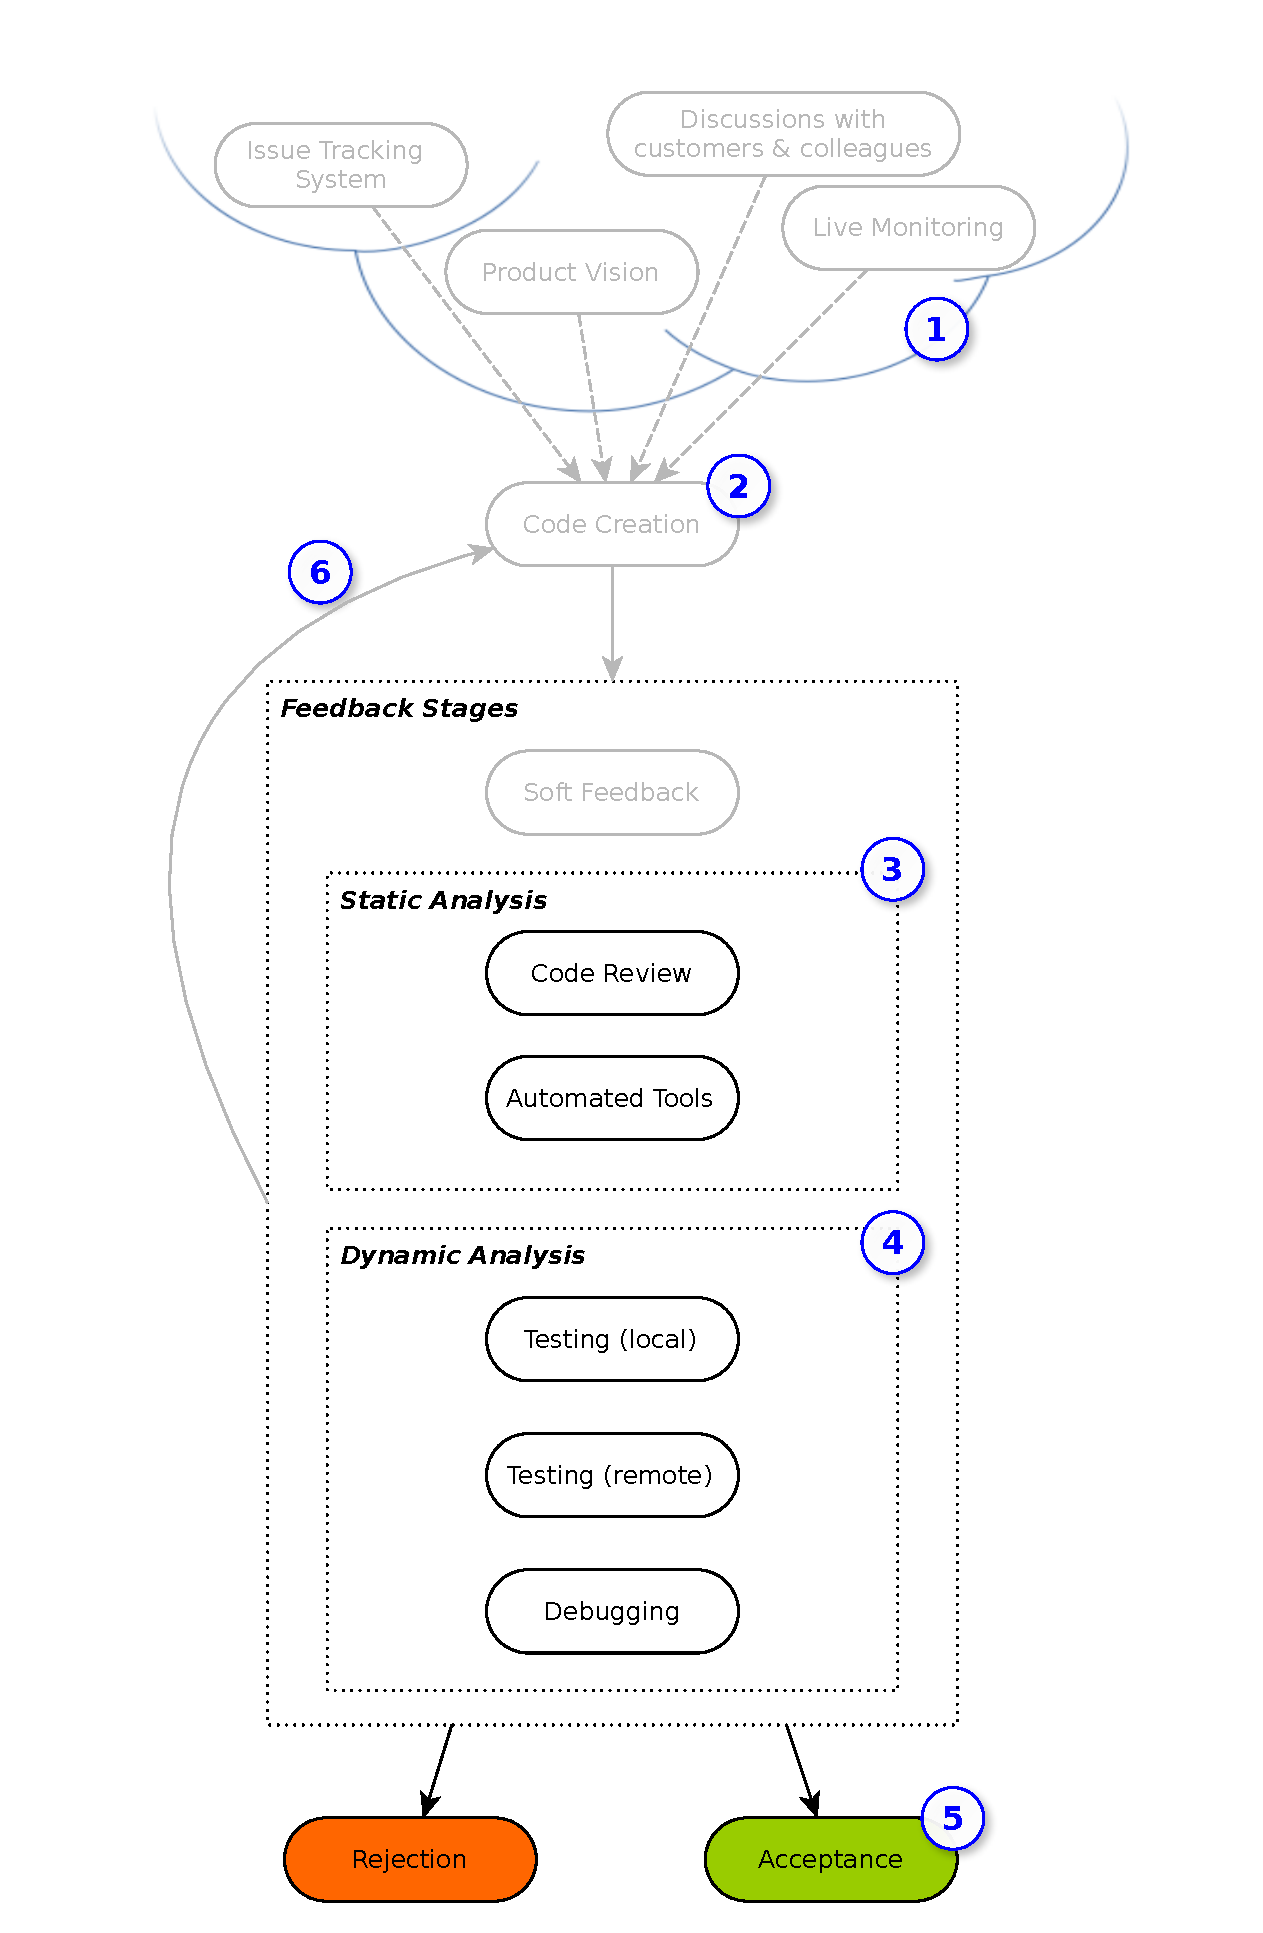
\includegraphics[width=0.65\columnwidth]{development_model_without_papers}
% 	\caption{The stages of the FDD model and their relationship to other
%           Software Engineering concepts.}
% 	\label{fig:devmodel}
% \end{figure}

We also have lists:

\begin{enumerate}
  \item Static Analysis~\circled{3} examines program artifacts or
    their source code without executing them~\cite{wichmann1995industrial}, while
 \item Dynamic Analysis~\circled{4} relies on information gathered from their
   execution~\cite{cornelissen2009systematic}.
\end{enumerate}

Or boxes:

\begin{framed}
This thesis is concerned with the empirical assessment of the state of the art of how developers
drive software development with the help of feedback loops. \cite{boyer2020dynamics}
\end{framed}

Or code:
\begin{lstlisting}[caption={\textsc{TrinityCore}},label={lst:e1}]
 x += other.x;
 y += other.y;
 z += other.y;
\end{lstlisting}


I hope this helps you get started!
Moritz

First time should be long: \gls{GCD}
Next time should be short: \gls{GCD}

% \chapter{Sensing Soft Robots' Shape with Cameras: An Investigation on Kinematics-Aware SLAM}
\chapter{Shape Sensing with Cameras: An Investigation on Kinematics-Aware SLAM}
\label{chp:srslam}

\begin{foreword}
    Before we can develop advanced soft robot controllers, we require access to state information. Specifically, we need to know the configuration of the soft robot, which, as introduced in Chapter~\ref{chp:background}, is for soft robots usually defined as the parametrized shape of the backbone.
    In this chapter, we demonstrate how we can augment in a plug-and-play fashion existing state-of-the-art \gls{SLAM} algorithms with kinematic knowledge to achieve shape sensing for soft robots.
\end{foreword}

\begin{abstract}
    % The nature of continuum soft robots calls for novel perception solutions, which can provide information on the robot's shape while not substantially modifying their bodies' softness. One way to achieve this goal is to develop innovative and completely deformable sensors. 
    One way to achieve proprioception of the soft robot's shape while not substantially modifying their bodies' softness is to develop innovative and completely deformable sensors. 
    However, these solutions tend to be less reliable than classic sensors for rigid robots. As an alternative, we consider here the use of monocular cameras. By admitting a small rigid component in our design, we can leverage well-established solutions from mobile robotics. We propose a shape-sensing strategy that combines a SLAM algorithm with nonlinear optimization based on the robot's kinematic model. We prove the method's effectiveness in simulation and with experiments of a single-segment continuous soft robot with a camera mounted to the tip. We achieve mean relative translational errors below 9\% simulations and experiments alike and as low as 0.5\% on average for some simulation conditions.
\end{abstract}

\blfootnote{
    This chapter is partly based on \faFileTextO~\emph{E. Rosi*, \textbf{M. Stölzle}*, F. Solari, and C. Della Santina (2022, April). Sensing Soft Robots' Shape with Cameras: an Investigation on Kinematics-Aware SLAM. In 2022 IEEE 5th International Conference on Soft Robotics (RoboSoft) (pp. 795-801). IEEE.}~\citep{rosi2022sensing}.

    % \nth{1}-author contributions: E. Rosi implemented the methodology, collected the simulation results, and executed the lab experiments with a soft segment. M. Stölzle provided guidance on the methodology, helped debug the implementation of the approach in code, contributed to the experimental setup (e.g., motion capture system, fabrication of the soft segment), and wrote the paper.

    C.D.S. conceived and led the project.
    E.R. implemented the methodology, collected the simulation results, and executed the lab experiments with a soft segment.
    M.S. contributed ideas to the methodology, helped debug the implementation of the approach in code, contributed to the experimental setup (e.g., motion capture system, fabrication of the soft segment), and wrote the paper.
    C.D.S., E.R., and M.S. revised the manuscript.
    C.D.S, F.S., and M.S. supervised the research project.
    C.D.S. provided funding.
}


%% Start the actual chapter on a new page.
\newpage

\section{Introduction}\label{sec:srslam:introduction}
%
With their bodies entirely made of soft deformable materials, continuum soft robots are especially suited for application domains involving safe and robust interaction with humans and environment, and ranging from inspection, to healthcare and agriculture~\cite{majidi2014soft,elfferich2021soft}. To achieve these goals, soft robots must first master the art of controlling and sensing their body shape in space \cite{della2023model}.
%
% We refer to the estimation of the robot shape uniquely from on-board sensors as propriocetive shape sensing.
%
% Methods widely used in rigid robotics are not always applicable to soft systems, and what can be achieved in a simple way for rigid bodies may not be such for soft ones. One relevant example is the 
% ... challenge of sensing the robot's configuration, which in rigid robots can be achieved with well established technologies as encoders placed at the joint. 
%
A major challenge with shape perception in soft robots is that sensing strategies must not compromise the intrinsic softness of these systems~\cite{polygerinos2017soft,wang2018toward}. %In the literature they mainly propose resistive, capacitive and magnetic sensors to achieve proprioception \cite{cianchetti2012sensorization,polygerinos2017soft,atalay2017batch,atalay2018highly}.
%
% One way to achieve this goal is to look for . 
To this end, researchers have proposed several entirely deformable sensors over the years, including capacitive~\cite{scimeca2019model},  and optical sensors~\cite{li2021scaling}, liquid metal~\cite{wall2017method}. These solutions are quite attractive since they minimally corrupt the physical softness of the robot. However, they usually require complex learning strategies to be used since their behavior is hard to model~\cite{thuruthel2019soft,truby2020distributed}.
%
% wall an brock sousace finger
% moritz otpmized sensing

An alternative is to relax the constraint of complete deformability and allow from small rigid components. This strategy enables rethinking the use of existing sensing technologies in this radically new context. Examples are hall sensors~\cite{guo2019continuum}, IMUs~\cite{hughes2020sensing}, and microphones~\cite{zoller2018acoustic}. %wall and brock
%
The information gathered from inward-facing cameras looking at features in soft chambers' inner walls has proven sufficient to estimate the configuration~\cite{she2020exoskeleton,werner2020vision}, and characterize contacts with the environment \cite{ward2018tactip,lin2020curvature}. However, all these strategies need machine learning to transform the image information in the desired physical quantity.
%
%Classical image filters for feature extraction are combined with \gls{SVR} to estimate a tip position from the camera images. % Their approach performs similarly to a performance baseline made with an off-the-shelf distance sensor used to measure the linear extension.
%
% Another research by Wongwilai et al.~\cite{wongwilai2014slam} proposes a framework that combines all grasping tasks (object model acquisition, grasping point calculation and navigation of the robotic arm) with a RGB-D \gls{SLAM}.
%
% In contrast, fewer papers explore the use of camera images for proprioception. Weber et al.~\cite{weber2012multi} use an array of micro-cameras which face the environment to estimate the configuration of a single segment robot. The algorithm employs a configuration estimation refinement followed by a full \gls{BA}. 
%
%Cheng et al.~\cite{cheng2020approximate} present a kinematic equivalent model for a planar continuum robot. They build an Approximate \gls{PCC} model, using classical rigid linkages (2L-5R). They also propose a configuration estimation of the planar continuum robot using a monocular camera as an application to their model.
%
%\textbf{\cite{wang2018robot}} they combine SLAM and manipulation for a humanoid robot (Atlas).
%
%\textbf{\cite{klingensmith2016articulated}} they use RGB-D SLAM for estimating joint angles of an articulated manipulator. 
%
%\textbf{\cite{wongwilai2014slam}} they use SLAM for grasping (depth camera). they combine the process of data acquisition, navigation and grasp point calculation together.
%
Alternatively, cameras mounted outwards on the robot's tip and have been used to execute visual servoing~\cite{homberg2019robust}.
% more citations: wang2013visual
%
In the best of Authors' knowledge, the only two works dealing with continuum (non-soft) robots are \cite{weber2012multi} and \cite{cheng2020approximate}.
% 
The first uses \gls{BA} to integrate the output of multiple cameras embedded in a single segment. The second uses hand-tuned features to estimate the robot configuration within a novel kinematic model. Thus, no general strategy to estimate the whole state of a soft segment from a single monocular camera exists in the literature.

\gls{SLAM} is one of the most effective and largely used strategies for vision-based localization for mobile robots and autonomous vehicles~\cite{fuentes2015visual,mur2017orb}. %SLAM has been used been widely used in autonomous vehicles \cite{x} and rigid robots~\cite{klingensmith2016articulated}.
%
In this work, we investigate using monocular \gls{SLAM} to estimate the location of selected points across the soft robot. We then propose a mechanism for simultaneously refining the estimation and reconstructing the complete shape of the robot. We do that by retracting the output of the \gls{SLAM} to the manifold of camera configurations admitted by the kinematic model of the soft robot. We formulate this action as a nonlinear optimization problem. Fig.~\ref{fig:srslam:method_overview} summarizes the proposed architecture. We test the strategy with simulations and experiments, achieving mean relative translational errors between \SI{0.4}{\percent} and \SI{9}{\percent} in the former, and from \SI{5}{\percent} to \SI{9}{\percent} in the latter.

\begin{figure*}[ht]
     \centering
     \subfigure[Overview]{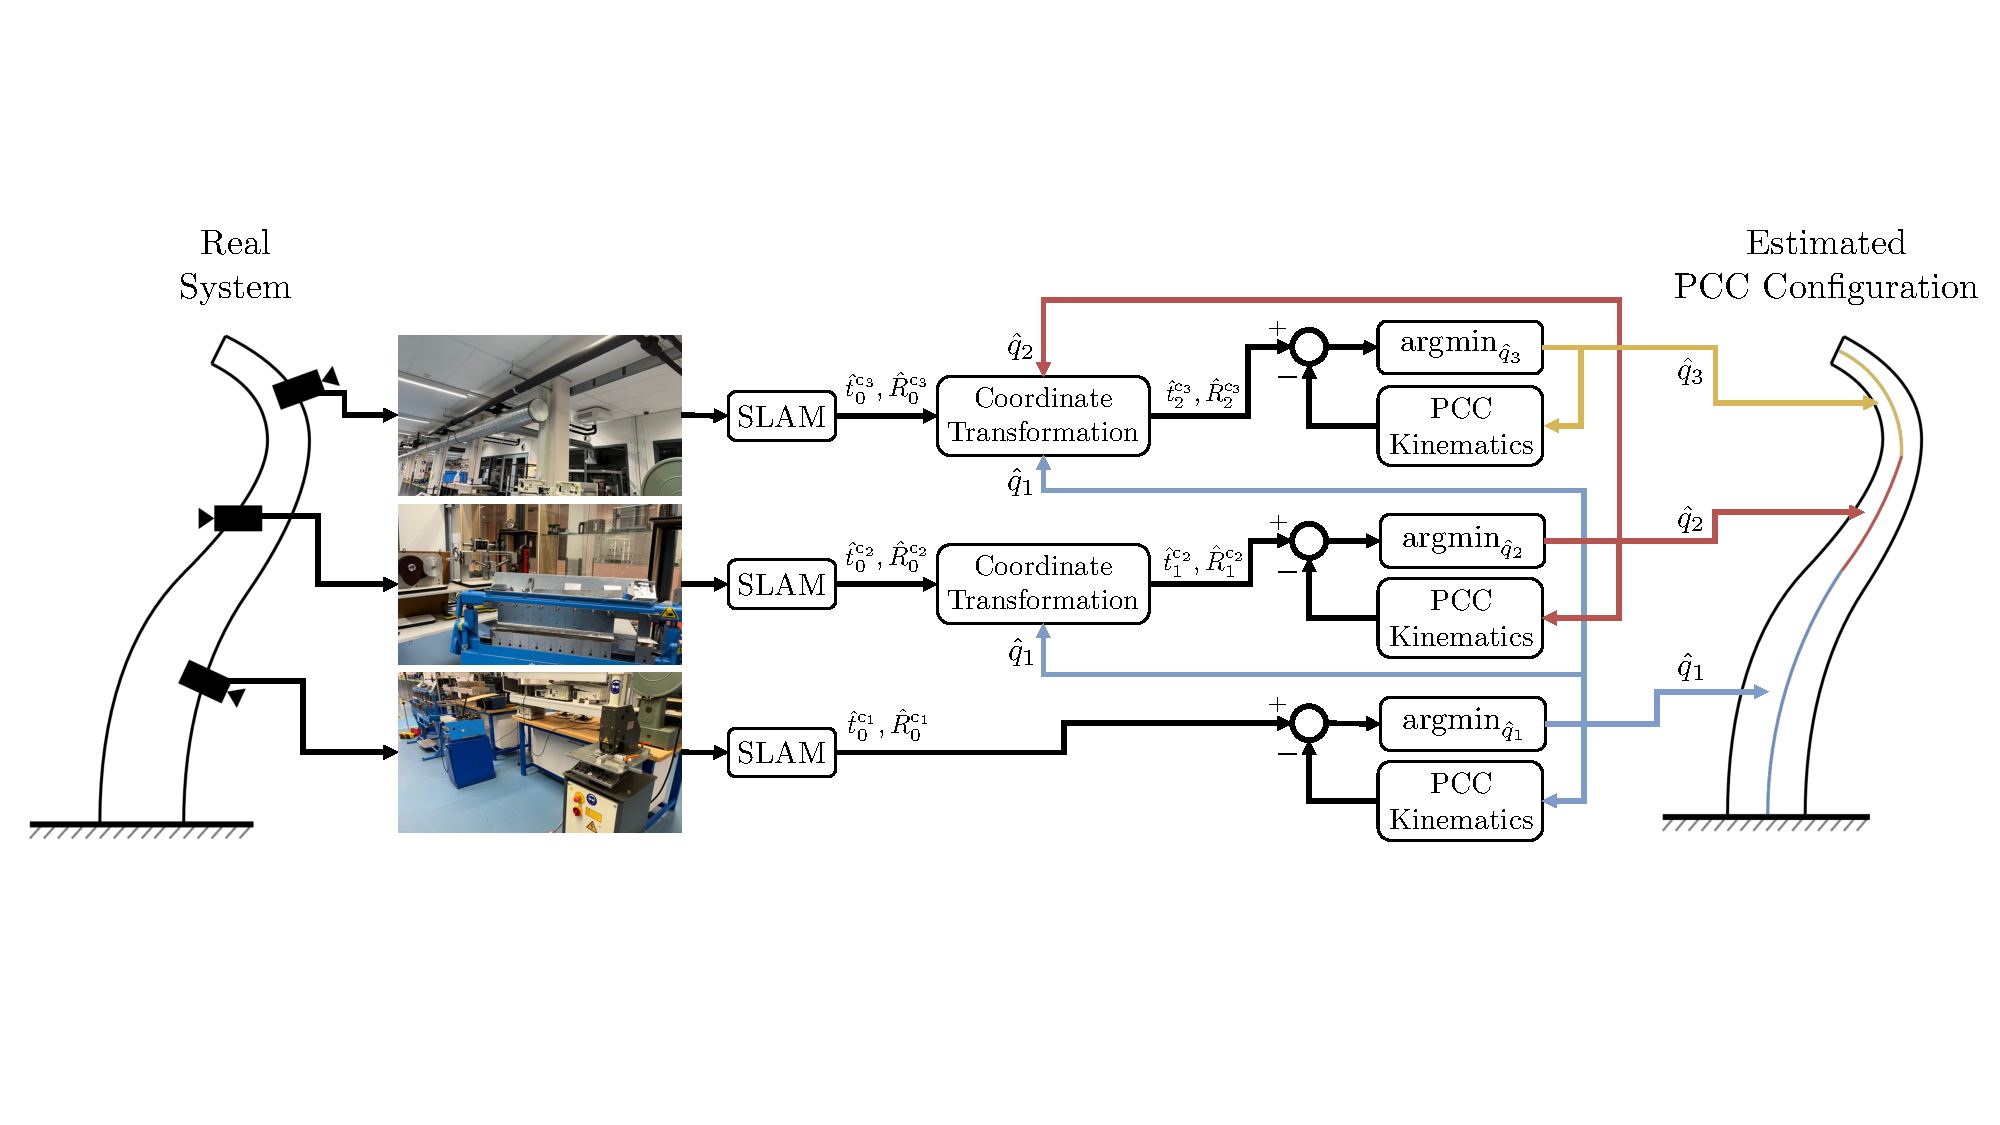
\includegraphics[width=0.69\columnwidth]{srslam/figures/graphic_method_overview_v5_cropped.pdf} \label{fig:srslam:method_overview}}
     \subfigure[Kinematics]{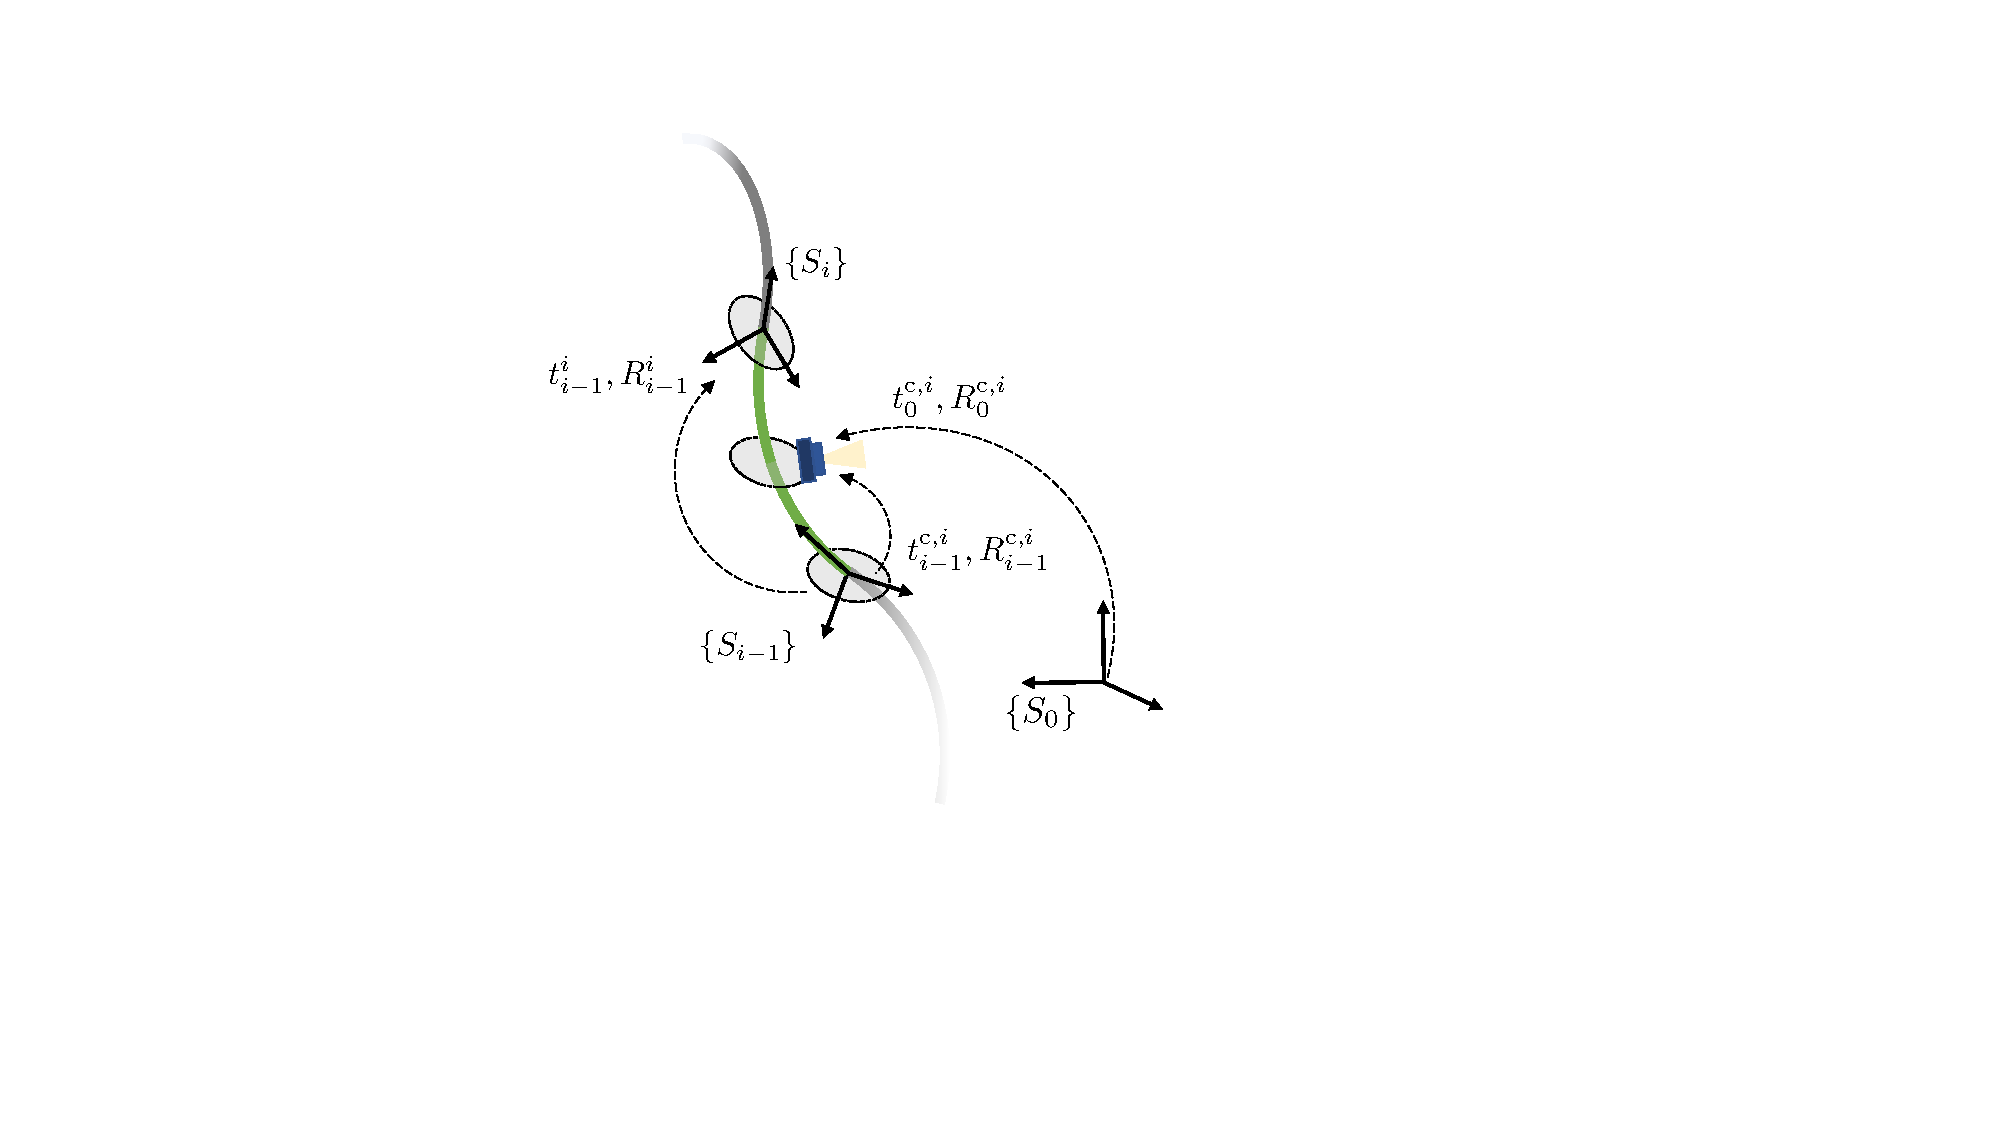
\includegraphics[width=0.24\columnwidth, trim = {0 0 0 0}, clip]{srslam/figures/kinematics_v2.pdf}\label{fig:srslam:kinematic_parameters} \label{fig:srslam:kinematics}}
     \caption{ Panel (a) shows a pictorial representation of the proposed perception strategy. Cameras are attached to a soft continuum robot. We propose to use ORB-SLAM~\cite{mur2017orb} to gather a pose estimate for each camera. The results are iteratively combined to extract local transformation, and refined by projecting the resulting postures onto the manifold of configurations attainable with the \gls{PCC} kinematics. The result is an estimation of the full shape within the selected kinematic description $\hat{q}$. Panel (b) reports the main quantities of the kinematic model of one segment. }
\end{figure*}
\section{Proposed architecture: Shape estimation with kinematics-aware SLAM}
\label{sec:srslam:pose_estimation}

In this work we propose to use \gls{SLAM} for proprioception of continuum soft robots. Common kinematic parametrizations for soft robots such as \gls{PCC}~\cite{webster2010design} or \gls{PCS}~\cite{renda2018discrete} model the soft arm to consist of multiple segments with independent kinematic state variables. 
In the following, we assume that the robot's model consists of $n_{\mathrm{S}}$ segments, and that a monocular camera is attached to each segment. We rely on a \gls{PCC} kinematic formulation. However, the proposed results can be directly generalized to the PCS case.
%
%We expect that there exists a constant coordinate transformation between the camera and one point along the center-line of the soft segment.
%
Our goal is to reconstruct the full shape (i.e., a configuration $q_i$ for each segment) of the soft robot from the stream of images recorded by the cameras.

Fig. \ref{fig:srslam:method_overview} shows an overview of the proposed architecture.
%
%Monocular \gls{SLAM} algorithms are able to estimate the pose of each camera as the robot arm follows a trajectory.
We use \gls{SLAM} algorithms such as monocular ORB-SLAM~\cite{mur2017orb} to estimate the pose of cameras attached to the soft robotic arm.  The pose estimation consists of 3D translation and rotations describing the relative camera movement from initial calibration to the current state ($\hat{t}_0^{\mathrm{c}_i},\hat{R}_0^{\mathrm{c}_i}$ in the figure). Then, the kinematic model is simultaneously used to refine the outputs of the SLAM and transform it to the desired estimation of the configurations ($\hat{q}_1,\hat{q}_3,\hat{q}_3$ in the figure). Starting from the base segment, and progressively iterating up until reaching the tip of the robot, we express translation and rotations in local coordinates, and we optimize the estimated configurations segment-by-segment starting at the proximal end by projecting the pose estimate into the 3D \gls{PCC} kinematics.
% This approach leverages known characteristics of the continuum soft robot and reduces the pose estimation error.

In the following subsections, we provide more details on the various components of this architecture.

\subsection{Background: Monocular ORB-SLAM}
We choose monocular ORB-SLAM~\cite{mur2017orb} for pose estimation of the camera locations. Although this technological solution has never been applied to soft robots, the algorithm itself is well established and its applications to mobile robotics widespread. As such, we  briefly describe here only the major steps of the algorithm.%, based on the pipeline in \ref{fig:srslam:algorithmpipeline}. 
 \begin{enumerate}
     \item \textbf{Map Initialization}: ORB-SLAM initializes a map of 3D points based on two video frames. The 3D points and relative camera pose are computed using triangulation of 2D ORB feature correspondences.
     \item \textbf{Tracking}: Once the map is initialized, the camera pose is estimated for each new frame by matching features in the current frame to features in the last key frame. The estimated camera pose is refined by tracking the local map.
     \item \textbf{Local Mapping}: If the current frame is identified as a key frame, it is used to create new 3D map points. At this stage, \gls{BA} is used to minimize re-projection errors by adjusting the camera pose and 3D points.
     \item \textbf{Loop Closure}: Loops are detected for each key frame by comparing it against all previous ones. % key frames using the bag-of-features approach~\cite{o2011introduction}. 
     %Any time a loop closure is detected, the pose graph is optimized to refine the camera poses of all the key frames.
     This information is used to optimize the poses.
 \end{enumerate}
An important aspect of \gls{SLAM} algorithms are key frames, which are a subset of video frames that contain cues for localization and tracking. Two consecutive key frames usually involve sufficient visual change. % In the end the algorithm returns the camera poses for each key frame.

\subsection{Projection into PCC-Kinematics}
Once the \gls{SLAM} algorithm provides us with the estimated camera poses, we want to interpret and correct them such as that they are coherent with the \gls{PCC} kinematic model.
%
In this paper, we consider the \emph{Delta} parametrization~\cite{della2020improved} of the \gls{PCC} kinematics, but the formulation could also be easily adapted to other kinematic parametrizations such as \gls{PCS}~\cite{renda2018discrete}.

% \begin{figure}[ht]
%     \centering
%     \includegraphics[width=1\columnwidth]{srslam/figures/kinematic_parameters.pdf}\label{fig:srslam:kinematic_parameters}
%     \\
%     \caption{One graphic showing the kinematic parameters for a multi-segment setup with multiple cameras and all used coordinate transformations.}
% \end{figure}

We show a pictorial representation of this kinematic model in Fig. \ref{fig:srslam:kinematics}. Each segment of original length $L_{0,i}$ is described with three configuration variables 
%
%\begin{equation}
    $q_i \in \mathbb{R}^{3} = \begin{pmatrix}\Delta_{x,i} & \Delta_{y,i} & \delta L_i\end{pmatrix}^\mathrm{T}$,
%\end{equation}
where $\delta L_i$ is segment's extension, and $\Delta_{x,i}$ and $\Delta_{y,i}$ are the differences of the arc lengths of the segment at a radial distance of $d_i$ from the center-line along both cardinal directions of the base~\cite{della2020improved}. The complete robot's configuration is $q \in \mathbb{R}^{3 n_{\mathrm{S}}}$. The coordinate transformation for segment $i$ from the base frame $\{ S_{i-1} \}$ into the tip frame $\{ S_{i} \}$ as a function of the configuration $q_i$ is given by~\cite{della2020improved}
\begin{equation}
\label{eq:srslam:transformation_improved_pcc}
\begin{split}
    R_{i-1}^{i} &= 
    \begin{pmatrix}
        1 + \frac{\Delta_{x,i}^2}{\Delta_{i}^2} \left ( \mathrm{c}_i - 1 \right ) & \frac{\Delta_{x,i} \Delta_{y,i}}{\Delta_{i}^2} \left ( \mathrm{c}_i - 1 \right ) & \frac{\Delta_{x,i}}{\Delta_i} \mathrm{s}_i\\
        \frac{\Delta_{x,i} \Delta_{y,i}}{\Delta_{i}^2} \left ( \mathrm{c}_i - 1 \right ) & 1 + \frac{\Delta_{y,i}^2}{\Delta_{i}^2} \left ( \mathrm{c}_i - 1 \right ) & \frac{\Delta_{y,i}}{\Delta_i} \mathrm{s}_i\\
        \frac{-\Delta_{x,i}}{\Delta_i} \mathrm{s}_i & \frac{-\Delta_{y,i}}{\Delta_i} \mathrm{s}_i & \mathrm{c}_i
    \end{pmatrix},\\
    \vspace{0.25em}
    t_{i-1}^{i} &= \frac{d_i ( L_{0,i}+\delta L_i)}{\Delta_i^2}
    \begin{pmatrix}
        \Delta_{x,i} (1 - \mathrm{c}_i) & \Delta_{y,i} (1 - \mathrm{c}_i) & \Delta_{i} \mathrm{s}_i
    \end{pmatrix}^{\mathrm{T}},
\end{split}
\end{equation}
where we substituted $\Delta_i = \sqrt{\Delta_{x,i}^2 + \Delta_{y,i}^2}$, $\mathrm{s}_i = \sin \left ( \frac{\Delta_i}{d_i} \right )$, and $\mathrm{c}_i = \cos \left ( \frac{\Delta_i}{d_i} \right )$ for conciseness.

We describe the coordinate frame of camera $i$ with $\{ S_{\mathrm{c}_i} \}$. It is assumed that there exists a fixed transformation $T_{\check{\mathrm{c}},i}^{\mathrm{c}_i} \in \mathbb{R}^{4 \times 4}$ from frame $\{ S_{\check{\mathrm{c}},i} \}$ to the camera frame $\{ S_{\mathrm{c}_i} \}$. 
$\{ S_{\check{\mathrm{c}},i} \}$ is localized at a distance $l_{\mathrm{c}_i}$ along the center-line from the base of segment $i$. 
The transformation $T_{i-1}^{\check{\mathrm{c}},i}(q_{\check{c},i})$ from the base to the frame $\{ S_{\check{\mathrm{c}},i} \}$ can be found with \eqref{eq:srslam:transformation_improved_pcc} by plugging in the adjusted configuration $q_{\check{c},i}$ defined as
\begin{equation}\label{eq:srslam:camera_configuration}
    q_{\check{c},i} = \frac{l_{\mathrm{c}_i}}{L_{0,i}} q_i,
\end{equation}
and the adjusted original length  $l_{\mathrm{c}_i}$.

The \gls{SLAM} algorithm provides a pose estimate for the translation $\hat{t}_{\mathrm{c},\mathrm{t}0,i}^{\mathrm{c}_i} \in \mathbb{R}^3$ and rotation $\hat{R}_{\mathrm{c},\mathrm{t}0,i}^{\mathrm{c}_i} \in \mathbb{R}^{3 \times 3}$ relative to the known initial reference frame of the camera $\{ S_{\mathrm{c},\mathrm{t}0,i} \}$. 
Thus, we first transform the pose estimates to the inertial frame of the robot $\{ S_0 \}$
\begin{equation}
    \begin{pmatrix}
        \hat{t}_{0}^{\mathrm{c}_i}\\
        1
    \end{pmatrix}
    = T_0^{\mathrm{c},\mathrm{t}0,i}
    \begin{pmatrix}
        \hat{t}_{\mathrm{c},\mathrm{t}0,i}^{\mathrm{c}_i}\\
        1
    \end{pmatrix},
    \quad
    \hat{R}_{0}^{\mathrm{c}_i} = R_0^{\mathrm{c},\mathrm{t}0,i} \hat{R}_{\mathrm{c},\mathrm{t}0,i}^{\mathrm{c}_i}.
\end{equation}

We introduce the following notations for the \gls{PCC} kinematics
\begin{equation}\label{eq:srslam:Pi}
\begin{split}
    \hat{t}_{i-1}^{\mathrm{c}_i} &= \Pi_\mathrm{t}(\hat{q}_i) = 
    \hat{T}_{i-1}^{\check{\mathrm{c}},i} \left (\frac{l_{\mathrm{c}_i}}{L_{0,i}} \hat{q}_i \right )
    t_{\check{\mathrm{c}},i}^{\mathrm{c}_i}\\
    \hat{R}_{i-1}^{\mathrm{c}_i} &= \Pi_\mathrm{R}(\hat{q}_i) =
    \hat{R}_{i-1}^{\check{\mathrm{c}},i} \left (\frac{l_{\mathrm{c}_i}}{L_{0,i}} \hat{q}_i \right )
    R_{\check{\mathrm{c}},i}^{\mathrm{c}_i},
\end{split}
\end{equation}
where $\hat{t}_{i-1}^{\check{\mathrm{c}},i}$ and $\hat{R}_{i-1}^{\check{\mathrm{c}},i}$ describe the translation and rotation from the base of the segment to the camera frame according to the \gls{PCC} kinematic model for an estimated configuration of the the segment $\hat{q}_i$. $\hat{T}_{i-1}^{\check{\mathrm{c}},i}(q_{\check{c},i})$ and $\hat{R}_{i-1}^{\check{\mathrm{c}},i}(q_{\check{c},i})$ are based on \eqref{eq:srslam:transformation_improved_pcc} and a function of the adjusted configuration $q_{\check{c},i}$ referenced in \eqref{eq:srslam:camera_configuration}.

Additionally, the pose estimates by the \gls{SLAM} algorithm need to be transformed to the base frame of segment $i$. Thus, we introduce the following
\begin{equation}\label{eq:srslam:Psi}
\begin{split}
    \hat{t}_{i-1}^{\mathrm{c}_i} &= \Psi_\mathrm{t}(q_1 \dots q_{i-1}, \hat{t}_{0}^{\mathrm{c}_i}) =
    \prod_{\tilde{i}=1}^{i-1} \left ( T_{\tilde{i}-1}^{\tilde{i}} \left (\hat{q}_{\tilde{i}} \right )  \right )^\mathrm{T}
    \begin{pmatrix}
        \hat{t}_{0}^{\mathrm{c}_i}\\
        1
    \end{pmatrix},\\
    \hat{R}_{i-1}^{\mathrm{c}_i} &= \Psi_\mathrm{R}(q_1 \dots q_{i-1}, \hat{R}_{0}^{\mathrm{c}_i}) =
    \prod_{\tilde{i}=1}^{i-1} \left ( R_{\tilde{i}-1}^{\tilde{i}} \left (\hat{q}_{\tilde{i}} \right )  \right )^\mathrm{T}
    \hat{R}_{0}^{\mathrm{c}_i}.
\end{split}    
\end{equation}

Next, we define a cost function to optimize the pose estimate by projecting them into the \gls{PCC}-kinematics
% Please note, that we do not include the orientation estimate $\hat{R}_{0}^{\mathrm{c}_i}$ by the \gls{SLAM} algorithm in the cost function.
%
\begin{equation}\label{eq:srslam:cost_fun}
    \min_{\hat{q}} \sum_{i=1}^{n_\mathrm{S}} f_{\mathrm{t},i}(\hat{q}) + \lambda_\mathrm{R} f_{\mathrm{R},i}(\hat{q}),
\end{equation}
with
\begin{equation}\label{eq:srslam:cost_fun_ingredients}
\begin{split}
    f_{\mathrm{t},i}(\hat{q}) &=
    \big\lVert 
    \Pi_\mathrm{t}(\hat{q}_i) - \Psi_\mathrm{t}(q_1 \dots q_{i-1}, \hat{t}_{0}^{\mathrm{c}_i})
    \big\rVert_2,\\
    f_{\mathrm{R},i}(\hat{q}) &=
    \big\lVert 
    \Pi_\mathrm{R}(\hat{q}_i) - \Psi_\mathrm{R}(q_1 \dots q_{i-1}, \hat{R}_{0}^{\mathrm{c}_i})
    \big\rVert_F,
\end{split}
\end{equation}
where the Euclidean norm is used to compute the translational error between the predicted translation by the \gls{PCC} kinematic model and the estimated translation by \gls{SLAM}. The rotational error is weighted with $\lambda_\mathrm{R}$ and computed with the Frobenius norm between the predicted rotation matrix by the \gls{PCC} kinematics and the estimated orientation by \gls{SLAM} represented as a rotation matrix as well.

Please note, that the optimization of the configuration estimate $\hat{q}$ can be decoupled for each segment. 
We start by optimizing the configuration of the first segment $\hat{q}_1$ based on $\Psi_\mathrm{t}(\hat{t}_{0}^{\mathrm{c},1})$ and $\Psi_\mathrm{R}(\hat{R}_{0}^{\mathrm{c},1})$. Next, we optimize the configuration of the second segment $\hat{q}_2$ taking into account the already optimized configuration of segment one in $\Psi_\mathrm{t}(\hat{q}_1, \hat{t}_{0}^{\mathrm{c},2})$ and $\Psi_\mathrm{R}(\hat{q}_1, \hat{R}_{0}^{\mathrm{c},2})$. 
Subsequently, we move on to optimize the remaining segments sequentially as described by Algorithm~\ref{alg:srslampose_estimation}. This procedure is also graphically represented by the right side of Fig. \ref{fig:srslam:method_overview}.

\begin{algorithm}[hbt!]
\caption{Pose estimation for soft robots through SLAM}\label{alg:srslampose_estimation}
\begin{algorithmic}
\REQUIRE $o \in \mathbb{R}^{n_\mathrm{S}}$ \COMMENT{Observations of all cameras}
\ENSURE $\hat{q} \in \mathbb{R}^{3 n_\mathrm{S}}$ \COMMENT{Estimated robot configuration}
\STATE $i \gets 1$
\WHILE{$i \leq n_\mathrm{S}$}
    \vspace{0.25em}
    \STATE $\hat{t}_{0}^{\mathrm{c}_i} \gets T_0^{\mathrm{c},\mathrm{t}0,i} \: \mathrm{SLAM}_\mathrm{t}(o_i)$ \COMMENT{Translational est. SLAM}
    \vspace{0.25em}
    \STATE $\hat{R}_{0}^{\mathrm{c}_i} \gets R_0^{\mathrm{c},\mathrm{t}0,i} \: \mathrm{SLAM}_\mathrm{R}(o_i)$ \COMMENT{Rotational est. SLAM}
    \vspace{0.25em}
    \STATE $f_{\mathrm{t},i}(\hat{q}) \gets
    \big\lVert 
    \Pi_\mathrm{t}(\hat{q}_i) - \Psi_\mathrm{t}(q_1 \dots q_{i-1}, \hat{t}_{0}^{\mathrm{c}_i})
    \big\rVert_2$
    \vspace{0.25em}
    \STATE $f_{\mathrm{R},i}(\hat{q}) \gets
    \big\lVert 
    \Pi_\mathrm{R}(\hat{q}_i) - \Psi_\mathrm{R}(q_1 \dots q_{i-1}, \hat{R}_{0}^{\mathrm{c}_i})
    \big\rVert_F$
    \vspace{0.25em}
    \STATE $f_{c,i}(\hat{q}) \gets f_{\mathrm{t},i}(\hat{q}) + \lambda_\mathrm{R} f_{\mathrm{R},i}(\hat{q})$ \COMMENT{Cost function for $\hat{q}_i$}
    \vspace{0.25em}
    \STATE $\hat{q}_i \gets \argmin_{\hat{q_i}} f_c(\hat{q})$
    \vspace{0.25em}
    \STATE $i \gets i + 1$
\ENDWHILE
\end{algorithmic}
\end{algorithm}

\section{Simulations}
\label{sec:srslam:simulations}

We quantitatively evaluate our approach in simulation for one soft robotic segment with a camera attached to the tip of the robot. 
We first compute trajectories that behave according to \gls{PCC} kinematics. 
Next, we render photo-realistic images for the camera attached to the tip of the segment for every time step using a virtual environment implemented in Blender. Subsequently, we process the synthetic camera images with the ORB-SLAM~\cite{mur2017orb} algorithm and projected the estimated poses of the tip of the segment into the \gls{PCC} kinematic model as outlined in Section~\ref{sec:srslam:pose_estimation}. Finally, we compare the estimated poses against the ground truth and statistically evaluate the \gls{RMSE} both for translational and rotational estimates. More details follow.

\subsection{System}\label{sub:srslam:simulations_system}
We consider a soft robotic segment of diameter \SI{20}{mm} diameter and with varying lengths $L_{0,1}$ between \SI{15}{cm} and \SI{100}{cm}.
As the camera is attached to the tip of the segment, we set $l_{\mathrm{c}_1} = L_{0,1}$ and define $T_{\check{\mathrm{c}},1}^{\mathrm{c},1} = \mathbb{I}^4$.

\subsection{Trajectories and calibration sequence}\label{sub:srslam:trajectories}
Three different trajectories are considered for the simulated movement of the soft robotic segment and its attached virtual camera. While the first one represents a planar side bending, the second one describes an “8” shape with the tip, and the last one covers a lobe of the “8”. 
Those trajectories were commanded in $\Delta_{x,1}$ and $\Delta_{y,1}$, with the following mathematical formulas:
\begin{equation}\label{eq:srslam:trajectory_parametrization}
    \Delta_{x,1} = L_{0,1} A_x \sin(2 \pi f_x) \qquad \Delta_{y,1} = L_{0,1} A_y \sin(2 \pi f_y),
\end{equation}
with $L_{0,1}$ the unextended length of the robot, $A_x$ and $A_y$ amplitudes of the sinusoids and $f_x$ and $f_y$ frequencies of the sinusoids.
The parameters $f_x$ and $f_y$ are defined as follows with $k$ representing the current time index:
\begin{equation}
    f_x = \frac{F_x (k-1)}{n_{\mathrm{t}}}, \qquad f_y = \frac{F_y (k-1)}{n_{\mathrm{t}}}.
\end{equation}
Please note that these trajectories do not contain any segment elongation. 
We list the chosen amplitudes and frequencies of the trajectories in Table~\ref{tab:srslam:trajectory_params}. Each trajectory is generated considering different robot lengths, namely \SI{15}{cm}, \SI{30}{cm} and \SI{100}{cm}. The number of time steps $n_{\mathrm{t}}$ is chosen at $120$. 
The commanding of $\Delta_{x,1}$ and $\Delta_{y,1}$ is such that the amplitude and frequency of the trajectory are independent of the number of frames (i.e., time steps).
In Figure~\ref{fig:srslam:trajectories}, we show a 3D visualization of the trajectories corresponding to a segment length of \SI{15}{cm}.

\begin{table}
\centering
\caption{Parameters of the implemented trajectories. We list the amplitudes and the frequencies of the trajectories parametrized by $\Delta_{x,1}$ and $\Delta_{y,1}$ as specified in \eqref{eq:srslam:trajectory_parametrization}.}
% \begin{scriptsize}
\begin{tabular}{lcccc}\toprule
\textbf{Trajectory} & $A_x$ & $A_y$ & $F_x$ & $F_y$\\
\midrule
Trajectory 1: planar side bending & 0.1 & 0 & 0.5 & 0\\
Trajectory 2: half 8-shape & 0.05 & 0.05 & 1 & 0.5\\
Trajectory 3: full 8-shape & 0.05 & 0.05 & 2 & 1\\
\bottomrule
\end{tabular}
% \end{scriptsize}
\label{tab:srslam:trajectory_params}
\end{table}

\begin{figure*}[ht]
  \centering
  \subfigure[Trajectory 1]{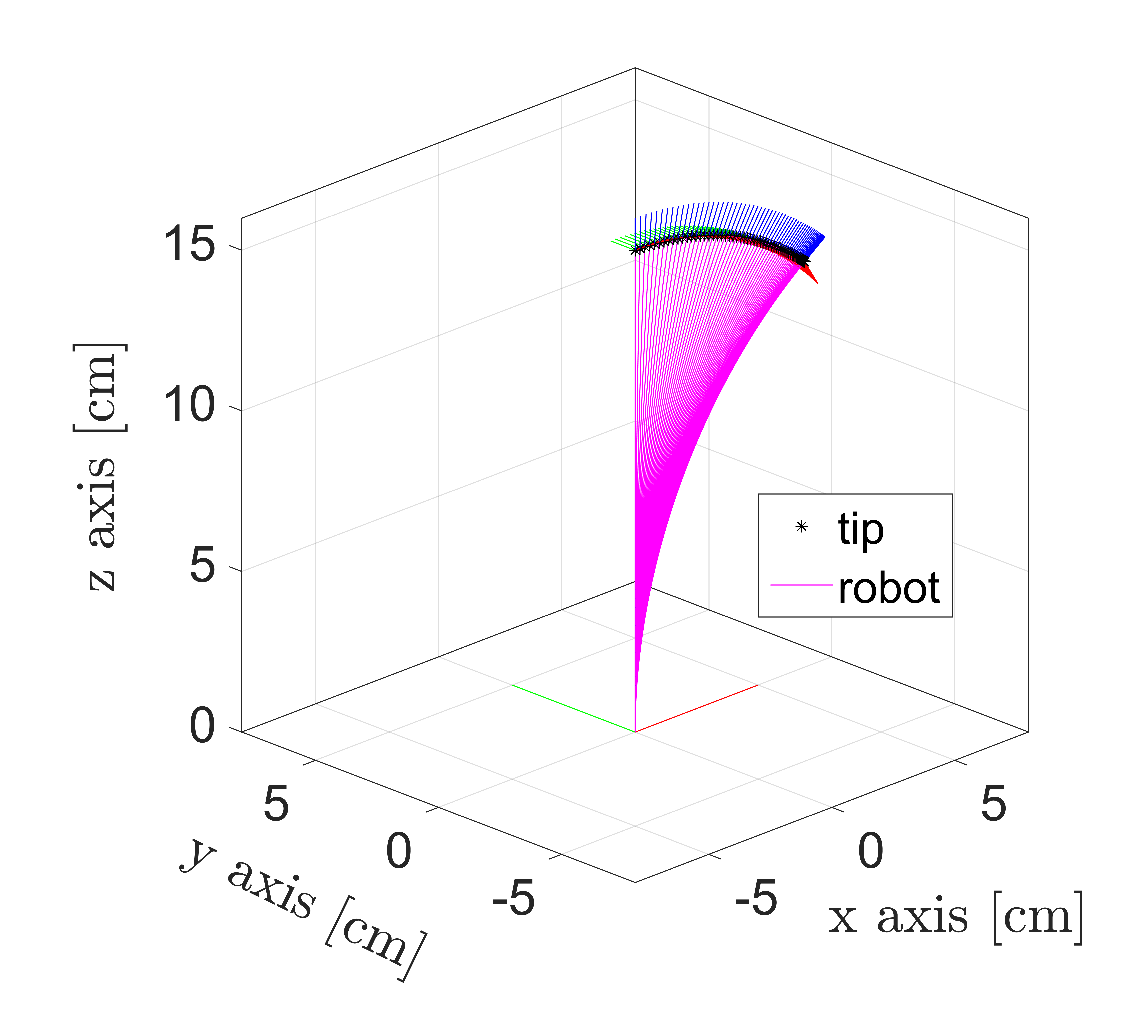
\includegraphics[width=0.21\textwidth]{srslam/figures/t1_l15_v3.0.eps}\label{fig:srslam:traj1}}
  \hspace{0.005\textwidth}% \hfill% or \hspace{5mm} or \hspace{0.3\textwidth}
  \subfigure[Trajectory 2]{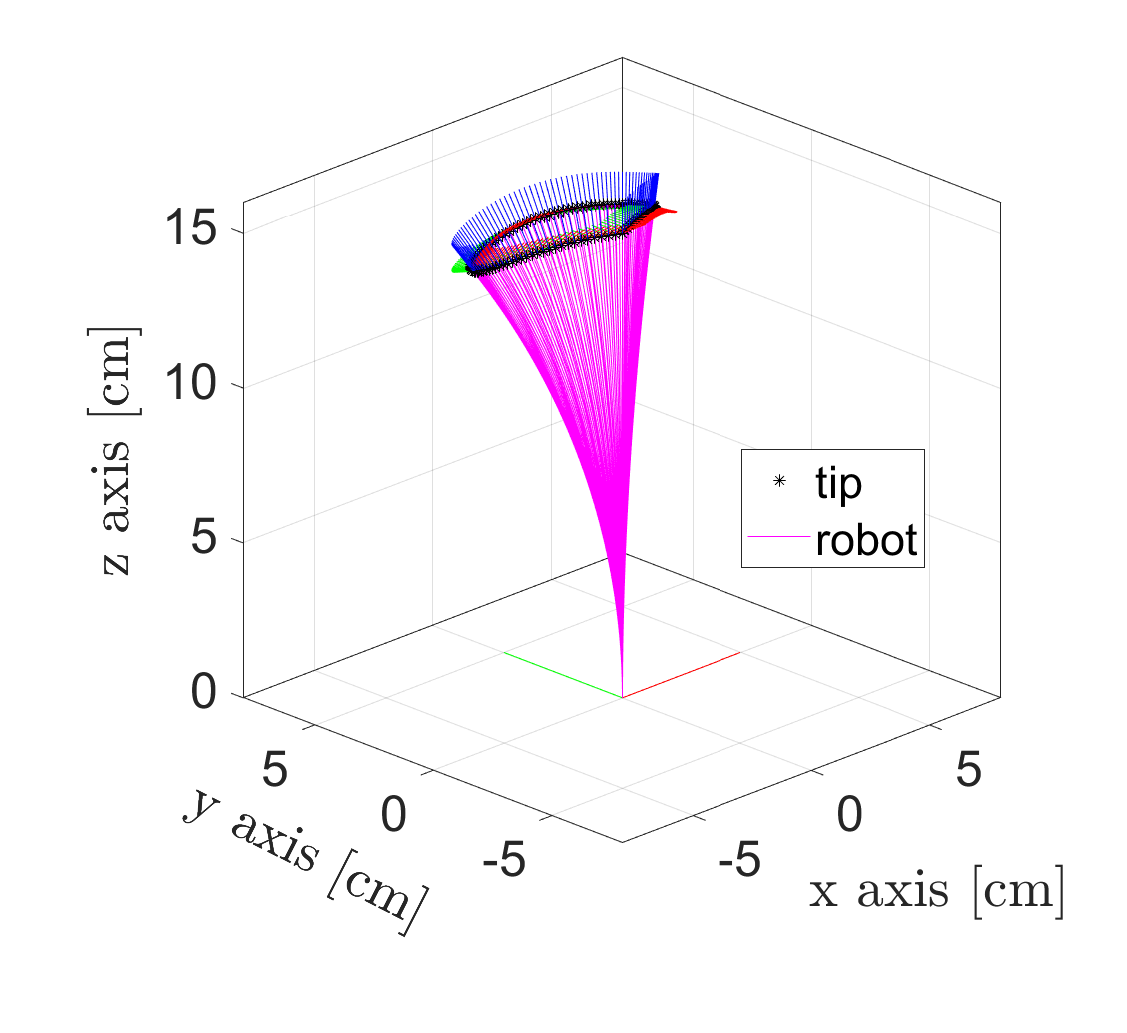
\includegraphics[width=0.21\textwidth]{srslam/figures/t2_l15_v3.2.eps}\label{fig:srslam:traj2}}\hspace{0.005\textwidth}% \hfill% or \hspace{5mm} or \hspace{0.3\textwidth}
  \subfigure[Trajectory 3]{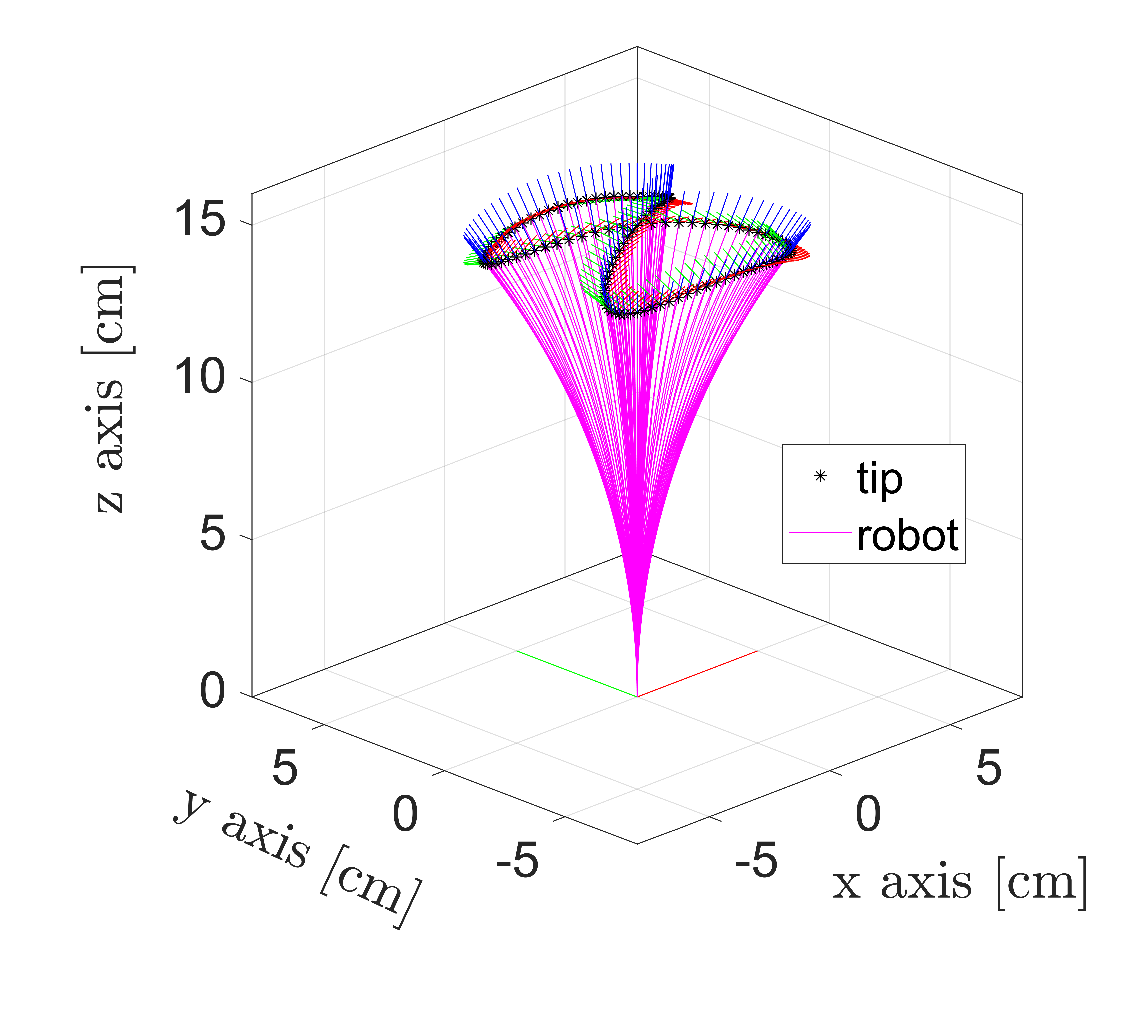
\includegraphics[width=0.21\textwidth]{srslam/figures/t3_l15_v3.1.eps}\label{fig:srslam:traj3}}\hfill
  \subfigure[Virtual interior scene]{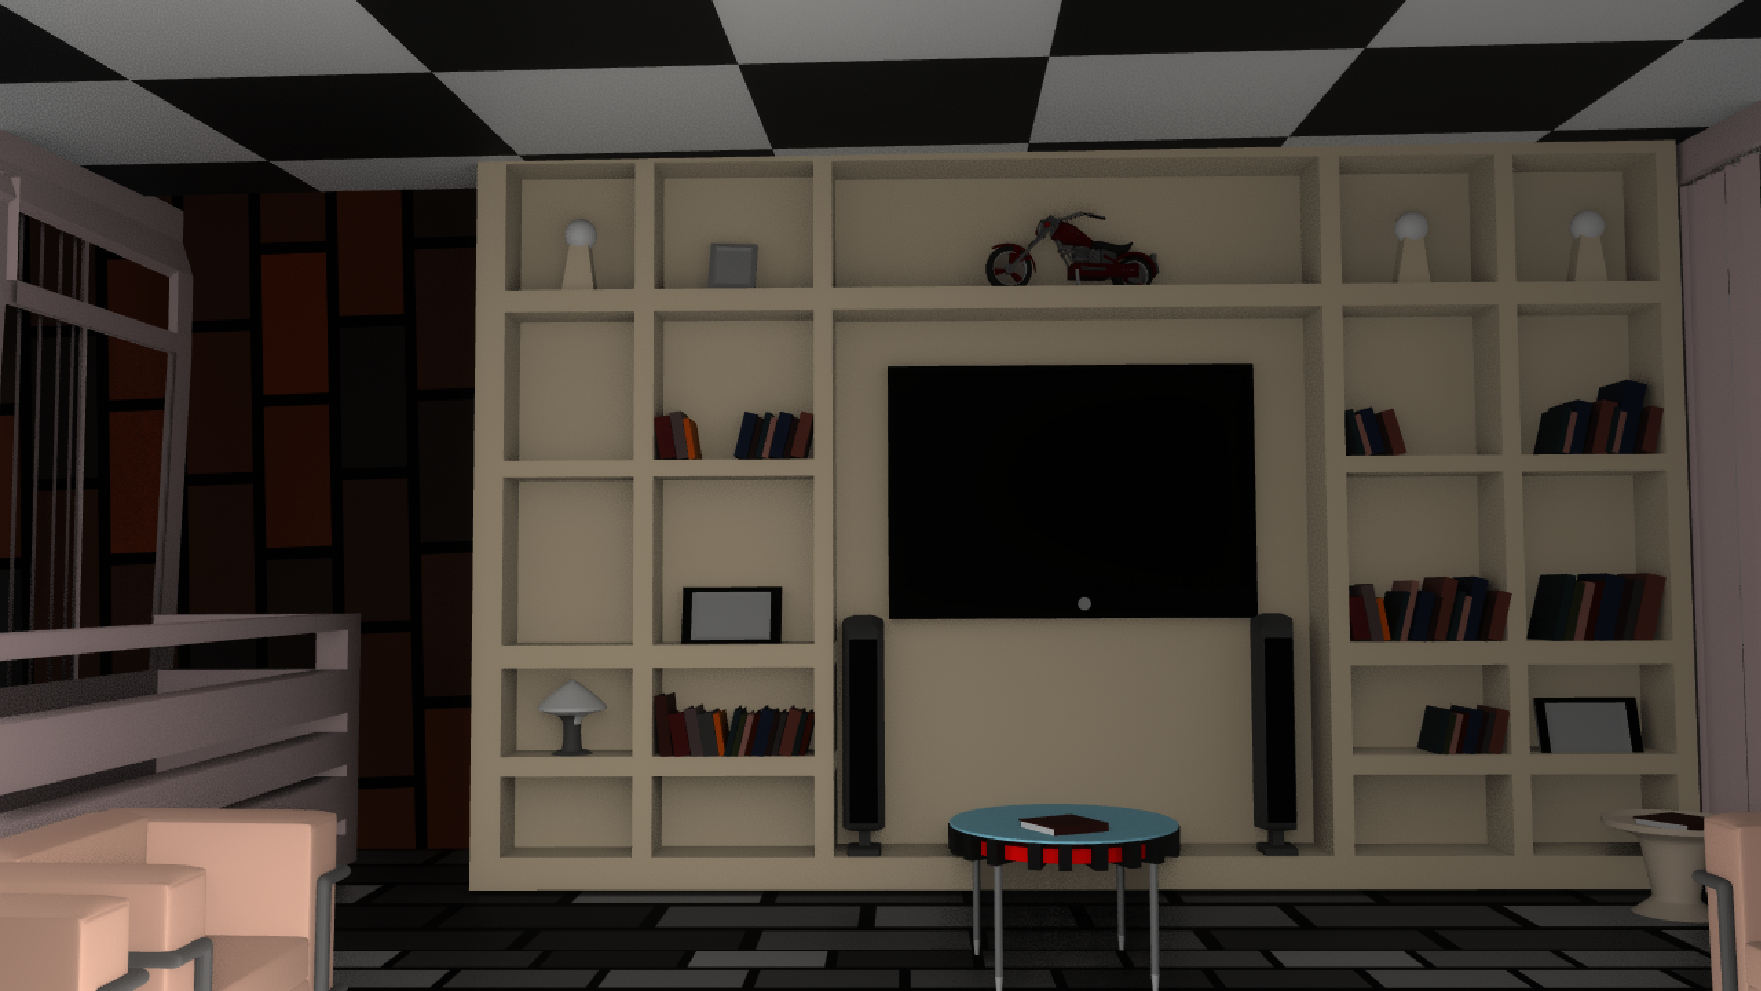
\includegraphics[width=0.3\textwidth]{srslam/figures/interior_scene.pdf}\label{fig:srslam:interior_scene}}
  \caption{3D visualization of the three trajectories used in our simulations and experiments for a segment with \SI{15}{cm} length. In magenta, we visualize the trajectory of the full robot, and in black, the tip positions. Additionally, the tip orientation (red = x-axis, green = y-axis, blue = z-axis) is displayed. The virtual interior scene used for the Blender renderings is presented in the last column.}
  \label{fig:srslam:trajectories}
\end{figure*}

In addition to the robot trajectory, a calibration sequence trajectory is designed to initialize the \gls{SLAM} map. 
It is good practice to move the camera parallel to the scene captured. Accordingly, we decide to move the camera into the $x$ cardinal direction of the segment base frame with the translation distance proportional to the robot length.

\subsection{Rendering of synthetic images}
The rendering software Blender allows us, among other things, to load a 3D model of the environment, follow customized trajectories with a virtual camera, and render photo-realistic synthetic pictures of the environment from the chosen camera perspective. We use an interior scene published by \href{https://www.nextwavemultimedia.com/html/3dblendermodel.html}{Nextwave Multimedia}. We report a view of the scene in Fig. \ref{fig:srslam:interior_scene}.
The virtual camera is set to be perspective with a focal length of \SI{30}{mm}.
For each run, we randomly initialize the trajectory at one of seven predefined launch points in the indoor environment to diversify the coverage of the environment.
The x-, y-, and z-coordinates of the seven initial positions have a standard deviation of \SI{0.5}{m}, \SI{0.2}{m}, \SI{0.4}{m} respectively. The initial orientation represented in XYZ Euler angles varies with a standard deviation of \SI{0.05}{rad}, \SI{0.13}{rad}, and \SI{1.17}{rad}.
For each trajectory, we render $120$ synthetic images along the trajectory and save them to a folder for later offline processing by the ORB-SLAM~\cite{mur2017orb} algorithm. Fig. \ref{fig:srslam:sequences_of_stills_simulations_cropped} reports a few representative stills of what the robot sees during one execution of the three trajectories discussed above.

\begin{figure*}
    \centering
    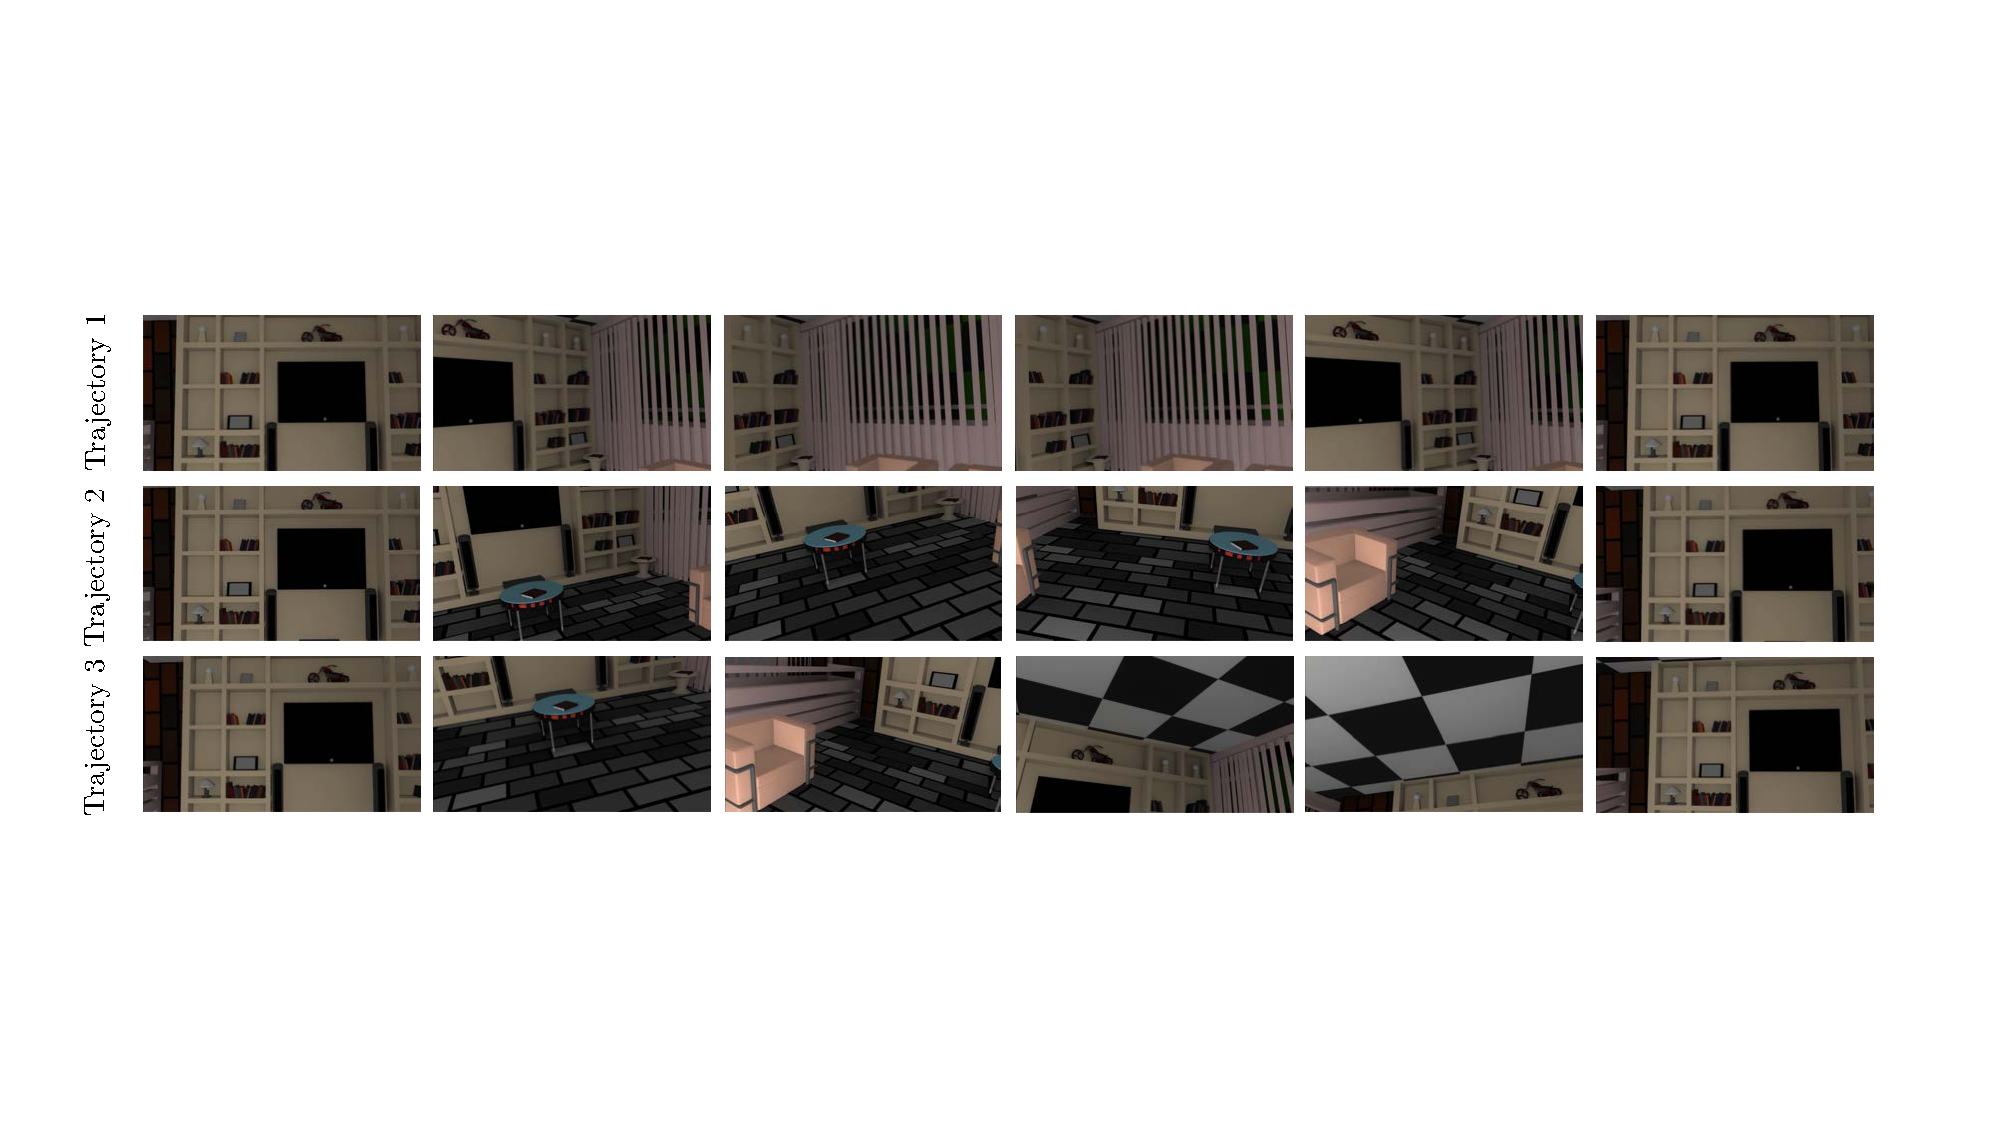
\includegraphics[width=0.9\textwidth]{srslam/figures/graphic_sequences_of_stills_simulations_compressed.pdf}
    \caption{Sequence of stills showing the rendered images by the virtual camera in Blender for three different trajectories and a robot segment of length \SI{15}{cm}. The trajectories are visualized in Figure~\ref{fig:srslam:trajectories}.}
    \label{fig:srslam:sequences_of_stills_simulations_cropped}
\end{figure*}

\subsection{Implementation of ORB-SLAM}
The synthetic images along the trajectory are processed offline by the ORB-SLAM~\cite{mur2017orb} algorithm. We rely on the official MATLAB implementation of ORB-SLAM. While we run our simulations offline to decouple any delays by the rendering and/or \gls{SLAM} pipeline, we would like to point out that other ORB-SLAM implementations, such as, for example, in C++, are able to be run in real-time at frame rates of between \SI{10}{Hz} to \SI{30}{Hz}~\cite{mur2017orb}.

\subsection{Projection into PCC kinematics}
The trade-off parameter $\lambda_\mathrm{R}$ between the rotational and the translational error in the cost function \eqref{eq:srslam:cost_fun} was manually tuned and set to $\lambda_\mathrm{R}=0.4$.
As the simulations do not contain any elongations of the segment, we set $\delta L_1 = 0$ in \eqref{eq:srslam:transformation_improved_pcc}. 
We solve the optimization problem outlined in \eqref{eq:srslam:cost_fun} using nonlinear least-squares with the Levenberg-Marquardt solver~\cite{levenberg1944method, marquardt1963algorithm} implemented in MATLAB as \emph{lsqnonlin}.

\subsection{Evaluation metrics}
To quantitatively evaluate the performance of our proposed approach, we introduce error metrics for both the translation and orientation estimates.
%
We measure the translational pose prediction error with a relative \gls{RMSE} $e_\mathrm{t}$
\begin{equation}\label{eq:srslam:evaluation_translational_error}
    e_\mathrm{t} = \frac{\sqrt{\sum_{t=1}^{n_\mathrm{t}} \left (\lVert \hat{t}_{0,t}^{\mathrm{c},1} - t_{0,t}^{\mathrm{c},1} \rVert_2 \right )^2}}{\sqrt{n_\mathrm{t}} \; l_\mathrm{traj}},
\end{equation}
where $l_\mathrm{traj}$ corresponds to the length of the trajectory and $n_\mathrm{t}$ the total number of data points along the trajectory. Similarly, we leverage the Frobenius norm for the rotational error $e_\mathrm{R}$
\begin{equation}\label{eq:srslam:evaluation_rotational_error}
    e_\mathrm{R} = \sqrt{\sum_{t=1}^{n_\mathrm{t}} \frac{\left (\big\lVert \hat{R}_{0,t}^{\mathrm{c},1} - R_{0,t}^{\mathrm{c},1} \big\rVert_F \right )^2}{n_\mathrm{t}}}.
\end{equation}
As torsion can often be neglected for soft robotic arms, we state the angle error for the orientation of the local z-axis of the tip of the segment for intuitive analysis of the orientation estimates. First, the unit vector of the local z-axis $\{ o_{1} \}_{0}$ is computed in the base frame $\{ S_0 \}$
\begin{equation}
    \{ o_1 \}_0 = R_{0,t}^{1}\begin{pmatrix}0 & 0 & 1\end{pmatrix}^\mathrm{T},
    \quad
    \{ \hat{o}_1 \}_0 = \hat{R}_{0,t}^{1}\begin{pmatrix}0 & 0 & 1\end{pmatrix}^\mathrm{T},
\end{equation}
which allows us to subsequently compute the angle error between the ground-truth z-axis of the tip $\{ o_1 \}_0$ and the estimated z-axis $ \{ \hat{o}_1 \}_0$
\begin{equation}\label{eq:srslam:evaluation_angle_error}
    e_{\theta_z} = \sqrt{\sum_{t=1}^{n_\mathrm{t}} \frac{\left (\arccos \left ( \{ o_1 \}_0 \cdot \{ \hat{o}_1 \}_0 \right ) \right )^2}{n_\mathrm{t}}}.
\end{equation}

\subsection{Results}\label{sub:srslam:simulation_results}
% \begingroup
% \setlength{\tabcolsep}{2.0pt} % Default value: 6pt
% \renewcommand{\arraystretch}{1} % Default value: 1
\begin{table*}
\centering
\caption{Relative \gls{RMSE} [\%] for translations as referenced in \eqref{eq:srslam:evaluation_translational_error} of various trajectories and of robot segments with different lengths (\SI{15}{cm}, \SI{30}{cm}, \SI{100}{cm}). We state the error as $\text{mean} \pm \text{stdev} \; (\min, \max)$ and compute the statistics over seven trials from different initial poses.}
\begin{tabular}{cclll}\toprule
\textbf{Trajectory} & \textbf{Optimization} & $L_{0,1} = \SI{15}{cm}$ & $L_{0,1} = \SI{30}{cm}$ & $L_{0,1} = \SI{100}{cm}$\\
\midrule
Trajectory 1 & No & $9 \pm 3 \; (5, 12)$ & $7 \pm 3 \; (3, 13)$ & $3 \pm 2 \; (1, 7)$ \\
Trajectory 1 & Yes & $0.4 \pm 0.2 \; (0.3, 0.8)$ & $2 \pm 1 \; (0, 4)$ & $1.0 \pm 0.7 \; (0.5, 2.3)$ \\
\midrule
Trajectory 2 & No & $9 \pm 4 \; (4, 17)$ & $6 \pm 2 \; (3, 8)$ & $1.9 \pm 0.9 \; (1.0, 3.0)$ \\
Trajectory 2 & Yes & $0.7 \pm 0.7 \; (0.3, 1.8)$ & $0.7 \pm 0.4 \; (0.2, 1.2)$ & $0.6 \pm 0.3 \; (0.3, 0.9)$ \\
\midrule
Trajectory 3 & No & $6 \pm 5 \; (3, 16)$ & $2.6 \pm 0.6 \; (1.7, 3.3)$ & $6 \pm 14 \; (1, 37)$ \\
Trajectory 3 & Yes & $2 \pm 3 \; (0, 9)$ & $0.5 \pm 0.3 \; (0.1, 0.8)$ & $2 \pm 5 \; (0, 15)$ \\
\bottomrule
\end{tabular}
\label{tab:srslam:results_simulations_translation}
\end{table*}
% \endgroup

\iffalse
\begin{table*}
\centering
\caption{Absolute \gls{RMSE} [-] for rotations computed with the Frobenius norm between rotation matrices of various trajectories and of robots with various lengths as referenced in \eqref{eq:srslam:evaluation_rotational_error}. We state the error as $\text{mean} \pm \text{stdev} \; (\min, \max)$ and compute the statistics over seven trials from different initial poses.}
\begin{tabular}{cclll}\toprule
\textbf{Trajectory} & \textbf{Optimization} & $L_{0,1} = \SI{15}{cm}$ & $L_{0,1} = \SI{30}{cm}$ & $L_{0,1} = \SI{100}{cm}$\\
\midrule
    Trajectory 1 & No & $0.010 \pm 0.004 \; (0.003, 0.015)$ & $0.016 \pm 0.007 \; (0.008, 0.027)$ & $0.027 \pm 0.017 \; (0.010, 0.051)$ \\
    Trajectory 1 & Yes & $0.007 \pm 0.002 \; (0.003, 0.010)$ & $0.012 \pm 0.007 \; (0.004, 0.023)$ & $0.027 \pm 0.019 \; (0.013, 0.062)$ \\
    \midrule
    Trajectory 2 & No & $0.02 \pm 0.02 \; (0.01, 0.05)$ & $0.011 \pm 0.006 \; (0.005, 0.022)$ & $0.015 \pm 0.008 \; (0.006, 0.025)$ \\
    Trajectory 2 & Yes & $0.02 \pm 0.02 \; (0.00, 0.06)$ & $0.016 \pm 0.009 \; (0.003, 0.025)$ & $0.019 \pm 0.008 \; (0.009, 0.030)$ \\
    \midrule
    Trajectory 3 & No & $0.1 \pm 0.2 \; (0.0, 0.4)$ & $0.010 \pm 0.002 \; (0.006, 0.012)$ & $0.2 \pm 0.4 \; (0.0, 1.1)$ \\
    Trajectory 3 & Yes & $0.1 \pm 0.2 \; (0.0, 0.4)$ & $0.02 \pm 0.01 \; (0.00, 0.034)$ & $0.2 \pm 0.3 \; (0.0, 0.9)$ \\
\bottomrule
\end{tabular}
\label{tab:srslam:results_simulations_rotation_frobenius}
\end{table*}

\begin{table*}
\centering
\caption{Absolute \gls{RMSE} [rad] for rotations computed with dot product \textcolor{red}{...}. We state the error as $\text{mean} \pm \text{stdev} \; (\min, \max)$ and compute the statistics over seven trials from different initial poses.}
\begin{tabular}{cclll}\toprule
\textbf{Trajectory} & \textbf{Optimization} & $L_{0,1} = \SI{15}{cm}$ & $L_{0,1} = \SI{30}{cm}$ & $L_{0,1} = \SI{100}{cm}$\\
\midrule
    Trajectory 1 & No & $0.005 \pm 0.002 \; (0.002, 0.007)$ & $0.009 \pm 0.005 \; (0.004, 0.018)$ & $0.02 \pm 0.01 \; (0.01, 0.04)$ \\
    Trajectory 1 & Yes & $0.005 \pm 0.002 \; (0.002, 0.006)$ & $0.008 \pm 0.005 \; (0.003, 0.016)$ & $0.02 \pm 0.01 \; (0.01, 0.04)$ \\
    \midrule
    Trajectory 2 & No & $0.02 \pm 0.02 \; (0.00, 0.04)$ & $0.006 \pm 0.002 \; (0.003, 0.010)$ & $0.009 \pm 0.005 \; (0.003, 0.016)$ \\
    Trajectory 2 & Yes & $0.01 \pm 0.02 \; (0.00, 0.04)$ & $0.005 \pm 0.002 \; (0.002, 0.009)$ & $0.013 \pm 0.006 \; (0.006, 0.020)$ \\
    \midrule
    Trajectory 3 & No & $0.1 \pm 0.1 \; (0.0, 0.3)$ & $0.006 \pm 0.001 \; (0.004, 0.007)$ & $0.1 \pm 0.2 \; (0.0, 0.4)$ \\
    Trajectory 3 & Yes & $0.1 \pm 0.1 \; (0.0, 0.3)$ & $0.005 \pm 0.002 \; (0.002, 0.008)$ & $0.1 \pm 0.2 \; (0.0, 0.7)$ \\
\bottomrule
\end{tabular}
\label{tab:srslam:results_simulations_rotation_z_angle}
\end{table*}
\fi

\begin{table*}\scriptsize
\centering
\caption{Rotational errors of various trajectories and for robot segments with different lengths (\SI{15}{cm}, \SI{30}{cm}, \SI{100}{cm}). We report both an absolute \gls{RMSE} computed with the Frobenius norm between the rotation matrices as stated in \eqref{eq:srslam:evaluation_rotational_error} and an angle error [rad] for the orientation of the z-axis of the tip of the segment as defined in \eqref{eq:srslam:evaluation_angle_error}. We state the error as $\text{mean} \pm \text{stdev}$ and compute the statistics over seven trials from different initial poses.}
\begin{tabular}{cc cc cc cc}
\toprule
    \multirow{2}{*}{\textbf{Trajectory}} & \multirow{2}{*}{\textbf{Optim.}} & \multicolumn{2}{c}{$L_{0,1} = \SI{15}{cm}$} & \multicolumn{2}{c}{$L_{0,1} = \SI{30}{cm}$} & \multicolumn{2}{c}{$L_{0,1} = \SI{100}{cm}$}\\
    & & $e_\mathrm{R}$ & $e_{\theta_z}$ [rad] & $e_\mathrm{R}$ & $e_{\theta_z}$ [rad] & $e_\mathrm{R}$ & $e_{\theta_z}$ [rad]\\
\midrule
    Trajectory 1 & No & $0.010 \pm 0.004$ & $0.005 \pm 0.002$ & $0.016 \pm 0.007$ & $0.009 \pm 0.005$ & $0.027 \pm 0.017$ & $0.02 \pm 0.01$ \\
    Trajectory 1 & Yes & $0.007 \pm 0.002$ & $0.005 \pm 0.002$ & $0.012 \pm 0.007$ & $0.008 \pm 0.005$ & $0.027 \pm 0.019$ & $0.02 \pm 0.01$ \\
    \midrule
    Trajectory 2 & No & $0.02 \pm 0.02$ & $0.01 \pm 0.02$ & $0.011 \pm 0.006$ & $0.006 \pm 0.002$ & $0.015 \pm 0.008$ &  $0.009 \pm 0.005$ \\
    Trajectory 2 & Yes & $0.02 \pm 0.02$ & $0.01 \pm 0.02$ & $0.016 \pm 0.009$ & $0.005 \pm 0.002$ & $0.019 \pm 0.008$ & $0.013 \pm 0.006$\\
    \midrule
    Trajectory 3 & No & $0.1 \pm 0.2$ &  $0.1 \pm 0.1$ & $0.010 \pm 0.002$ & $0.006 \pm 0.001$ & $0.2 \pm 0.4$ & $0.1 \pm 0.2$\\
    Trajectory 3 & Yes & $0.1 \pm 0.2$ & $0.1 \pm 0.1$ & $0.02 \pm 0.01$ & $0.005 \pm 0.002$ & $0.2 \pm 0.3$ & $0.1 \pm 0.2$\\
\bottomrule
\end{tabular}
\label{tab:srslam:results_simulations_rotation}
\end{table*}

We evaluate our proposed method in simulation on three different robot segment lengths (\SI{15}{cm}, \SI{30}{cm}, and \SI{100}{cm}) and for the three trajectories previously described. 
We state statistical results such as mean, standard deviation, and lower and upper bounds over seven separate trials, each covering a different part of the indoor environment. 
The errors are reported both for the \gls{SLAM} estimates \emph{before} optimization and \emph{after} projection into the \gls{PCC} kinematics.
While the results for the relative \gls{RMSE} of translation estimates through the entire trajectory are shown in Table~\ref{tab:srslam:results_simulations_translation}, the absolute \gls{RMSE} of rotation matrices computed with the Frobenius norm of the rotation matrices or the z-axis orientation axis angle error are displayed in Table~\ref{tab:srslam:results_simulations_rotation}.

Our results show translation errors of in average \SI{6}{\percent} to \SI{9}{\percent} for short segments and \SI{2}{\percent} to \SI{6}{\percent} \gls{RMSE} relative to the trajectory length for long segments before optimization. 
The projection into \gls{PCC} kinematics significantly decreases the translational error by between \SI{66}{\percent} and \SI{96}{\percent} to \SI{0.4}{\percent} to \SI{2}{\percent} for short segments and \SI{0.6}{\percent} to \SI{2}{\percent} for long segments.
%
We state an absolute \gls{RMSE} for the orientation estimates of the z-axis of the tip $e_{\theta_z}$ as defined in Eq.~\ref{eq:srslam:evaluation_angle_error} of between \SI{0.005}{\radian} and \SI{0.1}{\radian} after optimization.
The rotational error of the orientation estimates varies by trial but, on average, stays constant across the optimization. 
Choosing a bigger weight $\lambda_\mathrm{R}$ on the rotational loss during the optimization resulted in larger improvements for estimation the orientation at the cost of higher translational errors.
\section{Experiments} \label{sec:srslam:experiments}
We confirm the simulation results in a preliminary experimental study by mounting a Raspberry Pi camera to the tip of a soft segment~\citep{katzschmann2019dynamic}. The robotic segment is guided to follow three trajectories similar to the ones tested in simulation (see Section~\ref{sub:srslam:trajectories}). % in 3D space by pneumatically actuating its segment with a pressure regulator. 
A motion capture setup is employed to gather an accurate ground truth on the shape of the segment.

\begin{figure*}
     \centering
     \subfigure[Experimental setup]{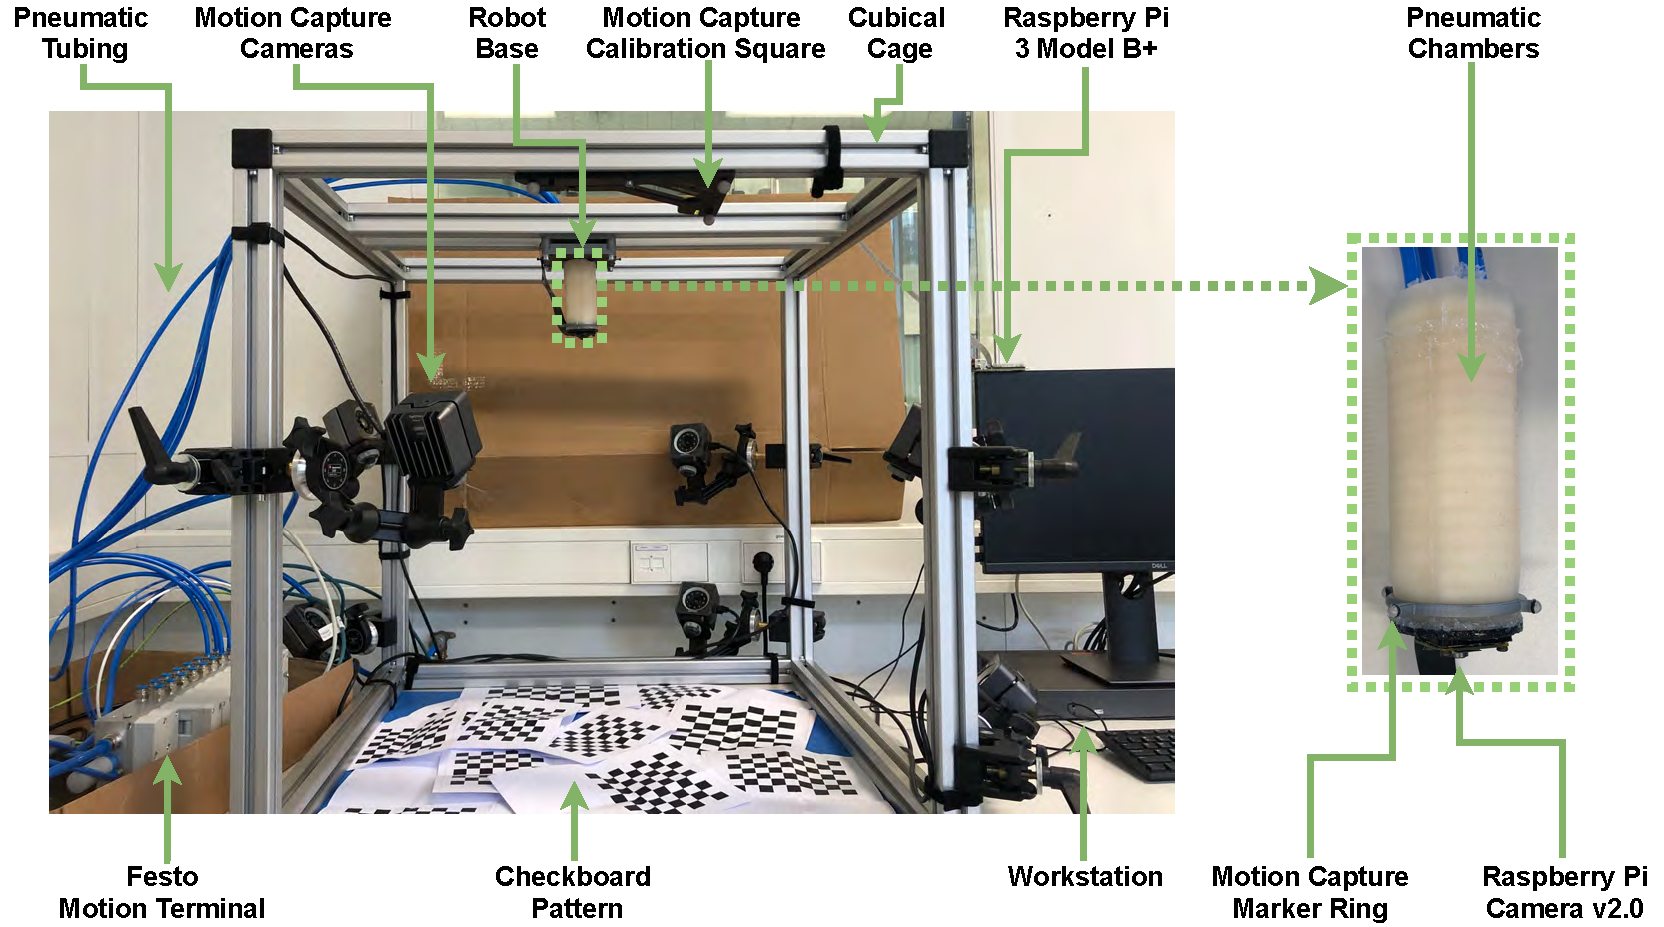
\includegraphics[height=.525\columnwidth]{srslam/figures/graphic_experimental_setup.drawio_v1_compressed.pdf} \label{fig:srslam:experimental_setup}}
     \subfigure[Trajectory 3]{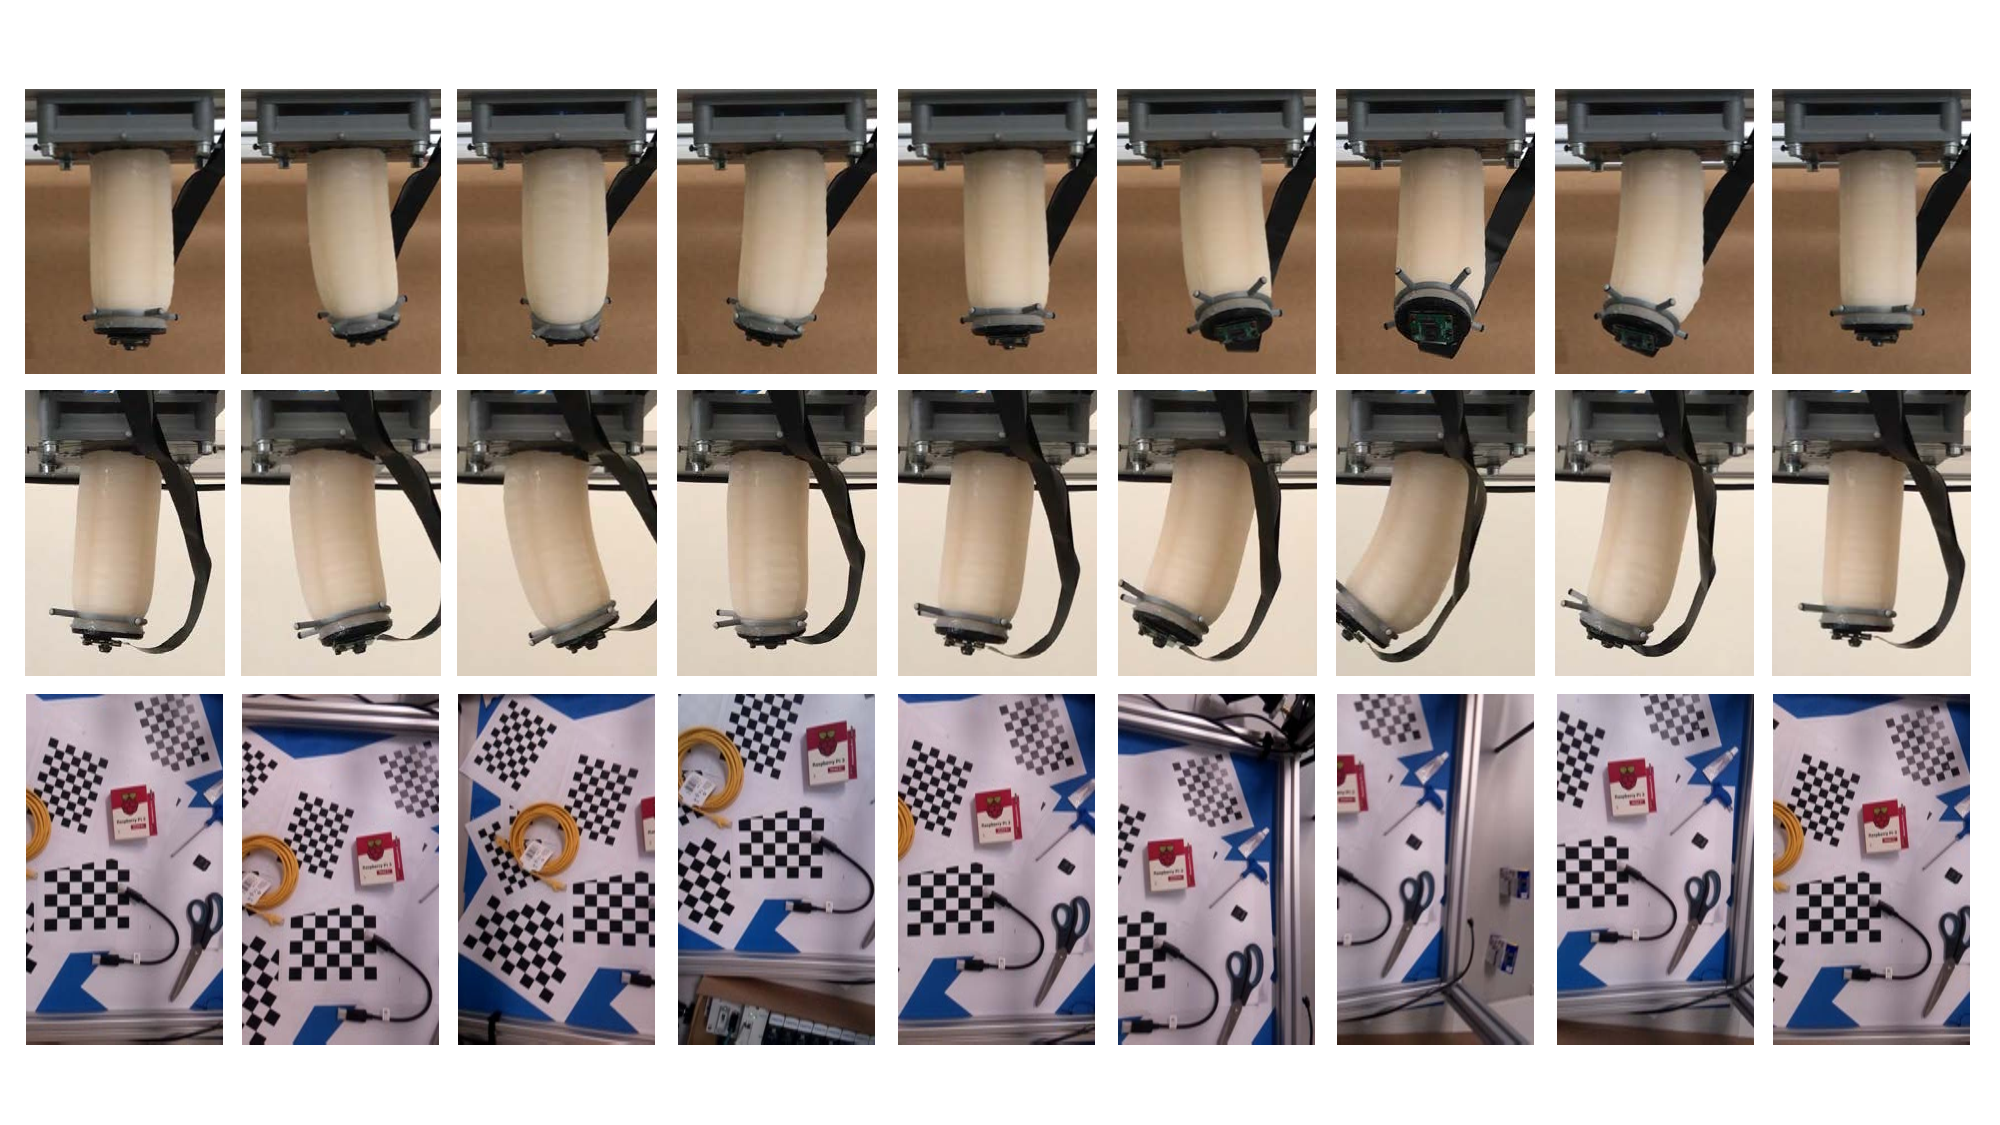
\includegraphics[height=.525\columnwidth]{srslam/figures/graphic_sequences_of_stills_lab_experiment_trajectory_3_compressed.pdf} \label{fig:srslam:graphic_sequences_of_stills_lab_experiment_trajectory_3}}
     \caption{ In Panel (a), a soft robotic segment is mounted to a cage with attached motion capture cameras. The segment is pneumatically actuated by a pressure regulator (Festo Motion Terminal). A Raspberry Pi camera v2.0 is attached to the tip of the segment and, in a straight segment configuration, looks down towards check-board patterns. Panel (b) depicts a sequence of stills showing the robot following trajectory 3 from two different vantage points. The second vantage point differs \SI{90}{\degree} from the first one. The third row displays a few representative frames, as recorded by the camera attached to the tip of the segment.}
\end{figure*}

\subsection{Experimental Setup}
% Segment and manufacturing
We show the experimental setup in Figure~\ref{fig:srslam:experimental_setup}.
We consider a soft robotic silicone segment consisting of four independently inflatable cavities. The segment has a cylindrical shape with a length $L_{0,1}$ of \SI{11}{cm} and a radius $d_1$ of \SI{21}{mm}. 
% We follow the fabrication procedure by \citet{marchese2015recipe} by casting Silicone into 3D-printed molds and block any silicon-flow into the air chambers with bees wax.
A 3D-printed ring with four motion capture markers is located near the tip of the segment.
%
% Camera and its attachment to the segment
We mount a Raspberry Pi camera module v2.0 to the tip of the segment.
This camera has a \SI{8}{MP} sensor and records frames at a sampling rate of \SI{30}{Hz} and a resolution of 1080p.
The focal length is \SI{3.04}{mm} and the field of view is $\SI{62.2}{\degree} \times \SI{48.8}{\degree}$.
The camera module is attached to a Raspberry Pi 3B+ single-board computer, which saves the frames for later processing by the ORB-SLAM~\citep{mur2017orb} algorithm.
The camera is screwed onto a custom 3D-printed holder, which in turn is glued with the tip plane of the segment.
%
% Actuation motion terminal, communication, commanding of pressures
The segment with its four air chambers is actuated with a proportional pressure regulator.
Tubing attached to the base of the segment connects each chamber with the assigned pneumatic valve of the pressure regulator.
%
% We apply a constant offset pressure $p_0$ to all chambers in straight configuration and subsequently synchronously increase the pressure $p_1$ in one chamber by $f_{\mathrm{p},x}$ and decrease the pressure in the opposite chamber $p_2$ by $f_{\mathrm{p},x}$ accordingly to cause a bending of the segment, in this case in x-direction.
% \begin{equation}
% \begin{split}
%     p_1 = p_0 - f_{\mathrm{p},x} \qquad p_2 = p_0 + f_{\mathrm{p},x}\\
%     p_3 = p_0 - f_{\mathrm{p},y} \qquad p_4 = p_0 + f_{\mathrm{p},y}
% \end{split}
% \end{equation}
% We map the desired configuration $\Delta_{x,1}$ and $\Delta_{y,1}$ given by the trajectories defined in \eqref{eq:srslam:trajectory_parametrization} in linear approximation to the commanded pressures
% \begin{equation}
%     f_{\mathrm{p},x} = a_x \; \Delta_{x,1} 
%     \qquad
%     f_{\mathrm{p},y} = a_y \; \Delta_{y,1}
%     \qquad
%     p_0 = a_{\delta L} \; \delta L_1
% \end{equation}
% where the proportional factors $a_{x}$, $a_{y}$ and $a_{\delta L}$ are experimentally determined and an elongation of the segment is reached through an increase in the offset pressure $p_0$.
% The pressure in each chamber is regulated by a Festo Motion Terminal using a factory-tuned PID controller.
% The commanded valve pressures are relayed via Modbus / TCP from our lab workstation to the Motion Terminal at a frequency of approximately \SI{10}{Hz}.
%
% Cage and environment
The segment is attached in an up-side-down configuration to the top plane of a cubical cage of \SI{750}{mm} side length. For a straight segment, the camera is facing downwards towards the floor of the cage, which is covered by multiple printed checkerboard patterns.
%
% Motion capture system and cage
We acquire ground-truth pose information of the tip of the segment using an Optitrack motion capture system. %, consisting of eight PrimeX 13 cameras mounted to the previously mentioned cubic cage. 
The ground-truth poses of the tip of the segment are recorded at \SI{30}{Hz}. % analogous to the Raspberry Pi camera frames.
% Additionally, we also record the pose of the base of the segment allowing us to determine a ground-truth coordinate transformation $T_{0}^{1}$ from the base to the tip.
%
% Implementation of PCC projection and calibration sequence
%In contrast to the model we used in simulation, the real-world segment experiences an elongation caused by the application of pressure to the chambers. Accordingly, 
%
We also include the elongation of the segment $\delta L_1$ in the cost function \eqref{eq:srslam:cost_fun} of our optimization.
%
% Calibration sequence
To resemble the calibration sequence from the simulation for the \gls{SLAM} map, we manually move the robot laterally into the x-coordinate direction before fixing it to the cage for the start of the experiments.

\subsection{Results}
Our experimental results reported in Table~\ref{tab:srslam:results_lab_experiments} and visualized for trajectory 3 in Figure~\ref{fig:srslam:experiments_t3_over_time} show translational relative \gls{RMSE} of between \SI{9}{\percent} and \SI{20}{\percent} for the three trajectories before optimization. 
The orientation of the z-axis of the tip is estimated with a mean error of approximately \SI{0.075}{\radian}.
The translational error is improved to between \SI{5}{\percent} and \SI{9}{\percent} after projection into the \gls{PCC}-kinematics. 
The optimization also slightly improves the rotational \gls{RMSE} by \SI{4}{\percent} to \SI{10}{\percent} relative to naive \gls{SLAM}.

The experimental results of the \gls{SLAM} algorithm are coherent with the simulations, as the small segment length (\SI{11}{cm}) used in the experiments increases the translational errors, as shown similarly in the simulations for a robot of length \SI{15}{cm}.
Even though the translational error is greatly reduced through optimization, it is still significantly higher than in simulation. Two reasons for this difference could be that a) the segment in the simulation was modeled as in-extensible, while the real robot segment is extended via pneumatic pressurization, which introduces additional errors by \gls{SLAM} not accurately estimating the elongation movement and b) the real robot does not perfectly behave according to the \gls{CC} approximation as the simulated robot does.

% \begin{table}
% \centering
% \caption{ \textcolor{orange}{OLD RESULTS: }oReal-world results before and after optimization: the translational errors are stated through a relative \gls{RMSE} and the rotational errors with an absolute \gls{RMSE} taking into account the Frobenius norm of the rotation matrices.}
% \begin{tabular}{lclll}\toprule
% \textbf{Error category} & \textbf{Opt.} & \textbf{Traj. 1} & \textbf{Traj. 2} & \textbf{Traj. 3}\\
% \midrule
% Translation $e_\mathrm{t}$ Eq.~\eqref{eq:srslam:evaluation_translational_error} & No & $\SI{24.8}{\percent}$ & $\SI{21.4}{\percent}$ & $\SI{9.5}{\percent}$ \\
% Translation $e_\mathrm{t}$ Eq.~\eqref{eq:srslam:evaluation_translational_error} & Yes & $\SI{11.4}{\percent}$ & $\SI{13.0}{\percent}$ & $\SI{4.5}{\percent}$ \\
% \midrule
% Rotation $e_\mathrm{R}$ Eq.~\eqref{eq:srslam:evaluation_rotational_error} & No & $0.105$ & $0.131$ & $0.116$ \\
% Rotation $e_\mathrm{R}$ Eq.~\eqref{eq:srslam:evaluation_rotational_error} & Yes & $0.098$ & $0.125$ & $0.112$ \\
% \midrule
% \textcolor{orange}{Rotation $e_{\theta_z}$ Eq.~\eqref{eq:srslam:evaluation_angle_error}} & No & $0.105$ & $0.131$ & $0.116$ \\
% \textcolor{orange}{Rotation $e_{\theta_z}$ Eq.~\eqref{eq:srslam:evaluation_angle_error}} & Yes & $0.098$ & $0.125$ & $0.112$ \\
% \bottomrule
% \end{tabular}
% \label{tab:srslam:results_lab_experiments}
% \end{table}

\begin{table}
\centering
\caption{ Real-world results before and after optimization. The translational errors are stated through a relative \gls{RMSE} as described in \eqref{eq:srslam:evaluation_translational_error}. For rotation, we report both an absolute \gls{RMSE} computed with the Frobenius norm between the rotation matrices as stated in \eqref{eq:srslam:evaluation_rotational_error} and an angle error [rad] for the orientation of the z-axis of the tip of the segment as defined in \eqref{eq:srslam:evaluation_angle_error}. The results are averaged over two trials for each trajectory.}
\begin{tabular}{lclll}\toprule
\textbf{Error category} & \textbf{Opt.} & \textbf{Traj. 1} & \textbf{Traj. 2} & \textbf{Traj. 3}\\
\midrule
Translation $e_\mathrm{t}$ & No & $\SI{20.3}{\percent}$ & $\SI{14.2}{\percent}$ & $\SI{9.1}{\percent}$ \\
Translation $e_\mathrm{t}$ & Yes & $\SI{9.1}{\percent}$ & $\SI{8.9}{\percent}$ & $\SI{5.0}{\percent}$ \\
\midrule
Rotation $e_\mathrm{R}$ & No & $0.145$ & $0.103$ & $0.126$ \\
Rotation $e_\mathrm{R}$ & Yes & $0.130$ & $0.099$ & $0.120$ \\
\midrule
Rotation $e_{\theta_z}$ & No & $\SI{0.079}{\radian}$ & $\SI{0.068}{\radian}$ & $\SI{0.084}{\radian}$ \\
Rotation $e_{\theta_z}$ & Yes & $\SI{0.080}{\radian}$ & $\SI{0.067}{\radian}$ & $\SI{0.084}{\radian}$ \\
\bottomrule
\end{tabular}
\label{tab:srslam:results_lab_experiments}
\end{table}

\begin{figure}[ht]
    \centering
    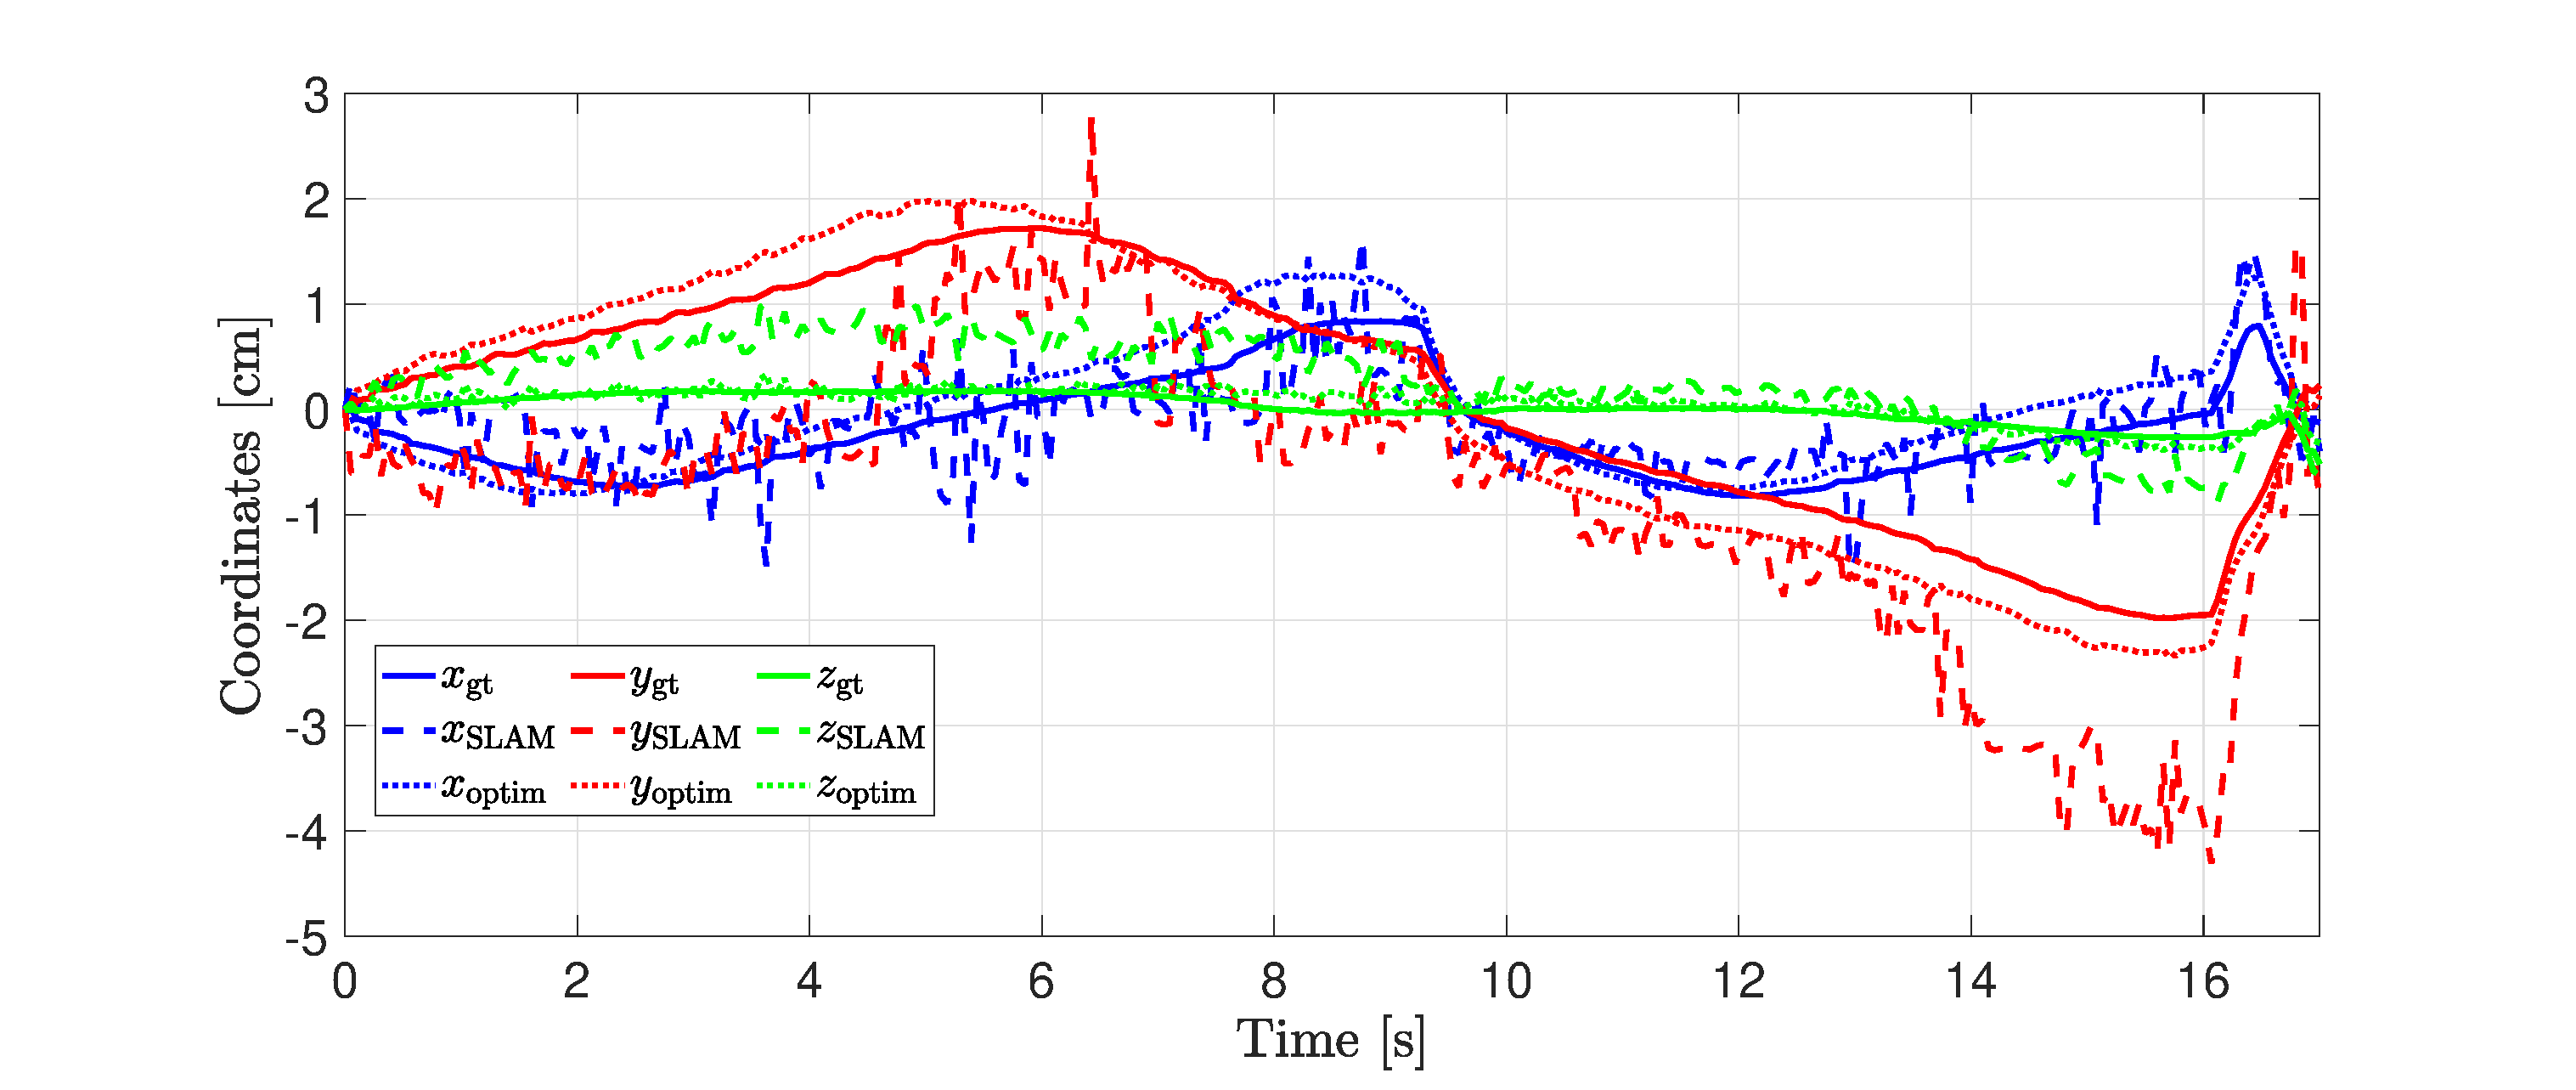
\includegraphics[width=0.9\columnwidth, trim={2cm 1.2cm 2cm 0}]{srslam/figures/vtem28_t3_coordinates.eps}\\
    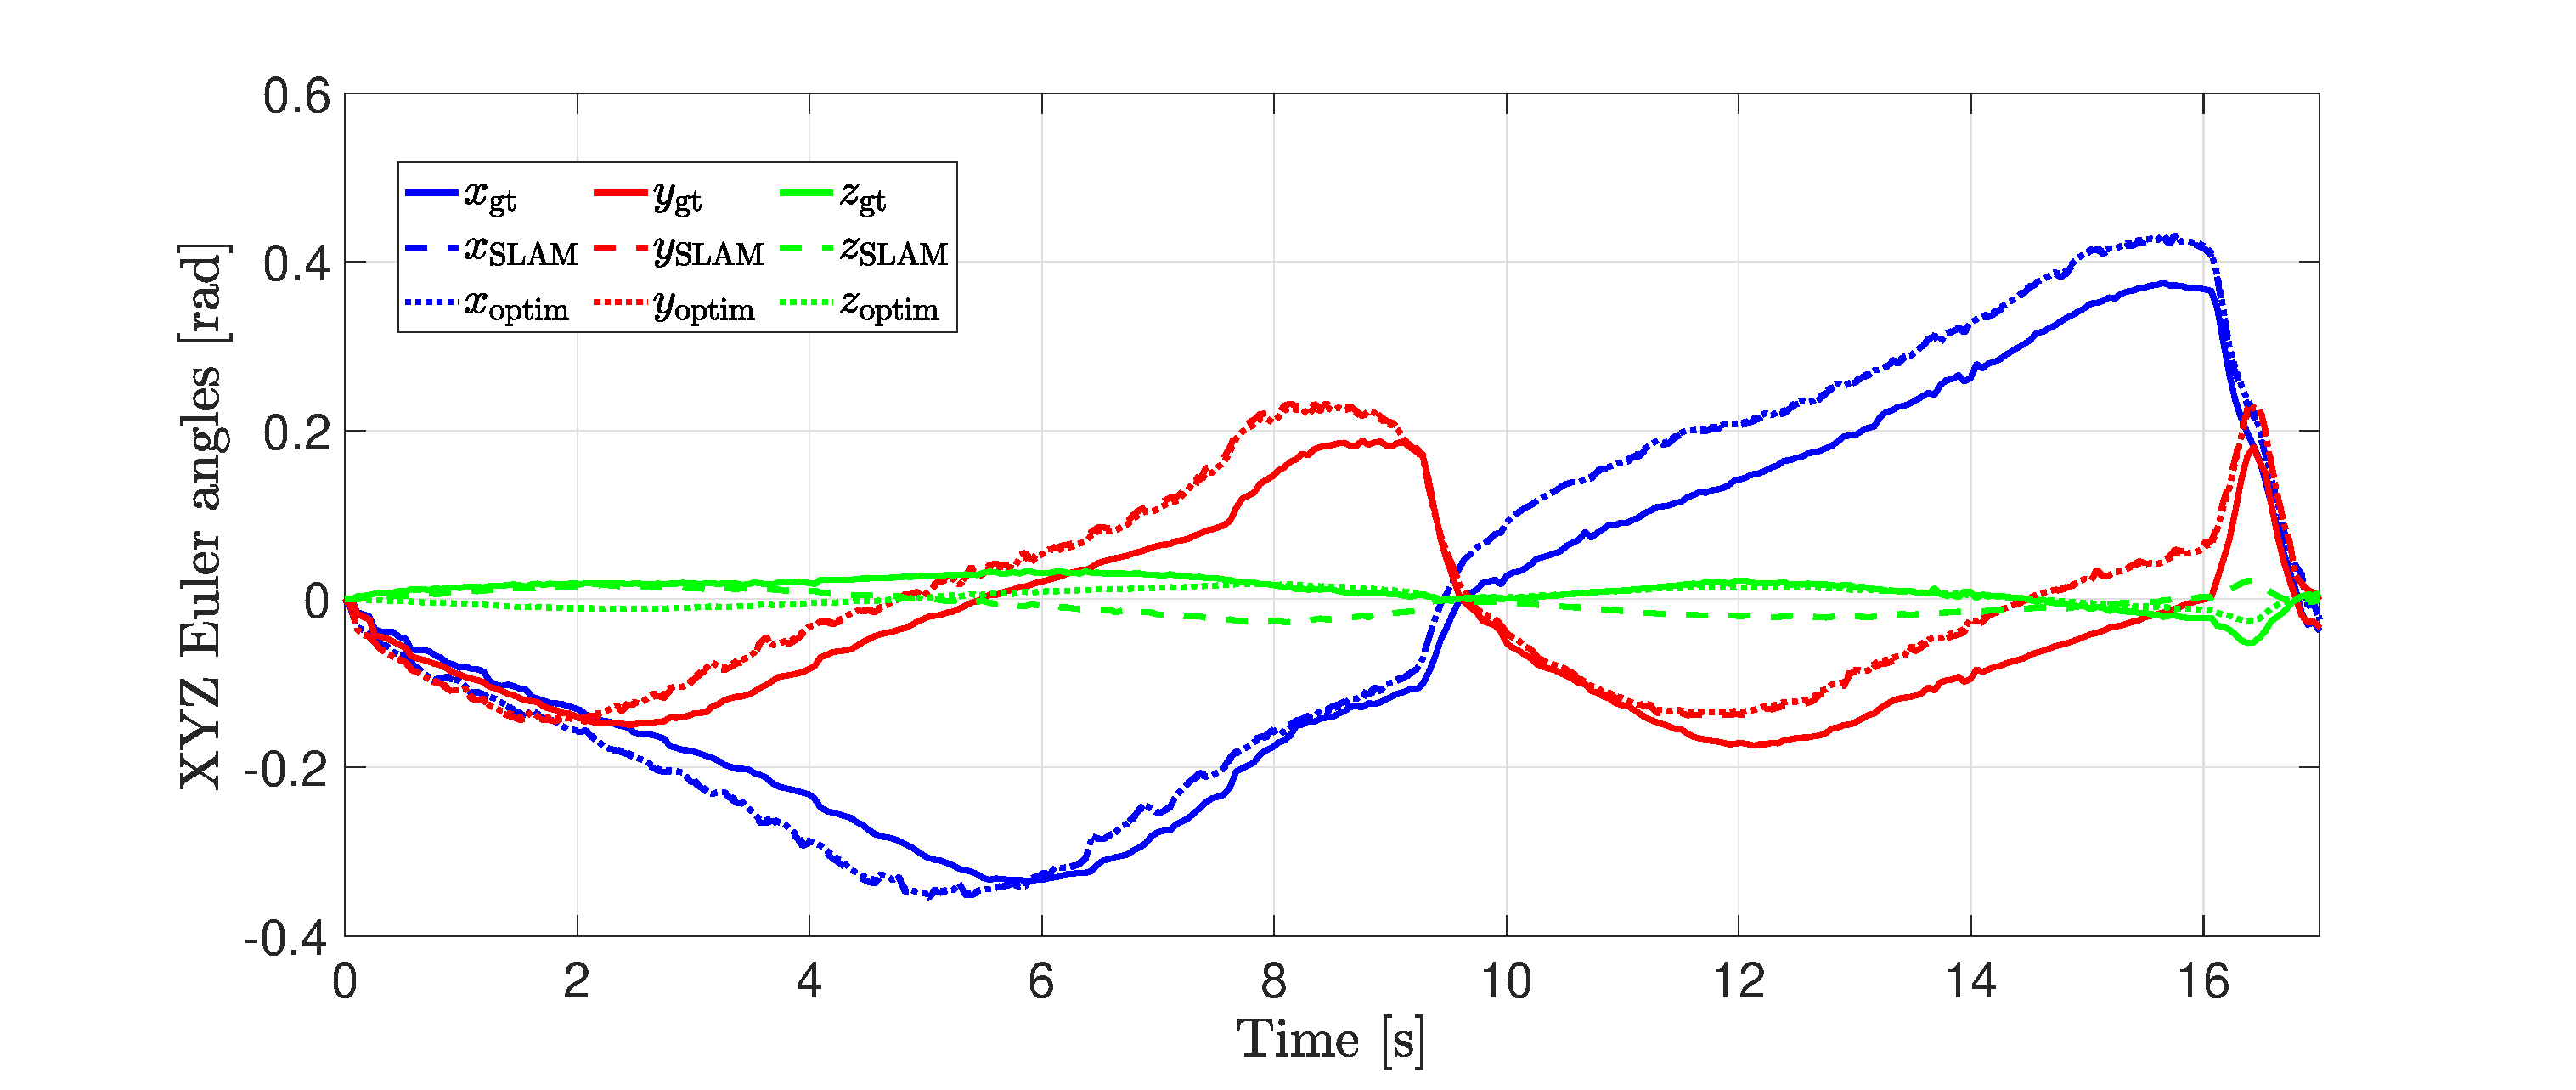
\includegraphics[width=0.9\columnwidth, trim={2cm 0 2cm 1.2cm}]{srslam/figures/vtem28_t3_angles.eps}
    \caption{ Experimental results for trajectory 3. Comparison between ground-truth (solid line), \gls{SLAM} (dashed line), and optimized through projection into \gls{PCC} kinematics (dotted line) for translation and orientation estimates.}
    \label{fig:srslam:experiments_t3_over_time}
\end{figure}


\section{Conclusion}
\label{sec:srslam:conclusions}

This paper investigated using a monocular camera in shape sensing of continuum soft robots, with the ultimate goal of implementing precise and reliable estimations at the cost of introducing small rigid parts into the hardware design. The contribution of this paper has been twofold. First, we proposed to use monocular SLAM with a soft robot. Second, we propose a regularization of the estimation based on a nonlinear projection in the manifold of admitted configuration. A nonlinear optimization implements the latter based on the kinematic model of the robot. We have performed extensive simulations with rendered images in Blender and lab experiments with a single segment soft robot. The nonlinear optimization based on the robot's kinematic model led to a significant improvement in translations and a marginal improvement in rotations. 
Future work will focus on extending the experimental validation of the method to multiple segments and cameras, bettering the SLAM by feeding back the kinematic projection in its state and using this estimation to implement closed-loop control.
While we conducted our experiments in a lab environment under ideal conditions with the camera pointed at checkerboard patterns thus resulting in plenty of image features for \gls{SLAM} to track, future work should investigate whether deployment environments for soft robots would be sufficiently feature-rich for the use of our proposed method.

\section*{Afterword}
This chapter demonstrated how inexpensive commercialized monocular cameras can be effectively used together with established \gls{SLAM} algorithms and kinematic models (e.g., \gls{PCC}) to achieve shape sensing for soft robots. One of the main advantages of this solution is that all necessary components are readily available - either commercially or even via open source. 
% Sharing the same vision, recent work by \citet{caroleo2025soft} combines commercial miniature \gls{TOF} sensors mounted to the tip of a segment with a particle filter for estimating the end-effector pose.
Sharing the same vision, recent work by \citet{caroleo2025soft} integrates commercial miniature \gls{TOF} sensors mounted at the segment tip with a particle filter to estimate the end-effector pose by considering the deviation from a known map of the environment.

However, the approach presented in this chapter also has some drawbacks: 
i) Firstly, while cameras have been significantly miniaturized in recent years, the requirement for them to have a clear, unobstructed view of the environment necessitates the inclusion of a rigid component on the surface of the soft robot, which we generally prefer to avoid for safety reasons. 
Secondly, ii), the performance of \gls{SLAM} algorithms is affected in environments with limited visually distinguishable features.
Finally, iii) high-dimensional perceptive data such as images are generally computationally expensive to process, leading to higher computational requirements and/or relatively low sampling rates of the shape-sensing information.
Therefore, we present in Chapter~\ref{chp:promasens} an alternative shape-sensing approach based on magnetic sensors. The necessary magnets and magnetic sensors can be deeply embedded into the soft robot body, thus allowing us to keep the robot surface entirely soft and compliant. Furthermore, the sensory data is several orders of magnitude lower dimensional, and thus, its processing is potentially much less computationally demanding.
% \chapter{Learning Proprioception for Continuum Soft Robots with Magnetic Sensors}
\chapter{Exploiting Learned Magnetic Fields and Kinematic Models for Shape Sensing}
\label{chp:promasens}

\begin{foreword}
    % Proprioception of its own state is a necessity for (soft) robots that enables many downstream applications such as control, motion planning, etc.
    % In Chapter~\ref{chp:srslam}, we presented an approach that executes kinematics-aware \gls{SLAM} on images from monocular cameras attached to the soft robot's body.
    % However, the presented approach also has some drawbacks: 
    % i) Firstly, while cameras have been significantly miniaturized in recent years, the requirement for them to have a clear, unobstructed view of the environment necessitates the inclusion of a rigid component on the surface of the soft robot, which we generally prefer to avoid for safety reasons. 
    % Secondly, ii), the performance of \gls{SLAM} algorithms is affected in environments with limited visually distinguishable features.
    % Finally, iii) high-dimensional perceptive data such as images are generally computationally expensive to process, leading to higher computational requirements and/or relatively low sampling rates of the shape-sensing information.
    % Therefore, we present in this chapter an alternative proprioception approach based on magnetic sensors. The necessary magnets and magnetic sensors can be deeply embedded into the soft robot body, thus allowing us to keep the robot surface entirely soft and compliant. Furthermore, the sensory data is several orders of magnitude lower dimensional, and thus, its processing is potentially much less computationally demanding.
    Proprioception is essential for (soft) robots, enabling applications like control and motion planning. In Chapter~\ref{chp:srslam}, we introduced a kinematics-aware \gls{SLAM} approach based on images from a monocular camera attached to the robot. However, this method has drawbacks: i) Cameras, despite their miniaturization, require a clear, unobstructed view, necessitating rigid components on the robot’s surface, which potentially compromises safety. ii) \gls{SLAM} algorithms perform poorly in environments with few visually distinguishable features. iii) Processing high-dimensional image data is computationally intensive, leading to higher processing demands and/or lower shape-sensing sampling rates. To address these issues, this chapter proposes an alternative proprioception method using magnetic sensors. These sensors, along with embedded magnets, can be fully integrated into the robot’s body, maintaining a soft, compliant surface. Additionally, the sensory data is much lower-dimensional, making it significantly less computationally demanding to process.
    However, the complex nature of magnetic fields makes the mapping from magnetic sensor readings to shape information very challenging, and it would be very hard to develop a fully physics-based model to help us interpret the sensor readings. Instead, we leverage modern \gls{ML} methods for this task.
    Akin to projecting the \gls{SLAM} pose measurements onto the kinematic model (Chapter~\ref{chp:srslam}), we again leverage here kinematic knowledge to simplify the problem setting. 
    Specifically, instead of learning proprioception end-to-end from magnetic sensor measurements to configuration values, we simplify the learning problem by asking a neural network to predict the measurements of a sensor given a parametrization of the spatial relation between the magnetic sensor and all magnets embedded in the robot. We present the proposed methodology in detail in Sec.~\ref{sec:promasens:methodology}.
    We verify the proposed approach extensively in simulations based on \gls{PCC}- \& \gls{PAC}-parametrized soft robots (Section~\ref{sec:promasens:pcc_simulations} \& \ref{sec:promasens:ac_simulations}), and experimentally in Section~\ref{sec:promasens:experiments} on a one-segment soft robot moving in 3D space.
\end{foreword}


\pagebreak

\begin{abstract}
    Sensing the shape of continuum soft robots without obstructing their movements and modifying their natural softness requires innovative solutions. This chapter proposes to use magnetic sensors that are fully integrated into the robot to achieve proprioception. Magnetic sensors are compact, sensitive, and easy to integrate into a soft robot. We also propose a neural architecture to make sense of the highly nonlinear relationship between the perceived intensity of the magnetic field and the shape of the robot. By injecting a priori knowledge from the kinematic model, we obtain an effective yet data-efficient learning strategy. We first demonstrate in simulation the value of this kinematic prior by investigating the proprioception behavior when varying the sensor configuration, which does not require us to re-train the neural network. We validate our approach in experiments involving one soft segment containing a cylindrical magnet and three magnetoresistive sensors. During the experiments, we achieve mean relative errors of 4.5\%.
\end{abstract}

\blfootnote{This chapter is partly based on \faFileTextO~\emph{T. Baaij*, M. K. Holkenborg*, \textbf{M. Stölzle}*, D. van der Tuin*, J. Naaktgeboren, R. Babuška, and C. Della Santina (2023). Learning 3D shape proprioception for continuum soft robots with multiple magnetic sensors. Soft Matter, 19(1), 44-56}~\citep{baaij2023learning}.

% \nth{1}-author contributions: M. Stölzle conceived and implemented the methodology, conducted all simulations, and wrote the paper. T. Baaij, M. K. Holkenborg, and D. van der Tuin developed the physical soft segment prototype, which included a strategy for embedding sensors and magnets into the robot and a pipeline for processing the experimental data.
T.B., M.K.H., M.S., and D.v.d.T contributed equally to this chapter. 
C.D.S. and R.B. conceived and led the project. M.S. invented the proprioception algorithm and implemented all simulations. T.B., M.K.H., J.N., and D.v.d.T designed the strategy to integrate sensors and magnets into the robot. T.B., M.K.H., J.N., and D.v.d.T developed the PCB and sensing electronics. T.B., M.K.H., and D.v.d.T fabricated the soft robot. T.B., M.K.H., J.N., and D.v.d.T implemented the experimental data processing pipeline. T.B., M.K.H., M.S., and D.v.d.T conducted experiments. T.B., M.K.H., M.S., and D.v.d.T tuned the learning strategy and developed suitable trajectories. T.B., M.K.H., M.S., and D.v.d.T wrote the manuscript. C.D.S. and R.B. revised the manuscript.
}

%% Start the actual chapter on a new page.
\newpage

\section{Introduction}\label{sec:promasens:introduction}
%
%Driven by the aim of building robots that can safely interact with complex and fragile environments,
%
The past decade has seen an explosion of novel continuum soft robotic platforms \cite{luong2019eversion,shah2021soft,hughes2020extensible}. Inspired by invertebrate animals, these robots are almost entirely composed of soft deformable materials \cite{della2021soft}. This makes them robust and safe, but at the same time, it renders their modeling \cite{armanini2021soft}, control \cite{della2023model}, and shape sensing \cite{wang2018toward} substantially more complex than for their rigid counterparts.
%
Shape sensing is especially complex because it is both a technological and algorithmic challenge. Sensors must not obstruct the natural behavior or reduce the compliance of soft robots. At the same time, non-collocated and nonlinear sensors require algorithms for the measurements to be interpreted and connected to a description of the robot's shape.

Several sensing modalities have been considered to implement shape sensing, such as resistive~\cite{shih2019design, kramer2011soft}, capacitive~\cite{scimeca2019model, shintake2018ultrastretchable}, optical~\cite{li2021scaling}, and visual~\cite{rosi2022sensing}. Magnetic sensors~\cite{song2015electromagnetic, ozel2015precise, luo2017toward, guo2019continuum, mitchell2021fast} are a promising solution. Magnetic sensors are compact, highly sensitive, and can be easily integrated into existing soft robot designs. Thus, they can provide reliable and fully proprioceptive measurements at the cost of a minimal decrease in the robot's softness. Among the above-cited papers, the only work leveraging external magnetic fields is by Song et al.~\cite{song2015electromagnetic}, where coils placed at a distance generate the magnetic field.
Along this thought, an obvious choice would be to measure the earth's magnetic field for proprioception purposes. However, it would only allow estimating two rotational components, and any translational effects, such as an elongation of the continuum robot, could not be captured.
%\textcolor{blue}{Since a soft robot will elongate when pneumatically actuated, it is required to quantify the lengthening or shortening of the robot. This can not be achieved with solely an constant external magnetic source (like earth) and thus, an permanent magnet needs to be embedded in the robot.} 
Alternatively, some papers \cite{ozel2015precise,luo2017toward,guo2019continuum} use co-axial pairs of magnets and sensors embedded in the robot to estimate planar deformations. Recently, Mitchell et al.~\cite{mitchell2021fast} have shown that a similar strategy can sense 3D deformations. Such simple arrangements greatly simplify the analysis, allowing for connecting readings to shape through direct interpolation. Nevertheless, relying on isolated pairs of sensors and magnets also strongly limits the density and the amount of information gathered through this method.

% \begin{figure*}[ht]
%   \centering
%   \includegraphics[width=1.0\textwidth]{promasens/figures/methodology/methodology_proprioception_v6_compressed.pdf}
%   \caption{Proprioception for continuum soft robots with magnetic sensors: an initial \gls{PCC} configuration estimate $\hat{q} \in \mathbb{R}^{n_\mathrm{b}}$ is employed to derive the kinematic relationship between a sensor and each magnet. Subsequently, this kinematic description is used to predict the sensor measurements $\hat{u} \in \mathbb{R}^{n_\mathrm{s}}$ through a previously trained neural network. A \gls{MSE} error metric evaluates the accuracy of the predictions compared to the actual measurements $u$. Finally, we optimize the configuration estimate $\hat{q}$ to achieve proprioception by minimizing the sensor measurement prediction loss.}
%   \label{fig:promasens:methodology}
% \end{figure*}

\begin{figure*}[ht]
  \centering
  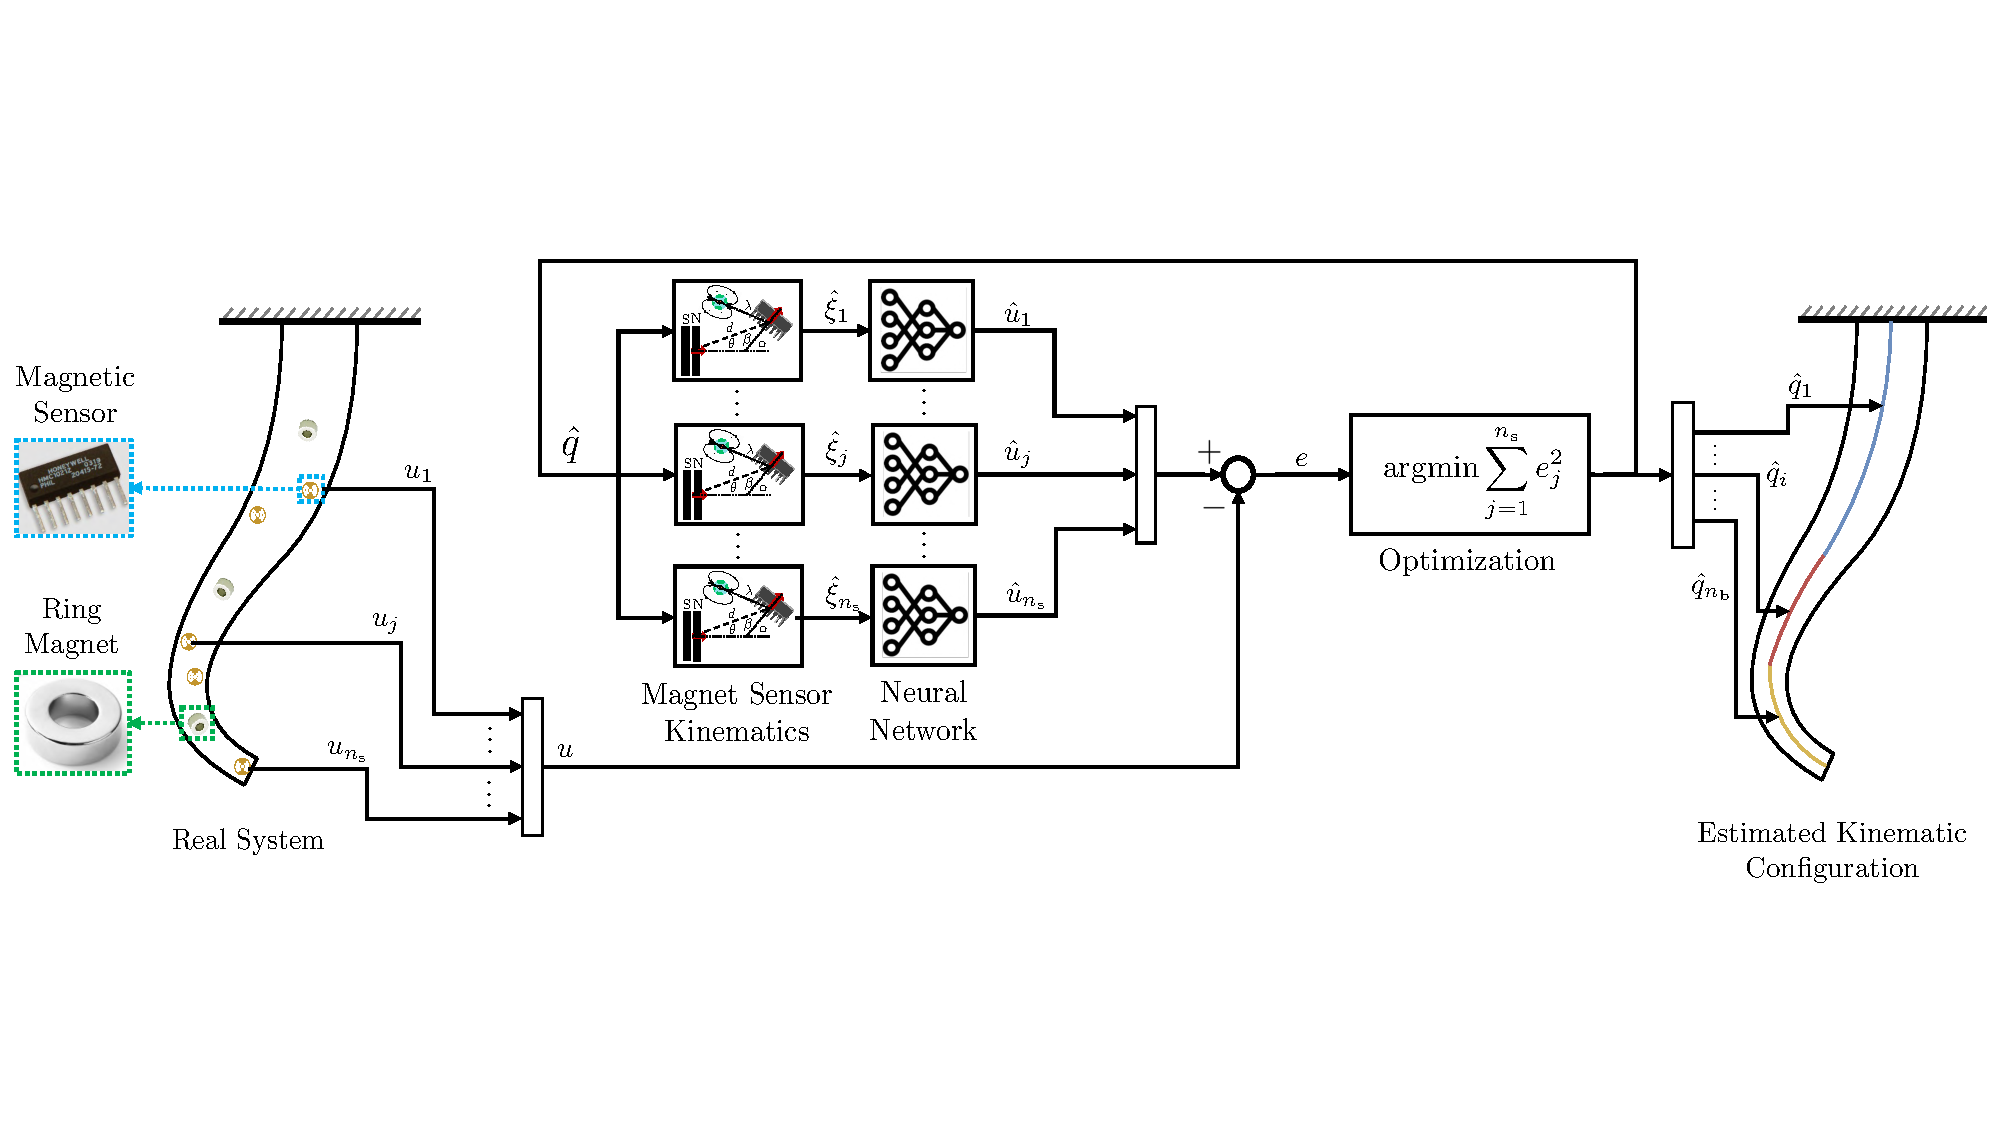
\includegraphics[width=1.0\textwidth]{promasens/figures/methodology/methodology_proprioception_v8_compressed.pdf}
  
  \caption{Proprioception for continuum soft robots with magnetic sensors: an initial configuration estimate $\hat{q}$ is employed to derive the kinematic relationship $\hat{\xi}$ between a sensor and each magnet. Subsequently, this kinematic description is used to predict the sensor measurements $\hat{u} \in \mathbb{R}^{n_\mathrm{s}}$ with a neural network trained in advance. A Mean Squared Error (MSE) metric evaluates the accuracy of the predictions $\hat{u}$ compared to the actual measurements $u$. Finally, we optimize the configuration estimate $\hat{q}$ to achieve proprioception by minimizing the sensor measurement prediction loss.}\label{fig:promasens:methodology}
\end{figure*}

% However, the physical interaction between magnets, sensors, the earth's magnetic field and external disturbances is very complex and highly nonlinear.

% This means that simplified analytical models are usually not sufficient~\cite{ozel2015precise} and inverting the magnetic field equations directly to match sensor measurements with relative locations of the magnet and sensor is intractable~\cite{mitchell2021fast}.

% Related research published by H. Gao et al.~\cite{guo2019continuum} consider a continuum robot made-up of many small sections each containing a magnet and a magnetic sensor. Their approach relies on an analytical model to estimate the 1D bending of small sections of a continuum robot. Subsequently, they fit Quadratic Bézier curves to the curvature of each section to model the shape of the continuum robot.

% An alternative to inaccurate analytical models is to conduct FEA simulations of the magnetic field for the chosen robot design and sensor layout~\cite{ozel2015precise, mitchell2021fast}.

% S. Ozel et al.~\cite{ozel2015precise} leverage Hall effect sensors to measure the curvature of a soft snake-like robot in 2D with both the sensor and magnet directly embedded in the silicon. They rely on data from FEA simulations stored in a look-up table to connect the measured magnetic flux density to translations relative to the magnet. A calibration function derived with least-squares fitting connects the relative translations to the soft robot curvature.

% Along a similar line of work, Mitchell et al.~\cite{mitchell2021fast} follow a probabilistic approach by implementing a particle filter for proprioception with a tri-axis Hall effect sensor. The likelihood weight of each particle is given by the proximity of simulated magnetic flux measurements to the actual measurements.

% All existing approaches rely either on simplified analytical models, which are not suitable for complex geometric arrangements between magnets and sensors, or require to mirror the robot design with all necessary (DoF) in a simulator.

This paper proposes to use permanent ring magnets and multiple magnetic sensors for shape sensing of continuum soft robots. Importantly, we remove the requirement of magnets and sensors being placed in co-axial pairs.
% placed at arbitrary locations within the soft segment. We then present a data-driven approach for making sense of the complex relationship between  measurements - so achieving proprioception with magnetic sensors.
%
We have been inspired by recent work leveraging deep learning to interpret various types of non-magnetic sensor data for proprioception purposes~\cite{truby2020distributed, ding2021predictive, soter2018bodily, thuruthel2019soft}.
% All of them except one~\cite{ding2021predictive} choose Recurrent Neural Network (RNN) structures as their neural network architecture to encourage temporal consistency of the robots' state estimates.
%
However, learning end-to-end mappings from sensors to configurations has three significant drawbacks: (i) it is data-intensive, (ii) it calls for recurrent architectures to encourage temporal consistency for the robot's configuration estimates, (iii) it requires re-training when changing the kinematic model of the robot. We propose a neural architecture that circumvents all three issues (see Fig. \ref{fig:promasens:methodology}).
First, we train shallow neural networks to predict the measurements of the magnetic sensors from a parameterization describing their relative pose with respect to the magnets. We then optimize the configuration estimate - and thus the sensor positions - to minimize the error between the predicted and actual sensor measurements. 
% The result is the robot configuration estimate that better explains the sensor readings. 
This way, we introduce a priori information on the modes of deformation of a continuum soft robot, effectively removing the kinematics from the black box. 
The presented strategy enables us to re-arrange and remove redundant sensors during inference without requiring us to re-train the neural network on the adjusted sensor configuration.
% We provide experiments showing that this architecture achieves a mean precision of \SI{95.5}{\percent} when applied to 3D shape proprioception of a soft segment. 
% Testing on a similar trajectory type as trained on, even an error as low as \SI{1.4}{\percent} is possible.

% However, these existing solutions have some possible drawbacks~\cite{wang2018toward}. The piezoresistive and optical sensors are based over the entire length of the robot. This might result into issues with the robustness of these sensors when the robot has to deform more than the stretchability of the sensors allow. This issue could be resolved with Hall effect sensors, since there is no physical connection between the magnet and the sensor that restricts the robots motion. However, previous papers exploring the use of Hall effect sensors did not consider the estimation of 3D state parametrization.
% %
% This paper proposes a kinematically decoupled, data-driven approach for achieving proprioception with magnetic sensors. We assume the placement of a permanent magnet at the center and multiple magnetoresistive sensors at arbitrary locations within the soft segment.
% Subsequently, we model the kinematic relationship between each magnet and sensor.
% This allows us to remove the kinematics from the black-box and train a neural network to predict the sensor measurements based on a very flexible input description independent of the used state parametrization of the robot.
% An advantage of this explicit kinematic description is that the position of a sensor or magnet can be changed without re-training the entire black-box if the neural network is trained on a sufficient large dataset of kinematic descriptions.
% We employ a loss between the predicted and actual sensor measurements to guide a nonlinear optimization strategy to compute the robot configuration estimate.
% The optimization approach consists of grid search running at lower frequencies in parallel to a fast gradient descent algorithm for local corrections.

% \textcolor{orange}{Do we hypothesize that this reduces the number of trainable parameters?}

% This paper will explore the option to use \gls{MRS} and a permanent magnet, to find a relation between the \gls{MRS} output ans the sensor's position relative to the magnet. Due to the non-linearity of magnetic fields, it is hard to predict this relationship as found in previous 2D applications of similar sensors. Therefore, this paper will look at using \gls{AI} to experimentally link the \gls{MRS} output to a 3D position.
%
% First, a model is needed that captures the position and movement of the robot. For this robot, the \gls{PCC} model is used~\cite{della2020improved}. Subsequently, this model can be used to find the parameters that physically relate the relative position of the magnet and the sensor, the \gls{MSK}. This will be used in combination with a \gls{NN} to predict the sensory output of a single sensor. Afterwards, the error between the predicted sensor output and the measured output is taken. By introducing multiple sensors, a gradient descent can be implemented to descent to the robots configuration by minimizing the error between the predicted and measured sensor values.

To summarize, this paper contributes to the state of the art in soft robot sensing with:
%
\begin{itemize}
    \item A proprioceptive sensing modality relying on multiple magnetic sensors in conjunction with a neural network-based architecture that learns to estimate the full 3D shape of the robot from the sensor readings. % The strategy can deal with small training sets thanks to the injection of kinematic priors.
    % \item A data-driven approach to predict the measurements of \glsp{MRS} integrated into a multi-segment soft robot.
    \item Injection of kinematic priors through a description to spatially relate the poses of a sensor to the magnets. This proposed description serves as an input to a neural network predicting the sensor measurements. %This kinematic description can be easily derived from the \gls{PCC} state description by providing the initial position of magnets and sensors in a straight robot configuration.
    % \item An optimization routine for minimizing the sensor prediction error by running a slow grid search and fast gradient descent in parallel.
    \item Experimental verification of the approach for a one-segment robot with three integrated Magnetoresistive Sensors (MRSs) and proprioception of 3D curvature.    % \item A robust data-driven approach to achieve proprioception for a multi-segment, soft, snake-like robot in 3D.
    %\item Variable and scalable approach to \gls{MRS} measurements.
    % \item Combination of a data-driven sensor measurement model and \gls{MSK} in a gradient descent approach for proprioception.
    % \item Proposing a design how permanent magnets and \glsp{MRS} can be easily integrated into a soft robot.
\end{itemize}
We open-source a Python / PyTorch implementation of the proposed algorithm and the corresponding datasets on GitHub~\footnote{\url{https://www.github.com/tud-cor-sr/promasens}}.

% \begin{figure}[ht]
%     \centering
%     \includegraphics[width=0.575\columnwidth]{promasens/figures/methodology/kinematic_frames_v3_cropped.pdf}
%     \caption{Coordinate frames for a soft segment containing the $j^\mathrm{th}$ magnetic sensor and the $k^\mathrm{th}$ cylindrical magnet placed along the center line. $\{S_{i-1}\}$ and $\{S_{i}\}$ describe the frames of the base and tip of the $i^\mathrm{th}$ segment respectively.}\label{fig:promasens:kinematics_frames_soft_segment}
% \end{figure}

\section{Proprioception with Magnetic Sensors}

This section introduces a methodology to achieve proprioception for soft robots with magnetic sensors.
%
We consider a continuum robot with the shape of its backbone described by the configuration variables $q \in \mathbb{R}^{n_\mathrm{q}}$.
In the commonly used \gls{PCC} kinematic state parametrization~\cite{webster2010design}, the continuum robot is assumed to consist of $n_\mathrm{b}$ segments with each segment exhibiting constant curvature and elongation along its length. Therefore, the configuration of the soft robot can be described with $q \in \mathbb{R}^{3n_\mathrm{b}}$.
Please refer to Appendix~\ref{sub:promasens:kinematic_model_pcc} for more details.
We indeed use PCC for most of our simulations and experiments.
Note, however, that the proposed proprioception algorithm applies to any finite-dimensional kinematic description of a soft robot~\cite{armanini2021soft}.
Indeed, we also specifically consider a robot with affine curvature~\cite{della2020soft, stella2022piecewise_preprint} with its shape described by the configuration $q \in \mathbb{R}^4$. We document this alternative kinematic model in Appendix~\ref{sub:promasens:kinematic_model_ac}.
The proprioception methodology described in the remaining section is agnostic to the chosen kinematic model.
% For the sake of clarity, we use the \gls{PCC} kinematic state parametrization as proposed by \cite{della2020improved}. We consider a continuum robot described by $n_\mathrm{b}$ \gls{CC} segments and configuration variables $q \in \mathbb{R}^{3n_\mathrm{b}}$. Note, however, that the proposed method applies to any finite-dimensional kinematic description of a soft robot~\cite{armanini2021soft}.

\subsection{Proposed method at a glance}

%The shape of each segment can be parameterized with $q_i$.
We integrate $n_\mathrm{m}$ axially symmetric magnets and $n_\mathrm{s}$ magnetic sensors into the robot. The magnets must be installed along the center line of the segment while the sensors can be arbitrarily placed.
%
%To achieve proprioception of the entire robot shape, at least one magnet must be integrated into each segment.
%
Fig.~\ref{fig:promasens:methodology} concisely describes the proposed shape-sensing strategy with a pictorial example of a soft robot described with three constant curvature segments equipped with five magnetic sensors and three cylindrical magnets.
%

The goal of the algorithmic part (center of the figure) is to regress the robot shape (left) by estimating the configuration $\hat{q}$ of all segments (right),
%$q(t) \in \mathbb{R}^{3 n_\mathrm{b}}$
starting from the measurements of the magnetic sensors $u$ (e.g. usually the magnetic flux density).
We achieve this by training a sensor measurement predictor and subsequently optimizing the configuration estimate $\hat{q}$ for the prediction $\hat{u}$ to match the actual sensor measurement $u$.
Instead of predicting the sensor measurements end-to-end, we decouple the kinematics by explicitly describing the kinematic relationship $\hat{\xi}_j = f_{\xi,j}(\hat{q})$ between sensor $j$ and each magnet. % \hat{\xi}_j \in \mathbb{R}^{1+4 n_\mathrm{m}}
Then, we train a neural network $f_{\pi_j}$ to predict the measurement $\hat{u}_j$ based on the input $\hat{\xi}_j$.
To achieve proprioception, we jointly optimize $\hat{q}$ for all sensor measurement predictions. %We define a \gls{MSE} loss between the predicted and actual sensor measurements, and after back-propagating the loss, we perform gradient descent.

% PCC Kinematics with Elongation
% \subsection{Background: Piecewise Constant Curvature Kinematics}\label{sub:promasens:kinematic_model_pcc}

% The state of each segment $i$ of unextended length $L_{0,i}$ and radius $d_i$ is described by
% \begin{equation}\small
%     q_i = \begin{bmatrix}\Delta_{x,i} & \Delta_{y,i} & \delta L_i \end{bmatrix}^{\mathrm{T}} \in \mathbb{R}^3
% \end{equation}
% where $\Delta_{x,i}$ and $\Delta_{y,i}$ represent bending into the local x- and y-directions respectively and $\delta L_i$ defines the extension of the segment.
% The base frame of segment $i$ is referred to as $\{S_{i-1}\}$ as stated in Fig.~\ref{fig:promasens:kinematics_frames_soft_segment}. Given $q_i$, a homogeneous transformation $T_{i-1}^{i}(q_i)$ to the tip frame $\{S_{i}\}$ is available
% \begin{equation}\small
% \label{eq:promasens:transform_improved_q}
% \begin{split}
%     R_{i-1}^{i} &=
%     \begin{bmatrix}
%         1 + \frac{\Delta_{x,i}^2}{\Delta_{i}^2} \left ( \mathrm{c}_i - 1 \right ) & \frac{\Delta_{x,i} \Delta_{y,i}}{\Delta_{i}^2} \left ( \mathrm{c}_i - 1 \right ) & \frac{\Delta_{x,i}}{\Delta_i} \mathrm{s}_i\\
%         \frac{\Delta_{x,i} \Delta_{y,i}}{\Delta_{i}^2} \left ( \mathrm{c}_i - 1 \right ) & 1 + \frac{\Delta_{y,i}^2}{\Delta_{i}^2} \left ( \mathrm{c}_i - 1 \right ) & \frac{\Delta_{y,i}}{\Delta_i} \mathrm{s}_i\\
%         \frac{-\Delta_{x,i}}{\Delta_i} \mathrm{s}_i & \frac{-\Delta_{y,i}}{\Delta_i} \mathrm{s}_i & \mathrm{c}_i
%     \end{bmatrix},\\
%     t_{i-1}^{i} &= \frac{d_i ( L_{0,i}+\delta L_i)}{\Delta_i^2}
%     \begin{bmatrix}
%         \Delta_{x,i} (1 - \mathrm{c}_i) & \Delta_{y,i} (1 - \mathrm{c}_i) & \Delta_{i} \mathrm{s}_i,
%     \end{bmatrix}^{\mathrm{T}}
% \end{split}
% \end{equation}
% where we substituted $\Delta_i = \sqrt{\Delta_{x,i}^2 + \Delta_{y,i}^2}$, $\mathrm{s}_i = \sin \left ( \frac{\Delta_i}{d_i} \right )$, and $\mathrm{c}_i = \cos \left ( \frac{\Delta_i}{d_i} \right )$ for conciseness.

\begin{figure}[t]
\centering
\subfigure[Magnet Sensor Kinematics]{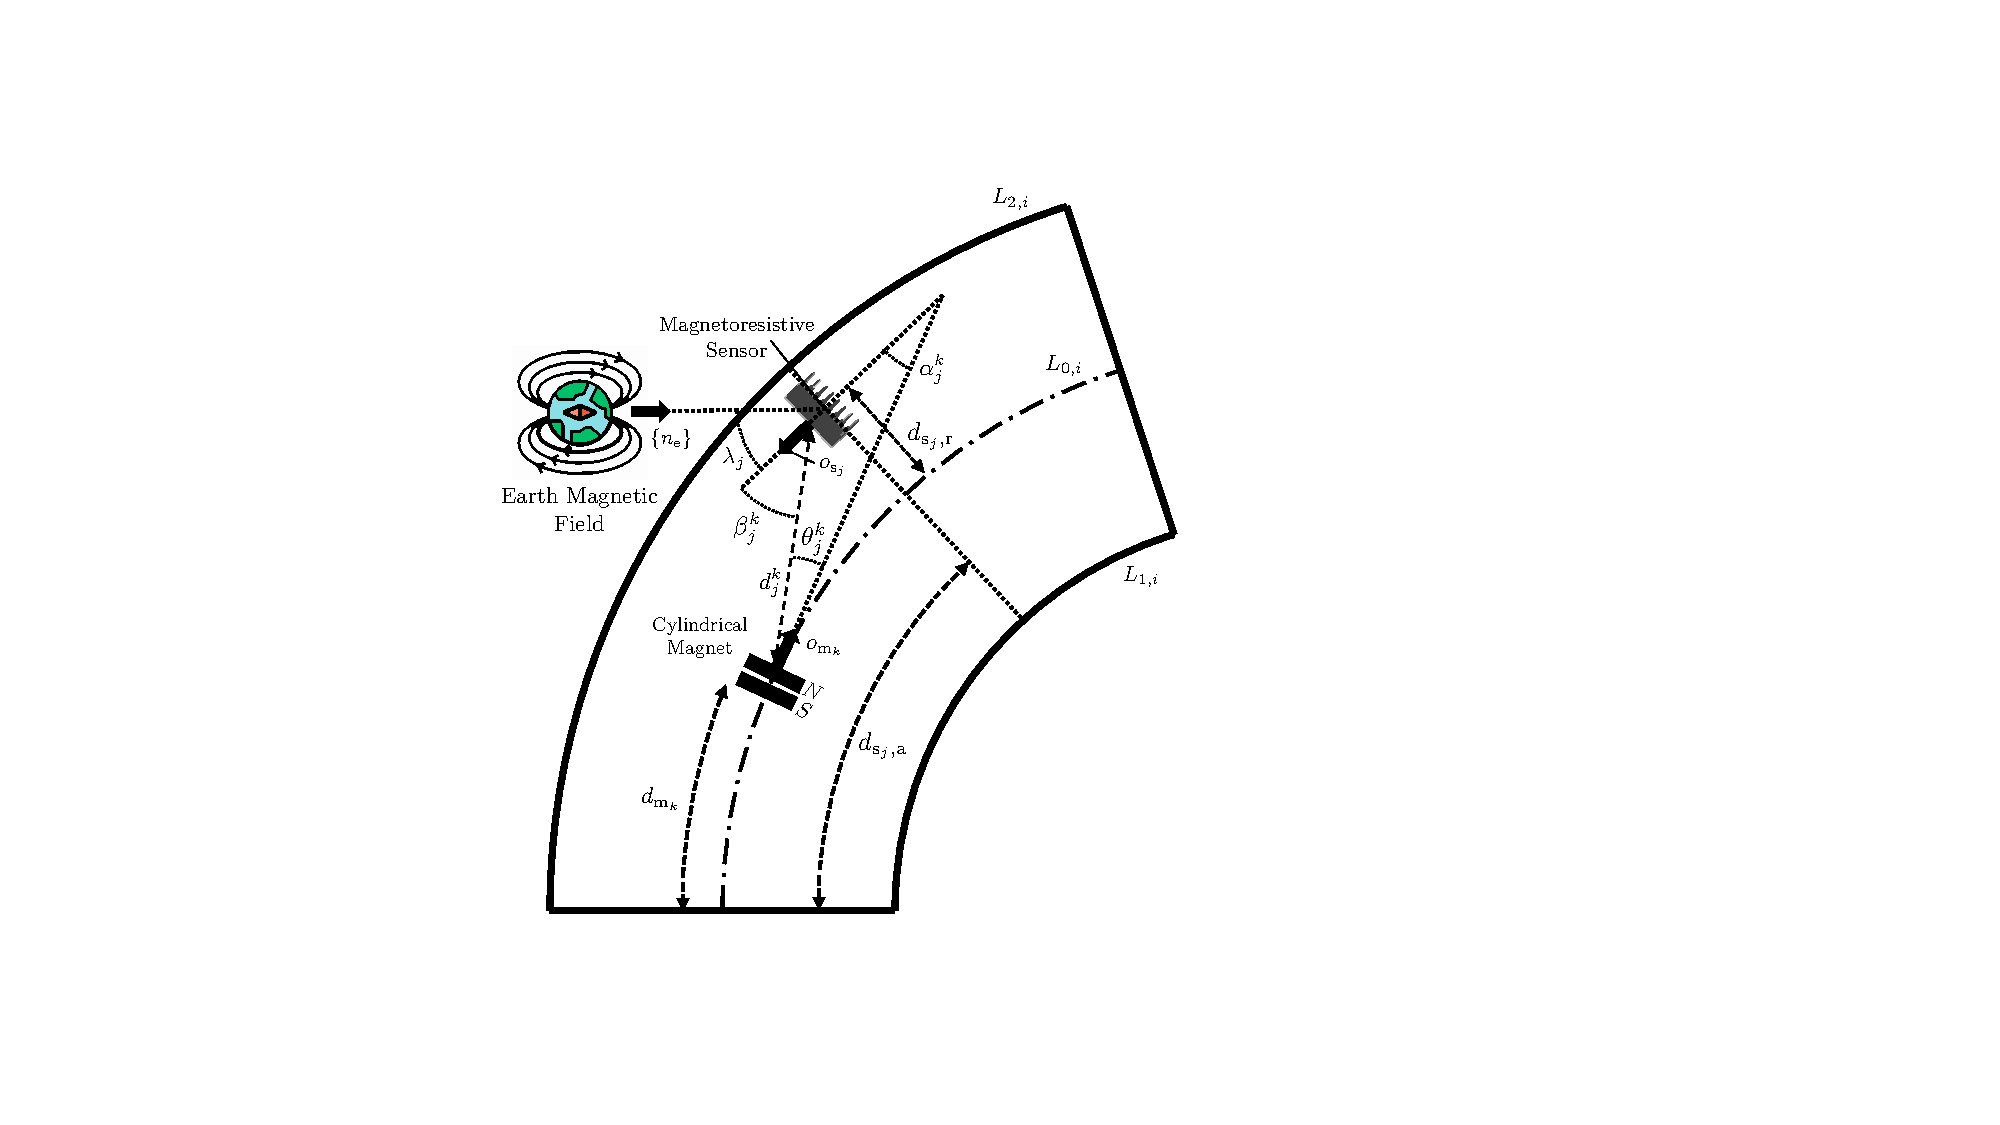
\includegraphics[width=0.5\columnwidth]{promasens/figures/methodology/magnet_sensor_kinematics_v5_compressed.pdf}\label{fig:promasens:magnet_sensor_kinematic}}
\subfigure[Coordinate transformations]{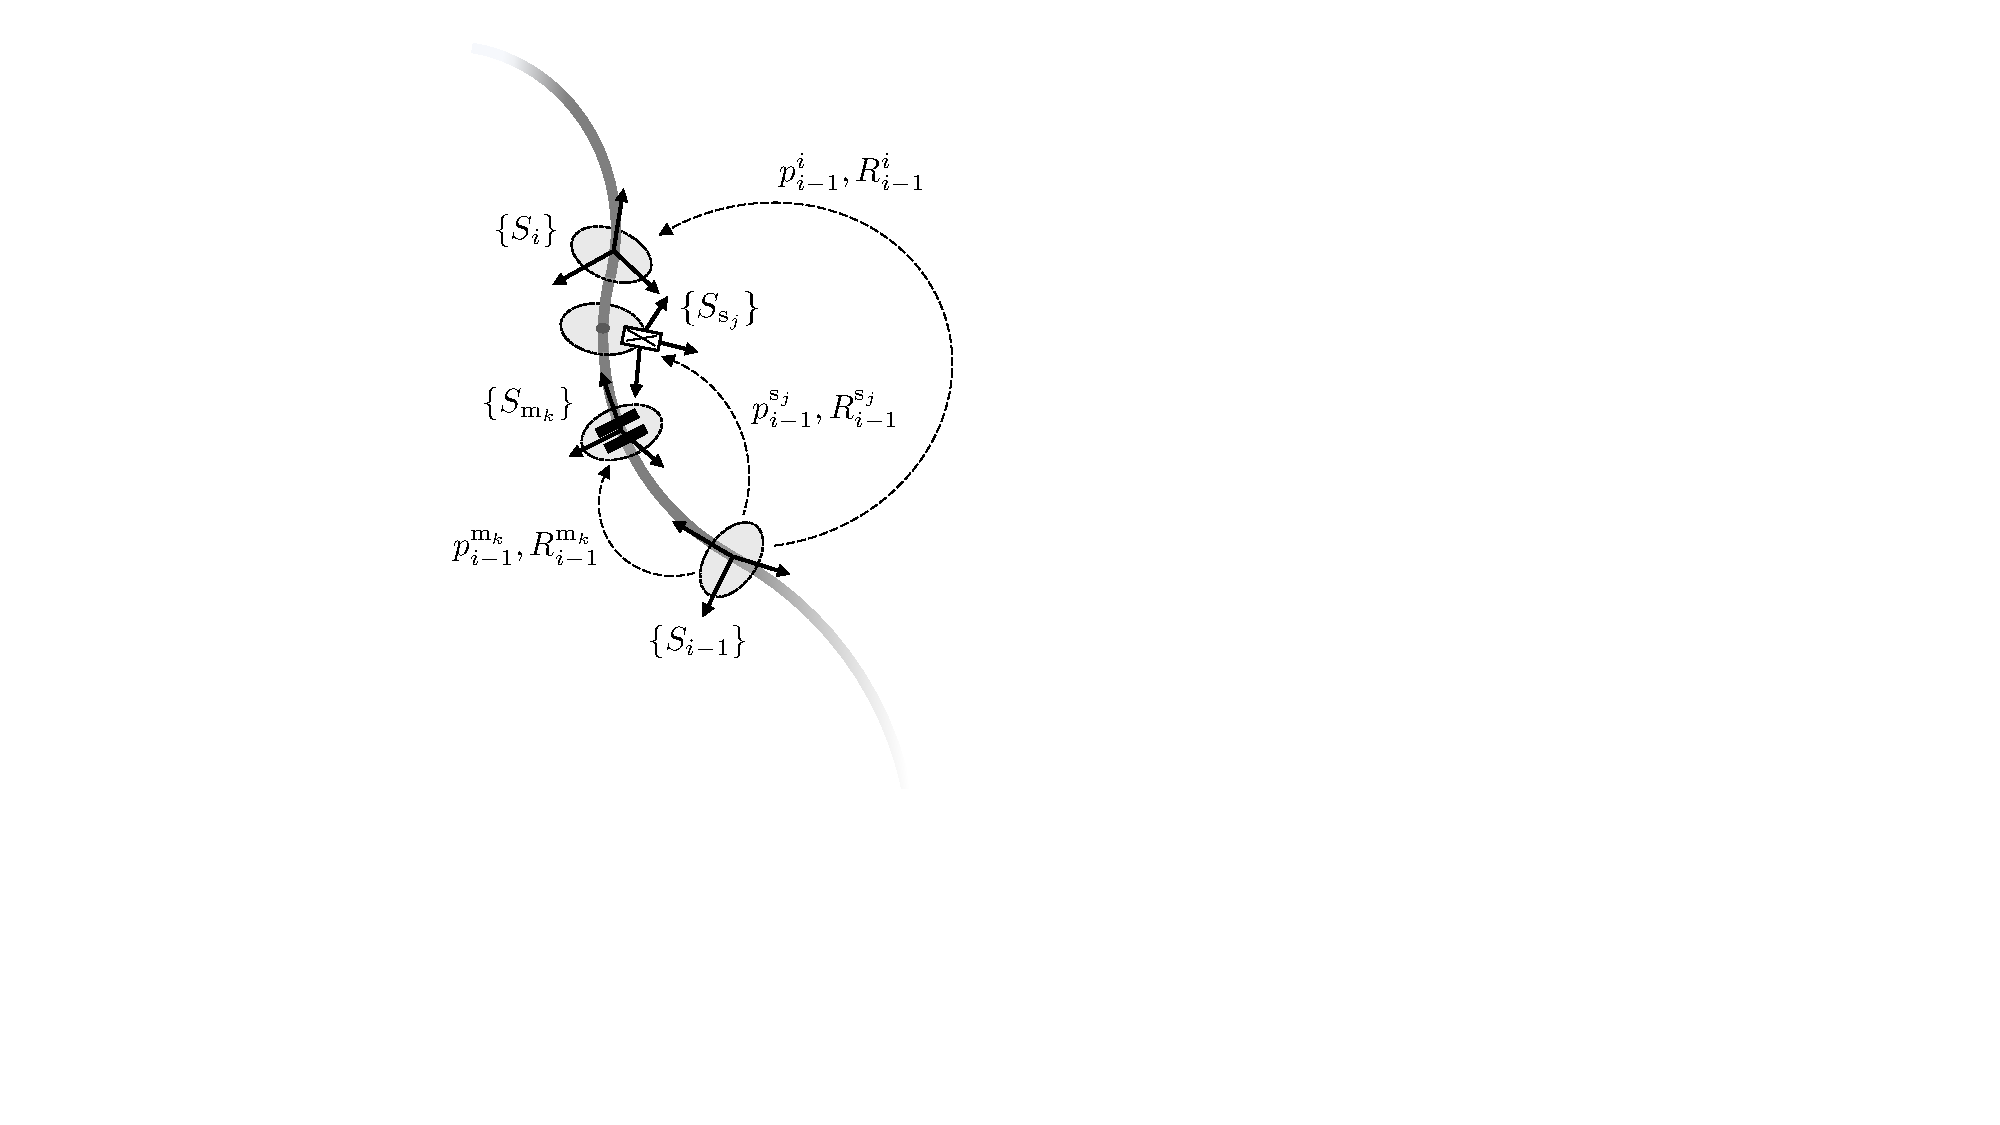
\includegraphics[width=0.4\columnwidth]{promasens/figures/methodology/kinematic_frames_v5_cropped.pdf}\label{fig:promasens:kinematics_frames_soft_segment}}
\caption{\textbf{Panel (a):} Parameters used to describe the kinematics between the $j^\mathrm{th}$ sensor and the $k^\mathrm{th}$ magnet. To simplify the illustration, we visualize the unextended planar case with both magnet and sensor part of the $i^\mathrm{th}$ segment. However, this is not a strict assumption as magnets and sensors can also be part of different segments. \textbf{Panel (b):} Coordinate frames for a soft segment containing the $j^\mathrm{th}$ magnetoresistive sensor and the $k^\mathrm{th}$ cylindrical magnet placed along the center line. $\{S_{i-1}\}$ and $\{S_{i}\}$ describe the frames of the base and tip of the $i^\mathrm{th}$ segment, respectively.}
\end{figure}

\section{Background: Continuum soft robot kinematics}\label{sec:promasens:kinematics}
A kinematic description provides us with the forward kinematic transformation $T_{i-1}^s(q_i,s)$ from base frame $\{S_{i-1}\}$ at the proximal end of the $i^\mathrm{th}$ segment to the local frame $\{S_{v}\}$ at a coordinate $v \in [0,1]$ for a given configuration $q_i$. Furthermore, the tip frame of the $i^\mathrm{th}$ segment located at the coordinate $v = 1$ is denoted as $\{S_{i}\}$, as shown in Fig.~\ref{fig:promasens:kinematics_frames_soft_segment}.

\subsection{$\Delta$-parametrization of the piecewise constant curvature kinematics}\label{sub:promasens:kinematic_model_pcc}
% \section*{Appendix: $\Delta$-parametrization of the Piecewise Constant Curvature Kinematics}\label{sub:promasens:kinematic_model_pcc}

Under the \gls{PCC} hypothesis, the shape of each segment $i$ of length $L_{i}$ and radius $d_i$ can be fully parameterized through three variables
\begin{equation}\small
    q_i = \begin{bmatrix}\Delta_{x,i} & \Delta_{y,i} & \delta L_{i} \end{bmatrix}^{\mathrm{T}} \in \mathbb{R}^3
\end{equation}
where $\Delta_{x,i}$ and $\Delta_{y,i}$ represent bending into the local $x$ and $y$ directions respectively and $\delta L_i$ defines the elongation of the segment.
The base frame of segment $i$ is referred to as $\{S_{i-1}\}$ as stated in Fig.~\ref{fig:promasens:kinematics_frames_soft_segment}. Given $q_i$, a homogeneous transformation $T_{i-1}^{v}(q_i, v)$ to the point frame $\{S_{v}\}$ is available
\begin{equation}\small
\label{eq:promasens:transform_improved_q}
\begin{split}
    R_{i-1}^{v}(q_i,v) &=
    \begin{bmatrix}
        1 + \frac{\Delta_{x,i}^2}{\Delta_{i}^2} \left ( \mathrm{C}_v - 1 \right ) & \frac{\Delta_{x,i} \Delta_{y,i}}{\Delta_{i}^2} \left ( \mathrm{C}_v - 1 \right ) & \frac{\Delta_{x,i}}{\Delta_i} \mathrm{S}_v\\
        \frac{\Delta_{x,i} \Delta_{y,i}}{\Delta_{i}^2} \left ( \mathrm{C}_v - 1 \right ) & 1 + \frac{\Delta_{y,i}^2}{\Delta_{i}^2} \left ( \mathrm{C}_v - 1 \right ) & \frac{\Delta_{y,i}}{\Delta_i} \mathrm{S}_v\\
        \frac{-\Delta_{x,i}}{\Delta_i} \mathrm{S}_v & \frac{-\Delta_{y,i}}{\Delta_i} \mathrm{S}_v & \mathrm{C}_v
    \end{bmatrix},\\
    p_{i-1}^{i}(q_i,v) &= \frac{d_i ( L_{0,i}+\delta L_i)}{v \, \Delta_i^2}
    \begin{bmatrix}
        \Delta_{x,i} (1 - \mathrm{C}_v) & \Delta_{y,i} (1 - \mathrm{C}_v) & \Delta_{i} \mathrm{S}_v,
    \end{bmatrix}^{\mathrm{T}}
\end{split}
\end{equation}
where $R_{i-1}^{v}$, $p_{i-1}^{i}(q_i,v)$ denote the rotation matrix and translation vector respectively. We substituted $\Delta_i = \sqrt{\Delta_{x,i}^2 + \Delta_{y,i}^2}$, $\mathrm{S}_v = \sin \left (\frac{v \, \Delta_i}{d_i} \right )$, and $\mathrm{C}_v = \cos \left ( \frac{v \, \Delta_i}{d_i} \right )$ for conciseness.

\subsection{Affine curvature kinematics}\label{sub:promasens:kinematic_model_ac}
The affine curvature hypothesis~\cite{della2020soft, stella2022piecewise_preprint} models the bending of the soft segment to be conforming to the affine function $\kappa(t,v) = \kappa_0(t) + \kappa_1(t) v$, where $\kappa$ describes the local curvature of the backbone at the coordinate $v \in [0, 1]$ along the segment and $\kappa_0(t)$, $\kappa_1(t)$ are the zero-order and first-order term of the curvature polynomial respectively~\cite{della2019control}.
Specifically, we implement the recently proposed extension to 3D environments~\cite{stella2022piecewise_preprint}, which specifies an azimuth angle of the bending direction $\phi(t)$ and additionally allows for an elongation $\delta L(t)$ of the segment.
% We extend this parametrization as introduced by Della Santina et al.~\cite{della2019control, della2020soft} to 3D environments by specifying the azimuth angle of the bending direction $\phi(t)$ and additionally allowing for an elongation $\delta L(t)$ of the segment. 
Accordingly, the configuration of the $i^\mathrm{th}$ segment is described at any point in time by
\begin{equation}\small
    q_i = \begin{bmatrix}\kappa_{0,i} & \kappa_{1,i} & \phi_i & \delta L_{i} \end{bmatrix}^{\mathrm{T}} \in \mathbb{R}^4.
\end{equation}
Now that the configuration space is defined, we aim to find a description of the forward kinematics. Firstly, the bending angle $\theta_i(q, v)$ is found by integrating the curvature
\begin{equation}\small
    \theta(q,v) = \int_{v'=0}^{v} \kappa_i(q, v') \, \mathrm{d}v' = \kappa_{0,i} \, v + \kappa_{1,i} \, \frac{v^2}{2}.
\end{equation}
The rotation to the frame $\{S_{v}\}$ can then be easily determined with $R_{i-1}^{i}(q,v) = R_{\phi_i}(q,v) \, R_{\theta}(q,v) R_{\phi_i}^\mathrm{T}(q,v)$. After substituting $S_{\cdot} = \sin(\cdot)$, $C_{\cdot} = \cos(\cdot)$ for conciseness, we state the homogeneous transformation as
\begin{equation}\small\label{eq:promasens:affine_curvature_forward_kinematics}
\begin{split}
    R_{i-1}^v(q,v) &= \begin{bmatrix}
        S_{\phi_i}^2 C_{\theta_v} + C_{\phi_i}^2 & -S_{\phi_i} C_{\phi_i} C_{\theta_i} + S_{\phi_i}C_{\phi_i} & S_{\phi_i} S_{\theta_v}\\
        -S_{\phi_i} C_{\phi_i} C_{\theta_i} + S_{\phi_i} C_{\phi_i} & S_{\phi_i}^2 + C_{\phi_i}^2 C_{\theta_v} & -S_{\theta_v} C_{\phi_i}\\
        -S_{\phi_i} S_{\theta_v} & S_{\theta_v} C_{\phi_i} & C_{\theta_i}
    \end{bmatrix},\\
    p_{i-1}^{v}(q,v) &= \left ( L_{0,i} + \delta L_i \right ) \, \begin{pmatrix}
        \int_{v'=0}^{v} \sin(\theta(q, v')) \, \mathrm{d}v' \, \sin(\phi_i)\\
        - \int_{v'=0}^{v} \sin(\theta(q, v')) \, \mathrm{d}v' \, \cos(\phi_i)\\
        \int_{v'=0}^{v} \cos(\theta(q, v')) \, \mathrm{d}v'
    \end{pmatrix}.
\end{split}
\end{equation}
We choose to integrate the translational terms in \eqref{eq:promasens:affine_curvature_forward_kinematics} numerically with $101$ sample points using the Torchquad~\cite{gomez2021torchquad} implementation of the Simpson's rule, which makes the forward kinematics fully and automatically differentiable.


\subsection{Magnet sensor kinematics}\label{sub:promasens:kinematic_model_magnet_sensor_kinematics}
This subsection derives the kinematic relationship $\xi_j = f_{\xi_j}(q) \in \mathbb{R}^{1+4n_\mathrm{m}}$ between the $j^\mathrm{th}$ sensor and all $n_\mathrm{m}$ magnets as we hypothesize that we can estimate the sensor measurement $u_j$ solely based on
a) the angle $\lambda_j \in \mathbb{R}^1$ to the earth's magnetic field,
b) the distance $d_j^k$  between the $j^\mathrm{th}$ sensor and $k^\mathrm{th}$ magnet,
c) the angle $\alpha_j^k$ between the sensor measurement direction and the cylindrical axis of the magnet,
d) the angle $\beta_j^k$ between the sensor measurement direction and the vector from the magnet to the sensor,
and e) the angle $\theta_j^k$ between the cylindrical axis of the magnet and the vector from the magnet to the sensor.
Accordingly, $\xi_j$ is defined as
\begin{equation}\small
    \xi_{j} = f_{\mathrm{\xi},j}(q) =
    \begin{pmatrix}
        \lambda_{j} & {\xi_{j}^1}^\mathrm{T} & \cdots & {\xi_{j}^k}^\mathrm{T} & \cdots & {\xi_{j}^{n_\mathrm{m}}}^\mathrm{T}
    \end{pmatrix}^\mathrm{T} \in \mathbb{R}^{1 + 4n_\mathrm{m}},
\end{equation}
with $\xi_j^{k} \in \mathbb{R}^4$ the kinematic relationship between the $j^\mathrm{th}$ sensor and the $k^\mathrm{th}$ magnet: $\xi_j^{k} = \begin{pmatrix} d_j^k & \alpha_j^k & \beta_j^k & \theta_j^k \end{pmatrix}^\mathrm{T} \in \mathbb{R}^4$. We visualize the parameters incorporated in $\xi_j^{k}$ in Fig.~\ref{fig:promasens:magnet_sensor_kinematic}.
% \begin{equation}\small
%     \xi_j^{k} = \begin{pmatrix} d_j^k & \alpha_j^k & \beta_j^k & \theta_j^k \end{pmatrix}^\mathrm{T}.
% \end{equation}

In the following, we present the derivation of all components of $\xi_j^{k}$. 
Please note that all kinematic frames used in the following paragraphs are visualized in Fig.~\ref{fig:promasens:kinematics_frames_soft_segment}.
% \textcolor{blue}{All the kinematic frames introduced over the last few paragraphs are visualized in Fig.~\ref{fig:promasens:kinematics_frames_soft_segment}}.

We define that the $k^\mathrm{th}$ magnet is integrated into the $i^\mathrm{th}$ segment. Now, we first derive a transformation matrix $T_{i-1}^{\mathrm{m}_k}$ from the base frame $\{S_{i-1}\}$ to the magnet frame $\{ S_{\mathrm{m}_k} \}$. 
This can be achieved by evaluating the chosen kinematic model, two of which we report in the Appendix~\ref{appx:kinematics}, at the segment coordinate $v = \frac{d_{\mathrm{m}_k}}{L_{0,i}}$. 
This means that the cylindrical magnet is integrated at a distance, which is measured along the backbone, of $d_{\mathrm{m}_k}$ from the base of the segment.
% The cylindrical magnet is integrated into the segment at an axial distance of $d_{\mathrm{m}_k}$ from $\{S_{i-1}\}$.
% We compute the translational and rotational components of the transformation matrix $p_{i-1}^{\mathrm{m}_k}$ and $R_{i-1}^{\mathrm{m}_k}$ \textcolor{blue}{by evaluating the forward kinematics $T_{i-1}^v(q_i,v)$, which are reported in Appendix~\ref{appx:kinematics}, at the point $v = \frac{d_{\mathrm{m}_k}}{L_{0,i}}$.}

% as in \cite{della2020improved} by substituting $\Delta_{x}^{\mathrm{m}_k} = \frac{d_{\mathrm{m}_k}}{L_{0,i}} \, \Delta_{x,i}$, $\Delta_{y}^{\mathrm{m}_k} = \frac{d_{\mathrm{m}_k}}{L_{0,i}} \, \Delta_{y,i}$ and $\Delta_{\mathrm{m}_k} = \frac{d_{\mathrm{m}_k}}{L_{0,i}} \, \Delta_{i}$. % in \eqref{eq:promasens:transform_improved_q}.

Subsequently, we  describe the pose of the $j^\mathrm{th}$ sensor with respect to the base of the $i^\mathrm{th}$ segment.
Denote with $d_{\mathrm{s}_j,\mathrm{r}}$ the radial distance of the sensor from the center line, with $\varphi_j$ the azimuth angle of the sensor in the cylindrical plane, and with $d_{\mathrm{s}_j,\mathrm{a}}$ the axial distance along the center line from the base of the $i^\mathrm{th}$ segment.
We derive the transformation $T_{i-1}^{\mathrm{s}_j,\mathrm{r}_0}$ to the center of the cylindrical plane of the sensor % using \eqref{eq:promasens:transform_improved_q}
analogously as for the magnets by evaluating the forward kinematics at $v = \frac{d_{\mathrm{s}_j,\mathrm{a}}}{L_{0,i}}$.
% by scaling the configuration vector $q_i$ with $\frac{d_{\mathrm{s}_j,\mathrm{a}}}{L_{0,i}}$ in the transformation matrix~\cite{della2020improved}.
This is followed by applying the radial offset $d_{\mathrm{s}_j,\mathrm{r}}$ in the cylindrical plane of the sensor
% \begin{equation}\small
% \begin{split}
%     t_{i-1}^{\mathrm{s}_j} = t_{i-1}^{\mathrm{s}_j,\mathrm{r}_0} + R_{i-1}^{\mathrm{s}_j,\mathrm{r}_0} \, d_{\mathrm{s}_j,\mathrm{r}}
%     \,
%     \begin{pmatrix}
%         \cos{\varphi_j} & \sin{\varphi_j} & 0
%     \end{pmatrix}^{\mathrm{T}}.
% \end{split}
% \end{equation}
\begin{equation}\small
    T_{i-1}^{\mathrm{s}_j} = T_{i-1}^{\mathrm{s}_j,\mathrm{r}_0}
    \,
    \begin{bmatrix}
        \cos{\varphi_j} & - \sin{\varphi_j} & 0 & d_{\mathrm{s}_j} \cos(\varphi_j)\\
        \sin{\varphi_j} & \cos{\varphi_j} & 0 & d_{\mathrm{s}_j} \sin(\varphi_j)\\
        0 & 0 & 1 & 0\\
        0 & 0 & 0 & 1\\
    \end{bmatrix}.
\end{equation}
Optionally, a static rotation offset can be applied to $R_{i-1}^{\mathrm{s}_j}$ such that local z-axis $\{ o_{\mathrm{s}_j} \}$ corresponds to the sensor measurement direction.
% Hereafter, we will assume that the measurement direction of the sensor points along the local positive  z-axis and any other orientation is compensated by adding a static rotation offset to $R_{i-1}^{\mathrm{s}_j}$.

Knowing the transformation matrices from the base frame of the respective segment to the sensor and magnet frames, we express them in the inertial frame $\{S_{0}\}$ by multiplying with the kinematic chain $T_{0}^{i-1} = \Pi_{\bar{i}=1}^{i-1} \, T_{\bar{i}-1}^{\bar{i}}$.

Next, we need to express the sensor measurement direction $\{ o_{\mathrm{s}_j} \}_{0}$ and the cylindrical axis of the magnet $\{ o_{\mathrm{m}_k} \}_{0}$ in the inertial frame
\begin{equation}\small
    \{ o_{\mathrm{s}_j} \}_{0} = R_{0}^{\mathrm{s}_j}
    \begin{pmatrix}
        0 & 0 & 1
    \end{pmatrix}^{\mathrm{T}},
    \quad
    \{ o_{\mathrm{m}_k} \}_{0} = R_{0}^{\mathrm{m}_k}
    \begin{pmatrix}
        0 & 0 & 1
    \end{pmatrix}^{\mathrm{T}}.
\end{equation}
% and analogue for the cylindrical axis of the magnet $\{ \hat{o}_{\mathrm{m}_k} \}_{0}$
% \begin{equation}\small
%     \{ \hat{o}_{\mathrm{m}_k} \}_{0} = R_{0}^{\mathrm{m}_k}
%     \begin{pmatrix}
%         0 & 0 & 1
%     \end{pmatrix}^{\mathrm{T}}.
% \end{equation}
%
As the sensor measures contributions of the earth's magnetic field, we need to state the angle $\lambda_{j}$ between $\{ o_{\mathrm{s}_j} \}_0$ and the earth's magnetic field unit vector $\{ n_{\mathrm{e}} \}_{0}$. 
Similarly, we investigate the angle $\alpha_j^k$ between $\{ o_{\mathrm{s}_j} \}_{0}$ and the cylindrical axis of the magnet $\{ o_{\mathrm{m}_k} \}_{0}$
\begin{equation}\small
    \cos (\lambda_{j}) = \{n_{\mathrm{e}} \}_{0} \cdot \{ o_{\mathrm{s}_j} \}_{0},
    \quad
    \cos (\alpha_{j}^k) = \{ o_{\mathrm{m}_k} \}_{0} \, \{ o_{\mathrm{s}_j} \}_{0}.
\end{equation}
% While $\{ \hat{n}_{\mathrm{e}} \}_{0}$ is dependent on the exact experimental setup, we report for the special case of the z-axis of the $\{S_{0}\}$ frame being perpendicular to the earth surface with a compass displaying an angle of $\varphi_e$ to the x-axis the following relation
% \begin{equation}\small
%     \{ \hat{n}_{\mathrm{e}} \}_{0} =
%     \begin{pmatrix}
%         \cos(\varphi_e) & \sin(\varphi_e) & 0
%     \end{pmatrix}^{\mathrm{T}}.
% \end{equation}
% Next, we investigate the angle $\alpha_j^k$ between the sensor measurement direction $\{ \hat{o}_{\mathrm{s}_j} \}_{0}$ and the cylindrical axis of the magnet $\{ \hat{o}_{\mathrm{m}_k} \}_{0}$
% \begin{equation}\small
%     \cos (\alpha_{j}^k) = \{ \hat{o}_{\mathrm{m}_k} \}_{0} \, \{ \hat{o}_{\mathrm{s}_j} \}_{0}.
% \end{equation}
We define the translation and distance between the magnet and the sensor in the frame $\{S_{0}\}$ as:
\begin{equation}\small\label{eq:promasens:t_jk_and_d_jk}
    p_j^{k} = p_{0}^{\mathrm{s}_j} - p_{0}^{\mathrm{m}_k}, \qquad  d_j^k = \lVert p_{j}^{k} \rVert_2.
\end{equation}
% This lets us find the distance between the sensor and the magnet with the Euclidean norm
% \begin{equation}\label{eq:promasens:d_jk}\small
%     d_j^k = \lVert t_{j}^{k} \rVert_2.
% \end{equation}
Building on the derivation in \eqref{eq:promasens:t_jk_and_d_jk}, we compute the angles $\beta_j^k$ and $\theta_j^k$ using the dot product rule
\begin{equation}\label{eq:promasens:theta_jk_and_beta_jk}\small
    \cos (\beta_j^k) = \frac{p_j^{k} \, \{ o_{\mathrm{s}_j} \}_{0}}{\lVert p_j^{k} \rVert}_2,
    \qquad
    \cos (\theta_j^k) = \frac{p_j^{k} \, \{ o_{\mathrm{m}_k} \}_{0}}{\lVert p_j^{k} \rVert}_2.
\end{equation}
Lastly, the kinematic descriptions for all sensors are vertically stacked as
\begin{equation}\small
    \xi = \begin{pmatrix} \xi_1^\mathrm{T} \dots \xi_j^\mathrm{T} \dots \xi_{n_\mathrm{s}}^\mathrm{T} \end{pmatrix}^\mathrm{T} \in \mathbb{R}^{n_\mathrm{s} + 4n_\mathrm{m} n_\mathrm{s}}.
\end{equation}
% $\xi_j(t) \in \mathbb{R}^{1 + 4n_\mathrm{m}}$
% $\xi(t) = f_\xi(q(t)) \in \mathbb{R}^{n_\mathrm{s} + 4n_\mathrm{m} n_\mathrm{s}}$
We will in the following refer to the mapping $f_\xi(q): q \in \mathbb{R}^{n_\mathrm{q}}
\rightarrow \xi \in \mathbb{R}^{n_\mathrm{s} + 4n_\mathrm{m} n_\mathrm{s}}$ as the magnet sensor kinematics.


% \begin{algorithm}[hbt!]
% \caption{Proprioception with magnetic sensors}\label{alg:proprioception}
% \begin{algorithmic}
% \REQUIRE $u(t) \in \mathbb{R}^{n_\mathrm{s}}$ \COMMENT{Sensor measurements}
% \STATE  \hspace{7mm} $\hat{q}(t-1) \in \mathbb{R}^{3n_\mathrm{b}}$
% \COMMENT{Configuration of prev. time-step}
% \STATE  \hspace{7mm} $\hat{q}_\mathrm{glob}^*(t-\delta) \in \mathbb{R}^{3n_\mathrm{b}}$
% \COMMENT{Solution of grid search $\delta$ ago}
% \STATE  \hspace{7mm} $f_\xi: \mathbb{R}^{2n_\mathrm{b}} \rightarrow \mathbb{R}^{n_\mathrm{s} + 4n_\mathrm{m} n_\mathrm{s}}$ \COMMENT{Magnet Sensor Kin.}
% \STATE  \hspace{7mm} $f_\pi: \mathbb{R}^{n_\mathrm{s} + 4n_\mathrm{m} n_\mathrm{s}} \rightarrow \mathbb{R}^{n_\mathrm{s}}$ \COMMENT{Trained neural network}
% \ENSURE $\hat{q}(t) \in \mathbb{R}^{2n_\mathrm{b}}$ \COMMENT{Estimated robot configuration}
%     \IF{gridSearchIsFinished()}
%         \STATE $\hat{q}_0 \gets \hat{q}_\mathrm{glob}^*(t-\delta)$
%     \ELSE
%         \STATE $\hat{q}_0 \gets \hat{q}(t-1)$
%     \ENDIF
%     \vspace{0.25em}
%     \STATE $l \gets 0$
%     \STATE $b_l \gets 0 \in \mathbb{R}^{3n_\mathrm{b}}$
%     \vspace{0.25em}
%     % \WHILE{$\left|\Omega \right| >\epsilon$}
%     \WHILE{$l < n_\mathrm{it}$}
%     \vspace{0.25em}
%     \STATE $\hat{\xi}_l \gets f_{\xi}(\hat{q}_{l})$
%     \vspace{0.25em}
%     \STATE $\hat{u}_l \gets f_\pi(\hat{\xi}_l)$
%     \vspace{0.25em}
%     \STATE $\hat u_{l}^{\mathrm{error}} \gets \lVert \hat{u}_{l}-u(t) \rVert_2$
%     \vspace{0.25em}
%     % \STATE $\frac{\partial}{\partial \hat{q}_l} \mathcal{L}_{u}(\hat{q}_l) \gets \frac{2}{n_\mathrm{s}} \frac{\partial }{\partial {\hat{q}_l}} f_{\mathrm{\xi}}^\mathrm{T}(\hat{q}_l) \, \frac{\partial}{\partial {\hat{\xi}_l}} f_\pi^\mathrm{T}(\hat{\xi}_l) \, (\hat{u}_l - u(t))$
%     \STATE $b_{l+1} \gets \mu \, b_l + \frac{2}{n_\mathrm{s}} \frac{\partial }{\partial {\hat{q}_l}} f_{\mathrm{\xi}}^\mathrm{T}(\hat{q}_l) \, \frac{\partial}{\partial {\hat{\xi}_l}} f_\pi^\mathrm{T}(\hat{\xi}_l) \, (\hat{u}_l - u(t))$
%     % \vspace{0.25em}
%     \STATE $\hat{q}_{l+1} \gets \hat{q}_l - \gamma \, b_{l+1} $
%     % \vspace{0.25em}
%     % \textcolor{orange}{\STATE $ \Omega \gets \mathrm{RMSE}(\hat{u}_{l+1}^{error})-\mathrm{RMSE}(\hat{u}_{l-n_\mathrm{p}}^{error})$ \COMMENT{Early Stopping Criteria with patience $n_\mathrm{p}$}}
%     \vspace{0.25em}
%     \STATE $l \gets l + 1$
% \ENDWHILE
% \STATE $l^* \gets \mathrm{argmin}_{l} \, u_{l}^{error}$
% \STATE $\hat{q}(t) \gets \hat{q}_l^{*}$
% \end{algorithmic}
% \end{algorithm}

\begin{figure}[ht]
\centering
    % \subfigure[Optimization scheduling]{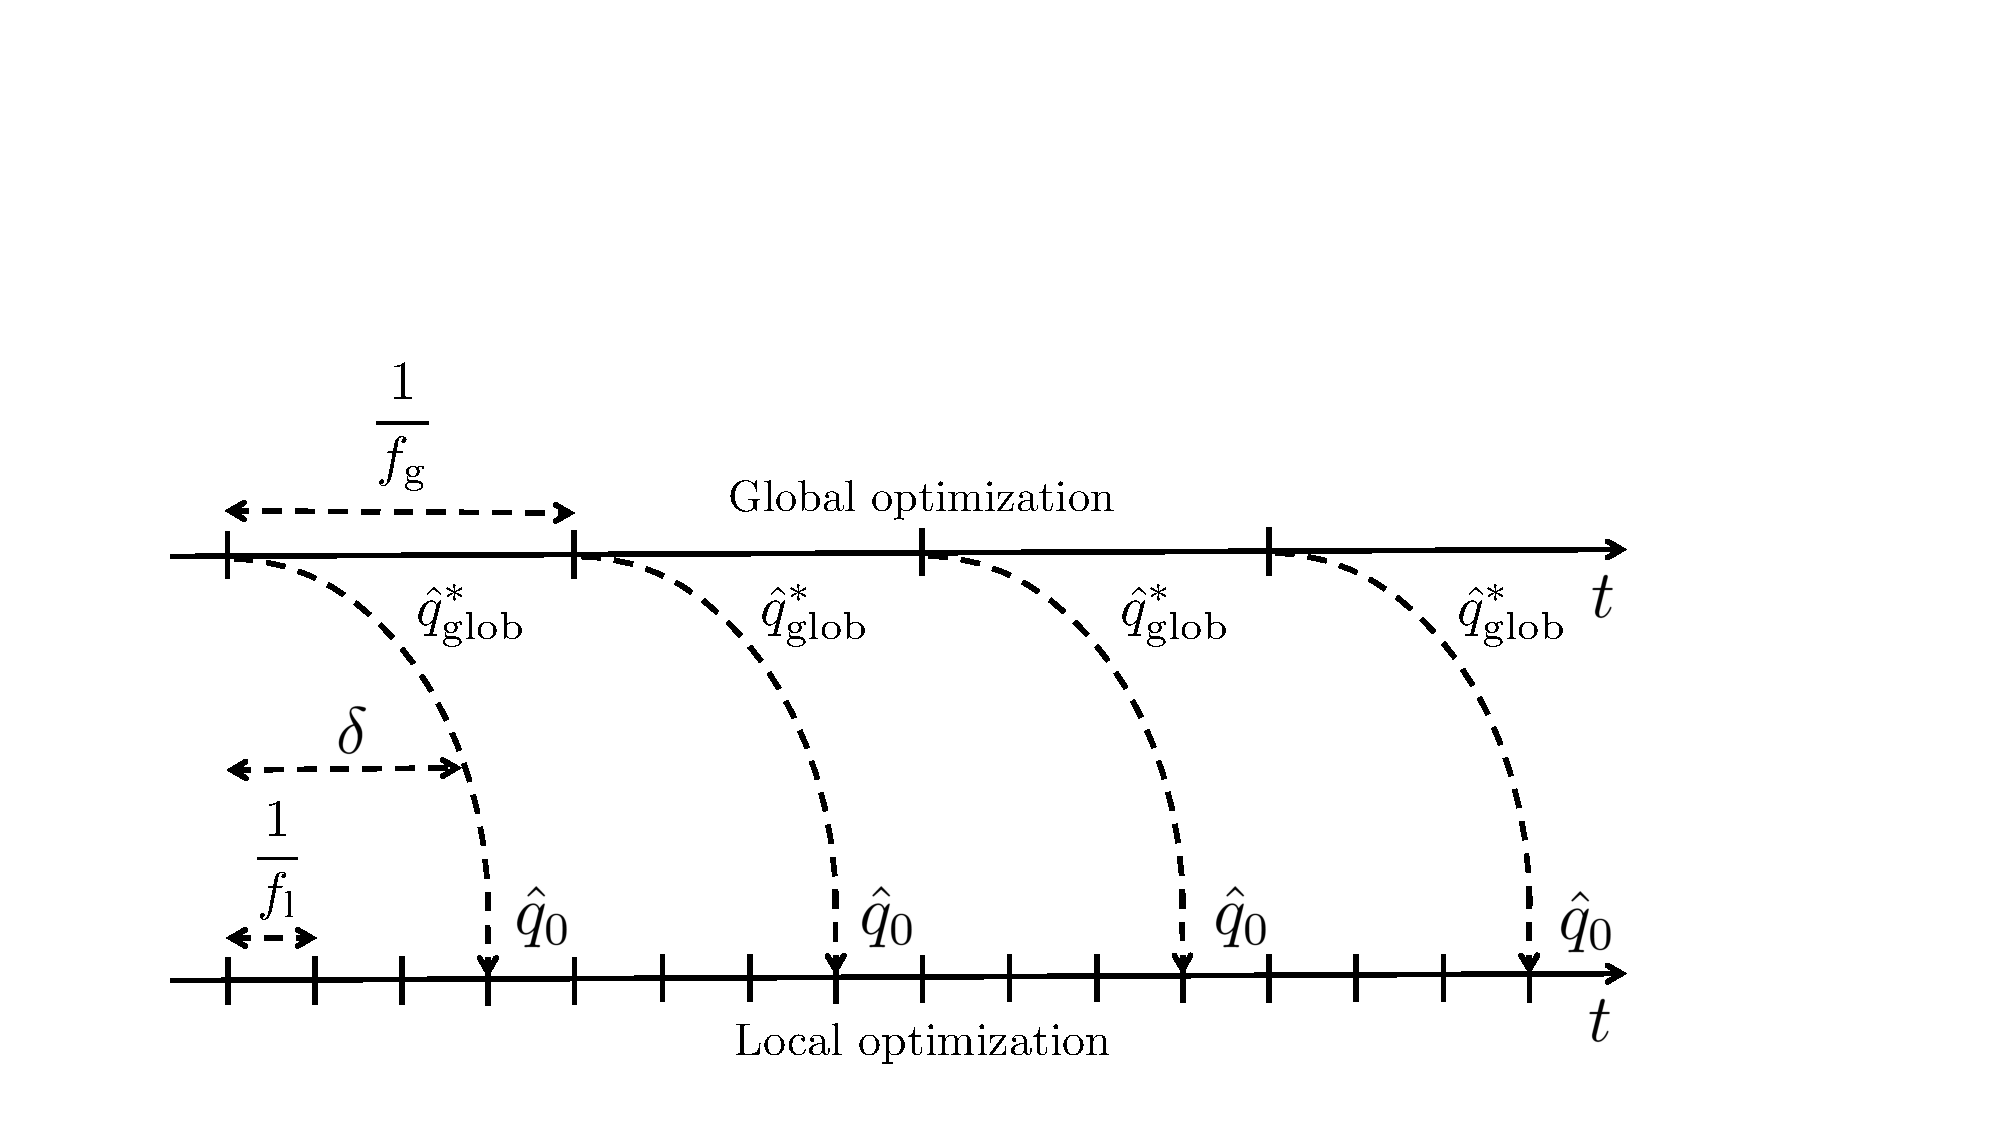
\includegraphics[width=1.0\columnwidth]{promasens/figures/methodology/optimization_scheduling_v2_cropped.pdf}\label{fig:promasens:optimization_scheduling}}\\
    % \subfigure[Local optimization: gradient descent]{\includegraphics[width=1.0\columnwidth]{promasens/figures/methodology/blockdiagram_gradient_descent_v4_cropped.pdf}\label{fig:promasens:blockdiagram_gradient_descent}}
    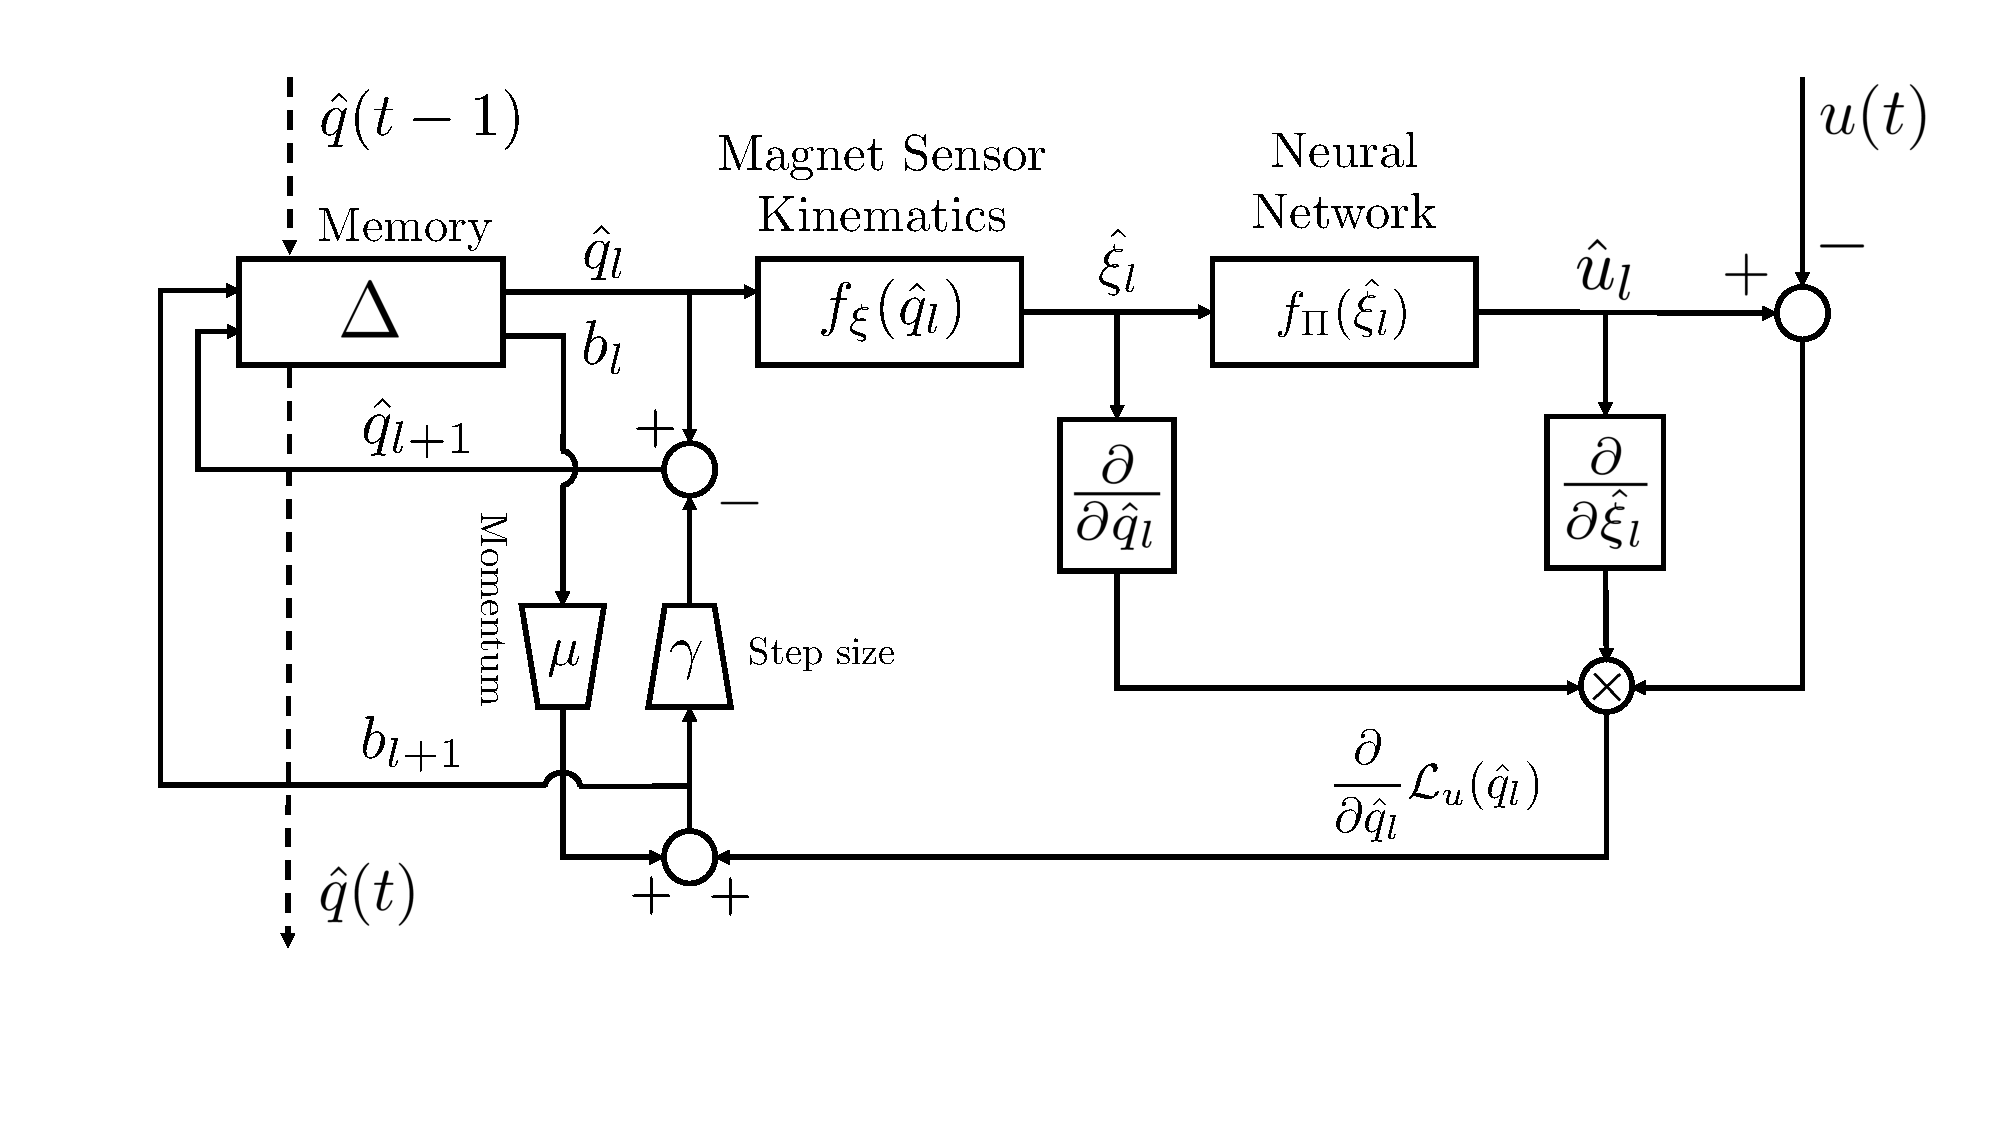
\includegraphics[width=1.0\columnwidth]{promasens/figures/methodology/blockdiagram_gradient_descent_v6_cropped.pdf}
    \caption{% In panel (a), we visualize the scheduling of our chosen optimization strategy: global optimization involving grid search is running at a frequency $f_\mathrm{g}$. In parallel, local gradient descent is performed at a frequency $f_\mathrm{l}$. The global optimization solution arrives $\hat{q}_\mathrm{glob}^*(t-\delta)$ at the local optimization with a delay of $\delta$ and is used to initialize $\hat{q}_0$ for the gradient descent. In all other instances, the gradient descent is initialized with the locally optimized solution $\hat{q}(t-1)$ from the previous time-step. 
    % Panel (b) 
    A block-diagram of the gradient descent as an iterative update loop for the configuration belief $\hat{q}(t)$. The gradient descent is initialized with the optimized solution $\hat{q}_0 = \hat{q}(t-1)$ from the previous time-step. Note that during the iterative loop, $\hat{q}_{l+1}$ updates $\hat{q}_{l}$ in the memory block.}\label{fig:promasens:blockdiagram_gradient_descent}
\end{figure}


\subsection{Data-driven sensor measurement model}
\label{sec:promasens:data_driven_approach}
We use a data-driven approach to learn the forward sensor model $\hat{u} = f_{\pi}(\xi_{j})$ for each sensor using a neural network parameterized with $\pi$.
We note that the same neural network weights can be shared for all sensors, but oftentimes performance can be improved by training a specialized model with weights $\pi_j$ for each sensor.
During training on a dataset of length $n_\mathrm{t}$, we minimize the Mean Squared Error (MSE) error between the predicted sensor measurement $\hat{u}_j$ and the actual sensor measurement $u_j$:
\begin{equation}\small
    \min_{\pi} \frac{1}{n_\mathrm{t}} \sum_{t = 0}^{n_\mathrm{t}} \left ( f_{\pi}(\xi_{j}(t)) - u_j(t) \right )^2,
\end{equation}
where $t$ denotes the current time index.
Note that whenever we omit the time index in our notation, we always refer to the current time $t$.
Finally, to simplify the notation, we combine each sensor measurement prediction $u_j \in \mathbb{R}$ into an array $u \in \mathbb{R}^{n_\mathrm{s}}$ and stack the neural networks as %$u = f_\pi(\xi)$
$f_\Pi(\xi): \xi \rightarrow u$. We discuss the choice of the specific network architecture later in Section~\ref{sec:promasens:pcc_simulations}.

\subsection{Proprioception by optimizing configuration estimate}
\label{sub:promasens:proprioception_optimization}

Now, that we are able to predict the sensor measurement $\hat{u}$ using the composition of the kinematics $f_\xi(\hat{q})$ and the neural networks $f_\Pi(\hat{\xi})$, we need to optimize the configuration estimate $\hat{q}$ for the predictions $\hat{u}$ to match the actual sensor measurements $u$ as closely as possible.
We capture the error between the predicted sensor measurements $\hat{u}$ and the actual sensor measurements $u$ by the MSE loss function we strive to minimize
\begin{equation}\small\label{eq:promasens:proprioception_loss}
    \mathcal{L}_{u}(\hat{q}) = \sum_{j=1}^{n_\mathrm{s}} \frac{\left ( f_\pi(\xi_j) - u_j \right )^2}{n_\mathrm{s}}
\end{equation}
Accordingly, the optimal configuration estimate $\hat{q}$ can be found with
\begin{equation}\small
    \hat{q} = \mathrm{argmin} \: \mathcal{L}_{u}(\hat{q}_l).
\end{equation}

% We employ a dual optimization strategy with global grid search and local gradient descent optimization running in parallel, as visualized in Fig.~\ref{fig:promasens:optimization_scheduling}. As the grid search is computationally expensive, we run it at a frequency of $f_\mathrm{g} \ll f_\mathrm{l}$, where $f_\mathrm{l}$ represents the sampling rate of the gradient descent.
% As we detail in Algorithm~\ref{alg:proprioception}, the gradient descent is nominally initialized with the best estimate of the previous time-step $\hat{q}_0 (t) = \hat{q}(t-1)$.
% When global optimization estimates are available, which are expected to arrive with a computational delay of $\delta$, we use those as an initial condition for the gradient descent.

We optimize the cost function \eqref{eq:promasens:proprioception_loss} through iterative gradient descent, as detailed in Fig.~\ref{fig:promasens:blockdiagram_gradient_descent}. The gradient descent is initialized with the best estimate of the previous time-step $\hat{q}_0 (t) = \hat{q}(t-1)$.
% For the gradient descent itself, detailed in Fig.\ref{fig:promasens:blockdiagram_gradient_descent}, we iteratively
As common in literature, we optimize the state belief $\hat{q}_l$ with a step size $\gamma$ and the momentum $\mu$ using the Jacobian of the loss $\frac{\partial}{\partial \hat{q}_t} \mathcal{L}_{u}(\hat{q})$
\begin{equation}\small\label{eq:promasens:gradient_descent}
    b_{l+1} = \mu \, b_l + \frac{\partial}{\partial \hat{q}_t} \mathcal{L}_{u}(\hat{q}), \quad \hat{q}_{l+1} = \hat{q}_l - \gamma \, b_{l+1}.
\end{equation}
We can use the chain rule to derive an analytical expression for the gradient of the loss incorporating the gradient of the magnet sensor kinematics $\partial_{\hat{q}} f_{\mathrm{\xi}}(\hat{q})$ and the gradient of the neural network $\partial_{\hat{\xi}} f_\Pi (\hat{\xi})$:
\begin{equation}\small
    \frac{\partial}{\partial \hat{q}} \mathcal{L}_{u}(\hat{q}) = \frac{2}{n_\mathrm{s}} \left ( \frac{\partial }{\partial {\hat{q}}} f_{\mathrm{\xi}}(\hat{q}) \right )^\mathrm{T} \, \left ( \frac{\partial}{\partial {\hat{\xi}}} f_\Pi(\hat{\xi}) \right )^\mathrm{T} \, (\hat{u} - u).
\end{equation}
After executing the gradient descent for $n_\mathrm{it}$ iterations, we evaluate which iteration $l^*$ had the lowest loss $\mathcal{L}_{u}$ and accordingly select $\hat{q}(t) = \hat{q}_{l^*}$ as the best configuration estimate of time-step $t$.

\section{Piecewise constant curvature simulations}\label{sec:promasens:pcc_simulations}
We evaluate the proposed methodology for estimating the \gls{PCC} kinematic configuration $q \in \mathbb{R}^{3n_\mathrm{b}}$ of soft continuum robots thoroughly in simulations.
The PCC model allows for bending and elongation of each segment in 3D space. Please refer to Appendix~\ref{sub:promasens:kinematic_model_pcc} for more details.
We vary the number of robot segments $n_\mathrm{b}$, remove and add sensors (i.e. change $n_\mathrm{s}$), modify the arrangement of sensors, and the direction of the earth's magnetic field $n_\mathrm{e}$. 
To motivate some of the unique advantages of our method, we use the same learned neural network weights for all these trials.

\begin{landscape}
\begingroup
\setlength{\tabcolsep}{2pt} % Default value: 6pt
\begin{table*}[hbt]
\centering
\caption{
Simulation results: First, we report the absolute Root Mean-Squared Error (RMSE) $e_{u}$ of sensor measurement predictions on the test set averaged across all sensors on the robot. Next, we state the relative RMSE [\%] of each robot configuration estimate. All results are trained on a trajectory with randomly sampled configurations and sensor kinematic parameters for each segment separately and evaluated on a lemniscate trajectory.
The first section applies our methodology to robots consisting of a different number of segments $n_\mathrm{b}$ with three sensors attached to the tip of each segment.
The number of sensors is varied in the second section for a three-segment robot with all sensors placed symmetrically. 
The third set of trials then investigates how robust the method is to change the kinematic parameters of the sensors, such as the tilting angle of the sensors $\psi_\mathrm{s}$ and the radial distance of the sensors $d_{\mathrm{s},\mathrm{r}}$.
Finally, we apply the earth's magnetic field along different cardinal directions in the inertial frame.
The RMSE of the configuration estimates is normalized with the range of the dataset for each configuration variable as stated in \eqref{eq:promasens:relative_RMSE}. We report the error as $\text{mean} \pm \text{stdev}$ and compute the statistics over three different random seeds. The random seed determines at the start of the training the initialization of the neural network weights.
}
% \begin{tabular}{l r rrr rrr rrr}\toprule
% \textbf{Simulation} & $e_{u}$ [mT] & $e_{\Delta_{x,1}}$ [\%] & $e_{\Delta_{y,1}}$ [\%] & $e_{\delta L_1}$ [\%] & $e_{\Delta_{x,2}}$ [\%] & $e_{\Delta_{y,2}}$ [\%] & $e_{\delta L_2}$ [\%] & $e_{\Delta_{x,3}}$ [\%] & $e_{\Delta_{y,3}}$ [\%] & $e_{\delta L_3}$ [\%]\\
% \midrule
% \# of segments: $n_\mathrm{b} = 1$ & $1.5 \pm 0.2$ & $1.7 \pm 1.0$ & $1.8 \pm 1.1$ & $2.8 \pm 0.6$ & - & - & - & - & - & -\\
% \# of segments: $n_\mathrm{b} = 2$ & $1.5 \pm 0.1$ & $4.2 \pm 1.3$ & $3.9 \pm 0.6$ & $6.3 \pm 1.3$ & $2.3 \pm 0.6$ & $2.2 \pm 0.3$ & $4.1 \pm 1.3$ & - & - & -\\
% \# of segments: $n_\mathrm{b} = 3$ & $1.5 \pm 0.2$ & $3.7 \pm 2.1$ & $4.7 \pm 1.6$ & $6.0 \pm 2.0$ & $2.6 \pm 1.6$ & $2.5 \pm 1.5$ & $5.5 \pm 1.6$ & $1.6 \pm 1.2$ & $1.6 \pm 1.1$ & $2.7 \pm 1.4$\\
% \midrule
% \# of sensors: $n_\mathrm{s} = 6$ & $1.5 \pm 0.2$ & $3.9 \pm 1.2$ & $24.4 \pm 2.7$ & $8.4 \pm 2.6$ & $2.5 \pm 1.3$ & $53.2 \pm 5.0$ & $6.0 \pm 1.7$ & $1.5 \pm 1.1$ & $52.3 \pm 7.3$ & $3.1 \pm 1.0$\\
% \# of sensors: $n_\mathrm{s} = 9$ & $1.5 \pm 0.2$ & $3.7 \pm 2.1$ & $4.7 \pm 1.6$ & $6.0 \pm 2.0$ & $2.6 \pm 1.6$ & $2.5 \pm 1.5$ & $5.5 \pm 1.6$ & $1.6 \pm 1.2$ & $1.6 \pm 1.1$ & $2.7 \pm 1.4$\\
% \# of sensors: $n_\mathrm{s} = 12$ & $1.5 \pm 0.1$ & $3.7 \pm 1.6$ & $3.9 \pm 1.3$ & $4.6 \pm 2.4$ & $2.6 \pm 1.3$ & $2.6 \pm 1.2$ & $4.4 \pm 1.9$ & $1.6 \pm 1.2$ & $1.5 \pm 1.3$ & $2.5 \pm 1.6$\\
% \# of sensors: $n_\mathrm{s} = 18$ & $1.6 \pm 0.2$ & $3.2 \pm 1.5$ & $3.5 \pm 1.3$ & $4.2 \pm 1.8$ & $2.4 \pm 1.3$ & $2.5 \pm 1.2$ & $4.4 \pm 1.8$ & $1.5 \pm 1.3$ & $1.3 \pm 1.1$ & $2.5 \pm 1.5$\\
% \midrule
% nominal & $1.5 \pm 0.2$ & $3.7 \pm 2.1$ & $4.7 \pm 1.6$ & $6.0 \pm 2.0$ & $2.6 \pm 1.6$ & $2.5 \pm 1.5$ & $5.5 \pm 1.6$ & $1.6 \pm 1.2$ & $1.6 \pm 1.1$ & $2.7 \pm 1.4$\\
% sensors tilted: $\psi_\mathrm{s} = \SI{10}{\degree}$ & $1.5 \pm 0.2$ & $8.1 \pm 4.0$ & $6.4 \pm 2.0$ & $4.7 \pm 0.7$ & $5.1 \pm 2.3$ & $3.8 \pm 0.8$ & $5.6 \pm 2.4$ & $2.8 \pm 1.2$ & $1.9 \pm 0.8$ & $4.1 \pm 0.6$\\
% $d_{\mathrm{s},\mathrm{r}} = \SI{16}{mm}, \psi_\mathrm{s} = \SI{10}{\degree}$ & $1.5 \pm 0.1$ & $4.0 \pm 2.1$ & $4.3 \pm 1.6$ & $4.6 \pm 1.3$ & $2.9 \pm 0.3$ & $2.4 \pm 0.3$ & $5.2 \pm 1.6$ & $1.6 \pm 1.0$ & $1.6 \pm 0.8$ & $3.1 \pm 1.0$ \\
% % \midrule
% % FEM nominal & $0.0 \pm 0.0$ & $0.0 \pm 0.0$ & $0.0 \pm 0.0$ & $0.0 \pm 0.0$ & $0.0 \pm 0.0$ & $0.0 \pm 0.0$ & $0.0 \pm 0.0$ & $0.0 \pm 0.0$ & $0.0 \pm 0.0$ & $0.0 \pm 0.0$\\
% \bottomrule
% \end{tabular}

\begin{tabular}{cl r rrr rrr rrr}\toprule
\textbf{Simulation} & \textbf{Specifications} & $e_{u}$ [mT] & $e_{\Delta_{x,1}}$ [\%] & $e_{\Delta_{y,1}}$ [\%] & $e_{\delta L_1}$ [\%] & $e_{\Delta_{x,2}}$ [\%] & $e_{\Delta_{y,2}}$ [\%] & $e_{\delta L_2}$ [\%] & $e_{\Delta_{x,3}}$ [\%] & $e_{\Delta_{y,3}}$ [\%] & $e_{\delta L_3}$ [\%]\\
\midrule
\multirow{3}{*}{\makecell{Variation of\\ \# of segments}} & $n_\mathrm{b}$=1, $n_\mathrm{s}$=3 & $0.015 \pm 0.002$ & $1.7 \pm 1.0$ & $1.8 \pm 1.1$ & $2.8 \pm 0.6$ & - & - & - & - & - & -\\
& $n_\mathrm{b}$=2, $n_\mathrm{s}$=6 & $0.015 \pm 0.001$ & $4.2 \pm 1.3$ & $3.9 \pm 0.6$ & $6.3 \pm 1.3$ & $2.3 \pm 0.6$ & $2.2 \pm 0.3$ & $4.1 \pm 1.3$ & - & - & -\\
& $n_\mathrm{b}$=3, $n_\mathrm{s}$=9 & $0.015 \pm 0.002$ & $3.7 \pm 2.1$ & $4.7 \pm 1.6$ & $6.0 \pm 2.0$ & $2.6 \pm 1.6$ & $2.5 \pm 1.5$ & $5.5 \pm 1.6$ & $1.6 \pm 1.2$ & $1.6 \pm 1.1$ & $2.7 \pm 1.4$\\
\midrule
\multirow{4}{*}{\makecell{Variation of\\ \# of sensors}} &$n_\mathrm{b}$=3, $n_\mathrm{s}$=6 & $0.015 \pm 0.002$ & $3.9 \pm 1.2$ & $24.4 \pm 2.7$ & $8.4 \pm 2.6$ & $2.5 \pm 1.3$ & $53.2 \pm 5.0$ & $6.0 \pm 1.7$ & $1.5 \pm 1.1$ & $52.3 \pm 7.3$ & $3.1 \pm 1.0$\\
&$n_\mathrm{b}$=3, $n_\mathrm{s}$=9 & $0.015 \pm 0.002$ & $3.7 \pm 2.1$ & $4.7 \pm 1.6$ & $6.0 \pm 2.0$ & $2.6 \pm 1.6$ & $2.5 \pm 1.5$ & $5.5 \pm 1.6$ & $1.6 \pm 1.2$ & $1.6 \pm 1.1$ & $2.7 \pm 1.4$\\
&$n_\mathrm{b}$=3, $n_\mathrm{s}$=12 & $0.015 \pm 0.001$ & $3.7 \pm 1.6$ & $3.9 \pm 1.3$ & $4.6 \pm 2.4$ & $2.6 \pm 1.3$ & $2.6 \pm 1.2$ & $4.4 \pm 1.9$ & $1.6 \pm 1.2$ & $1.5 \pm 1.3$ & $2.5 \pm 1.6$\\
&$n_\mathrm{b}$=3, $n_\mathrm{s}$=18 & $0.016 \pm 0.002$ & $3.2 \pm 1.5$ & $3.5 \pm 1.3$ & $4.2 \pm 1.8$ & $2.4 \pm 1.3$ & $2.5 \pm 1.2$ & $4.4 \pm 1.8$ & $1.5 \pm 1.3$ & $1.3 \pm 1.1$ & $2.5 \pm 1.5$\\
\midrule
Nominal & $n_\mathrm{b}$=3, $n_\mathrm{s}$= 9 & $0.015 \pm 0.002$ & $3.7 \pm 2.1$ & $4.7 \pm 1.6$ & $6.0 \pm 2.0$ & $2.6 \pm 1.6$ & $2.5 \pm 1.5$ & $5.5 \pm 1.6$ & $1.6 \pm 1.2$ & $1.6 \pm 1.1$ & $2.7 \pm 1.4$\\
Sensors tilted & $\psi_\mathrm{s}$=\SI{10}{\degree} & $0.015 \pm 0.002$ & $8.1 \pm 4.0$ & $6.4 \pm 2.0$ & $4.7 \pm 0.7$ & $5.1 \pm 2.3$ & $3.8 \pm 0.8$ & $5.6 \pm 2.4$ & $2.8 \pm 1.2$ & $1.9 \pm 0.8$ & $4.1 \pm 0.6$\\
Sensors shifted & $d_{\mathrm{s},\mathrm{r}}$=\SI{16}{mm} & $0.017 \pm 0.003$ & $3.4 \pm 1.5$ & $4.0 \pm 1.3$ & $6.2 \pm 2.5$ & $2.6 \pm 1.0$ & $2.8 \pm 1.8$ & $6.7 \pm 0.9$ & $1.6 \pm 1.2$ & $1.6 \pm 1.0$ & $4.0 \pm 2.0$ \\
\midrule
\multirow{3}{*}{\makecell{Earth\\ magnetic\\ field}} & $n_\mathrm{e}$=$(1,0,0)$ & $0.012 \pm 0.002$ & $2.0 \pm 0.4$ & $2.4 \pm 1.1$ & $4.3 \pm 1.3$ & $1.8 \pm 0.7$ & $1.9 \pm 0.3$ & $3.6 \pm 2.0$ & $1.5 \pm 0.3$ & $1.6 \pm 0.4$ & $3.2 \pm 0.9$\\
& $n_\mathrm{e}$=$(0,1,0)$ & $0.012 \pm 0.002$ & $1.9 \pm 0.5$ & $2.5 \pm 0.8$ & $3.8 \pm 1.1$ & $1.9 \pm 0.5$ & $2.0 \pm 0.2$ & $3.4 \pm 1.6$ & $1.5 \pm 0.3$ & $1.6 \pm 0.4$ & $3.3 \pm 0.8$\\
& $n_\mathrm{e}$=$(0,0,1)$ & $0.012 \pm 0.001$ & $2.0 \pm 0.7$ & $2.6 \pm 0.9$ & $4.1 \pm 0.9$ & $1.6 \pm 0.3$ & $1.7 \pm 0.3$ & $4.9 \pm 1.5$ & $1.5 \pm 0.5$ & $1.4 \pm 0.1$ & $3.9 \pm 0.3$\\
% \midrule
% FEM nominal & $0.0 \pm 0.0$ & $0.0 \pm 0.0$ & $0.0 \pm 0.0$ & $0.0 \pm 0.0$ & $0.0 \pm 0.0$ & $0.0 \pm 0.0$ & $0.0 \pm 0.0$ & $0.0 \pm 0.0$ & $0.0 \pm 0.0$ & $0.0 \pm 0.0$\\
\bottomrule
\end{tabular}
\label{tab:results_pcc_simulations}
\end{table*}
\endgroup
\end{landscape}

\begin{figure*}[hbt]
\centering
    \subfigure[Magnetic field for a three-segment robot]{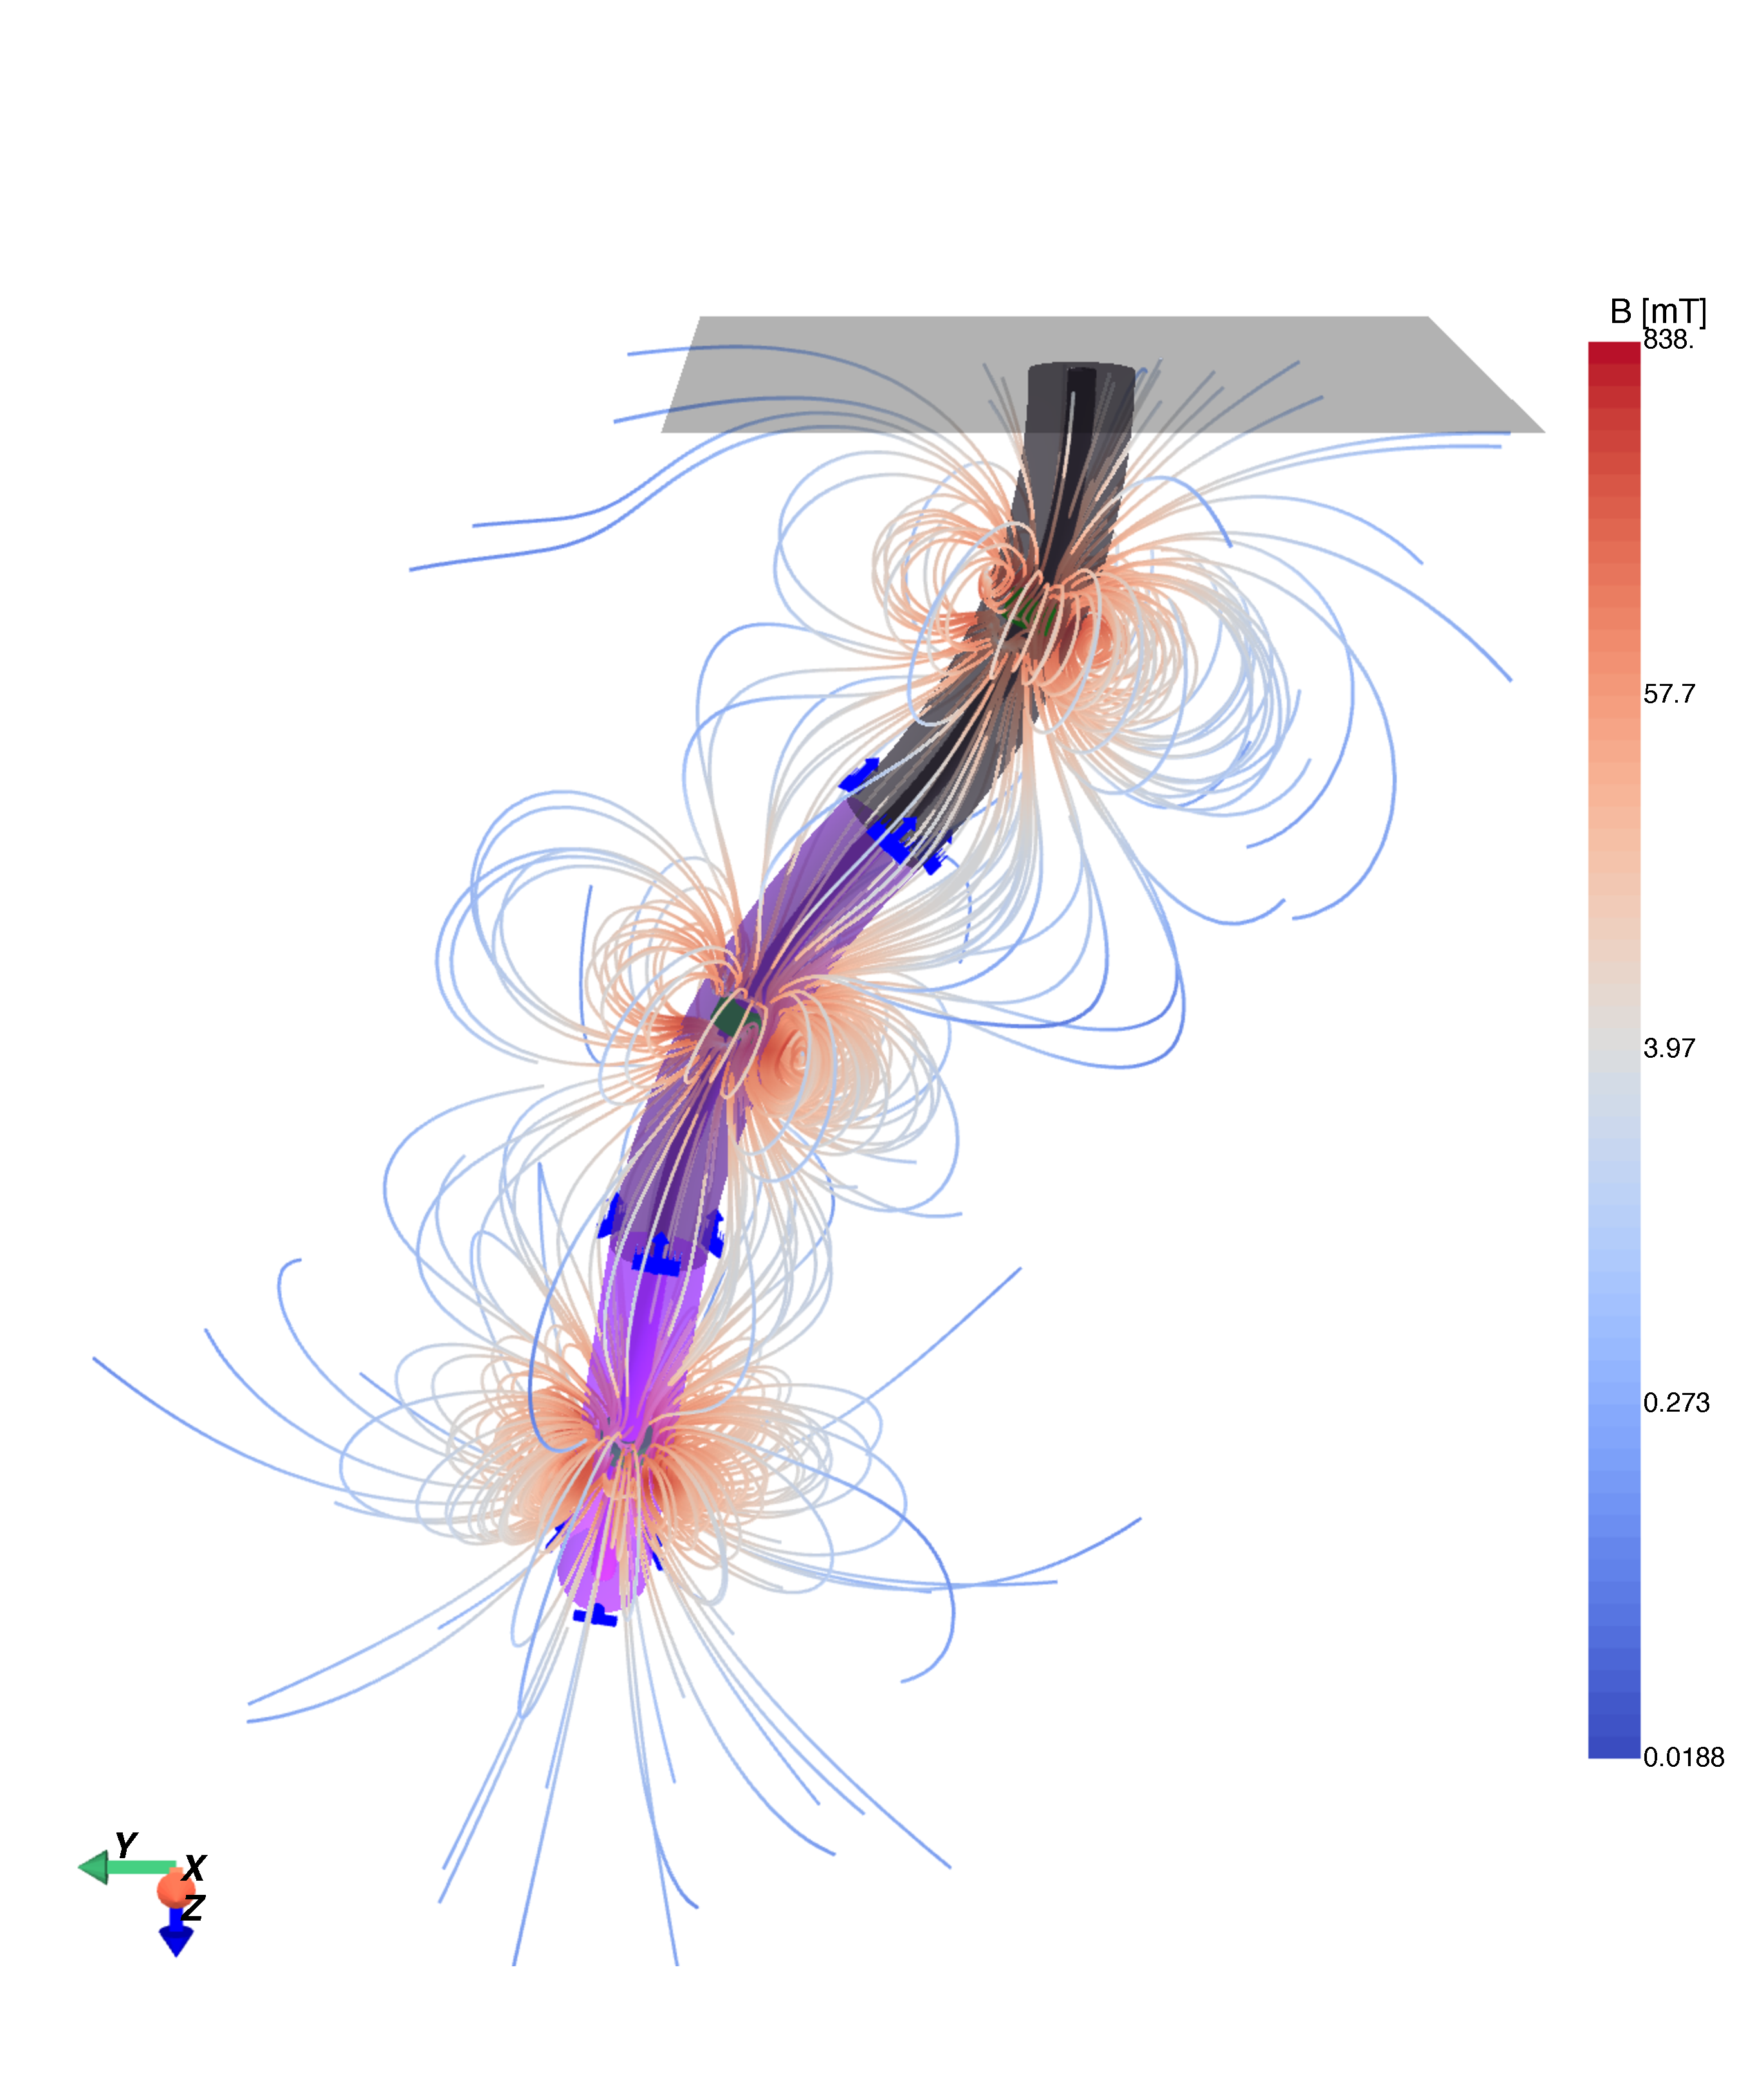
\includegraphics[width=0.3\textwidth]{promasens/figures/simulation_setup/analytical_simulation_three_segment_v2_cropped.pdf}}
    \subfigure[Simulated sensor failure]{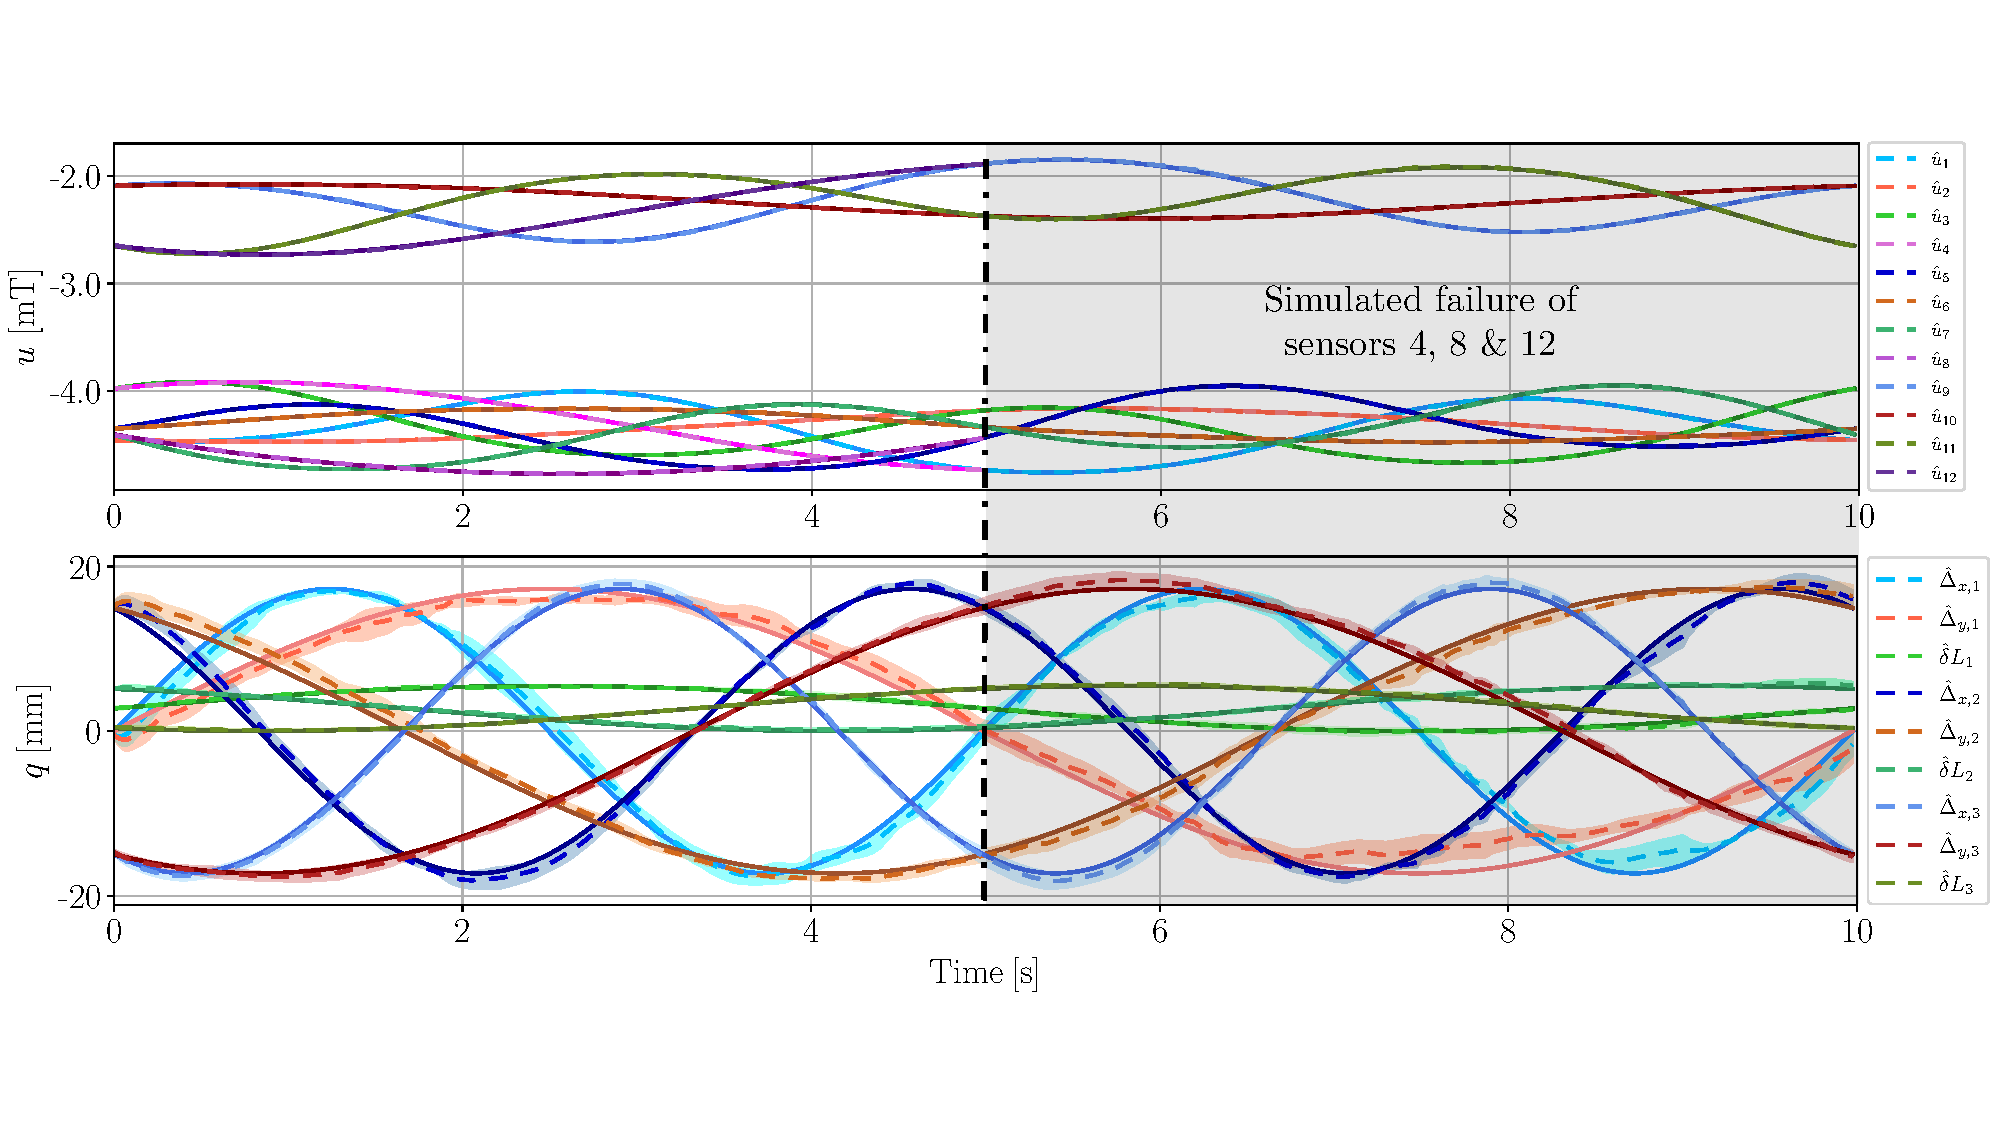
\includegraphics[width=0.68\textwidth]{promasens/figures/simulation_results/pcc/simulated_sensor_failure_cropped.pdf}\label{fig:promasens:simulated_sensor_failure}}
\caption{\textbf{Panel (a):} Simulated magnetic field of a robot with three segments. The blue arrows mark the measurement directions of the sensors, the magnets are rendered in green and the three segments are visualized in a color sequence from black to violet. The magnetic flux density $B$ is shown via streamlines and logarithmic coloring. \textbf{Panel (b)}: Sensor measurement predictions (top) and configuration estimates (bottom) for a three-segment robot with twelve sensors nominally. We simulate a sensor failure of the 4th, 8th, and 12th sensors after \SI{5}{s} of trajectory time by removing the measurements of these sensors from the gradient descent. This can be compensated automatically by the redundancy of the sensor configuration. We plot the ground-truth values $u$ and $q$ in solid, the estimate $\hat{u}$ and $\hat{q}$ as a mean over three random seeds with dashed lines and the standard deviation as an error band.}
\end{figure*}

\subsection{Simulation setup}\label{sub:promasens:pcc_simulations:simulation_setup}
In our simulations, we consider a robot consisting of one, two, or three segments. % which all behave according to the Constant Curvature (CC) assumption and can also elongate~\cite{della2020improved}. 
All cylindrical segments have an unextended length of $L_{0,i} = \SI{110}{mm}$ and a radius of $d_i = \SI{22}{mm}$. Each segment has a neodymium N50 ring magnet of outer diameter \SI{12}{mm}, inner diameter \SI{6}{mm} and thickness \SI{6}{mm} integrated along the backbone at a distance of $d_{\mathrm{m}_k} = \SI{55}{mm}$ from the base of the segment.
In the nominal case, three sensors are placed symmetrically in the tip plane of each segment at a radius of \SI{13}{mm} from the center with the sensor measurement direction pointing along the local, negative z-axis of the tip plane $\{S_i\}$. We also consider alternative placements of the sensors, which we further detail in Section~\ref{sub:promasens:simulation_pcc_results}.

% \subsection{Magnetic field simulation}
% The crucial component of our simulation is the prediction of the magnetic field and corresponding sensor measurements for a given pose of the magnets.
% For this, we leverage Magpylib~\cite{magpylib2020}, a Python package for computing 3D static magnetic fields using analytical solutions.
We build on Magpylib~\cite{magpylib2020} to simulate the magnetic field behavior.
We model the magnets as cylindrical neodymium grade N50 rings with a magnetization of \SI{1450}{mT} in the local z-direction. 
After simulating the magnetic field, we rotate the B-field into the local reference frame of each sensor and take the local z-component of the magnetic flux density as the sensor measurement.
%Additionally, we add a static B-field representing the earth's magnetic field influence along the inertial x-axis and a magnitude of \SI{65}{\micro T}. To simulate the sensor measurements, we take into account the component of the B-field pointing along the local z-axis of the sensor.

% \subsection{Magnetic field simulation \textcolor{orange}{FEM}}
% We build on Netgen / NGSolve~\cite{netgen_ngsolve} to simulate the magnetic field behavior using \gls{FEM} by implementing the magnetostatic Maxwell equations.
% We model a cylindrical Neodymium grade N50 ring magnet with a magnetization of $M=(0,0,\SI{1.45}{T})^\mathrm{T}$ in local z-direction and a relative permeability of $\mu_r = 1.05$. 
% % Additionally, we add a static B-field representing the earth's magnetic field influence along the inertial x-axis and a magnitude of \SI{65}{\micro T}. To simulate the sensor measurements, we take into account the component of the B-field pointing along the local z-axis of the sensor.
% The remaining part of the control volume
% We mesh the magnets and the air with a maximum mesh size of \SI{6}{mm} and \SI{220}{mm} respectively.
% After solving the finite element problem, we rotate the B-field into the local reference frame for each sensor and take the z-component of the magnetic flux density as the sensor measurement.
%

\subsection{Prediction network}\label{sub:promasens:pcc_simulations:neural_network}
The training set consists of \SI{120000}{} random configurations sampled from uniform distribution $\Delta_{x,i} \sim \mathcal{U}(-\SI{20.7}{mm}, \SI{20.7}{mm})$, $\Delta_{y,i} \sim \mathcal{U}(-\SI{20.7}{mm}, \SI{20.7}{mm})$, and $\delta L_i \sim \mathcal{U}(0, \SI{5.5}{mm})$, where the upper bound represents a bending of the tip of \SI{54}{\degree} with respect to the base of a segment and an elongation of \SI{5}{\percent}. We also randomize the placement of the sensors in the training set. While in the nominal case, the first of the symmetrically placed sensors is placed on the local x-axis, we randomly sample an offset angle $\varphi_\mathrm{off} \sim \mathcal{U}(0, \frac{2\pi}{n_{\mathrm{s}_i}})$ for each training sample, where $n_{\mathrm{s}_i} = 3$ is the number of sensors per segment.
Finally, we also randomly sample the radial displacement of the sensors from the center with $d_{\mathrm{s}, \mathrm{r}} \sim \mathcal{U}(8.7, 17.3) \mathrm{mm}$ and consider a tilting of the sensors (e.g. a rotation around the tangential axis) with $\psi_\mathrm{s} \sim \mathcal{U}(\SI{-20}{\degree}, \SI{20}{\degree})$.
Before training, we randomly split off \SI{30}{\percent} of the training set for validation purposes.

We conducted a selection study involving hyperparameters and feed-forward neural network architectures (number of layers, nodes, and nonlinear activation layer types) on the validation set. % to select our training procedure for the sensor measurement prediction network. 
In particular, we aimed to generate a smooth loss landscape to improve the gradient descent convergence leading us to employ a Stochastic Gradient Descent (SGD) % ~\cite{ruder2016overview} 
optimizer in conjunction with the Stochastic Weight Averaging (SWA)~\cite{izmailov2018averaging} strategy.
The neural network itself %as depicted in Figure~\ref{fig:promasens:NNgradientdescent}
has $18$ layers in total and contains, after an initial 1D batch norm layer, four blocks and is concluded with a fully-connected layer at the end. Each block consists of a dropout with a probability of \SI{1}{\percent}, a linear layer, a ReLU, and a 1D batch norm layer. The hidden state is first increased to $96$ nodes, then to $256$ nodes, and finally reduced again to $64$ and $24$ nodes.
We minimize a Mean Squared Error (MSE) loss of the neural network prediction $\hat{u}_j(t)$ for $250$ epochs with batch size $650$ while setting an initial learning rate of $0.18$ for the cosine annealing learning rate scheduler~\cite{loshchilov2016sgdr}. The SWA~\cite{izmailov2018averaging} strategy is started after $125$ epochs.
% We train a neural network $f_{\pi_i}(\xi_j)$ for all sensors in each segment $i$.
We train the neural network such that all sensors in the $i^\mathrm{th}$ segment share the same weights $\pi_i$.
% The reason for this is that the sensors in the distal segment measure much lower magnetic field magnitudes than the sensors in the other segments as they are only influenced by one magnet (e.g. the magnet in the distal segment) resulting in poor convergence behavior when trained jointly on all segments.
When the training is finished, we select the model from the epoch with the lowest validation loss and save it for later testing.

\begin{figure*}[hbt]
  \centering
  \subfigure[$t=\SI{0}{s}$]{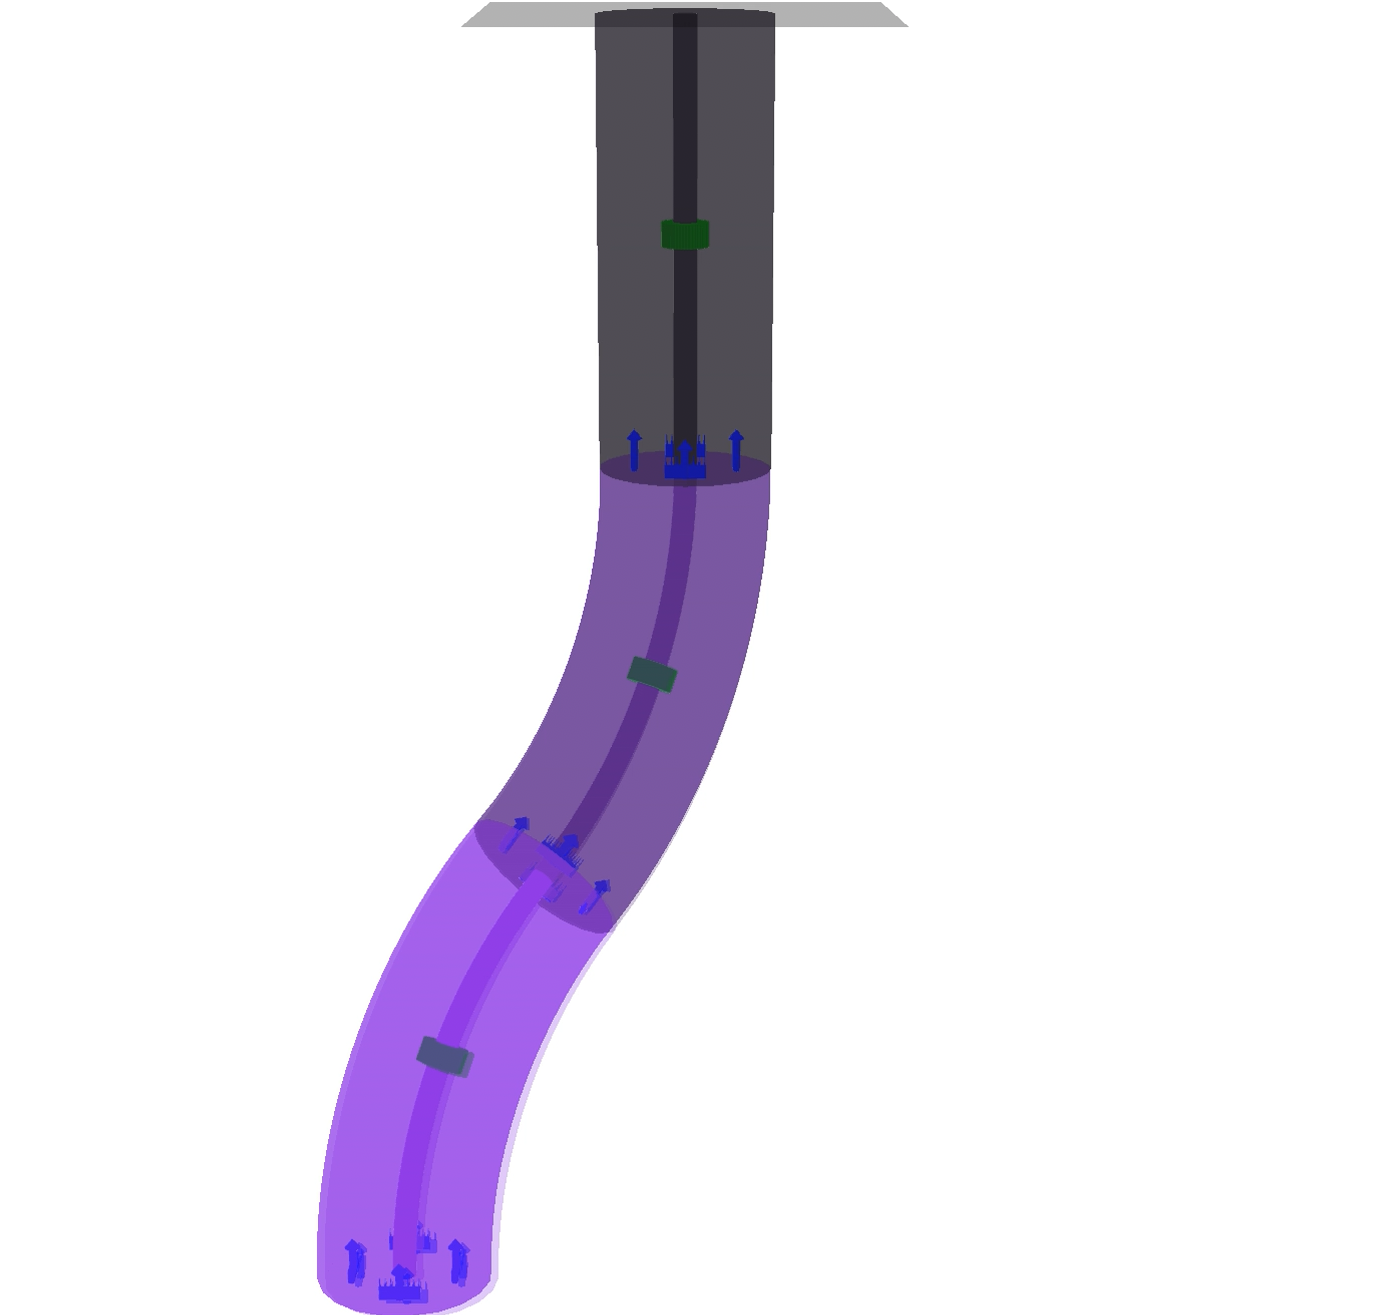
\includegraphics[width=0.161\textwidth]{promasens/figures/simulation_sequences/pcc_simulated_sensor_failure/simulated_sensor_failure_t=0s_cropped.png}}
  \hfill
  \subfigure[$t=\SI{2}{s}$]{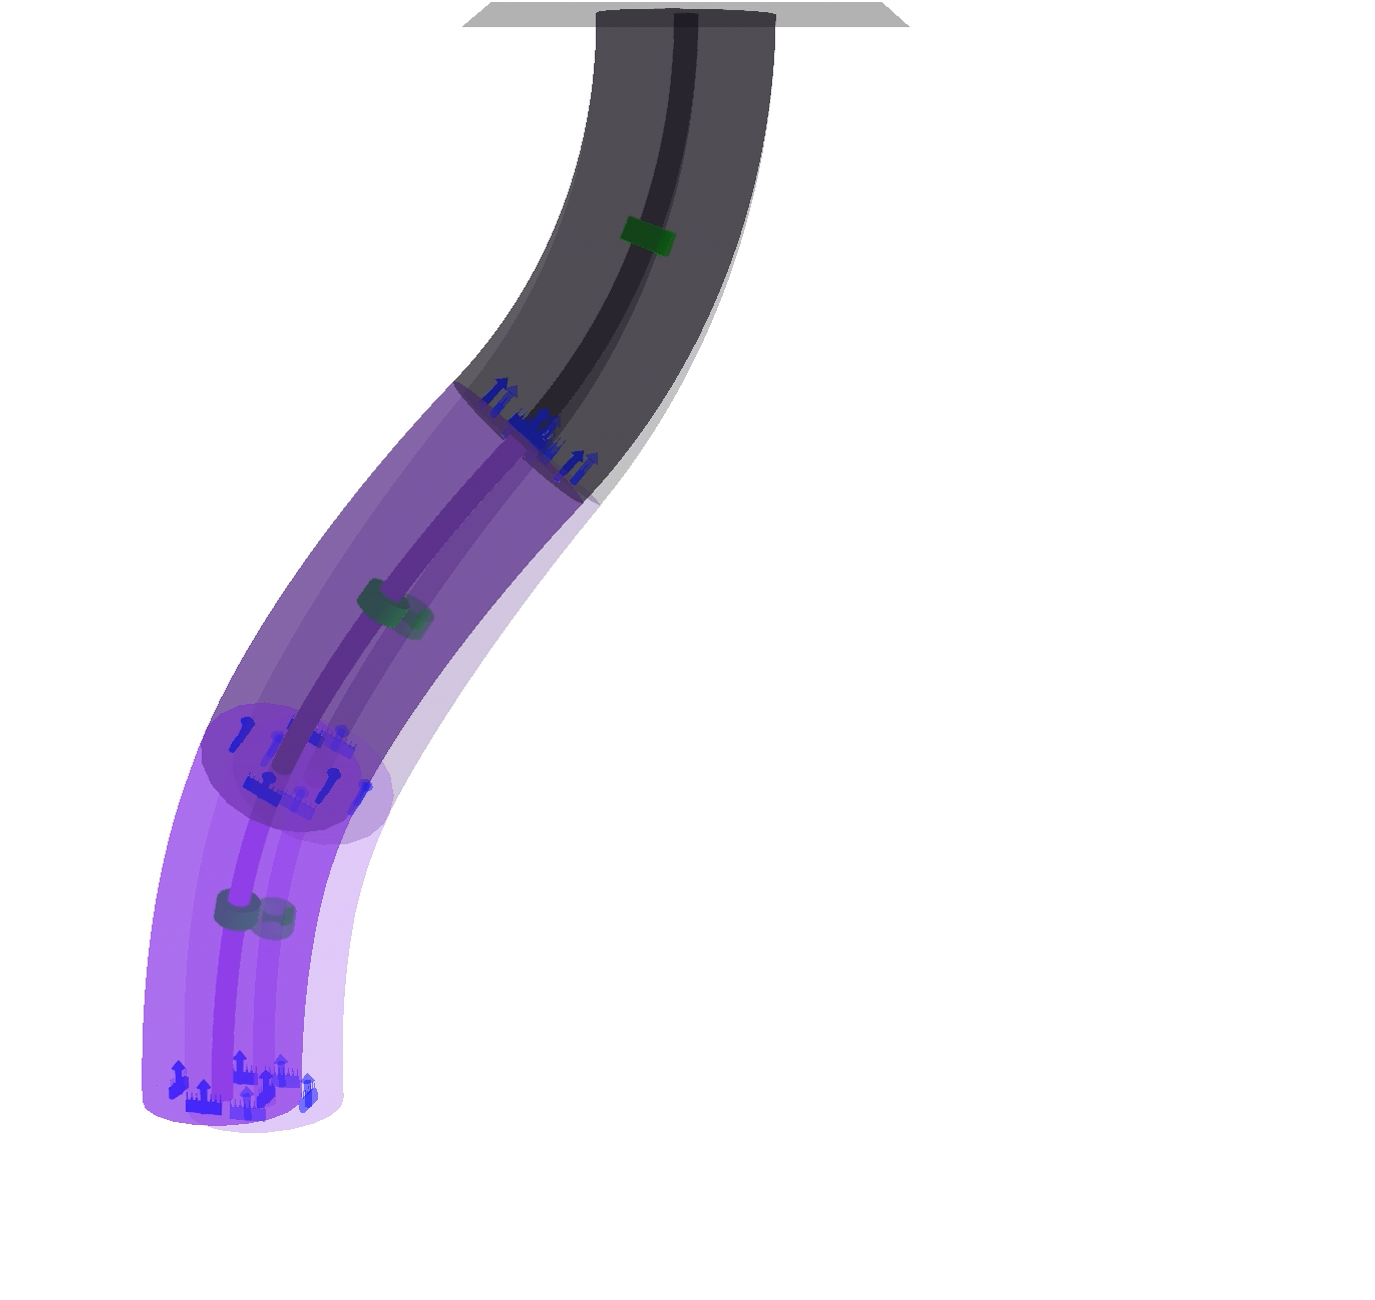
\includegraphics[width=0.161\textwidth]{promasens/figures/simulation_sequences/pcc_simulated_sensor_failure/simulated_sensor_failure_t=2s_cropped.png}}
  \hfill
  \subfigure[$t=\SI{4}{s}$]{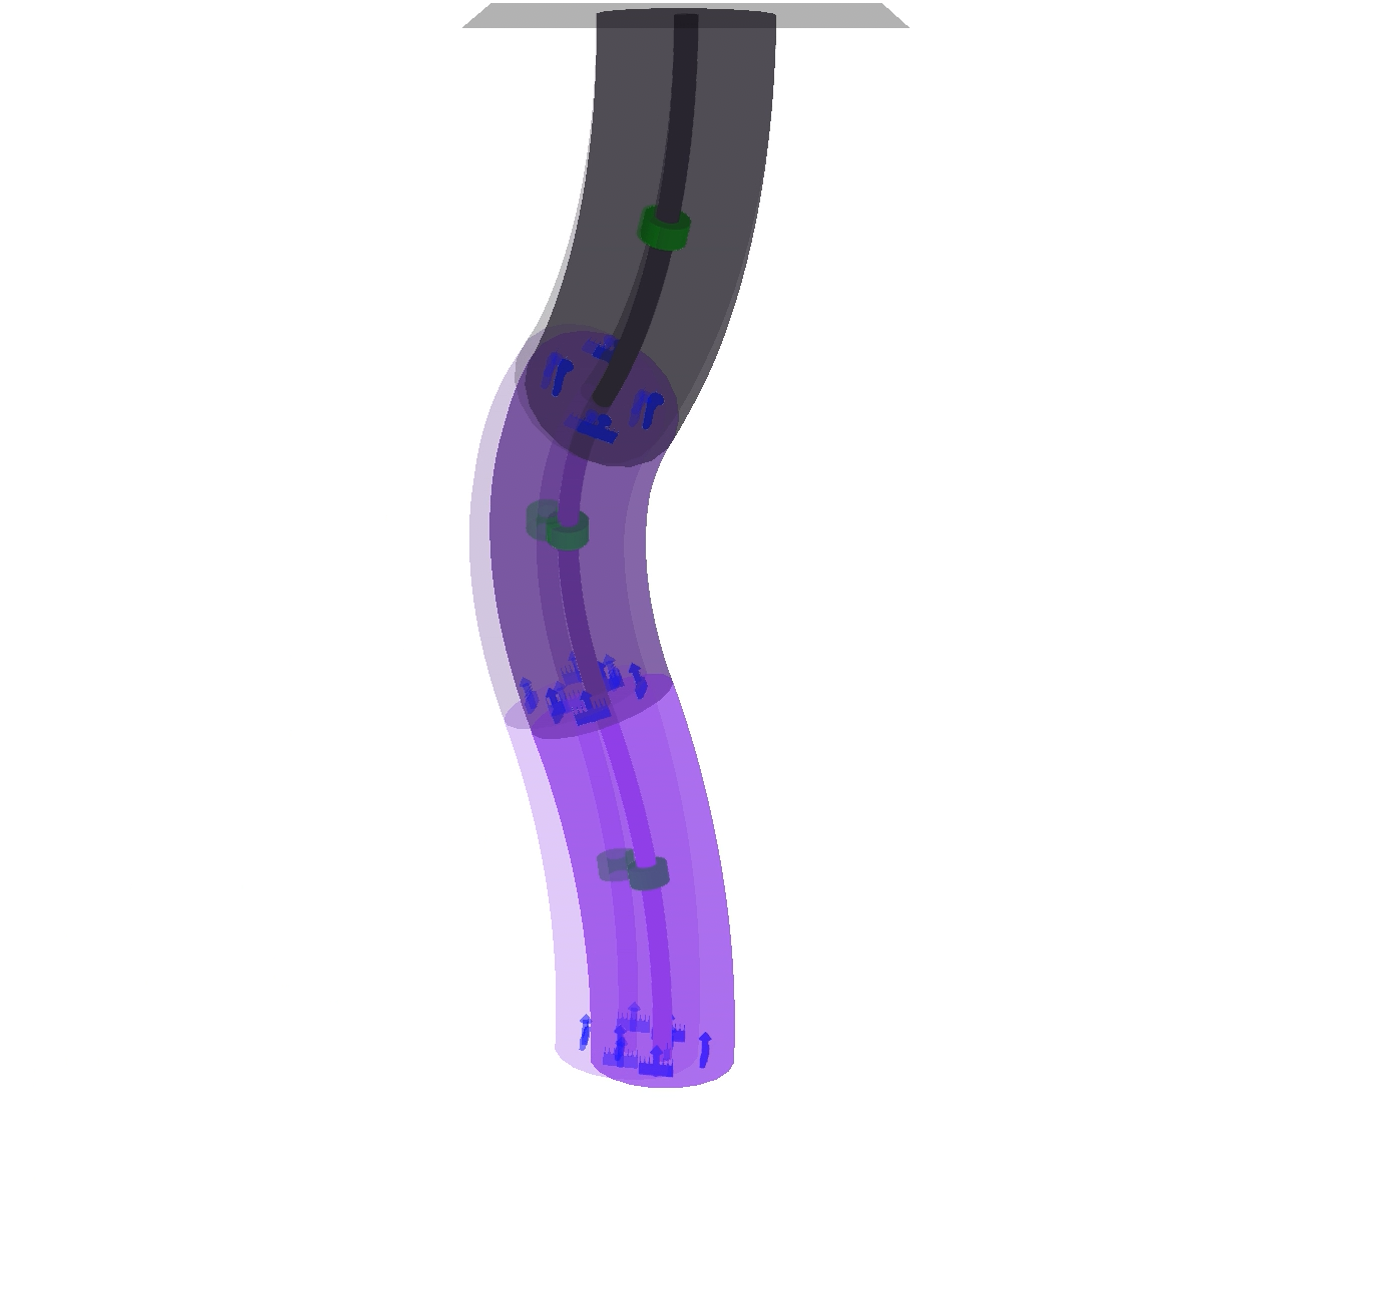
\includegraphics[width=0.161\textwidth]{promasens/figures/simulation_sequences/pcc_simulated_sensor_failure/simulated_sensor_failure_t=4s_cropped.png}}
  \hfill
  \subfigure[$t=\SI{6}{s}$]{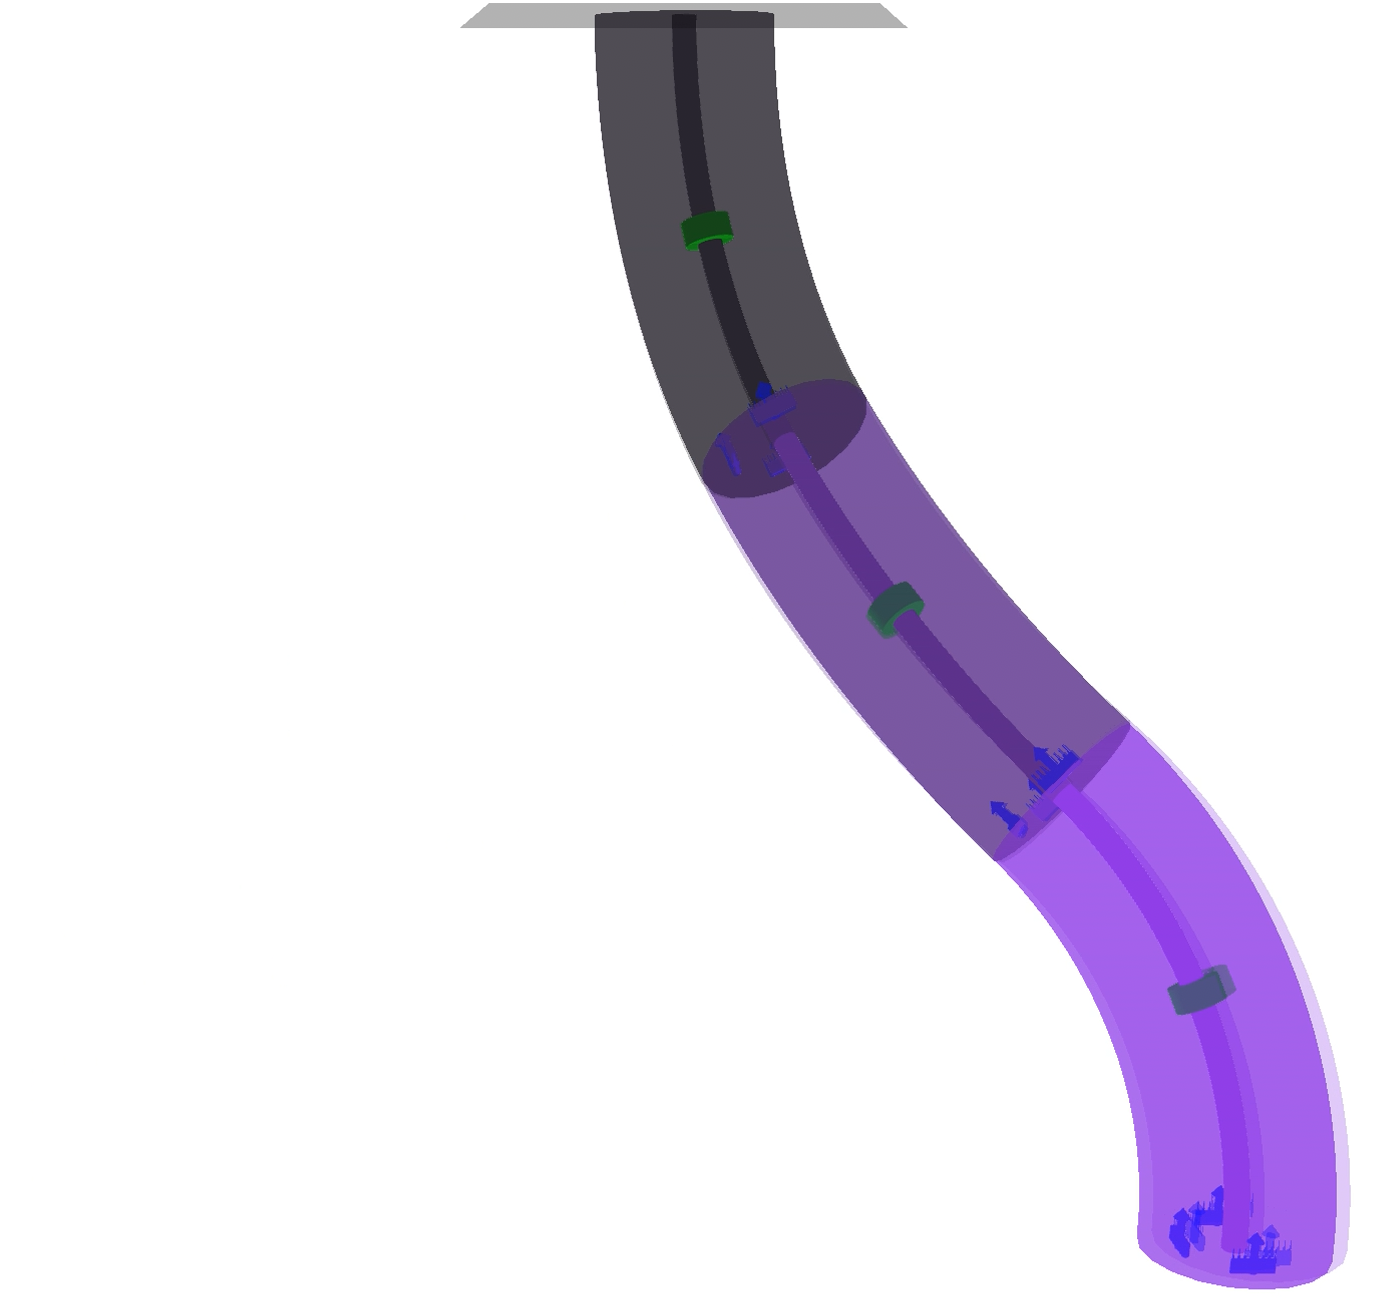
\includegraphics[width=0.161\textwidth]{promasens/figures/simulation_sequences/pcc_simulated_sensor_failure/simulated_sensor_failure_t=6s_cropped.png}}
  \hfill
  \subfigure[$t=\SI{8}{s}$]{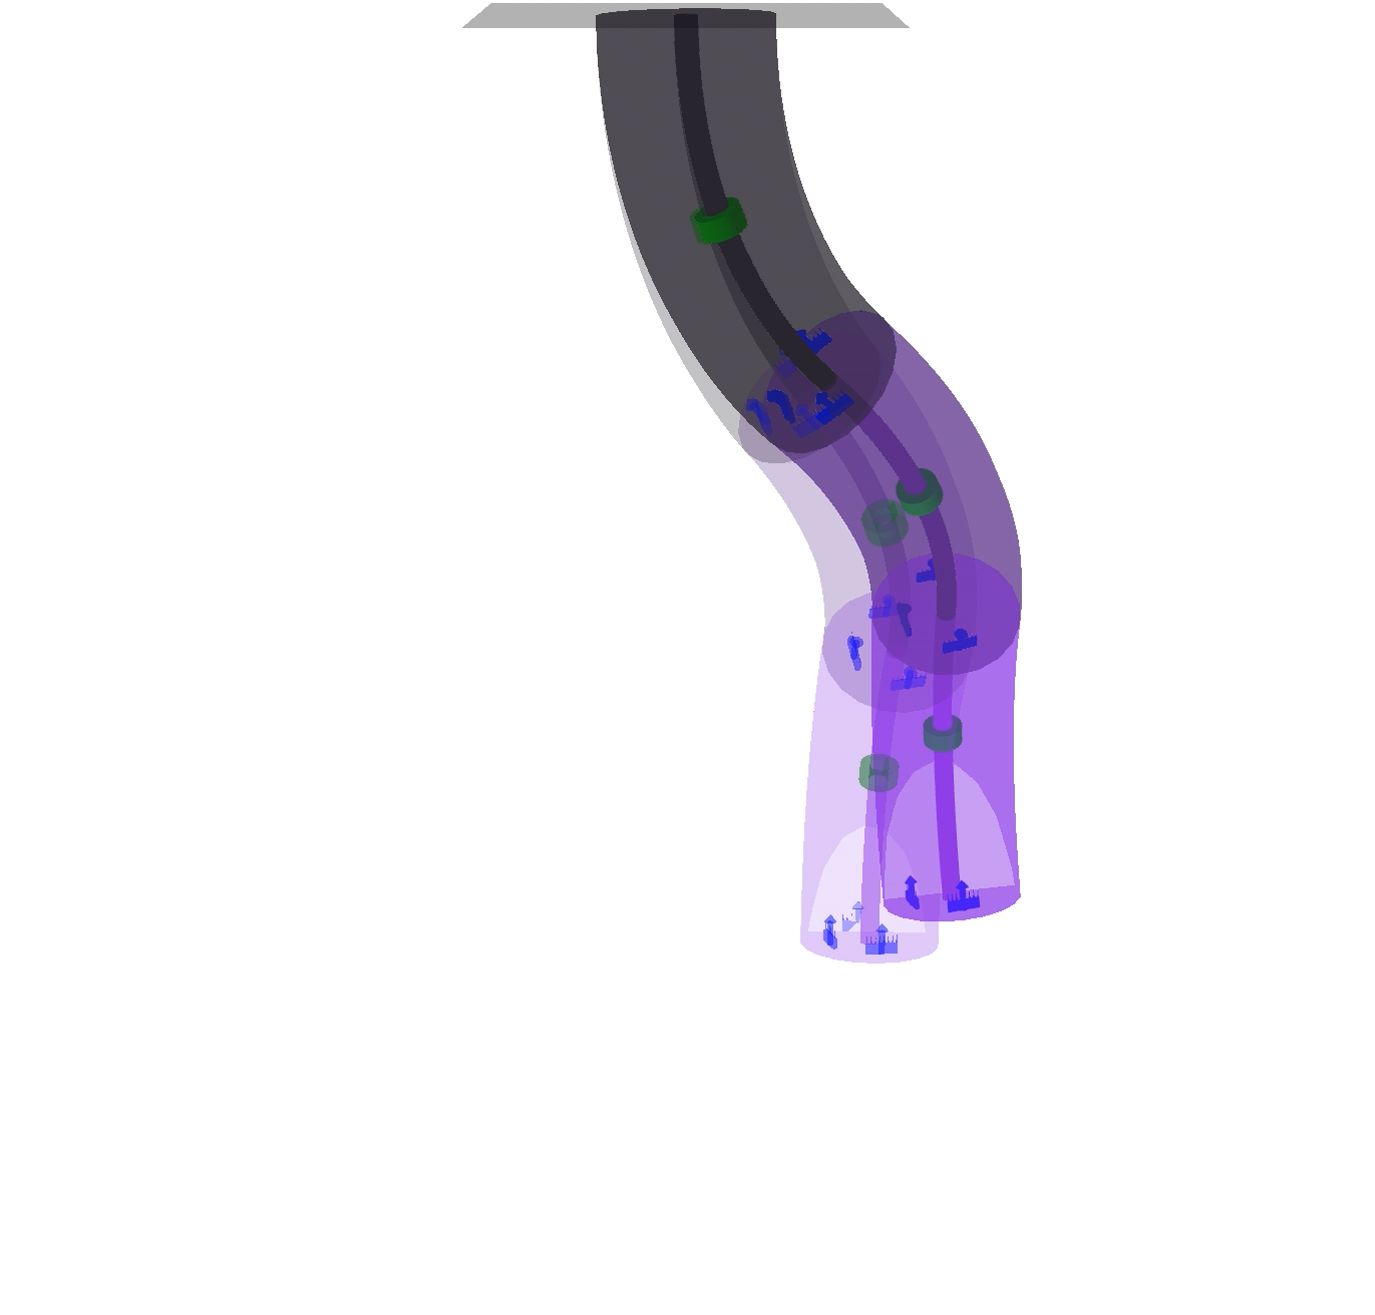
\includegraphics[width=0.161\textwidth]{promasens/figures/simulation_sequences/pcc_simulated_sensor_failure/simulated_sensor_failure_t=8s_cropped.png}}
  \hfill
  \subfigure[$t=\SI{10}{s}$]{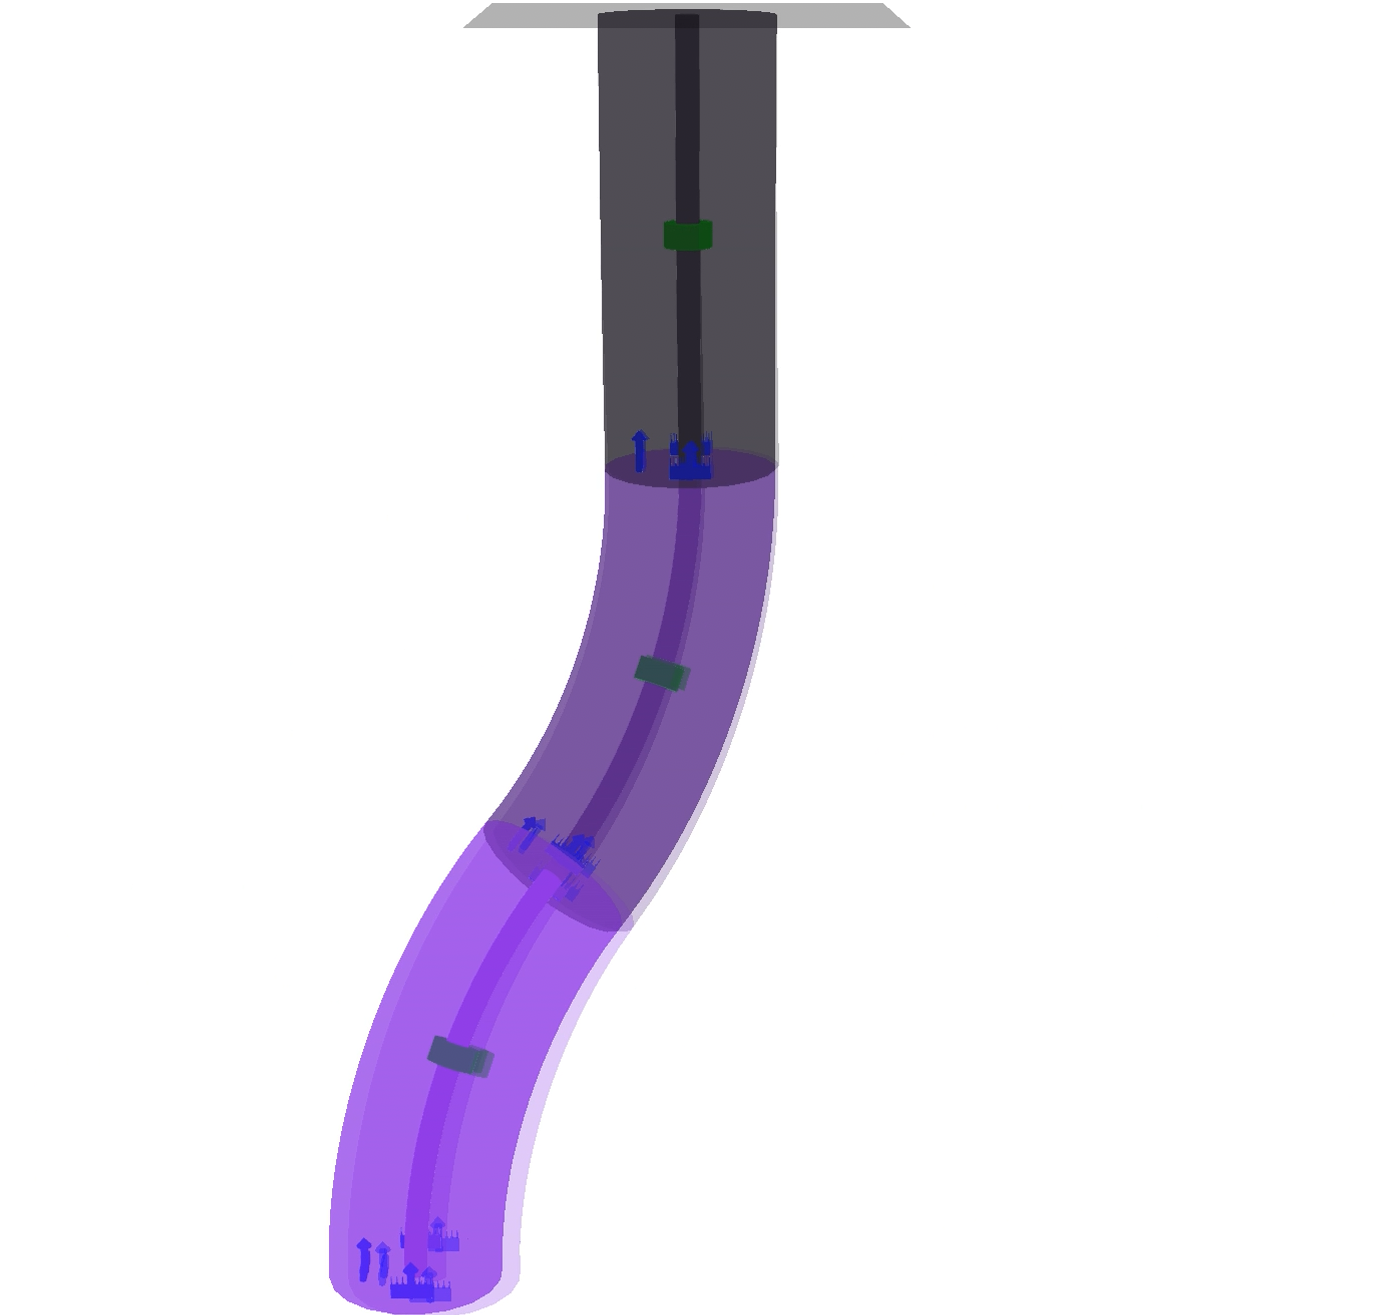
\includegraphics[width=0.161\textwidth]{promasens/figures/simulation_sequences/pcc_simulated_sensor_failure/simulated_sensor_failure_t=10s_cropped.png}}
  % 1375px x 1315px
  \caption{Sequence of stills for simulated sensor failure as shown in Figure~\ref{fig:promasens:simulated_sensor_failure}: the number of sensors per segment, which are rendered in blue, is reduced from four to three at $t=\SI{5}{s}$. We visualize the ground-truth shape of the soft robot with full opacity and the estimated configuration with slight transparency. The magnets are rendered in green and the three segments are visualized in a color sequence from black to violet.}
  \label{fig:promasens:simulation_sequences}
\end{figure*}

\subsection{Optimization}
We optimize the configuration variables $\hat{q}_i = (\hat{\Delta}_{x,i}, \hat{\Delta}_{y,i}, \hat{\delta} L_{i})^\mathrm{T}$ for each segment to minimize the sensor measurement prediction loss as defined in \eqref{eq:promasens:proprioception_loss}.
The optimization strategy solely relies on gradient descent and uses the best solution from the last time step $\hat{q}^*(t-1)$ as an initialization $\hat{q}_0(t)$. For the first time step of the trajectory, we initialize with the ground truth.
We use a step size $\gamma = 3.5 \cdot 10^{-4}$, $3 \cdot 10^{-3}$, and $2 \cdot 10^{-3}$ during gradient descent for a one-segment, two-segment and three-segment robot respectively. For all robots with more than one segment, the step size is reduced by a factor of ten when optimizing the elongation. The momentum $\mu$ is $0.3$ for all trials and we perform $20$ gradient descent iterations for each time step.

\subsection{Evaluation}\label{sub:promasens:pcc_simulations:evaluation}
We evaluate the performance of our method at estimating the configuration of the segment by computing a relative Root Mean-Squared Error (RMSE) metric with respect to the ground-truth configuration $q(t)$ for each configuration variable separately
\begin{equation}\label{eq:promasens:relative_RMSE}
\begin{split}
    e_{q_\star} = \frac{\sqrt{\sum_{t=0}^{n_\mathrm{t}} \left ( \hat{q}_\star(t) - q_\star(t) \right )^2}}{\sqrt{n_\mathrm{t}} \; D_{q_\star}},\\
    % e_{\Delta_y} = \frac{\sqrt{\sum_{t=0}^{n_\mathrm{t}} \left ( \hat{\Delta}_y(t) - \Delta_y(t) \right )^2}}{\sqrt{n_\mathrm{t}} \; L_{\Delta_y}},\\
    % e_{\delta L} = \frac{\sqrt{\sum_{t=0}^{n_\mathrm{t}} \left ( \delta \hat{L}(t) - \delta L(t) \right )^2}}{\sqrt{n_\mathrm{t}} \; L_{\delta L}},
\end{split}
\end{equation}
where $n_\mathrm{t}$ is the number of discrete time-steps and $D_{q_\star}$ is the dynamic range of each configuration variable between the maximum and minimum value in the test set.
All simulations are evaluated on a full lemniscate trajectory, which is very similar to what is plotted based on experimental data in Fig.~\ref{fig:promasens:t3_viz}. The maximum bending angle of this trajectory is \SI{45}{\degree} and the elongation of the segment follows a cosine wave with a minimum and maximum at \SI{1.25}{\percent} and \SI{3.75}{\percent} respectively.

\subsection{Results}\label{sub:promasens:simulation_pcc_results}
We present all simulation results in Tab.~\ref{tab:results_pcc_simulations}.
In the first section, robots with one to three segments, which all exhibit a nominal sensor placement, are considered separately. Neural networks are trained separately for each of these robots, as the input dimension needs to be adjusted to the number of magnets.
% We plot the configuration estimates for the three-segment robot in Fig.~\ref{fig:promasens:simulations_plot}.
The results show that the method works well for robots with 1-3 segments. It can be observed that the estimation error is usually lower for the distal segment(s).

Next, the number of sensors $n_\mathrm{s}$ is varied for a three-segment robot. We always apply a symmetrical placement of the sensors in the tip plane of each segment. In the first trial, two sensors are mounted in the tip plane of each segment opposite to each other (6 sensors in total). While the bending along $\Delta_{x,i}$ and the elongation of the segments $\delta L_i$ can still be estimated, the setup does not contain sufficient information to accurately determine the bending into $\Delta_{y,i}$.
While the nominal case of nine sensors in total already achieves relative RMSEs in the range of \SI{1.6}{\percent} to \SI{6}{\percent}, the proprioception performance can be slightly improved by adding more sensors.
% Recall that no re-training of the neural network is required when adding or removing sensors.
We emphasize that the neural networks are not retrained when adding or removing sensors.
In Figures~\ref{fig:promasens:simulated_sensor_failure} and \ref{fig:promasens:simulation_sequences}, we plot the proprioceptive performance of a three-segment robot with four sensors per segment. Then, we simulated a failure of the 4th, 8th, and 12th sensor at \SI{5}{s} by removing these sensor measurements from \eqref{eq:promasens:gradient_descent} (i.e. the gradient descent). Our method is able to adapt without re-training and leverage the nominal redundancy of sensor measurements, as three sensors per segment are sufficient for shape estimation.

Then, two adjusted sensor placements are investigated, while keeping the neural network weights constant. First, the sensors are tilted from the nominal case of pointing along the local z-axis by $\psi_\mathrm{s} = \SI{10}{\degree}$ towards the inside. In a separate simulation, the sensors are moved radially from nominally \SI{13}{mm} to \SI{16}{mm}. As the results show, the configuration of all three segments can still be estimated accurately with a mean error of \SI{3.3}{\percent}.

Finally, an earth's magnetic field of magnitude \SI{0.065}{mT} is added. A separate neural network is trained on a training set with randomly sampled magnetic field vector directions $n_\mathrm{e}$. As the last section of Tab.~\ref{tab:results_pcc_simulations} demonstrates, the methodology is able to adapt to any earth's magnetic field direction by leveraging the $\lambda_j$ input parameter.

% \subsection{Synthetic results}\label{sub:promasens:synthetic_results}
% We initially verify and quantitatively compare our method with an end-to-end trained neural network using a synthetic sensor measurement model: \textcolor{red}{Insert citation why we are using this synthetic sensor measurement model and also describe the \gls{NN} and how it differs from \gls{NN} from our method}
% \begin{equation}
%     u_j = \sum_{k=1}^{n_\mathrm{m}} \frac{1000}{d_{jk}^2} \cdot \cos( \theta_{jk}) \cdot \cos( \beta_{jk}) + n_u
% \end{equation}

% Alternatively, we implement a more realistic, analytical 2D model for the magnetic flux intensity of one magnet $k$ measured by sensor $j$. As our segment is axially symmetric, we can a 2D magnetic flux model in the plane of the angle $\theta_{jk}$. Referring to \eqref{eq:promasens:d_jk} and \eqref{eq:promasens:theta_jk}, we define the radial and axial distance between the magnet and the sensor as:
% \begin{equation}
%     d_{a,jk} = \cos(\theta_{jk}) \cdot d_{jk} \qquad d_{r,jk} = \sin(\theta_{jk}) \cdot d_{jk}
% \end{equation}
% For a magnet with thickness $h_m$ and of diameter $D_m$ in a medium with a relative magnetic permeability $\mu_o$ (for air $1.00000037$) and $M_a$ the surface magnetization magnitude of the magnet, we can define the magnetic field vector components in the cylindrical coordinate system of the magnet $jk$ as~\cite{furlani2001permanent, ozel2015precise}:
% \begin{equation}\scriptsize
% \begin{split}
%     B^a(d_a, d_r) = \frac{\mu_0 M_x}{2 \pi} \Bigg ( & \quad \arctan \frac{2 h_m \cdot (d_a + D_m)}{(d_a + D_m)^2 + d_r^2 - h_m^2} \\ 
%     & - \arctan \frac{2 h_m \cdot (d_a - D_m)}{(d_a - D_m)^2 + d_r^2 - h_m^2} \Bigg ),\\
%     B^r(d_a, d_r) = \frac{\mu_0 M_x}{2 \pi} \Bigg ( & \quad \ln \frac{(d_a + D_m)^2 + (d_r - h_m)^2 }{(d_a + D_m)^2 + (d_r + h_m)^2} \\ 
%     & - \ln \frac{(d_a - D_m)^2 + (d_r - h_m)^2 }{(d_a - D_m)^2 + (d_r + h_m)^2}  \Bigg ).
% \end{split}
% \end{equation}
% We rotate the translation between the magnet and the sensor into the magnet frame $\{S_{\mathrm{m}_k}\}$ and project it into the local x-y plane:
% \begin{equation}
%     t_{\mathrm{m}_k,xy}^{jk} = 
%     \mathrm{diag}(\begin{bmatrix} 1 & 1 & 0 \end{bmatrix}) 
%     \cdot (R_{i-1}^{\mathrm{m}_k})^{\mathrm{T}} \cdot t_{i-1}^{jk},
% \end{equation}
% which allows us to define the magnetic field vector in the frame $\{ S_{\mathrm{m}_k} \}$:
% \begin{equation}
%     B_{\mathrm{m}_k}^{jk} = 
%     \begin{bmatrix}
%         \frac{x^{t_{jk}}_{\mathrm{m}_k,xy}}{\lVert  t_{\mathrm{m}_k,xy}^{jk} \rVert} \cdot B^{r,jk} & \frac{y^{t_{jk}}_{\mathrm{m}_k,xy}}{\lVert  t_{\mathrm{m}_k,xy}^{jk} \rVert} \cdot B^{r,jk} & B^{a,jk}
%     \end{bmatrix}^{\mathrm{T}}.
% \end{equation}
% Next, we compute the expected sensor measurement $u_j$ using the scalar projection of the magnetic field vector $B_{i-1}^{jk}$ along the sensor measurement unit vector $\{ \hat{o}_{\mathrm{s}_j} \}_{i-1}$ with the dot product as:
% \begin{equation}
%     u_j = \sum_{k=1}^{n_\mathrm{m}} \left ( R_{i-1}^{\mathrm{m}_k} \cdot B_{\mathrm{m}_k}^{jk} \right ) \cdot \{ \hat{o}_{\mathrm{s}_j} \}_{i-1}
% \end{equation}

% We apply both input and process Gaussian noise to pose a realistic challenge for both proprioception methods.
% \textcolor{red}{Please insert the correct noise values here:}
% We add the process noise $n_u \sim \mathcal{N}\left(\SI{0.2}{V}, \SI{0.5}{V} \right)$ to the target sensor measurement $u$ and the inputs noise $n_d \sim \mathcal{N}\left(\SI{0.2}{m}, \SI{0.5}{m} \right)$, $n_\theta \sim \mathcal{N}\left(\SI{0.2}{\degree}, \SI{0.5}{\degree} \right)$ and $n_\beta \sim \mathcal{N}\left(\SI{0.2}{\degree}, \SI{0.5}{\degree} \right)$ before $\Bar{\xi}$ is passed to the neural network:
% \begin{equation}
%     \Bar{\xi}_{jk} = \xi_{jk} + 
%     \begin{bmatrix}
%     n_d & n_\theta & n_\beta
%     \end{bmatrix}^\mathrm{T}
% \end{equation}

\section{Affine Curvature Simulations}\label{sec:promasens:ac_simulations}
To demonstrate the efficacy of the proposed method for higher-order kinematic models than \gls{PCC}, we also conduct simulations of an \gls{AC} soft robot.
The \gls{AC} kinematic parametrization~\citep{della2020soft} has been shown capable of representing the shape of soft tentacles~\citep{stella2022experimental, stella2023piecewise} and provides a continuous function $\kappa = \kappa_0 + \kappa_1 \: v$ to describe the curvature of the soft robot, where $\kappa_0$, $\kappa_1$ are two configuration variables and $v \in [0, 1]$ is the backbone coordinate. We allow for movement in 3D space by also specifying an azimuth bending angle $\phi$ and the elongation $\delta L$.
Please refer to Section~\ref{sub:promasens:kinematic_model_ac} for more implementation details about the \gls{AC} model.


\subsection{Simulation Setup}\label{sub:promasens:ac_simulations:simulation_setup}
We use the same simulation setup as described in Section~\ref{sub:promasens:pcc_simulations:simulation_setup}. 
Therefore, we report in the following only the implemented modifications to simulate an \gls{AC} soft robot in Magpylib~\citep{magpylib2020}.
Namely, we consider one \gls{AC} segment of length $L_{0,i} = \SI{200}{mm}$ with in total $n_\mathrm{s} = 9$ magnetic sensors. 
The sensors are placed on three separate cylindrical planes at distances $d_{\mathrm{s}_\mathrm{a}}$ of \SI{0}{mm}, \SI{100}{mm}, and \SI{200}{mm} from the base of the robot. In each plane, the three sensors are spaced at an angle of \SI{120}{\degree} and at a radial distance $d_{\mathrm{s}_\mathrm{r}} = \SI{13}{mm}$ from the backbone, as it can be seen in Fig.~\ref{fig:promasens:ac_simulations:inference_sequences}.
Two ring magnets are positioned at a distance of \SI{50}{mm} and \SI{150}{mm} from the robot's base, respectively.

\begin{figure}[hbt]
  \centering
  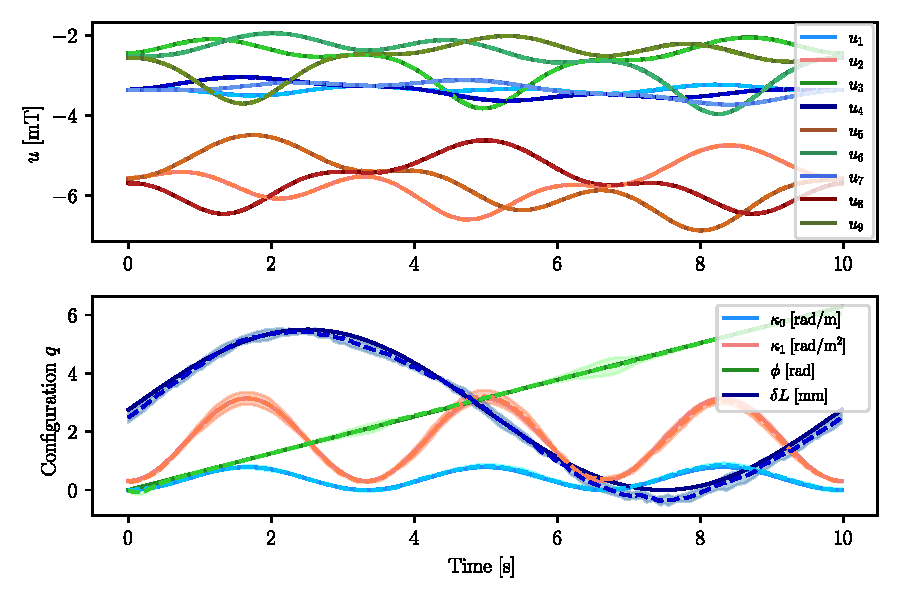
\includegraphics[width=0.8\columnwidth]{promasens/figures/simulation_results/ac/affine_curvature_inference_v2_cropped.pdf}
  \caption{Sensor measurement predictions (top) and configuration estimates (bottom) for an \gls{AC} segment with nine magnetic sensors. We plot the ground-truth values $u$ and $q$ in solid, the estimate $\hat{u}$ and $\hat{q}$ as a mean over three random seeds with dashed lines and the standard deviation as an error band. The random seed determines the initialization of the neural network weights at the start of the training.}
  \label{fig:promasens:ac_simulations:inference_plot}
\end{figure}

\begin{figure*}[hbt]
  \centering
  \subfigure[$t=\SI{0}{s}$]{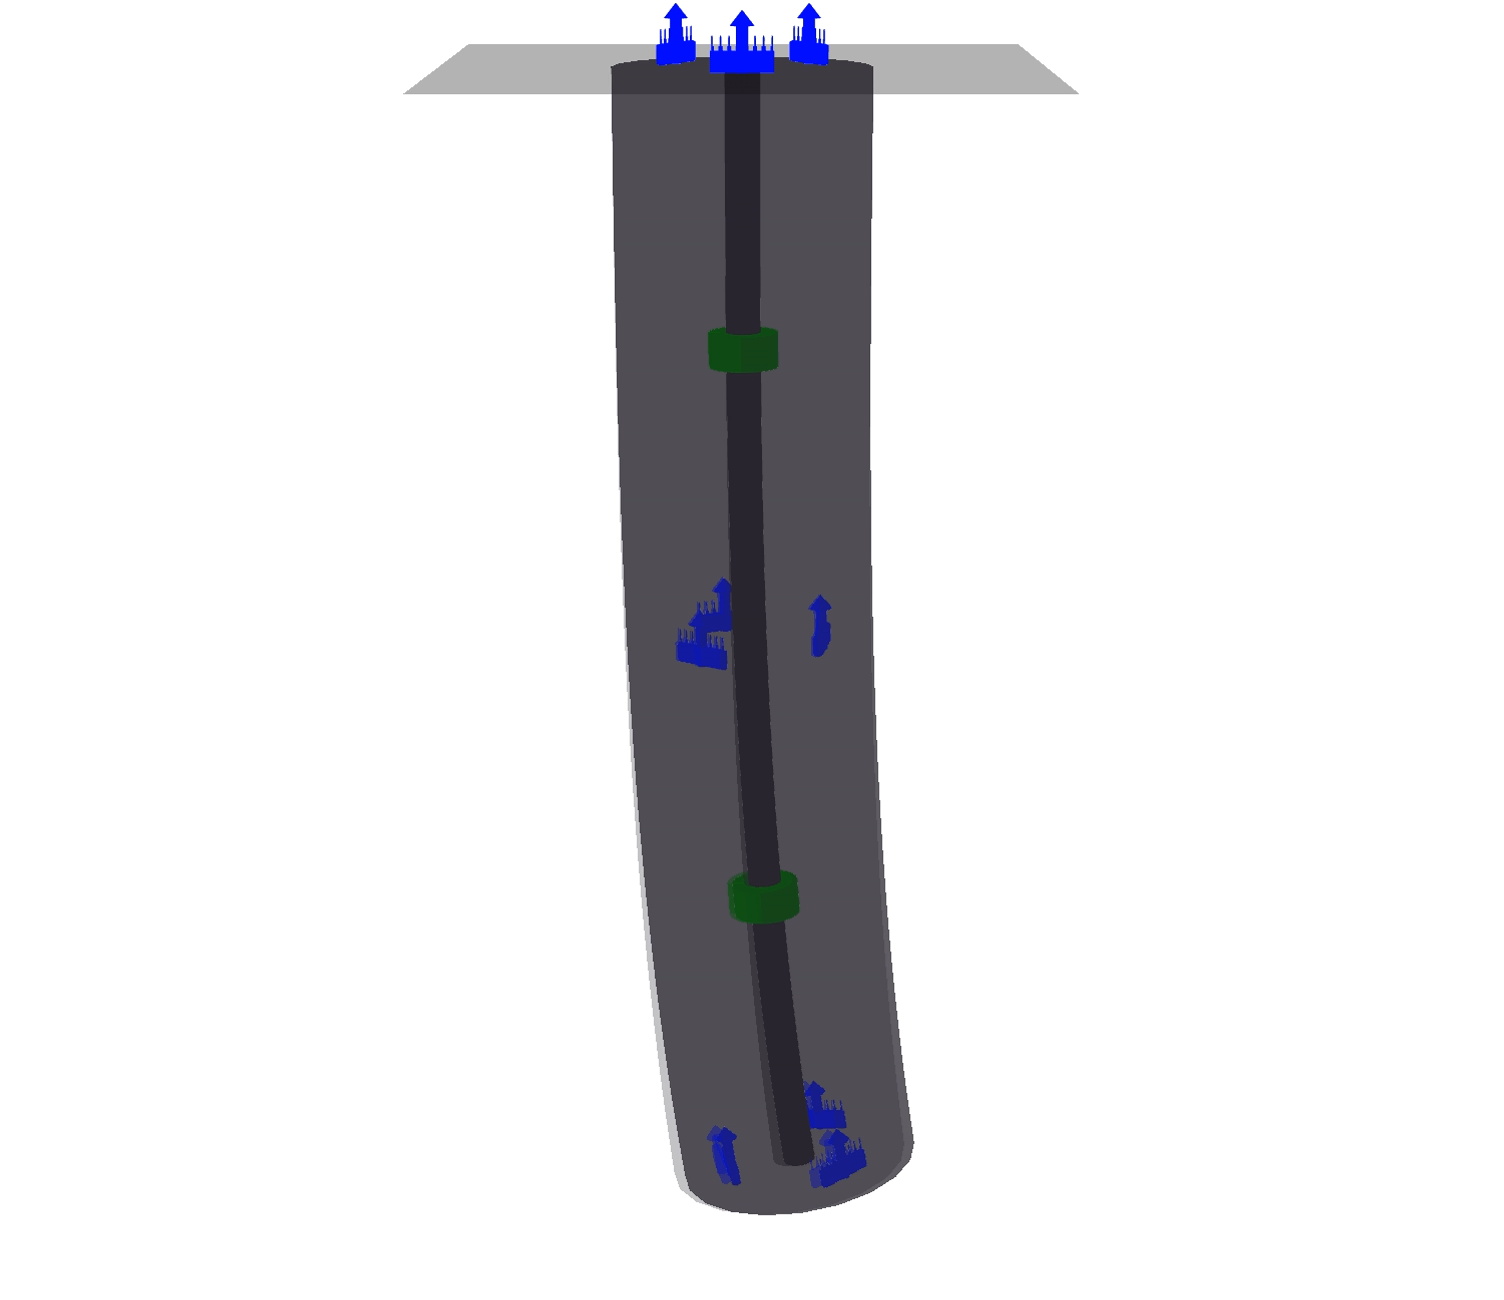
\includegraphics[width=0.161\textwidth]{promasens/figures/simulation_sequences/ac_flower_trajectory/affine_curvature_flower_t=0s_cropped.png}}
  \hfill
  \subfigure[$t=\SI{2}{s}$]{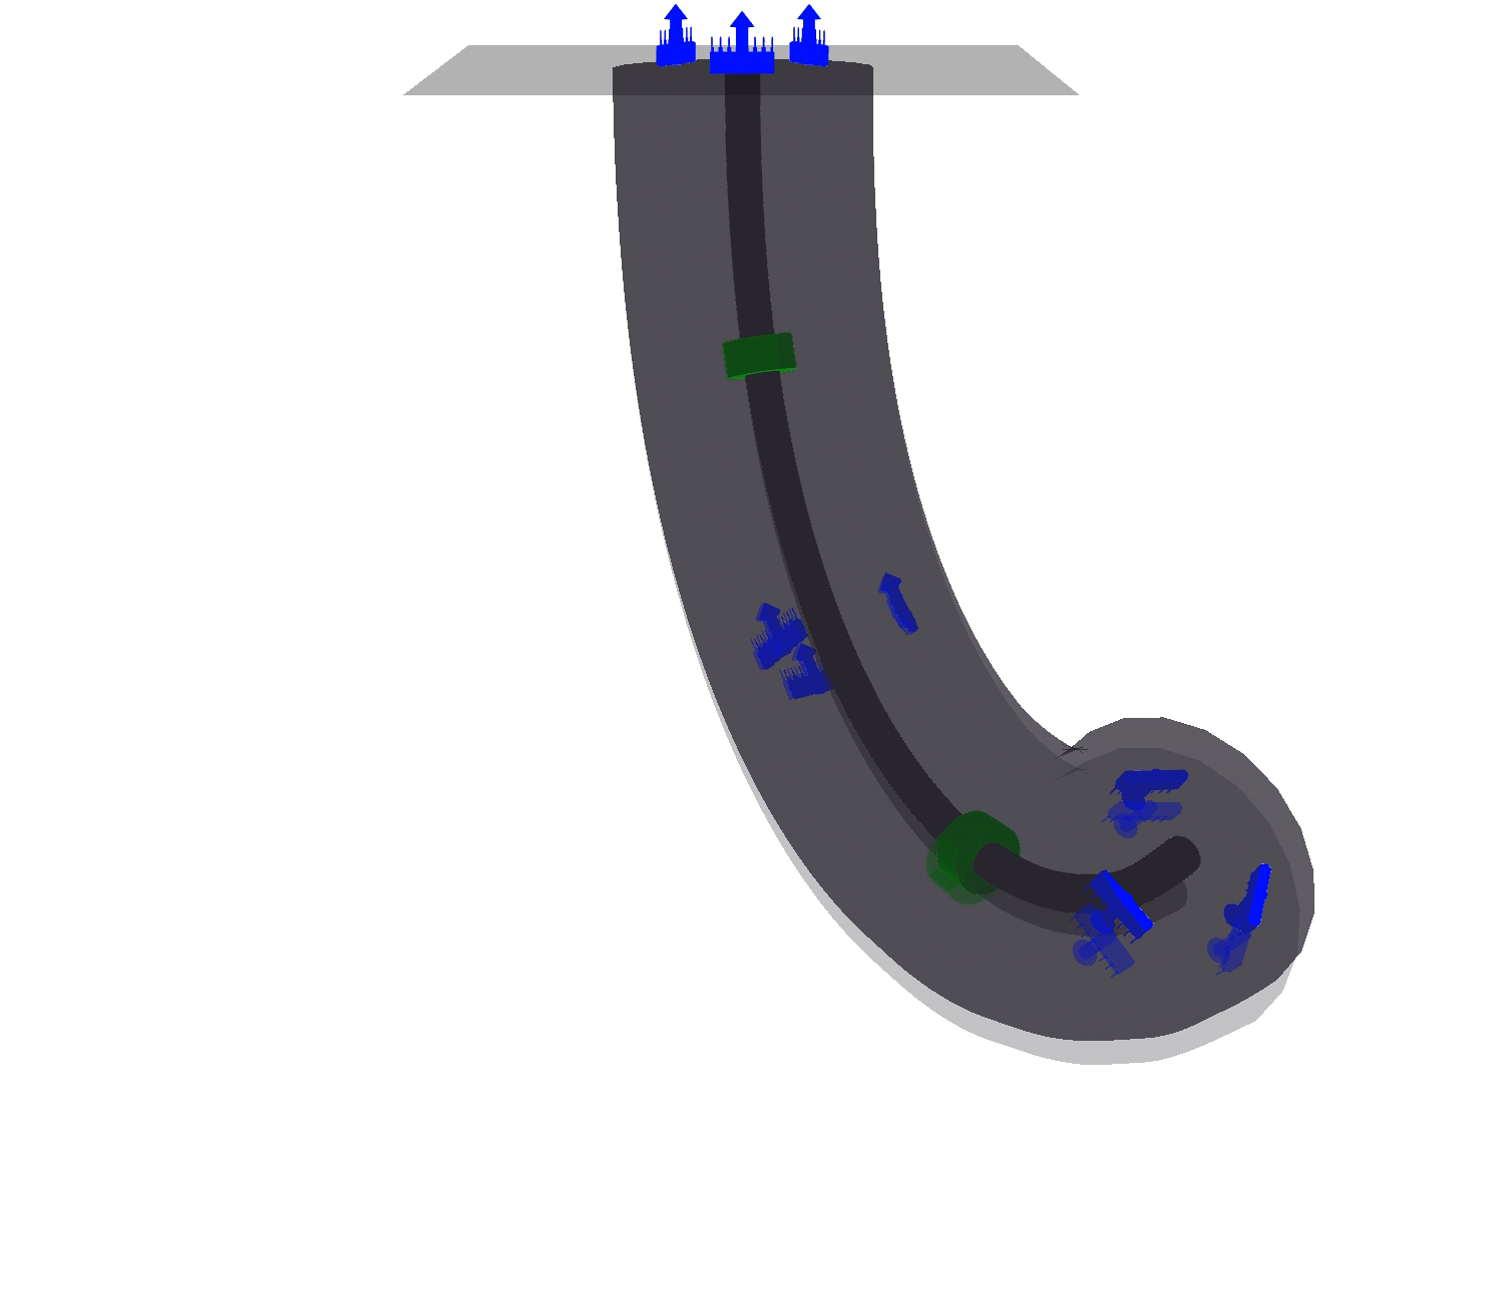
\includegraphics[width=0.161\textwidth]{promasens/figures/simulation_sequences/ac_flower_trajectory/affine_curvature_flower_t=2s_cropped.png}}
  \hfill
  \subfigure[$t=\SI{4}{s}$]{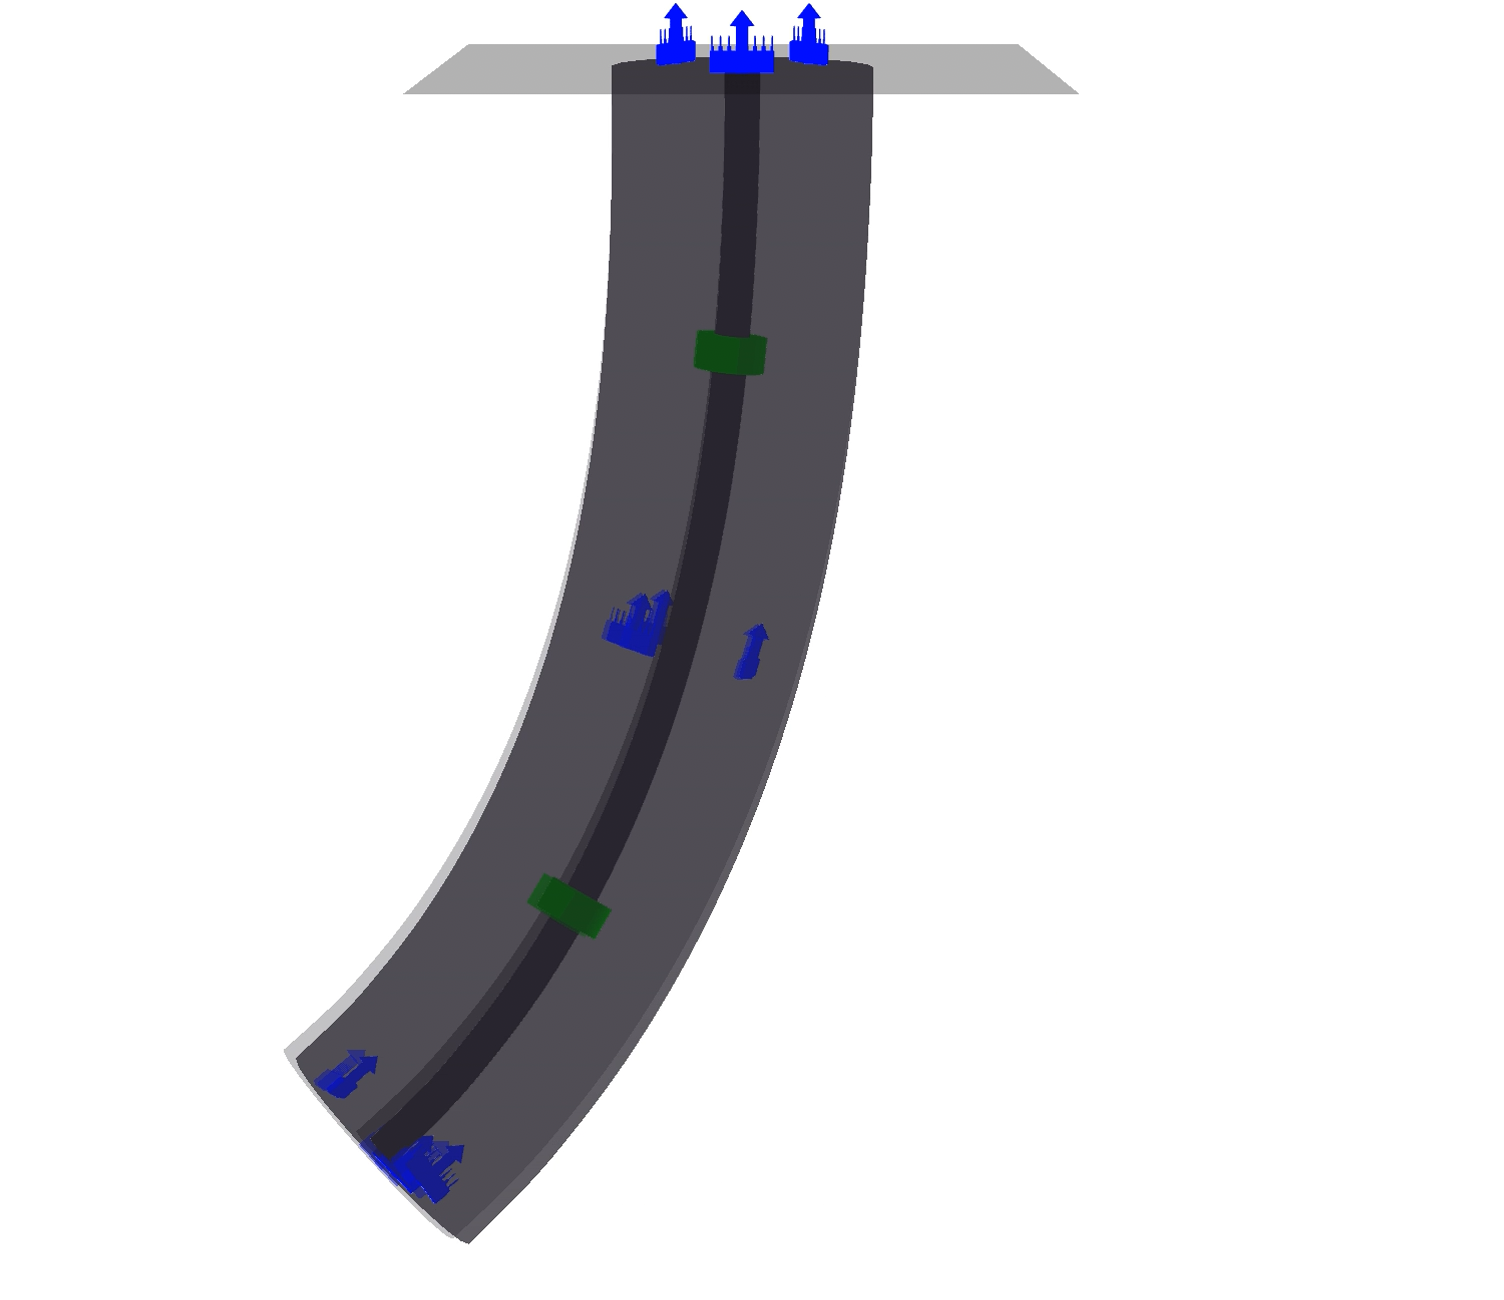
\includegraphics[width=0.161\textwidth]{promasens/figures/simulation_sequences/ac_flower_trajectory/affine_curvature_flower_t=4s_cropped.png}}
  \hfill
  \subfigure[$t=\SI{6}{s}$]{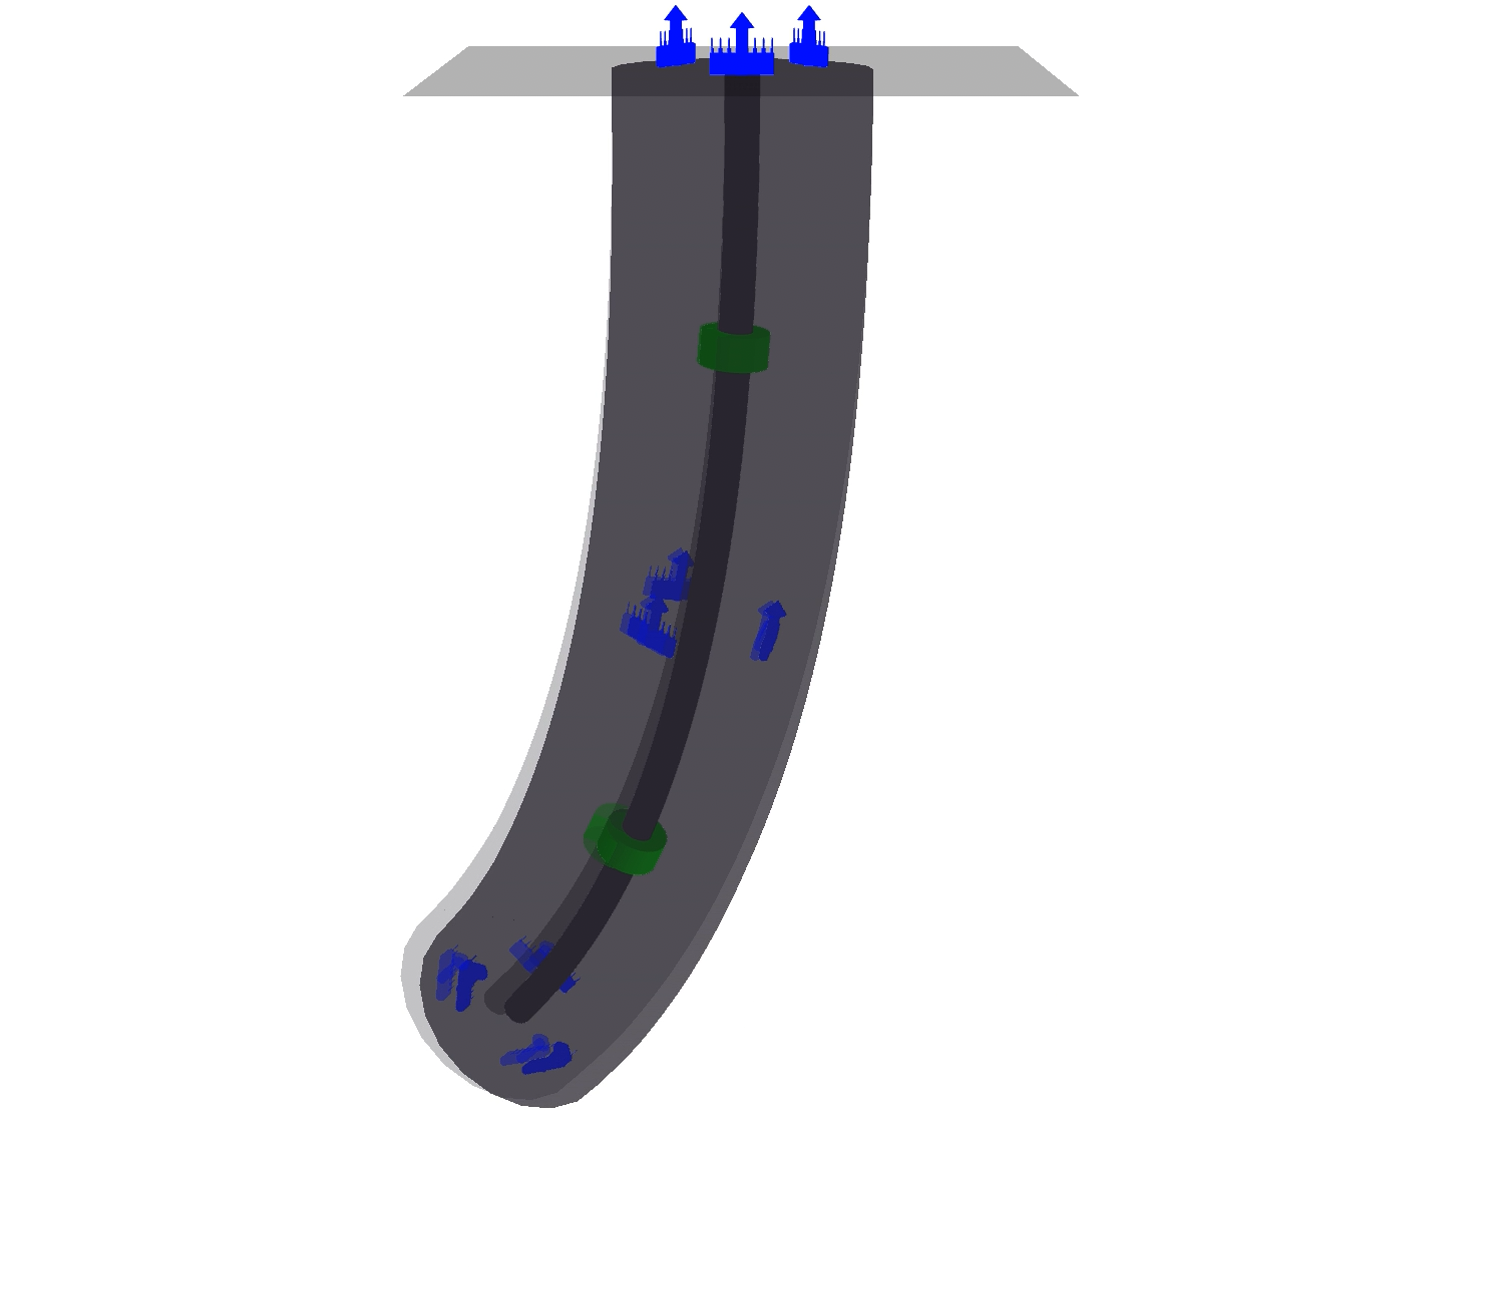
\includegraphics[width=0.161\textwidth]{promasens/figures/simulation_sequences/ac_flower_trajectory/affine_curvature_flower_t=6s_cropped.png}}
  \hfill
  \subfigure[$t=\SI{8}{s}$]{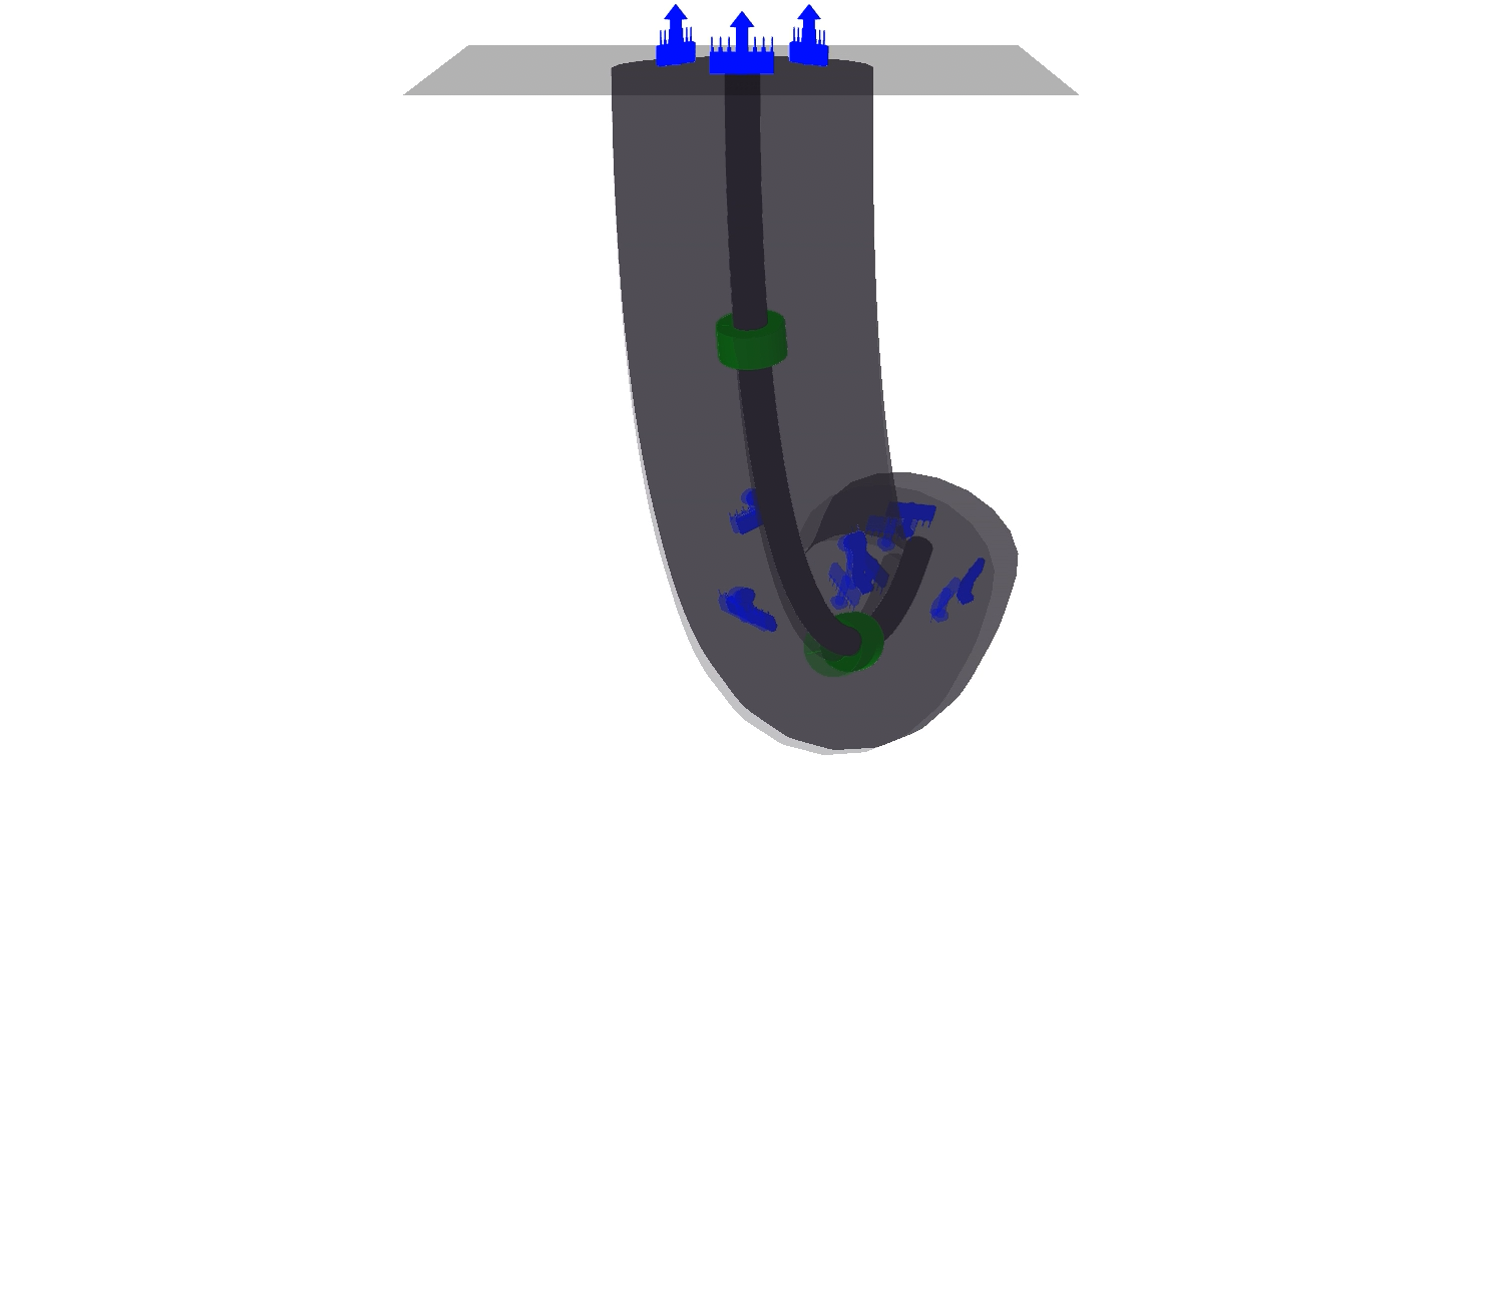
\includegraphics[width=0.161\textwidth]{promasens/figures/simulation_sequences/ac_flower_trajectory/affine_curvature_flower_t=8s_cropped.png}}
  \hfill
  \subfigure[$t=\SI{10}{s}$]{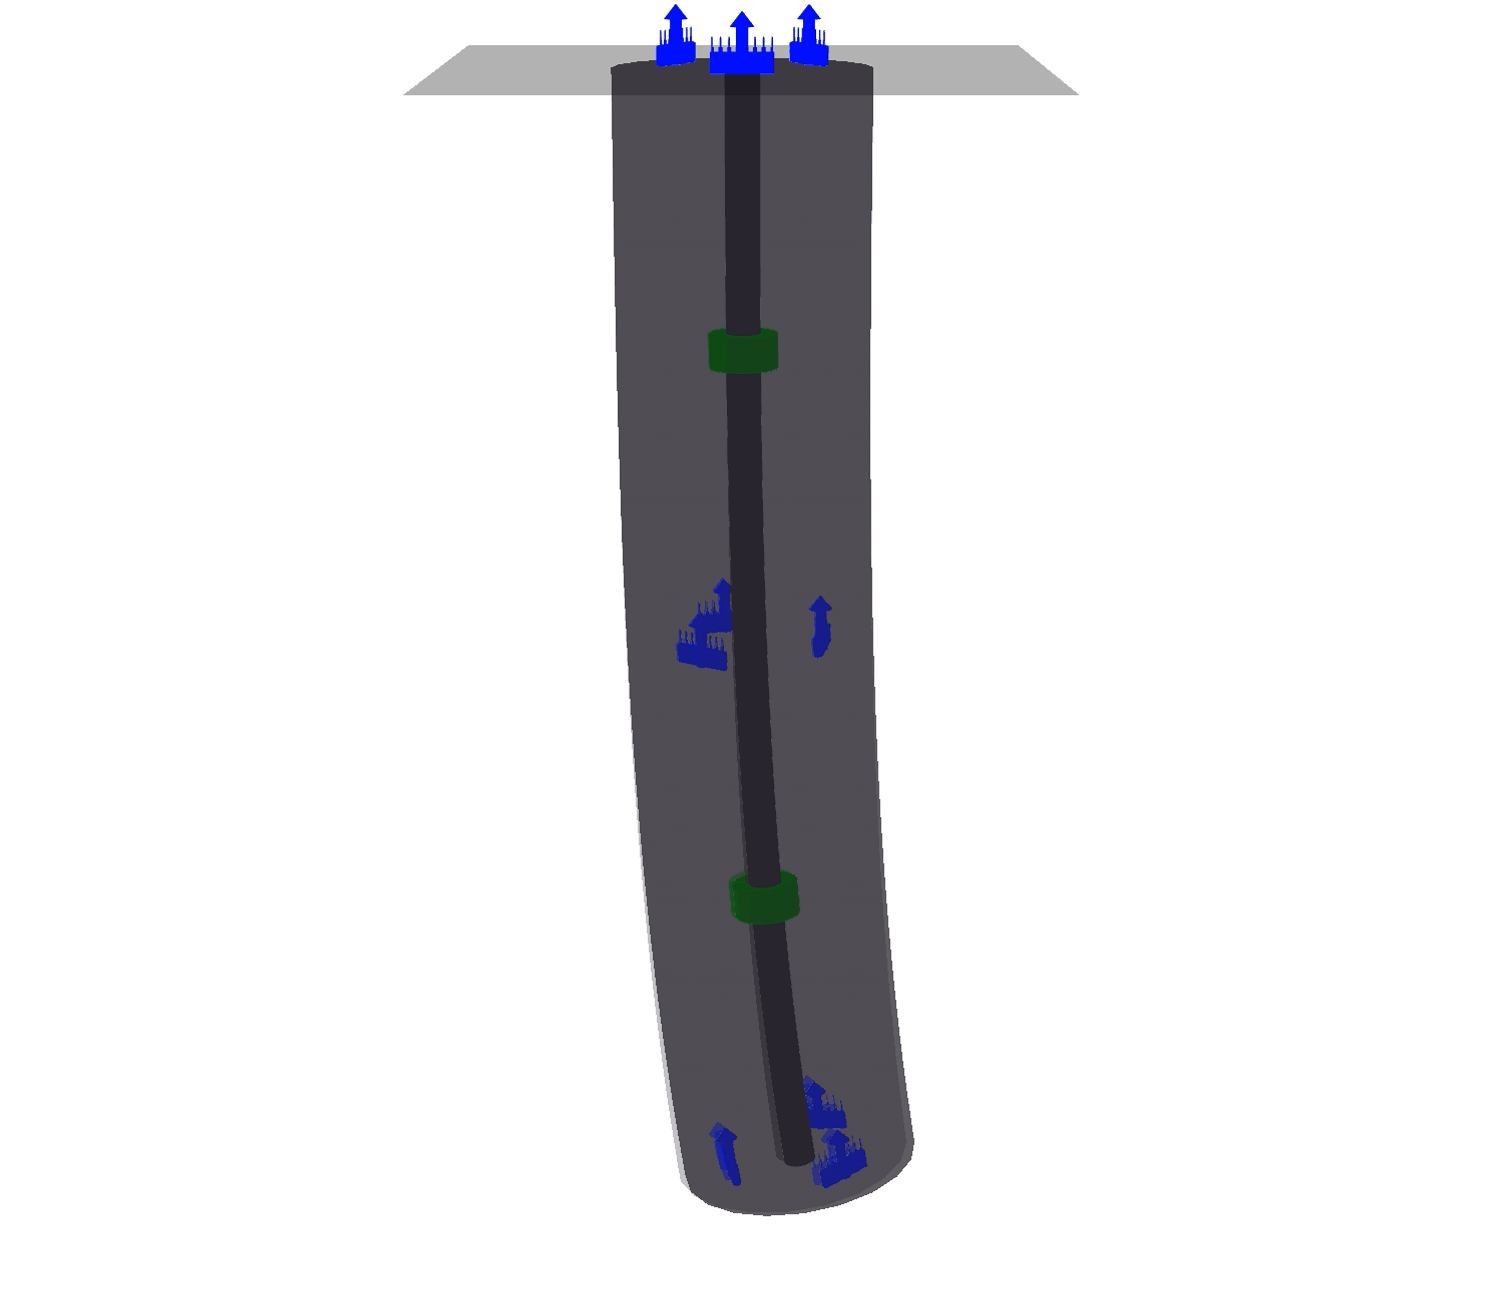
\includegraphics[width=0.161\textwidth]{promasens/figures/simulation_sequences/ac_flower_trajectory/affine_curvature_flower_t=10s_cropped.png}}
  % 1504 x 1400px
  \caption{Sequence of stills for a simulated \gls{AC} robot. We visualize the ground-truth shape of the soft robot with full opacity and the estimated configuration with slight transparency. The two magnets are rendered in green and the nine sensors in blue.}
  \label{fig:promasens:ac_simulations:inference_sequences}
\end{figure*}

\subsection{Prediction Network and Optimization}\label{sub:promasens:ac_simulations:network_optimization}
We simulate \SI{120000}{} random configurations of the \gls{AC} robot to generate the training set. For this purpose, we sample the configuration variables from uniform distributions: the \gls{AC} parameters $\kappa_0 \in \mathcal{U}(0, \SI{0.942}{rad \per m})$, $\kappa_1 \in \mathcal{U}(0, \SI{3.770}{rad \per m^2})$, the azimuth angle $\phi \in \mathcal{U}(0, 2 \pi \: \si{rad})$, and the elongation $\delta L \in \mathcal{U}(0, \SI{6.6}{mm})$.
Before training, we randomly split off \SI{30}{\percent} of the training set for validation purposes.
We train a specialized neural network $f_{\pi_j(\xi_j)}$ for each sensor and use the same neural network architecture as in Section~\ref{sub:promasens:pcc_simulations:neural_network} with the exception of the addition of a final layer $y(x) = \mathrm{sign}(x) \: e^{|x|}$. 
The training runs for a total of $250$ epochs and uses the SWA~\citep{izmailov2018averaging} strategy with a learning rate of $0.01$. 
All other training hyperparameters are the same as in Section~\ref{sub:promasens:pcc_simulations:neural_network}.

The four configuration variables are optimized to minimize the loss between the predictions and simulated measurements of the nine sensors as defined in \ref{eq:promasens:proprioception_loss}.
For this optimization procedure, we employ gradient descent running at \SI{40}{Hz} with step sizes of $\gamma_{\kappa_0} = 1$, $\gamma_{\kappa_1} = 5$, $\gamma_{\phi} = 1$, and $\gamma_{\delta L} = 2 \cdot 10^{-4}$. The momentum is set to $\mu = 0.3$ and $20$ iterations are performed at each time step.

\subsection{Evaluation}\label{sub:promasens:ac_simulations:evaluation}
We evaluate the trained model on a flower trajectory of duration \SI{10}{s} and sample rate \SI{40}{Hz}. The evaluation trajectory has the following characteristics: $\kappa_0$ is actuated by a sinusoidal wave of frequency \SI{0.3}{Hz} in the range $[0, \frac{\pi}{4} \: \si{rad \per m}]$. Similarly, $\kappa_1$ is also varied through a sinusoidal function of the same frequency and has a dynamic range of $[0.1 \pi, \pi] \: \si{rad \per m^2}$.
The azimuth angle $\phi$ is linearly scaled from \SI{0}{rad} to $2 \pi \: \si{rad}$ over the duration of the trajectory.
Finally, $\delta L$ follows a sinusoidal sequence of frequency \SI{0.1}{Hz} in the range of $[0, 5.5] \: \si{mm}$.
We use the same evaluation metrics as first introduced in Section~\ref{sub:promasens:pcc_simulations:evaluation}.
We report the error as mean ± stdev and compute the statistics over three
different random seeds. The random seed determines the initialization of the neural network weights at the start of the training.

\subsection{Results}\label{sub:promasens:ac_simulations:results}
The trained neural networks achieve an RMSE error for predicting the magnetic sensor measurements of $0.025 \pm 0.002 \: \si{mT}$ on the test set.
When we run inference (see Fig.~\ref{fig:promasens:ac_simulations:inference_plot}) on the flower trajectory, the configuration variables can be estimated with an absolute RMSE of $e_{\kappa_0} = 0.042 \pm 0.005 \: \si{rad \per m}$, $e_{\kappa_1} = 0.11 \pm 0.04 \: \si{rad \per m^2}$, $e_{\phi} = 0.08 \pm 0.02 \: \si{rad}$, and $e_{\delta L} = 0.001 \pm 0.001 \: \si{mm}$. 
We state the relative RMSE errors for the configuration estimates as $e_{\kappa_0} = 5.4 \pm 0.7 \: \si{\percent}$, $e_{\kappa_1} = 4.0 \pm 1.4 \: \si{\percent}$, $e_{\phi} = 1.3 \pm 0.4 \: \si{\percent}$, and $e_{\delta L} = 3.8 \pm 1.6 \: \si{\percent}$.
In Fig.~\ref{fig:promasens:ac_simulations:inference_sequences}, we render at six different points along the trajectory the robot's shape according to the ground truth and estimated configurations, respectively.
The sequence qualitatively shows that our proposed method is able to estimate the affine curvature robot's shape very accurately.

\section{Experiments}\label{sec:promasens:experiments}
\begin{figure*}[hbt]
    \centering
    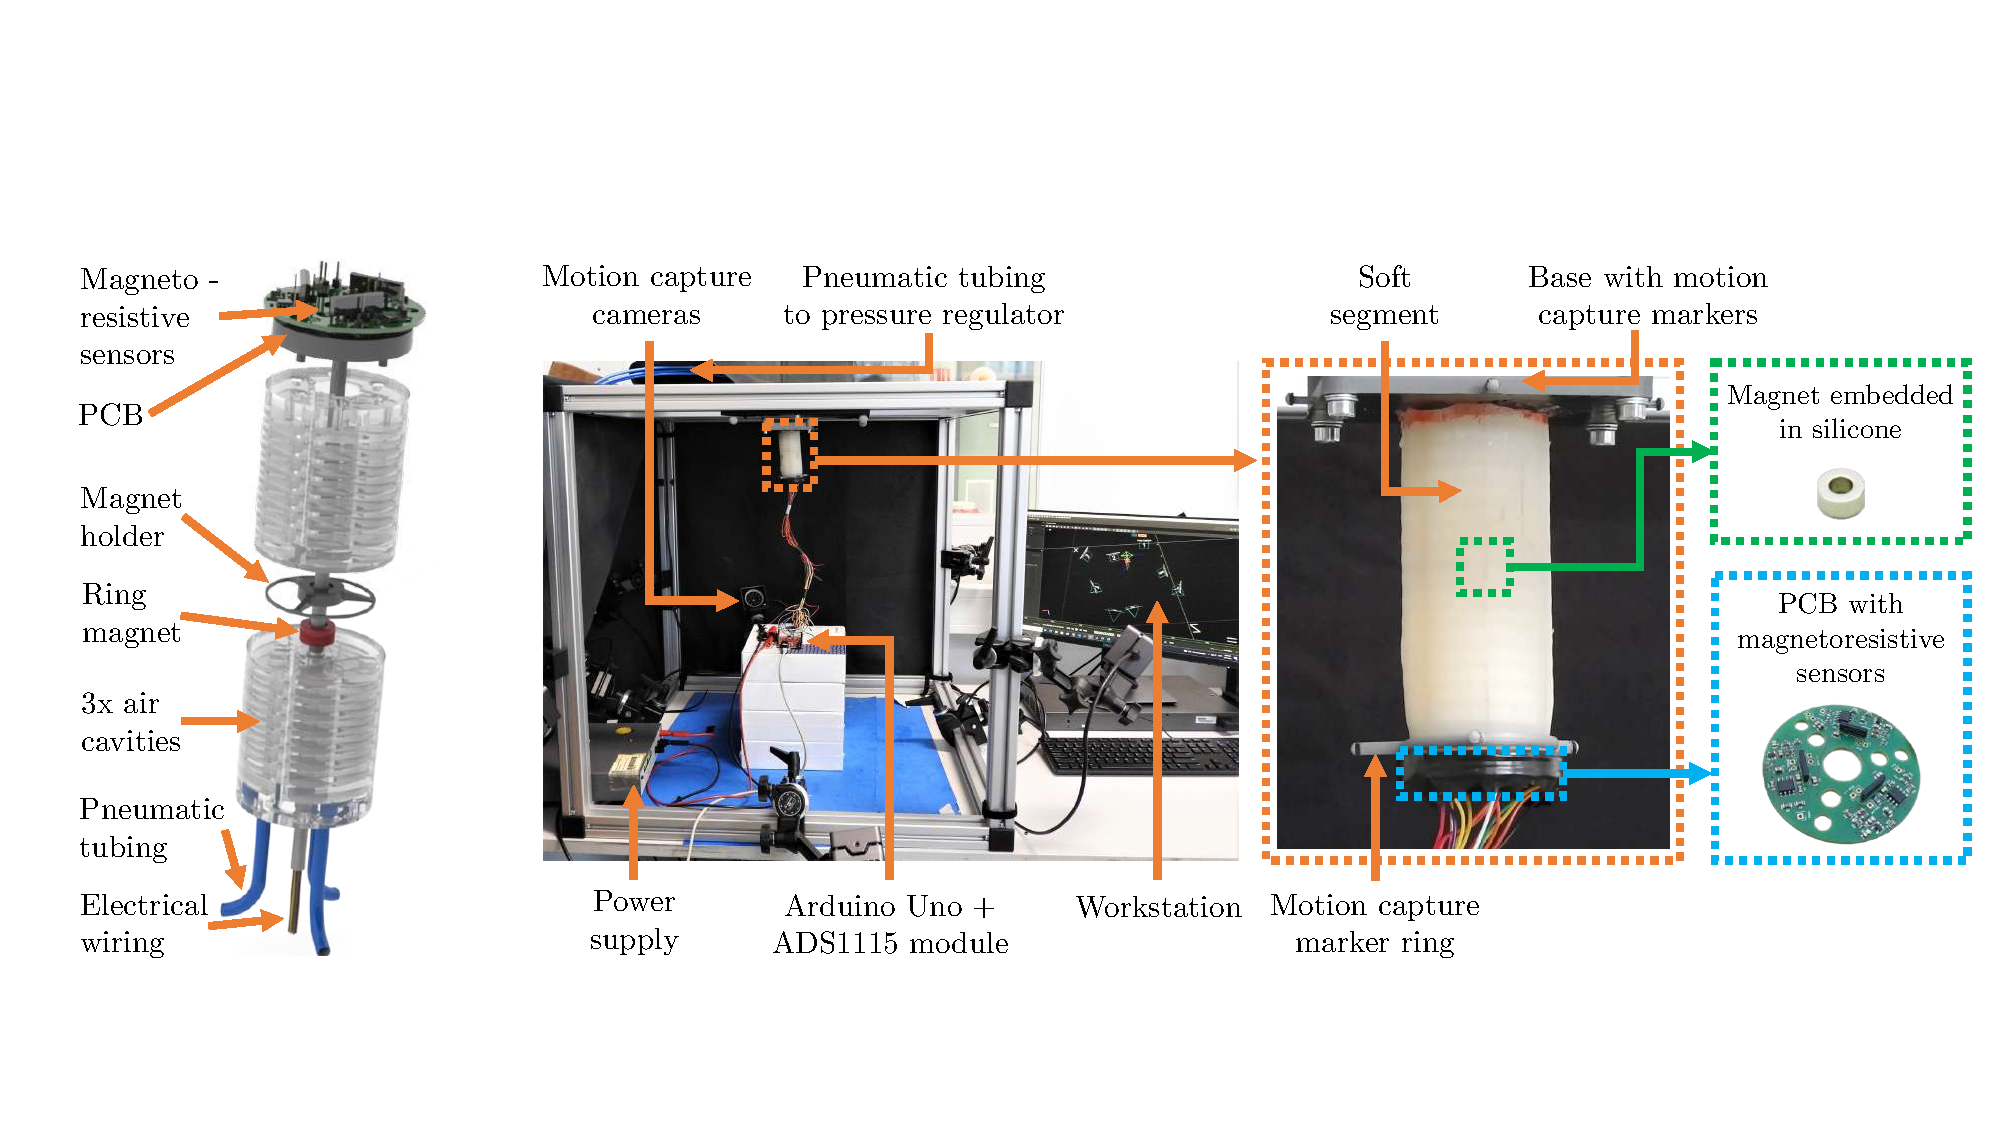
\includegraphics[width=1.0\textwidth]{promasens/figures/experimental_setup/experimental_setup_v5_compressed.pdf}
    \caption{
    \textbf{Left:} Exploded rendering visualizing the robot design with the three magnetoresistive sensors integrated into a PCB at the tip of the segment. The electrical wires from the PCB are passed through the backbone to the base. A ring magnet attached to a 3D-printed holder is integrated into the backbone at a half-segment-length distance from the proximal end. The air chambers of the segment are connected to a pressure regulator via tubing glued at the base of the segment. \textbf{Right:} Experimental setup with the soft robot segment attached in tip-down configuration to the motion capture cage.
    }\label{fig:promasens:experimental_setup}
\end{figure*}
% \begin{figure*}[hbt]
%     \centering
%     \subfigure[Design]{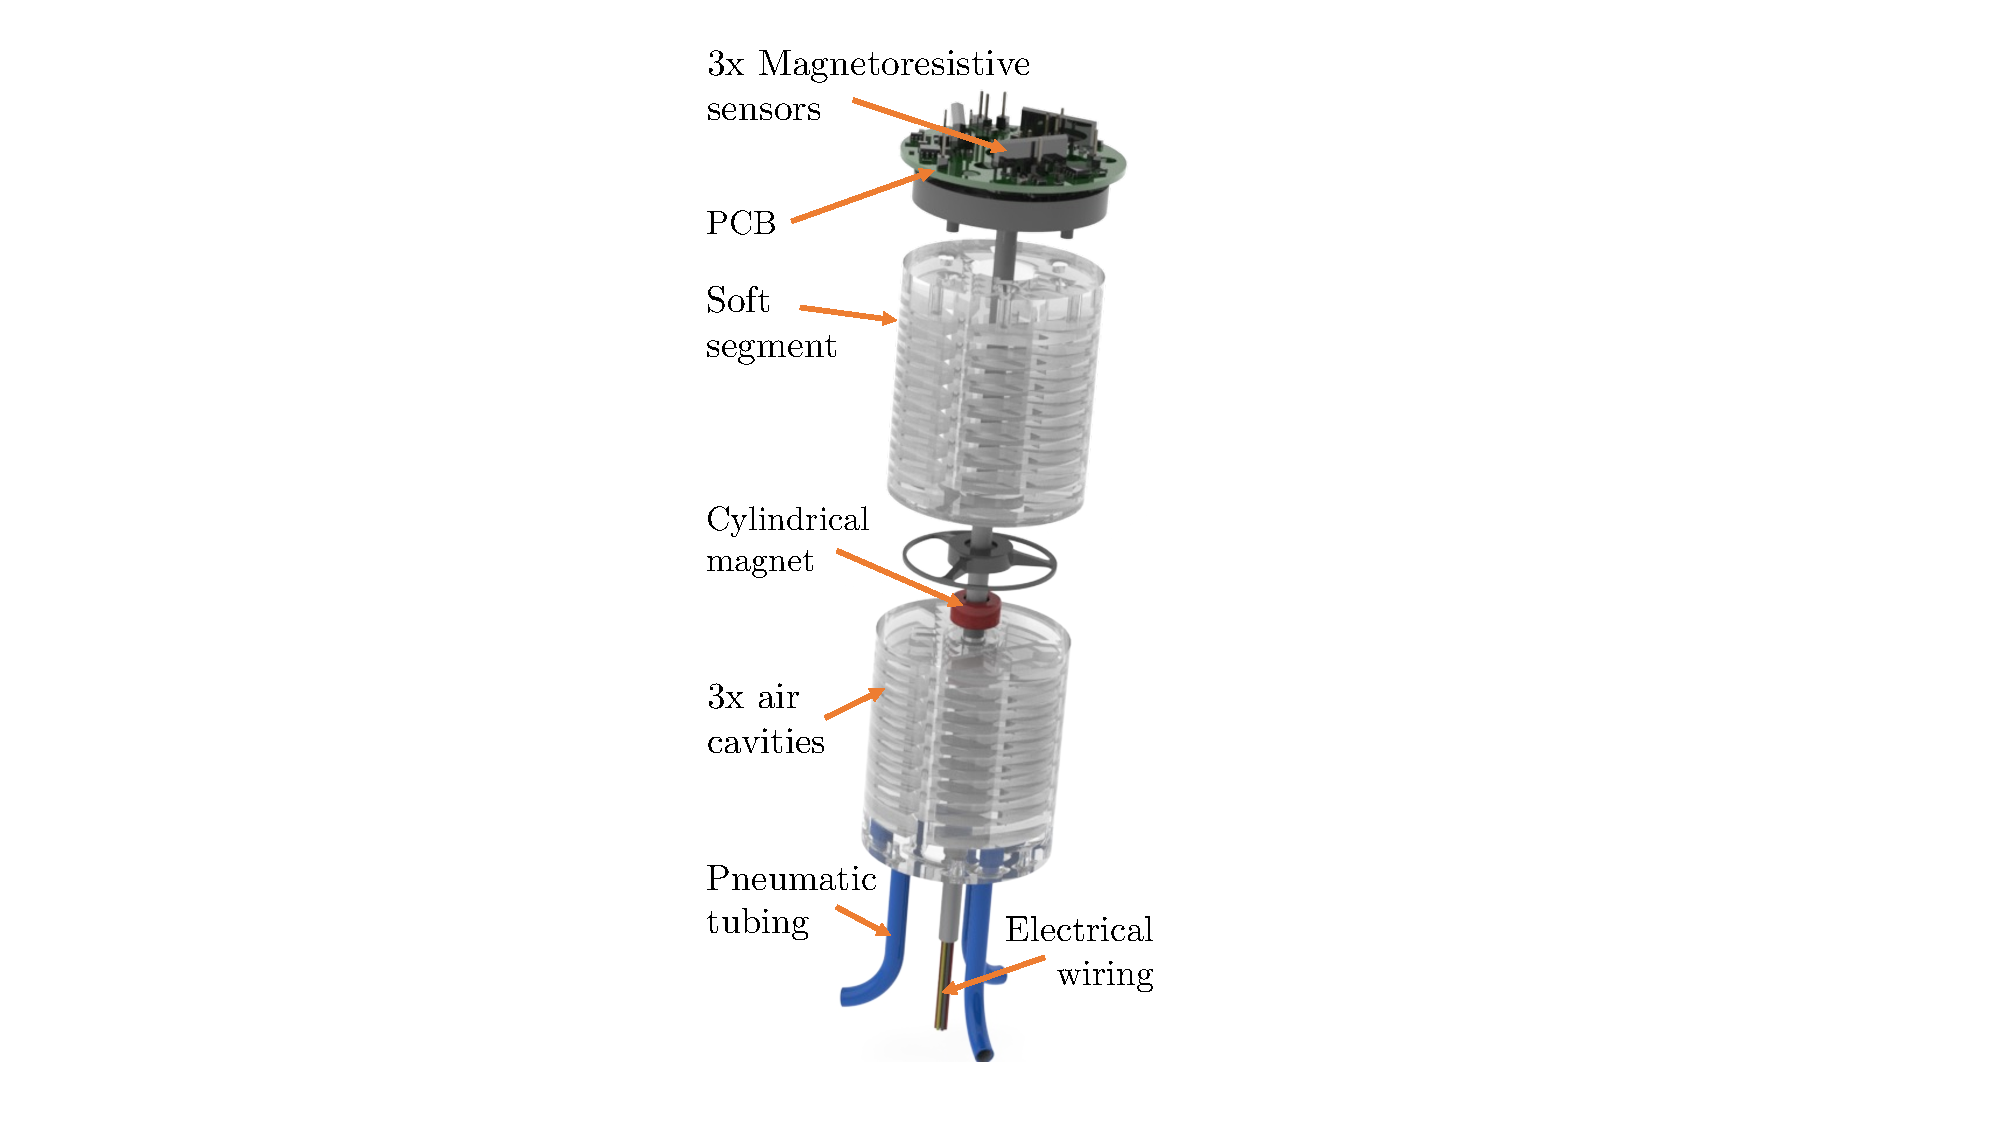
\includegraphics[width=0.135\textwidth]{promasens/figures/segment_design/segment_exploded_rendering_labeled_v1_cropped.pdf}\label{fig:promasens:exploded_rendering}}
    % \hspace{1pt}
%     \hfill
%     \subfigure[Experimental setup]{\includegraphics[width=0.65\textwidth]{promasens/figures/experimental_setup/experimental_setup_v4_compressed.pdf}\label{fig:promasens:experimental_setup}}
%     % \hspace{1pt}
%     \hfill
%     \subfigure[Actuated soft robot]{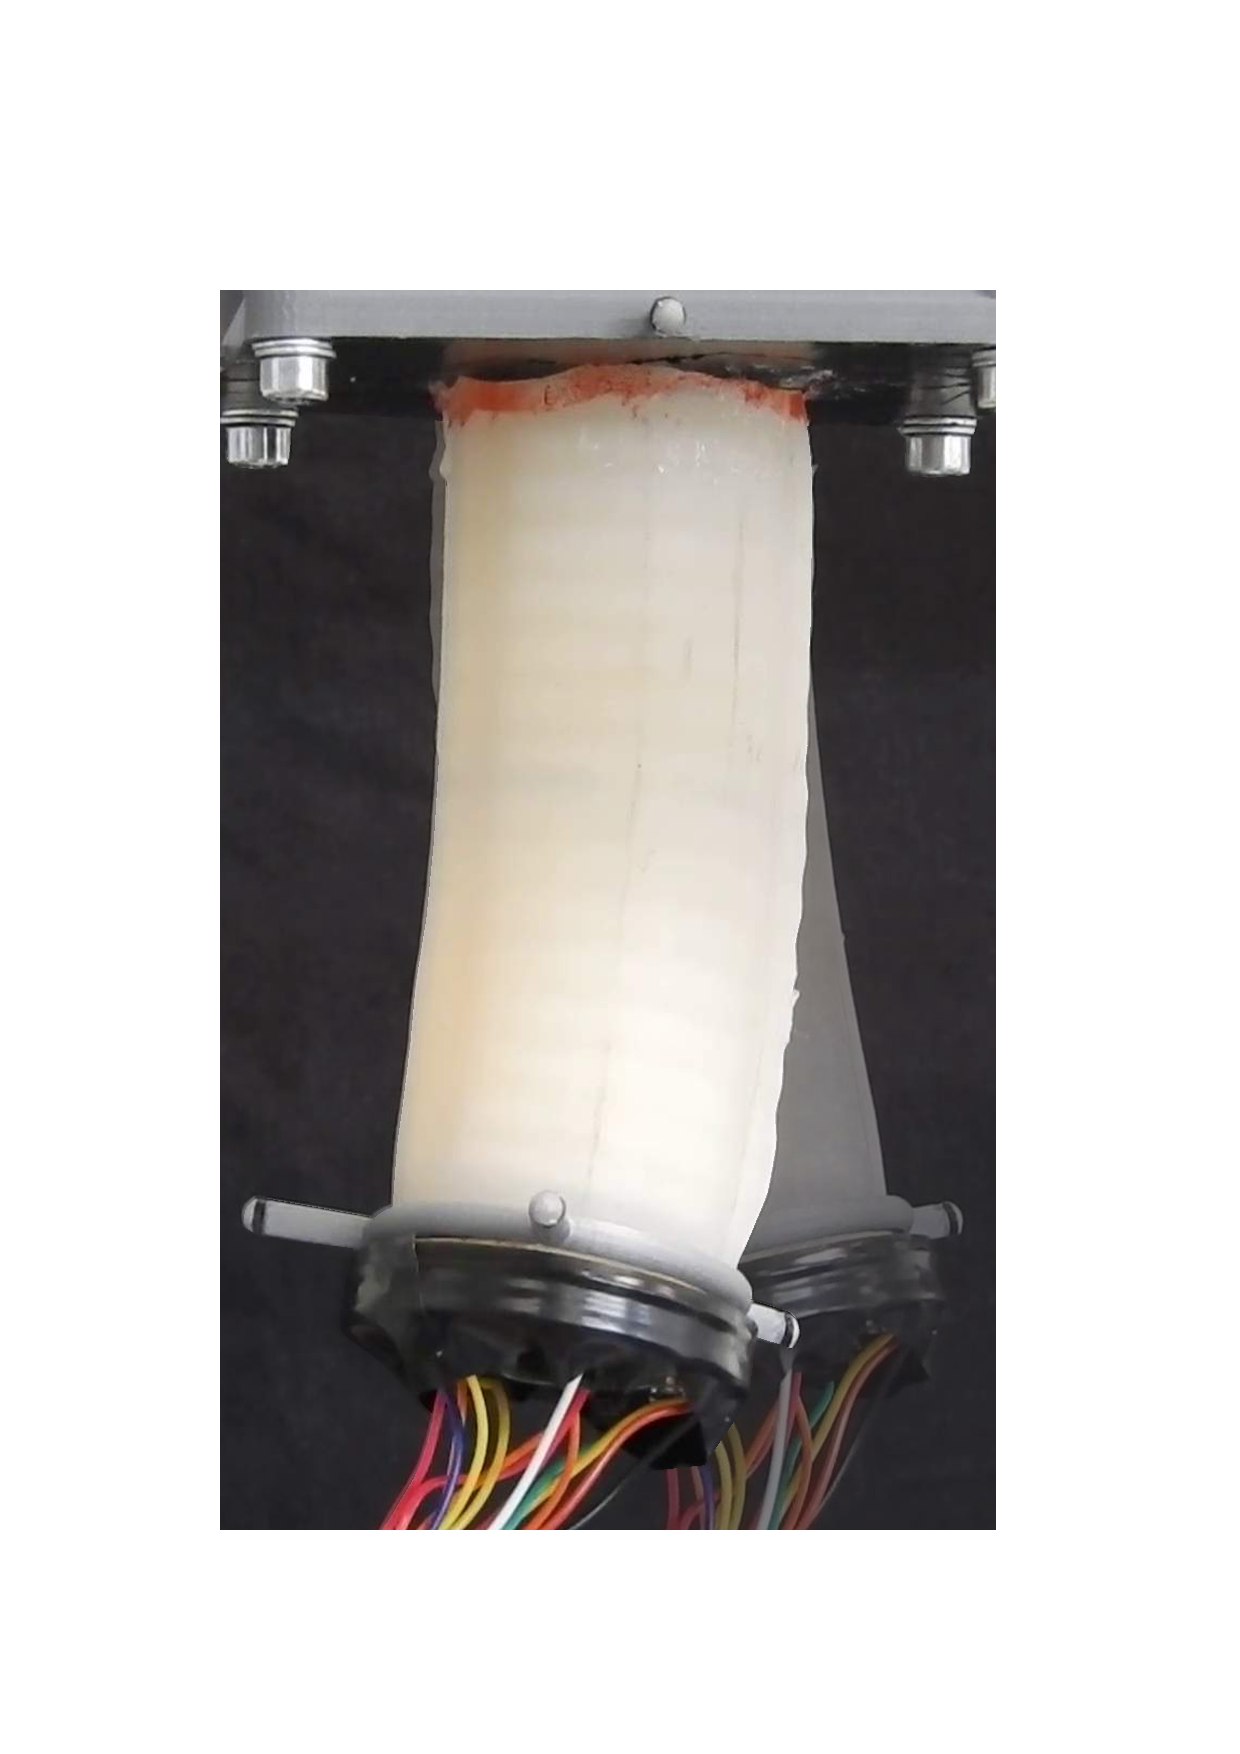
\includegraphics[width=0.16\textwidth]{promasens/figures/robot_bending/Overlapping_images_left_solid_right_transparent_compressed.pdf}\label{fig:promasens:actuated_soft_robot}}
%     \caption{\textbf{Panel (a):} Exploded rendering visualizing the robot design with the three magnetoresistive sensors integrated into a PCB at the tip of the segment. The electrical wires from the PCB are passed through the backbone to the base. A ring magnet attached to a 3D-printed holder is integrated into the backbone at a half-segment-length distance from the proximal end. The air chambers of the segment are connected to a pressure regulator via tubing glued at the base of the segment. \textbf{Panel (b):} Experimental setup with the soft robot segment attached in tip-down configuration to the motion capture cage. % Magnet and \gls{PCB} with \glsp{MRS} are scaled relative to the soft robot segment.
%     \textbf{Panel (c):} Evolution of a soft robot during 1D bending.}
% \end{figure*}

We verify the performance of our proposed proprioception method in experiments involving one soft robot segment with three magnetoresistive sensors attached to the tip.
We aim to estimate the CC configuration $\hat{q} = (\Delta_{x,1}, \Delta_{y,1})^\mathrm{T} \in \mathbb{R}^2$ from the measured sensor values $u(t) \in \mathbb{R}^3$.
% We collect a training set of random actuation sequences produced with \gls{GBN}~\cite{tulleken1990generalized}.
We let the robot follow a diverse set of trajectories and evaluate the proprioception performance.
After measuring the ground-truth pose of the tip of the segment with a motion capture system, we perform inverse kinematics with the closed-form solution reported by Della Santina et al.~\cite{della2020improved} and quantitatively compare the proprioceptive configuration estimate of the segment with the ground-truth configuration.

\begin{figure*}[hbt]
  \centering
  \subfigure[\textbf{T0:} random setpoints]{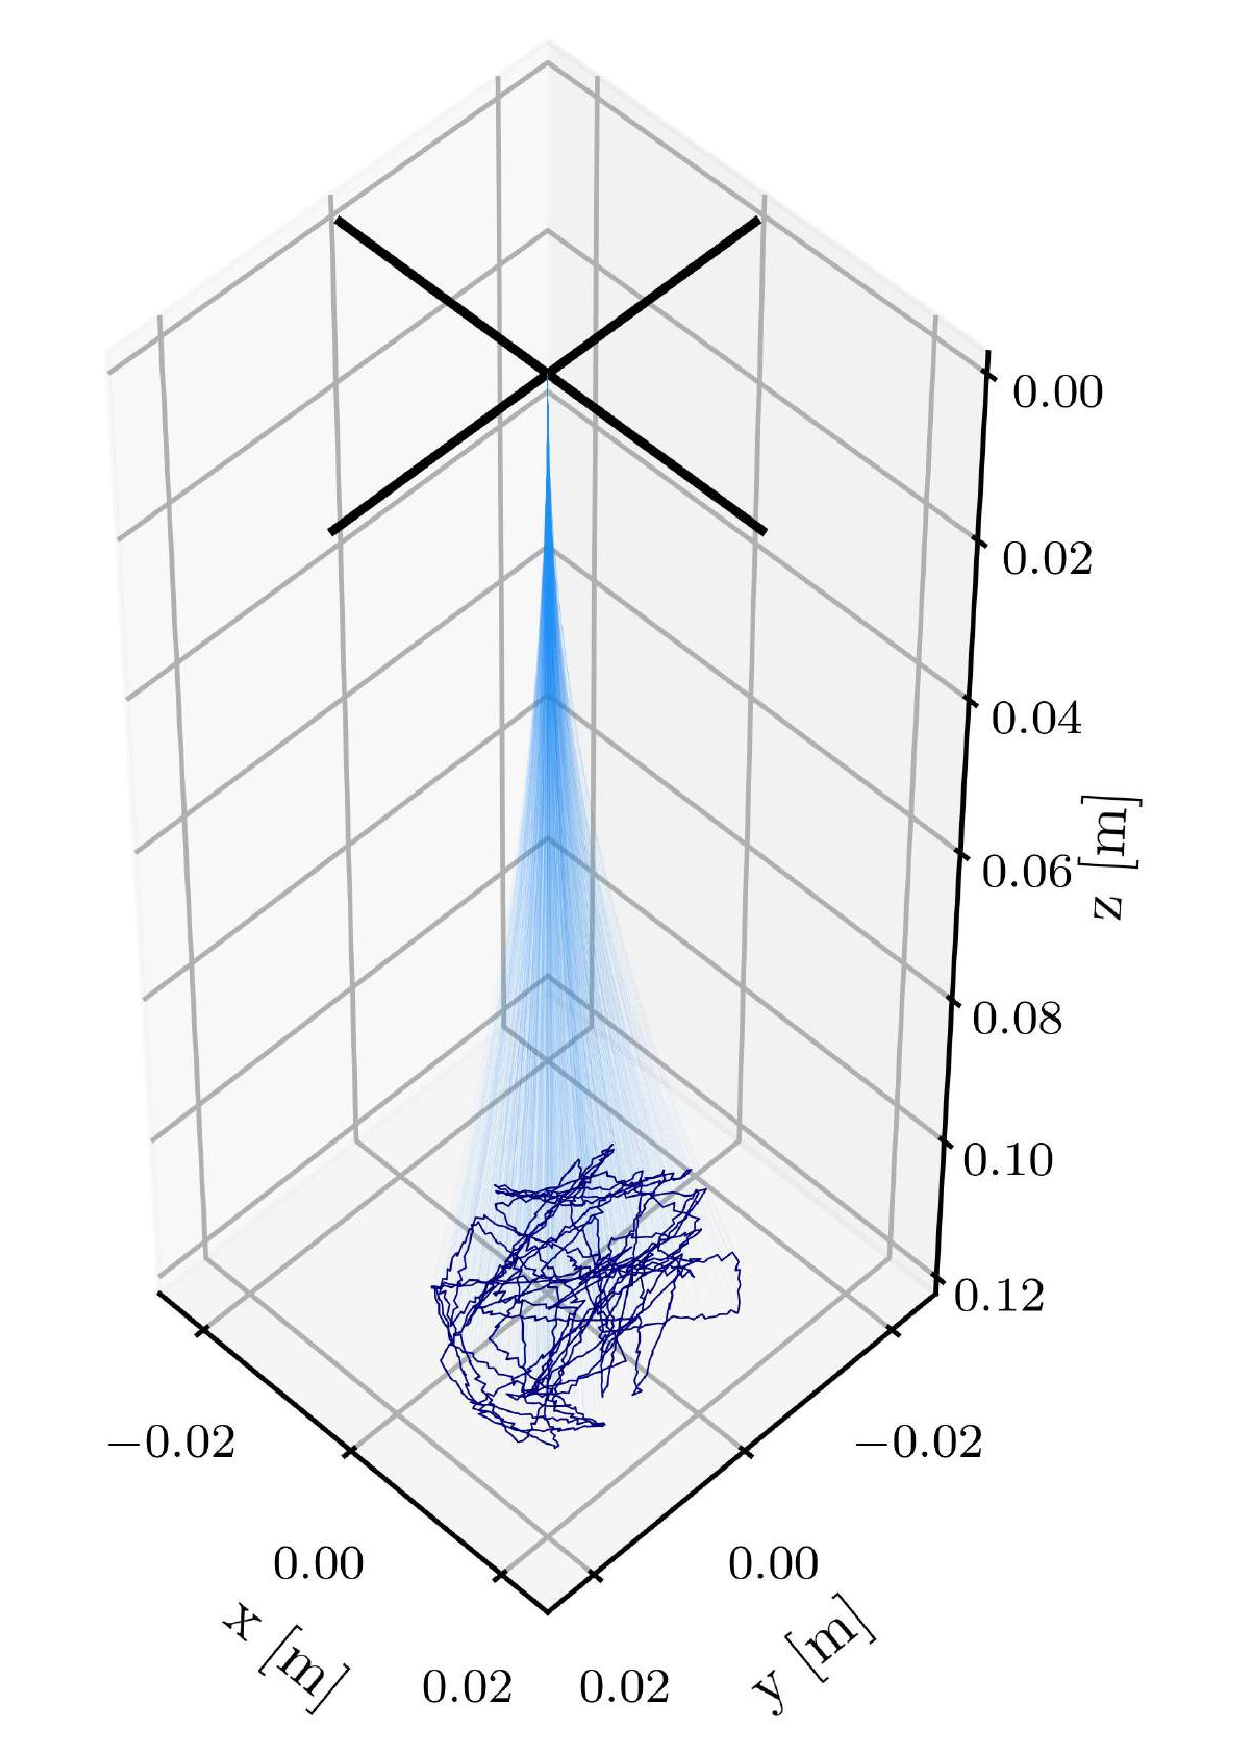
\includegraphics[width=0.16\textwidth]{promasens/figures/trajectories/trajectory_visualizations/random_compressed.pdf}}
  % \hfill% or \hspace{5mm} or \hspace{0.3\textwidth}
  \subfigure[\textbf{T1:} 1D bending]{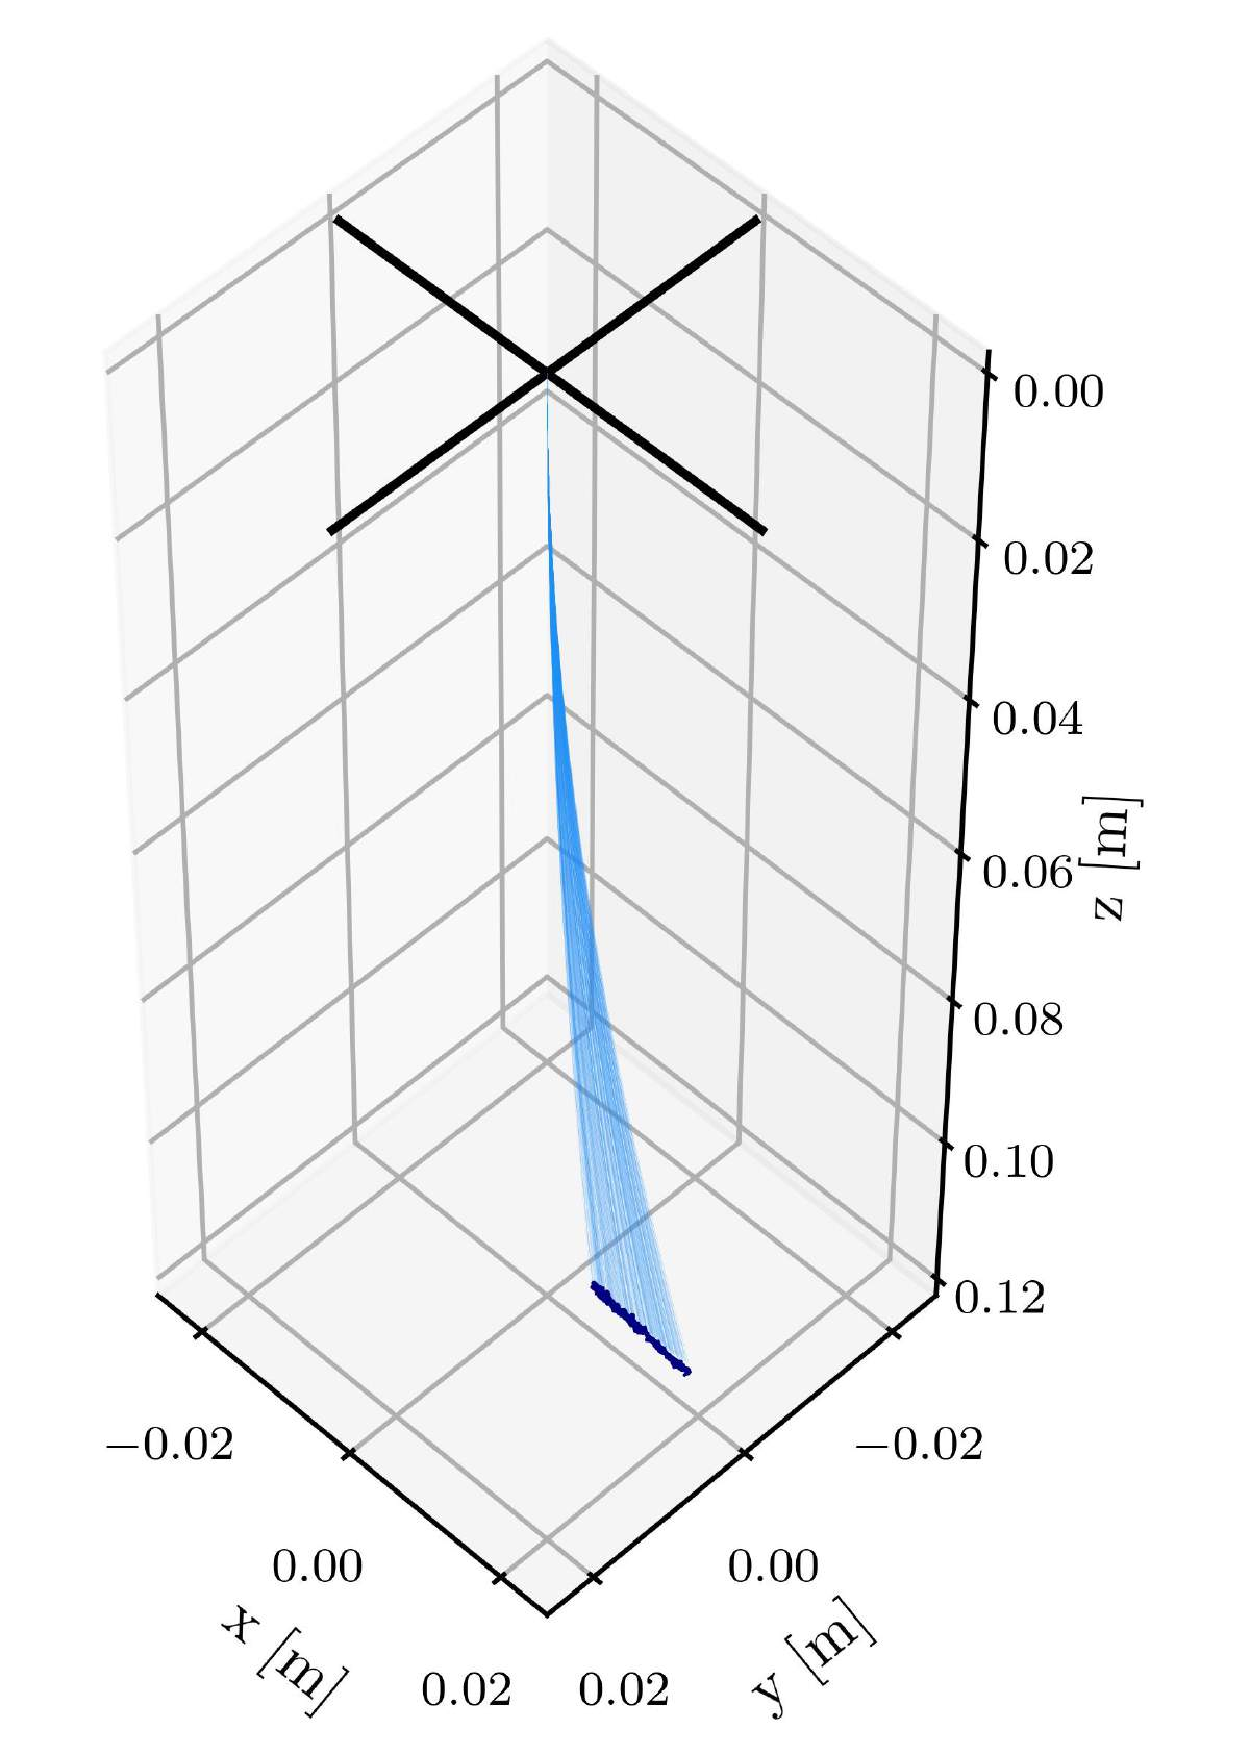
\includegraphics[width=0.16\textwidth]{promasens/figures/trajectories/trajectory_visualizations/1D_bending_compressed.pdf}}
  \subfigure[\textbf{T2:} half lemniscate]{\includegraphics[width=0.16\textwidth]{promasens/figures/trajectories/trajectory_visualizations/half_lemniscate_compressed.pdf}}
  \subfigure[\textbf{T3:} full lemniscate]{\includegraphics[width=0.16\textwidth]{promasens/figures/trajectories/trajectory_visualizations/full_lemniscate_compressed.pdf}\label{fig:promasens:t3_viz}}
  \subfigure[\textbf{T4:} spiral]{\includegraphics[width=0.16\textwidth]{promasens/figures/trajectories/trajectory_visualizations/spiral_compressed.pdf}}
  \subfigure[\textbf{T5:} flower]{\includegraphics[width=0.16\textwidth]{promasens/figures/trajectories/trajectory_visualizations/flower_compressed.pdf}}
%   \hfill
%   \subfigure[Neural network architecture]{\includegraphics[width=0.33\textwidth]{promasens/figures/Experiments/NN_architecture_P.pdf}\label{fig:promasens:NNgradientdescent}}
  \caption{Trajectories used during the experiments. We plot the shape of the segment under \gls{PCC} approximation in light blue and the position of the tip of the segment in dark blue. 
  % Trajectory 1 represents a 1D bending, trajectory 2 a half lemniscate, trajectory 3 a full lemniscate movement of the tip and trajectory 4 resembles a spiral. 
  % \textbf{Panel (e):} Architecture of the sensor measurement prediction network. Each block consists of a linear layer, a \gls{ReLU}, and a batch norm layer.
  }
  \label{fig:promasens:trajectories}
\end{figure*}

\subsection{Robot design}\label{sub:promasens:robot_design}
We use a cylindrical, pneumatically-actuated soft robotic silicon segment of length $L_{0}=\SI{110}{mm}$ and radius $d_1 = \SI{22}{mm}$ consisting of three independently inflatable cavities evenly spaced in the radial direction from the center line~\cite{marchese2015recipe}. 
% The robot is pneumatically actuated by adjusting the air pressure in each chamber to make the end-effector bend in 3D Cartesian space.
%
The proprioceptive sensing system is achieved by embedding one ring magnet in the backbone at a distance $d_{\mathrm{m}_0} = \SI{55}{mm}$ from the base of the segment and three symmetrically-placed Magnetoresistive Sensors (MRSs) at the tip of the segment as visualized in Fig.~\ref{fig:promasens:experimental_setup}. % Fig.~\ref{fig:promasens:exploded_rendering}.
Although we use MRSs in our experimental setup for their high sensitivity~\cite{popovic2002bridging}, this is not a strict condition and other sensor types measuring the magnetic field such as Hall-effect sensors can be combined with the methodology proposed in this chapter too.
For casting the silicone segment, we use a 3D-printed mold with a holder for the magnet which keeps it in place inside the segment.
The magnet used is a neodymium ring of grade N50 with a thickness and inner diameter of \SI{6}{mm} each, and an outer diameter of \SI{12}{mm}.
%
The MRSs of type Honeywell HMC1021Z are integrated into a Printed Circuit Board (PCB) and output a voltage difference of \SI{50}{mV \per mT}. % ~\cite{honeywell}. 
The three sensors are equally spaced at \SI{120}{\degree} from each other and are placed at a radial distance of $d_{\mathrm{s},\mathrm{r}} = \SI{13}{mm}$, and at a longitudinal distance of $d_{\mathrm{s},\mathrm{a}} = \SI{116}{mm}$ from the base in a straight configuration.
For each sensor, we implemented a Set / Reset and an amplification circuit on the PCB.
The Set / Reset circuit is used for calibration of the sensor by re-aligning the magnetic domains. After amplification of the sensor output by a factor of 100, the output of the sensors is processed with a Texas Instruments ADS1115 module %~\cite{ADS1115module}
resulting in a digital signal of \SI{16}{bit} resolution. All sensor measurements $u$ are in the range $[\SI{0}{mV}, \SI{2048}{mV}]$, which corresponds to magnetic flux densities of  $[\SI{0}{mT}, \SI{41}{mT}]$.

%The \gls{MRS} are mounted on a \gls{PCB} at the tip of the silicone body, with three sensors on one PCB. The exact placement of the sensors is shown in Table \ref{tab:sensor_locations}. The sensors are Honeywell HMC1021Z sensors that have an ideal operating range of $\SI{\pm 6}{Gs}$. The sensor gives a voltage difference of \SI{5}{mV \per Gs} as an output \cite{honeywell,farnell}.
%
% The \gls{PCB} is mounted on either side of the silicone body. The holes in the \gls{PCB} are for the air supply hoses, cables, and mounting. The \gls{PCB} not only contains the sensors, but also the sensor circuitry. Each sensor has its own circuitry containing a Set/Reset circuit and an amplification circuit. The Set/Reset circuit produces a current peak of \SI{1}{A} of duration $\SI{2}{\micro \second}$ for a Set/Reset pulse to calibrate the sensor by realigning the magnetic domains in the sensor in one direction. The amplification circuit amplifies the sensor output by a factor of 100. The output of the sensors is processed with a Texas Instruments ADS1115 module \cite{ADS1115module}. This module reads out the sensor signal in 16 bits and fits it into a format so that the Arduino can read it out. This gives a more precise sensor readout than using the Arduino directly which would only give a \SI{10}{bit} resolution.\\

% Fabrication
% The fabrication process of the silicone body starts by making three wax inserts by pouring beeswax into a silicone mold. Once hardened, these wax inserts are removed from their silicone mold and placed into a 3D-printed mold together with the magnet holder. The magnet holder is a 3D-printed ring that houses the magnet. Subsequently, Dragon Skin 30 silicone is mixed, degassed, and poured into the 3D-printed mold. After hardening, the silicone body, wherein the magnet holder and magnet are embedded, is removed from the mold. Then the wax inserts are melted, leaving three inflatable chambers behind.

% \begin{figure}[ht]
% \centering
% \includegraphics[width=50mm]{promasens/figures/PCB_3d_view_2.png}
% \caption{\gls{PCB} for three \gls{MRS} including Set/Reset circuit to be mounted at the base and tip of each segment.}\label{fig:promasens:PCB}
% \end{figure}
        

\begingroup
\setlength{\tabcolsep}{6pt} % Default value: 6pt
\begin{table*}\footnotesize
\centering
\caption{Experimental results: absolute [mm] and relative RMSE [\%] of sensor measurement predictions and robot configuration estimates for various trajectories. The RMSE is normalized with the range of the dataset for $u$ and each configuration variable respectively as stated in \eqref{eq:promasens:relative_RMSE}. We report the error as $\text{mean} \pm \text{stdev}$ and compute the statistics over three different random seeds. The random seed determines at the start of the training the initialization of the neural network weights.}
\begin{tabular}{l rr rrrr}\toprule
\textbf{Trajectory} & $e_{u}$ [mV] & $e_{u}$ [\%] & $e_{\Delta_x}$ [mm] & $e_{\Delta_x}$ [\%] & $e_{\Delta_y}$ [mm] & $e_{\Delta_y}$ [\%]\\
\midrule
T5.train $\rightarrow$ T0.test & $9.90 \pm 0.90$ & $3.90 \pm 0.40$ & $0.37 \pm 0.06$ & $3.70 \pm 0.60$ & $0.44 \pm 0.01$ & $3.50 \pm 0.10$\\ % T5.slow_to_T0.200mBar
T5.train $\rightarrow$ T1.test & $8.80 \pm 0.30$ & $4.40 \pm 0.10$ & $0.36 \pm 0.08$ & $6.50 \pm 1.50$ & $0.43 \pm 0.05$ & -\\ % T5.slow_to_T1.270
T5.train $\rightarrow$ T2.test & $11.10 \pm 0.30$ & $4.30 \pm 0.10$ & $0.78 \pm 0.03$ & $13.60 \pm 0.60$ & $0.74 \pm 0.23$ & $5.90 \pm 1.80$\\ % T5.slow_to_T2
T5.train $\rightarrow$ T3.test & $12.30 \pm 0.30$ & $4.60 \pm 0.10$ & $0.52 \pm 0.06$ & $4.50 \pm 0.50$ & $0.47 \pm 0.03$ & $3.10 \pm 0.20$\\ % T5.slow_to_T3_90deg
T5.train $\rightarrow$ T4 & $3.01 \pm 0.05$ & $1.08 \pm 0.02$ & $0.33 \pm 0.02$ & $2.40 \pm 0.10$ & $0.52 \pm 0.06$ & $3.10 \pm 0.40$\\ % T5.slow_to_T4.slow.forw
T5.train $\rightarrow$ T5.test & $1.60 \pm 0.10$ & $0.58 \pm 0.05$ & $0.24 \pm 0.05$ & $1.90 \pm 0.30$ & $0.24 \pm 0.01$ & $1.40 \pm 0.05$\\ % T5.slow_to_T5.slow
\bottomrule
\end{tabular}
\label{tab:results_experiments}
\end{table*}
\endgroup

\subsection{Experimental setup}
We conducted our experiments in a lab environment with the base of the soft robot segment mounted in a tip-down configuration to a cubical cage as shown in Figure~\ref{fig:promasens:experimental_setup}.
% Motion Capture System
A 3D-printed ring with four reflective markers is mounted on the tip of the segment.
% Prime X by Optitrack
Eight motion capture cameras are attached to the cage tracking at \SI{40}{Hz} the 3D pose of the ring.
We transform the pose measurements of the tip to the base frame of the robot and compute the closed-form inverse kinematics~\cite{della2020improved} to receive a ground-truth configuration estimate $q(t) \in \mathbb{R}^2$.
% Pneumatic actuation
Each of the three pneumatic chambers of the segment is connected via tubing to a separate valve of a proportional pressure regulator operated at \SI{100}{Hz}. % We send set-point pressure commands from the workstation to the pressure regulator via Modbus / TCP at \SI{100}{Hz}.
% Reading sensor measurements
We read out the analog signals of the magnetoresistive sensors with an Arduino Uno at \SI{40}{Hz} and save them for later offline processing. 
We temporally align the motion capture and the magnetic sensor data by detecting the initial extension of the robot with a suitable threshold.
%static distortion
The sensor noise is determined for both an unelongated straight configuration, and during fully inflated bending. Here the standard deviations of the white noise are \SI{0.24}{mV} and \SI{3.55}{mV}, which normalizes to \SI{0.03}{\percent} and \SI{2}{\percent} of the dynamic range respectively.
% earth's magnetic field
% Furthermore, we measure the angle between the x-axis of the base frame and the magnetic north with a compass as $\varphi_\mathrm{e} = \SI{3.79}{\radian}$ and rely on the \gls{WMM}~\cite{chulliat2020us} to identify the vertical component of the earth's magnetic field. This results in a unit vector for the earth's magnetic field direction of $\{ \hat{n}_{\mathrm{e}} \}_{0} = (-0.311, -0.234, 0.921)^\mathrm{T}$ for the robot in tip-down configuration.
Furthermore, we identify the earth's magnetic field direction in the base from as $\{ \hat{n}_{\mathrm{e}} \}_{0} = (-0.311, -0.234, 0.921)^\mathrm{T}$ using a compass and the World Magnetic Model (WMM)~\cite{chulliat2020us}.

\begin{figure*}[hbt]
  \centering
  \subfigure[Loss landscape]{\includegraphics[width=0.3125\textwidth]{promasens/figures/loss_landscape/loss_landscape_v3_cropped.pdf}\label{fig:promasens:loss_landscape}}
  %
  \subfigure[Experimental results for T2 (top) and T5 (bottom)]{\includegraphics[width=0.6775\textwidth]{promasens/figures/experimental_results/2022-05-02_results_merged.pdf}\label{fig:promasens:2022-05-02_results_merged}}\\ %  [T5.train $\rightarrow$ T2.test] [T5.train $\rightarrow$ T5.test]
  
  \caption{\textbf{Panel (a):} Sample loss landscape for optimization of $\Delta_x$ and $\Delta_y$ on T5. With the hue, we visualize the RMSE of the sensor measurement prediction $\hat{u}$ for a given configuration $\hat{q} = (\Delta_x, \Delta_y)^\mathrm{T}$. Additionally, we denote the initial configuration estimate with $\hat{q}_0$, the trajectory of the gradient descent with $\hat{q}_l$, the optimal configuration with $\hat{q}$, and the ground truth with $q$. \textbf{Panel (b) top:} Proprioception on the test set of T2 using a model trained on T5. \textbf{Panel (b) bottom:} Configuration estimates for a model trained and evaluated on separated parts of trajectory 5. We plot the ground-truth configuration $q$ in solid, the estimate $\hat{q}$ as a mean over three random seeds with dashed lines, and the standard deviation as an error band. The bottom right plot zooms onto a selected part of T5 (e.g. \SI{18}{s} to \SI{22}{s}) to more clearly visually distinguish the dashed lines from the solid lines.}
  \label{fig:promasens:results_trajectories}
\end{figure*}

\subsection{Pneumatic actuation and trajectories}
% We consider two actuation sequence types in this chapter: a) a randomized actuation sequence consisting of steps generated with \gls{GBN}~\cite{tulleken1990generalized} primarily used for training and b) three continuous trajectories consisting of planar side bending, and the tip following half-8-shape and full 8-shapes as plotted in Fig.~\ref{fig:promasens:trajectories}.
We consider, as visualized in Fig.~\ref{fig:promasens:trajectories}, six continuous actuation sequences in this chapter: random configuration way-points which are connected through linear interpolation (T0), planar side bending (T1), the tip following a half lemniscate (T2) and full lemniscate (T3), a spiral with constant linear velocity~\cite{carrasco2018constant} (T4) and finally a flower-shape (T5).
We define our trajectories as wrenches  $\tau_\mathrm{xyz} = \begin{bmatrix} \tau_\mathrm{x} & \tau_\mathrm{y} \end{bmatrix}^\mathrm{T}$ on the tip of the segment in Cartesian space, where $\tau_\mathrm{x}$ and $\tau_\mathrm{y}$ cause bending around the local x- and y-axis  of the tip respectively. % $f_\mathrm{z}$ is a force leading the segment to extend uniformly.
The pressures we command from the pressure regulator are given by inversely evaluating the force produced at the center of pressure at the tip of the segment for each chamber for a given chamber pressure~\cite{della2019dynamic}.
All actuation sequences are preceded by first applying an offset pressure of \SI{225}{mBar} in all chambers, which causes a near-constant elongation of the segment. The peak pressure, which causes maximum bending, is set for all trajectories to \SI{450}{mBar}.

% The \gls{GBN}~\cite{tulleken1990generalized} algorithm with an expected settling time of \SI{5}{s} determines the timing of when we command a step to a new random wrench $\tau_{xzy}$.
% We uniformly sample a bending azimuth angle $\varphi \sim \mathcal{U}\left(0, 2 \pi\right)$, a bending torque magnitude $|\tau| \sim \mathcal{U}\left(0, \tau_\mathrm{max}\right)$ and accordingly compute $\tau_\mathrm{xyz}$ as
% \begin{equation}
%     \tau_\mathrm{x} = \cos(\varphi) |\tau| \qquad \tau_\mathrm{y} = \sin(\varphi) |\tau|
% \end{equation}
% and set $f_\mathrm{z}$ to a constant force with corresponding symmetric pressure of \SI{200}{mBar} in the chambers. The maximum bending torque $\tau_\mathrm{max}$ corresponds to a peak pressure in the chambers of \SI{425}{mBar}

% The planar side bending, half lemniscate, and full lemniscate trajectories are generated with a recurring linear torque increase/decrease sequence up to a peak pressure of \SI{425}{mBar}.
% Each T1-T3 trajectory is repeated six times to extend the length of the dataset.
% The spiral trajectory consists of linearly increasing the torque amplitude from a peak pressure of \SI{305}{mBar} to \SI{425}{mBar} over a duration of \SI{110}{s} while at the same time tracking a circular motion with an angular velocity of \SI{1.26}{rad/s}. In the second half of the trajectory, which is later used as a test set, the peak pressure is accordingly linearly decreased over time.

%The spiral trajectory consists of linearly increasing the torque amplitude from a peak pressure of \SI{305}{mBar} to \SI{425}{mBar} over a duration of \SI{110}{s} while at the same time tracking a circular motion with an angular velocity of \SI{1.26}{rad/s}. In the second half of the trajectory, which is later used as a test set, the peak pressure is accordingly linearly decreased over time. 

%The first part is generated with
%\begin{equation}
%    \tau_\mathrm{x} = \frac{2 t}{n_\mathrm{t}} \sin(2 \pi f t) \,     \tau_\mathrm{max} \qquad \tau_\mathrm{y} = \frac{2        t}{n_\mathrm{t}} \sin(2 \pi f t) \, \tau_\mathrm{max},
%\end{equation}
%where $f=\SI{0.2}{Hz}$ represents the frequency, and $\tau_\mathrm{max}$ the peak bending torque of the trajectory with a corresponding peak pressure of \SI{410}{mBar} in the chambers. We denote with $t$ the time and $n_\mathrm{t}$ the duration of the trajectory.

%Very similarly, we generate the planar side bending, half-8-shape, and full-8-shape trajectories with a recurring linear torque increase/decrease sequence up to a peak pressure of \SI{410}{mBar}.
%Each T1-T3 trajectory is repeated six times to extend the length of the dataset.

% We generate the planar side bending, half-8-shape, and full 8-shape trajectories with the following function:
% \begin{equation}
%     \tau_\mathrm{x} = A_x \sin(2 \pi F_x f t) \tau_\mathrm{max} \qquad \tau_\mathrm{y} = A_y \sin(2 \pi F_y f t) \tau_\mathrm{max}
% \end{equation}
% with an offset pressure of \SI{200}{mBar} causing a constant extension of the segment, $f$ representing the trajectory frequency, $\tau_\mathrm{max}$ the peak bending torque of the trajectory with a corresponding peak pressure of \SI{410}{mBar} in the chambers and $t$ the trajectory time.
% Duration of $n_\mathrm{t}=\SI{3.8}{s}$
% \textcolor{red}{TODO: fix this}
% We choose $F_x$, $F_y$, $A_x$, and $A_y$ appropriately to generate the different trajectories, which we report in Tab.~\ref{tab:trajectory_params}.

The 1D bending (T1), half lemniscate (T2) and full lemniscate (T3) are all executed periodically with a period of \SI{5}{s}, \SI{10}{s}, and \SI{10}{s} respectively. 
Trajectories T0 and T4 are characterized by a constant velocity in torque-space of \SI{0.025}{Nm \per s} and \SI{0.0125}{kNm \per s} respectively.
The flower trajectory T5 can be described as periodic 1D bending with a linearly changing azimuth angle. It exhibits an angular velocity of \SI{0.0126}{rad \per s} and a period of \SI{10}{s} for the bending, which results in $50$ bending cycles per circumnavigation.
While the random configuration setpoints of T0 are recorded for \SI{200}{s}, T1, T2 and T3 have total a duration of \SI{90}{s} each, and the spiral T4 and flower T5 last for \SI{120}{s} and \SI{1500}{s} respectively.
We split off the final \SI{20}{\percent} of all datasets as a test set.


% \begin{figure*}[ht]
%     \centering
%     \scalebox{0.5}{
%     \begin{tabular}{llllllllll}
%     \includegraphics[width=0.15\linewidth]{promasens/figures/Experiments/T1F/T1Fscene00001.png} &
%     \includegraphics[width=0.15\linewidth]{promasens/figures/Experiments/T1F/T1Fscene00031.png} &
%     \includegraphics[width=0.15\linewidth]{promasens/figures/Experiments/T1F/T1Fscene00061.png} &
%     \includegraphics[width=0.15\linewidth]{promasens/figures/Experiments/T1F/T1Fscene00091.png} &
%     \includegraphics[width=0.15\linewidth]{promasens/figures/Experiments/T1F/T1Fscene00121.png} &
%     \includegraphics[width=0.15\linewidth]{promasens/figures/Experiments/T1F/T1Fscene00151.png} &
%     \includegraphics[width=0.15\linewidth]{promasens/figures/Experiments/T1F/T1Fscene00181.png} &
%     \includegraphics[width=0.15\linewidth]{promasens/figures/Experiments/T1F/T1Fscene00211.png} &
%     \includegraphics[width=0.15\linewidth]{promasens/figures/Experiments/T1F/T1Fscene00301.png} &
%     \includegraphics[width=0.15\linewidth]{promasens/figures/Experiments/T1F/T1Fscene00331.png} \\
%     \includegraphics[width=0.15\linewidth]{promasens/figures/Experiments/T1S/T1Sscene00001.png} &
%     \includegraphics[width=0.15\linewidth]{promasens/figures/Experiments/T1S/T1Sscene00031.png} &
%     \includegraphics[width=0.15\linewidth]{promasens/figures/Experiments/T1S/T1Sscene00061.png} &
%     \includegraphics[width=0.15\linewidth]{promasens/figures/Experiments/T1S/T1Sscene00091.png} &
%     \includegraphics[width=0.15\linewidth]{promasens/figures/Experiments/T1S/T1Sscene00121.png} &
%     \includegraphics[width=0.15\linewidth]{promasens/figures/Experiments/T1S/T1Sscene00151.png} &
%     \includegraphics[width=0.15\linewidth]{promasens/figures/Experiments/T1S/T1Sscene00181.png} &
%     \includegraphics[width=0.15\linewidth]{promasens/figures/Experiments/T1S/T1Sscene00211.png} &
%     \includegraphics[width=0.15\linewidth]{promasens/figures/Experiments/T1S/T1Sscene00301.png} &
%     \includegraphics[width=0.15\linewidth]{promasens/figures/Experiments/T1S/T1Sscene00331.png}
%  \\
%     \end{tabular}}
%     \caption{Trajectory 1: sequence of stills from a front view (top row) and side view (bottom row)}
%     \label{fig:promasens:trajectory_snapshots_T1}
% \end{figure*}

% \begin{figure*}[ht]
%     \centering
%     \scalebox{0.5}{
%     \begin{tabular}{llllllllll}
%     \includegraphics[width=0.15\linewidth]{promasens/figures/Experiments/T2F/T2Fscene00059.png} &
%     \includegraphics[width=0.15\linewidth]{promasens/figures/Experiments/T2F/T2Fscene00088.png} &
%     \includegraphics[width=0.15\linewidth]{promasens/figures/Experiments/T2F/T2Fscene00117.png} &
%     \includegraphics[width=0.15\linewidth]{promasens/figures/Experiments/T2F/T2Fscene00146.png} &
%     \includegraphics[width=0.15\linewidth]{promasens/figures/Experiments/T2F/T2Fscene00175.png} &
%     \includegraphics[width=0.15\linewidth]{promasens/figures/Experiments/T2F/T2Fscene00204.png} &
%     \includegraphics[width=0.15\linewidth]{promasens/figures/Experiments/T2F/T2Fscene00233.png} &
%     \includegraphics[width=0.15\linewidth]{promasens/figures/Experiments/T2F/T2Fscene00262.png} &
%     \includegraphics[width=0.15\linewidth]{promasens/figures/Experiments/T2F/T2Fscene00291.png} &
%     \includegraphics[width=0.15\linewidth]{promasens/figures/Experiments/T2F/T2Fscene00320.png} \\
%     \includegraphics[width=0.15\linewidth]{promasens/figures/Experiments/T2S/T2Sscene00061.png} &
%     \includegraphics[width=0.15\linewidth]{promasens/figures/Experiments/T2S/T2Sscene00061.png} &
%     \includegraphics[width=0.15\linewidth]{promasens/figures/Experiments/T2S/T2Sscene00091.png} &
%     \includegraphics[width=0.15\linewidth]{promasens/figures/Experiments/T2S/T2Sscene00121.png} &
%     \includegraphics[width=0.15\linewidth]{promasens/figures/Experiments/T2S/T2Sscene00151.png} &
%     \includegraphics[width=0.15\linewidth]{promasens/figures/Experiments/T2S/T2Sscene00181.png} &
%     \includegraphics[width=0.15\linewidth]{promasens/figures/Experiments/T2S/T2Sscene00211.png} &
%     \includegraphics[width=0.15\linewidth]{promasens/figures/Experiments/T2S/T2Sscene00241.png} &
%     \includegraphics[width=0.15\linewidth]{promasens/figures/Experiments/T2S/T2Sscene00271.png} &
%     \includegraphics[width=0.15\linewidth]{promasens/figures/Experiments/T2S/T2Sscene00301.png} \\
%  \\
%     \end{tabular}}
%     \caption{Trajectory 2: sequence of stills from a front view (top row) and side view (bottom row)}
%     \label{fig:promasens:trajectory_snapshots_T2}
% \end{figure*}

% \begin{figure*}[ht]
%     \centering
%     \scalebox{0.5}{
%     \begin{tabular}{llllllllll}
%     \includegraphics[width=0.15\linewidth]{promasens/figures/Experiments/T3F/T3Fscene00121.png} &
%     \includegraphics[width=0.15\linewidth]{promasens/figures/Experiments/T3F/T3Fscene00151.png} &
%     \includegraphics[width=0.15\linewidth]{promasens/figures/Experiments/T3F/T3Fscene00181.png} &
%     \includegraphics[width=0.15\linewidth]{promasens/figures/Experiments/T3F/T3Fscene00211.png} &
%     \includegraphics[width=0.15\linewidth]{promasens/figures/Experiments/T3F/T3Fscene00241.png} &
%     \includegraphics[width=0.15\linewidth]{promasens/figures/Experiments/T3F/T3Fscene00271.png} &
%     \includegraphics[width=0.15\linewidth]{promasens/figures/Experiments/T3F/T3Fscene00301.png} &
%     \includegraphics[width=0.15\linewidth]{promasens/figures/Experiments/T3F/T3Fscene00331.png} &
%     \includegraphics[width=0.15\linewidth]{promasens/figures/Experiments/T3F/T3Fscene00361.png} &
%     \includegraphics[width=0.15\linewidth]{promasens/figures/Experiments/T3F/T3Fscene00391.png} \\
%     \includegraphics[width=0.15\linewidth]{promasens/figures/Experiments/T3S/T3Sscene00121.png} &
%     \includegraphics[width=0.15\linewidth]{promasens/figures/Experiments/T3S/T3Sscene00151.png} &
%     \includegraphics[width=0.15\linewidth]{promasens/figures/Experiments/T3S/T3Sscene00181.png} &
%     \includegraphics[width=0.15\linewidth]{promasens/figures/Experiments/T3S/T3Sscene00211.png} &
%     \includegraphics[width=0.15\linewidth]{promasens/figures/Experiments/T3S/T3Sscene00241.png} &
%     \includegraphics[width=0.15\linewidth]{promasens/figures/Experiments/T3S/T3Sscene00271.png} &
%     \includegraphics[width=0.15\linewidth]{promasens/figures/Experiments/T3S/T3Sscene00301.png} &
%     \includegraphics[width=0.15\linewidth]{promasens/figures/Experiments/T3S/T3Sscene00331.png} &
%     \includegraphics[width=0.15\linewidth]{promasens/figures/Experiments/T3S/T3Sscene00361.png} &
%     \includegraphics[width=0.15\linewidth]{promasens/figures/Experiments/T3S/T3Sscene00391.png} \\
%     \end{tabular}}
%     \caption{Trajectory 3: sequence of stills from a front view (top row) and side view (bottom row)}
%     \label{fig:promasens:trajectory_snapshots_T3}
% \end{figure*}

% \begingroup
% \setlength{\tabcolsep}{3.5pt} % Default value: 6pt
% \begin{table*}% 
% \centering
% \caption{Experimental results: absolute and relative \gls{RMSE} of sensor measurement predictions by the neural network. For the relative RMSE, the absolute RMSE is normalized with the range of $u$ on the test set. We report the error as $\text{mean} \pm \text{stdev}$ and compute the statistics over three different random seeds.}
% \begin{tabular}{l cc cc cc}\toprule
% \textbf{Error} & \textbf{T5.train $\rightarrow$ T0.test} & \textbf{T5.train $\rightarrow$ T1.test} & \textbf{T5.train $\rightarrow$ T2.test} & \textbf{T5.train $\rightarrow$ T3.test} & \textbf{T5.train $\rightarrow$ T4} & \textbf{T5.train $\rightarrow$ T5.test} \\
% \midrule
% Abs. RMSE [mV] & $9.9 \pm 0.9$ & $8.8 \pm 0.3$ & $11.1 \pm 0.3$  & $12.3 \pm 0.3$ & $3.01 \pm 0.05$ & $1.6 \pm 0.1$ \\
% Rel. RMSE [\%] & $3.9 \pm 0.4$ & $4.4 \pm 0.1$ & $4.3 \pm 0.1$ & $4.6 \pm 0.1$ & $1.08 \pm 0.02$ & $0.58 \pm 0.05$ \\
% \bottomrule
% \end{tabular}
% \label{tab:results_experiments_sensor_measurement_prediction}
% \end{table*}
% \endgroup

% \begin{figure}[htb]
%     \centering
%     \includegraphics[width=1.0\columnwidth]{promasens/figures/loss_landscape/loss_landscape_v3_cropped.pdf}
%     \caption{Sample loss landscape for optimization of $\Delta_x$ and $\Delta_y$. With the hue, we visualize the RMSE representing the error $\lVert \hat{u} - u(t) \rVert$ for a given $\hat{q}$. Additionally, we denote the trajectory of the gradient descent with $\hat{q}_l$, the optimized configuration with $\hat{q}$, and the ground-truth with $q$.}\label{fig:promasens:loss_landscape}
% \end{figure}

% \begin{figure*}[ht]
%   \centering
%   \hspace{-0.4cm}
%   \subfigure{\includegraphics[width=\textwidth]{promasens/figures/experimental_results/2022-05-02_FLOWER_SLOW_NOMINAL_P0_R1_to_2022-05-02_T2_P0_R1_size_(16.0, 4.0)_cropped.pdf}\label{fig:promasens:results_T5_to_T2}}\\ % [T5.train $\rightarrow$ T2.test]
%   \subfigure{\includegraphics[width=0.999\textwidth]{promasens/figures/experimental_results/2022-05-02_FLOWER_SLOW_NOMINAL_P0_R1_to_2022-05-02_FLOWER_SLOW_NOMINAL_P0_R1_size_(16.0, 4.0)_cropped.pdf}\label{fig:promasens:results_T5_to_T5}}\\ % [T5.train $\rightarrow$ T5.test]
  
%   \caption{\textbf{Top:} Proprioception on the test set of T2 using a model trained on T5. \textbf{Bottom:} Configuration estimates for a model trained and evaluated on separated parts of trajectory 5. We plot the ground-truth configuration $q$ in solid, the estimate $\hat{q}$ as a mean over three random seeds with dashed lines and the standard deviation as an error band.}
%   \label{fig:promasens:results_trajectories}
% \end{figure*}

\begin{figure*}[hbt]
  \centering
  % camera view front: 800 x 1000px
  \subfigure{\includegraphics[width=0.161\textwidth]{promasens/figures/experiment_sequences/T3_front_t=0s_compressed.png}}
  \hfill
  \subfigure{\includegraphics[width=0.161\textwidth]{promasens/figures/experiment_sequences/T3_front_t=2s_compressed.png}}
  \hfill
  \subfigure{\includegraphics[width=0.161\textwidth]{promasens/figures/experiment_sequences/T3_front_t=4s_compressed.png}}
  \hfill
  \subfigure{\includegraphics[width=0.161\textwidth]{promasens/figures/experiment_sequences/T3_front_t=6s_compressed.png}}
  \hfill
  \subfigure{\includegraphics[width=0.161\textwidth]{promasens/figures/experiment_sequences/T3_front_t=8s_compressed.png}}
  \hfill
  \subfigure{\includegraphics[width=0.161\textwidth]{promasens/figures/experiment_sequences/T3_front_t=10s_compressed.png}}
  \\
  % camera view side: 860 x 1075px
  % \subfigure{\includegraphics[width=0.161\textwidth]{promasens/figures/experiment_sequences/T3_side_t=0s_compressed.png}}
  % \hfill
  % \subfigure{\includegraphics[width=0.161\textwidth]{promasens/figures/experiment_sequences/T3_side_t=2s_compressed.png}}
  % \hfill
  % \subfigure{\includegraphics[width=0.161\textwidth]{promasens/figures/experiment_sequences/T3_side_t=4s_compressed.png}}
  % \hfill
  % \subfigure{\includegraphics[width=0.161\textwidth]{promasens/figures/experiment_sequences/T3_side_t=6s_compressed.png}}
  % \hfill
  % \subfigure{\includegraphics[width=0.161\textwidth]{promasens/figures/experiment_sequences/T3_side_t=8s_compressed.png}}
  % \hfill
  % \subfigure{\includegraphics[width=0.161\textwidth]{promasens/figures/experiment_sequences/T3_side_t=10s_compressed.png}}
  % \\
  \setcounter{subfigure}{0}
  % Pyvista: 1240 x 1300px
  \subfigure[$t=\SI{0}{s}$]{\includegraphics[width=0.161\textwidth]{promasens/figures/experiment_sequences/T3_pyvista_t=0s_cropped.png}}
  \hfill
  \subfigure[$t=\SI{2}{s}$]{\includegraphics[width=0.161\textwidth]{promasens/figures/experiment_sequences/T3_pyvista_t=2s_cropped.png}}
  \hfill
  \subfigure[$t=\SI{4}{s}$]{\includegraphics[width=0.161\textwidth]{promasens/figures/experiment_sequences/T3_pyvista_t=4s_cropped.png}}
  \hfill
  \subfigure[$t=\SI{6}{s}$]{\includegraphics[width=0.161\textwidth]{promasens/figures/experiment_sequences/T3_pyvista_t=6s_cropped.png}}
  \hfill
  \subfigure[$t=\SI{8}{s}$]{\includegraphics[width=0.161\textwidth]{promasens/figures/experiment_sequences/T3_pyvista_t=8s_cropped.png}}
  \hfill
  \subfigure[$t=\SI{10}{s}$]{\includegraphics[width=0.161\textwidth]{promasens/figures/experiment_sequences/T3_pyvista_t=10s_cropped.png}}
  \caption{Sequence of stills for inference on T3 (full lemniscate) of a model trained on T5. The top row shows camera recordings of an external view and the sequence in the bottom row consists of renderings of the ground-truth state (in full opacity) and the estimated segment shape (slightly transparent). The sensors are colored in blue and the ring magnet integrated into the backbone is shown in green.}
  \label{fig:promasens:experiment_sequences}
\end{figure*}


% \begin{SCfigure*}
%   \caption{\textbf{Upper row:} Proprioception on the test set of T2 using a model trained on T5. \textbf{Lower row:} Configuration estimates for a model trained and evaluated on separated parts of trajectory 5. We plot the ground-truth configuration $q$ in solid, the estimate $\hat{q}$ as a mean over three random seeds with dashed lines and the standard deviation as an error band.}\label{fig:promasens:results_trajectories}
%   \includegraphics[width=0.75\textwidth]{promasens/figures/experimental_results/2022-05-02_FLOWER_SLOW_NOMINAL_P0_R1_to_2022-05-02_T2_P0_R1_size_(16.0, 4.0)_cropped.pdf}
% \end{SCfigure*}

        
% \subsection{Baseline: End-to-end neural network}\label{sub:promasens:experiments_baseline}
% As a comparison to our proposed method, we train an end-to-end \gls{FNN} to learn the mapping from all sensor measurements $u(t) \in \mathbb{R}^3$ directly to the configuration estimate of the robot $\hat{q}(t) \in \mathbb{R}^3$. During training of the regressor $\hat{q}(t) = f_{\pi_\mathrm{b}}(u(t))$, we minimize a \gls{MSE} loss between the estimated and the ground-truth configuration
% \begin{equation}
%     \min_{\pi_\mathrm{b}} \sum_{t=0}^{n_\mathrm{t}} \left \lVert f_{\pi_\mathrm{b}}(u(t)) - q(t) \right \rVert^2.
% \end{equation}
% The \gls{FNN} consists of an initial 1D batch norm layer followed by six blocks and is concluded with a full- connected layer at the end. Each block consists of a dropout layer, followed by a linear layer, a Rectified Linear Unit and a batch norm layer. The hidden state is first increased to 50 nodes, then to 150 and 300 nodes afterwards, the nodes are then reduced again to 150 and 50 and finally 24 nodes. It is trained with a batch size of $100$, an initial learning rate of $0.0001$, a step learning rate scheduler with step size of $30$ epochs and a decay factor of $0.99$ for $400$ epochs using the SGD~\cite{ruder2016overview} optimizer.


\subsection{Prediction network and optimization}\label{sub:promasens:experiments_neural_network}
We use the same neural network architecture and training procedure as in Section~\ref{sub:promasens:pcc_simulations:neural_network}, but with an adjusted initial learning rate of $5 \cdot 10^{-5}$ and train the model separately for each sensor on the \SI{1200}{s} long T5 / flower trajectory, which results in \SI{48000}{} training samples for each neural network.
% When the training is finished, we select the model from the epoch with the lowest validation loss and save it for later testing.

% \subsection{Proprioception optimization}
We optimize the configuration variables $\Delta_x$ and $\Delta_y$ for the one segment to minimize the sensor measurement prediction loss as defined in \eqref{eq:promasens:proprioception_loss}.
% As described in Section~\ref{sub:promasens:proprioception_optimization}, we employ a parallel optimization scheme with global grid search running at $f_\mathrm{g} = \SI{5}{Hz}$ and local gradient descent executed at $f_\mathrm{l} = \SI{40}{Hz}$. The globally optimized $\hat{q}_\mathrm{glob}^*(t-\delta)$ arrives as an initial condition $\hat{q}_0$ for the gradient descent with a delay of $\delta = \SI{150}{ms}$.
% We construct a regular grid for the global optimization covering the entire dataset range discretized with $25$ data points for each configuration variable.
The optimization strategy solely relies on gradient descent running at \SI{40}{Hz} % and uses the best solution from the last time-step $\hat{q}^*(t-\delta)$ as an initialization $\hat{q}_0(t)$. For the first time step of the trajectory, we initialize with the ground truth.
with a step size $\gamma = 1.5 \cdot 10^{-8}$ and momentum $\mu = 0.2$. % and perform $20$ iterations for each time step.
We visualize a sample loss landscape in Fig.~\ref{fig:promasens:loss_landscape}.

\subsection{Results}\label{sub:promasens:experimental_results}
First, we quantify the performance of the neural network predicting the sensor measurements $\hat{u}(t)$ for a known, ground-truth configuration $q(t)$, which we report in Table~\ref{tab:results_experiments}.
We observe, that the relative RMSE lies between \SI{0.6}{\percent} and \SI{4.6}{\percent} of the range of the respective datasets with a mean of \SI{3.1}{\percent}.
As expected, the predictions are generally the most accurate when evaluated on a trajectory of the same type as the neural network was trained on (T5).
% 
Next, we analyze the proprioception performance on the same trajectories.
We report relative RMSEs between \SI{1.9}{\percent} and \SI{13.6}{\percent} for estimating the bending of the robot.
% Similar to before, we notice again that the errors are smaller when training and evaluating on the same trajectory type (e.g. T5).
Additionally, we visualize the configuration estimates for two trajectories: in the top-right of Fig.~\ref{fig:promasens:2022-05-02_results_merged}, we run inference for our trained model on T2. While the proprioception estimate tracks the general shape of the trajectory well, the optimization, particularly for $\Delta_y$, gets trapped in local minima sometimes leading to periods of higher error.
Next, we consider a model trained and evaluated on separated sets of the T5 trajectory. The configuration estimate tracks the ground truth very well as can be seen in the bottom right.
Finally, we present a sequence of stills based on camera views and renderings of the soft segment for inference on T3 in Fig.~\ref{fig:promasens:experiment_sequences}.

% \begingroup
% \setlength{\tabcolsep}{3pt} % Default value: 6pt
% \begin{table}
% \centering
% \caption{Experimental results: absolute [mm] and relative \gls{RMSE} [\%] of robot configuration estimates for various trajectories. The \gls{RMSE} is normalized with the range of the dataset for each configuration variable as stated in \eqref{eq:promasens:relative_RMSE}. We report the error as $\text{mean} \pm \text{stdev}$ and compute the statistics over three different random seeds.}
% \begin{tabular}{l rrrr}\toprule
% \textbf{Trajectory} & $e_{\Delta_x}$ [mm] & $e_{\Delta_y}$ [mm]& $e_{\Delta_x}$ [\%] & $e_{\Delta_y}$ [\%]\\
% \midrule
% T5.train $\rightarrow$ T0.test & $0.37 \pm 0.06$ & $0.44 \pm 0.01$ & $3.7 \pm 0.6$ & $3.5 \pm 0.1$\\ % T5.slow_to_T0.200mBar
% T5.train $\rightarrow$ T1.test & $0.36 \pm 0.08$ & $0.43 \pm 0.05$ & $6.5 \pm 1.5$ & -\\ % T5.slow_to_T1.270
% T5.train $\rightarrow$ T2.test & $0.78 \pm 0.03$ & $0.74 \pm 0.23$ & $13.6 \pm 0.6$ & $5.9 \pm 1.8$\\ % T5.slow_to_T2
% T5.train $\rightarrow$ T3.test & $0.52 \pm 0.06$ & $0.47 \pm 0.03$ & $4.5 \pm 0.5$ & $3.1 \pm 0.2$\\ % T5.slow_to_T3_90deg
% T5.train $\rightarrow$ T4 & $0.33 \pm 0.02$ & $0.52 \pm 0.06$ & $2.4 \pm 0.1$ & $3.1 \pm 0.4$\\ % T5.slow_to_T4.slow.forw
% T5.train $\rightarrow$ T5.test & $0.24 \pm 0.05$ & $0.24 \pm 0.01$ & $1.9 \pm 0.3$ & $1.40 \pm 0.05$\\ % T5.slow_to_T5.slow
% \bottomrule
% \end{tabular}
% \label{tab:results_experiments_proprioception}
% \end{table}
% \endgroup

% \subsection{Closed-loop control}\label{sub:promasens:experiments_closed_loop_control}

% \textcolor{red}{Please insert here the results of closed-loop controller performance with the feedback loop using the proprioception results. The segment should follow a simple 1D trajectory. We use the current robot configuration achieved through proprioception as input into our configuration-space controller (probably a simple PD kinematic controller in configuration space). Please consider (ideally) the following content:}
% \begin{enumerate}
%     \item A time vs. bending angle plot of the soft robot. One color is the target trajectory, one color is the actual trajectory achieved with the closed-loop controller based on gradient descent and one color is the actual trajectory achieved with the closed-loop controller based on the baseline end-to-end neural network
% \end{enumerate}
\section{Conclusion}\label{sec:promasens:conclusion}

This chapter proposed a sensing strategy for soft-bodied robots that relies on multiple magnetic sensors embedded directly in the robot. Thanks to a novel kinematics-aware neural architecture, we can simultaneously use information coming from all the sensors to reconstruct the full robot shape reliably. 
The decoupling of the kinematics from the learned sensor measurement predictor allows modifications to the placement of the sensors without requiring a re-training of the neural network.
The proposed method is agnostic to the used kinematic state parametrization, which we verified in simulations using either \gls{PCC} or affine curvature models.
% The method was extensively tested with experiments on a soft segment.
Extensive experiments with a soft segment showed that a model can be trained on one trajectory type and then be used for inference on a variety of other trajectories in the same workspace.
In future work, we will validate the proposed proprioception methodology to execute closed-loop control. % on a multi-segment robot. 
We also invite future research studying the optimal placement of sensors in continuum soft robots, where the optimization procedure might take advantage of the gradients provided by our algorithm.
% Additionally, we would like to validate the proprioception methodology, which we have developed for the general case of $n_\mathrm{b}$ segments, experimentally on a multi-segment robot. 



\section*{Afterword}
This chapter presented an example of how prior knowledge, in this case, a soft robot kinematic model, can be leveraged to simplify a learning problem, which in turn improves the data efficiency of the learning, as we drastically reduced the number of inputs and outputs compared to a naive solution of learning proprioception end-to-end.
Essentially, the prior knowledge here allowed us to reduce the size of the learned \emph{black-box} by pulling out the kinematics.
In the following two chapters, Chapters~\ref{chp:pcsregression} \& \ref{chp:con}, we again strive to leverage prior knowledge, this time for learning the dynamics of soft robots.
Contrary to this chapter, instead of reducing the size of the \emph{black-box}, we endeavor towards a \emph{grey-box} model that incorporates physical structure and exhibits certain stability guarantees.
\chapter{Modeling of Handed Shearing Auxetics (HSA) Robots}
\label{chp:hsamodel}

\begin{foreword}
    Novel soft robots based on \glspl{HSA} show great promise by integrating multiple \gls{DOF} in a compact form. Their parallel nature promises a larger payload capacity while preserving compliance. Notably, they represent a paradigm shift in the soft robotics domain by i) establishing compliance through their metamaterial structure rather than material softness and ii) transmitting actuation through their elasticity with the auxetic metamaterial instead of directly applying forces and torques into the desired directions of deformation.
    However, despite the extensive literature on their design, fabrication, and integration of sensing, the absence of kinematic and dynamic models hinders their widespread adoption. These models are crucial for developing accurate simulators and effective model-based controllers.
    This chapter addresses this gap by demonstrating how kinematic (Section~\ref{sec:hsamodel:hsa_rod_kinematics}) and dynamical (Section~\ref{sec:hsamodel:hsa_robot_simulation}) models can be derived for general 3D motion scenarios. Furthermore, we present in Section~\ref{sec:hsamodel:planar_hsa_robot_model} low-dimensional kinematical parametrizations and a control-oriented Euler-Lagrangian model tailored explicitly to planar \gls{HSA} robot motions.
    We follow here a strategy of exploiting the vast and well-grounded literature on control-oriented modeling of rigid robotic manipulators and augment them with a specialized kinematic model based on the \gls{PCS} parametrization and a nonlinear, actuation-dependent elastic model.
\end{foreword}

\blfootnote{This chapter is partly based on 
\begin{itemize}
    \item[\faFileTextO] ~\emph{\textbf{M. Stölzle}, L. Chin, R. L. Truby, D. Rus, and C. Della Santina (2023, April). Modeling Handed Shearing Auxetics: Selective Piecewise Constant Strain Kinematics and Dynamic Simulation. In 2023 IEEE International Conference on Soft Robotics (RoboSoft) (pp. 1-8). IEEE}~\citep{stolzle2023modelling}.
    \item[\faFileTextO] ~\emph{\textbf{M. Stölzle}, D. Rus, and C. Della Santina (2023, December). An Experimental Study of Model-based Control for Planar Handed Shearing Auxetics Robots. In Experimental Robotics: The 18th International Symposium. Springer}~\citep{stolzle2024experimental}.
\end{itemize}
}


\pagebreak

\begin{abstract}
    Electrically-actuated continuum soft robots based on \glspl{HSA} promise rapid actuation capabilities while preserving structural compliance. However, the foundational models of these novel actuators required for precise control strategies are missing. This chapter proposes two key components extending the \glsxtrfull{DCM} to allow for modeling \glspl{HSA}. First, we propose a mechanism for incorporating the auxetic trajectory into \gls{DCM} dynamical simulations. We also implement this extension as a plugin for the Elastica simulator. Second, we introduce a \gls{SPCS} kinematic parameterization that can describe an \gls{HSA} rod's shape with fewer configuration variables. 
    Subsequently, based on the augmented \gls{DCM} model, we devise a low-dimensional kinematic and a control-oriented dynamical model for planar \gls{HSA} robots.
    We verify all theoretical contributions experimentally. The \gls{HSA} robot simulator is used to replicate experimental data of the mechanical characterization of HSA rods. For the kinematic description of the \gls{HSA} rods, we attach motion capture markers at various points to a parallel HSA robot and find that the shape of the \glspl{HSA} can be kinematically represented with an average accuracy of \SI{0.3}{mm} for positions and \SI{0.07}{rad} for orientations.
    Finally, the identified Euler-Lagrangian model for planar \gls{HSA} robots exhibits exceptional accuracy at predicting future system states over a horizon of more than \SI{4}{s}.
\end{abstract}

%% Start the actual chapter on a new page.
\newpage

\section{Introduction}\label{sec:hsamodel:introduction}

% Continuum soft robots promise natural compliance and safe interaction with humans, thanks to their invertebrate-inspired bodies~\citep{della2020softencyclopedia}. Several actuation technologies for soft robots have been explored in recent years, with the most popular being cable-driven and pneumatic actuation~\citep{zaidi2021actuation}.
% Although pneumatically-driven soft robots have been successfully used~\citep{falkenhahn2015dynamic, franco2021position, zaidi2021actuation}, their speed is rather slow and their pneumatic actuation cannot generate twisting thus limiting their Degrees of Freedom (DoF) in task space.
% Cable-driven soft robots generate a pulling force with electric motors using a tendon attached to a soft structure, relying on the elasticity of the system to generate a motion.
%While similarly electrically actuated, 

\dropcap{R}obots based on Handed Shearing Auxetics (HSA) are a recent development in the soft robotics field~\citep{chin2018compliant, truby2021recipe, zhang2022vision, lipton2018handedness, chin2019automated}, which directly transform applied motor torques into complex motion primitives.
%
This novel type of actuator is based on an architected metamaterial. The most important characteristic of this cylindrical metamaterial is that twist strains along the handedness of the structure lead to an elongation of the rod, which is also called auxetic trajectory~\citep{good2022expanding}. 
% These twist strains can be imposed by electric actuation thus enabling fast system responses~\citep{garg2022kinematic}. 
An \gls{HSA} robot combines multiple \glspl{HSA} of different handedness with a platform constraining the movement of the distal ends in the fashion of a soft parallel manipulator. 
Differential elongation of the rods enables complex motion primitives such as elongation, bending, and twisting~\citep{chin2018compliant}, which can be seen in Fig.~\ref{fig:hsamodel:motion_primitives}. % lipton2018handedness
\gls{HSA} robots are particularly difficult to model and control as the forces and torques causing the evolution of the system are not directly produced by the actuator, but instead are intrinsically generated as an effect of the modified cell state of the metamaterial and of the interaction forces coming from the parallel arrangement.

\begin{figure}
    \centering
    \includegraphics[width=0.72\columnwidth]{hsamodel/figures/overview/overview_v2_cropped.pdf}
    \caption{An HSA robot in a twisted state: simulation and schematic of kinematic model of single HSA rod.}
    \label{fig:hsamodel:overview}
\end{figure}

%This twist strain can be imposed by constraining the tip and simultaneously actuating the proximal end of the \glspl{HSA} with electric servo motors thus enabling fast system responses~\citep{garg2022kinematic}. Combining multiple rods (usually four) of different handedness with a platform at the distal end creates a \gls{HSA} robot. Differential elongation of the rods and leveraging the torsional torques by the motors enable complex motion primitives such as elongation, bending, and twisting~\citep{chin2018compliant, lipton2018handedness}, which can be seen in Fig.~\ref{fig:hsamodel:motion_primitives}.

% This novel type of soft robot consists of four pillars of architected metamaterials.
% The important characteristic of each of the cylindrical auxetics is that twist strains following the handedness of the pattern cause an elongation of the rod. 
% Each of these \glspl{HSA} is independently actuated using electric servo motors thus enabling fast system responses~\citep{garg2022kinematic}.

% Although the latest advances in 3D-printing of metamaterials via digital projection lithography~\citep{truby2021recipe} have made the manufacturing of \gls{HSA} robots much easier, the technology is still expensive and in its infancy. This lack of accessibility severely limits the progress on modeling the behaviour of \gls{HSA} robots and control them successfully. Therefore, a fast simulator is a necessity to allow the research community to rapidly prototype new control strategies.
3D-\gls{FEM} based approaches~\citep{farrell2020extension} have proven to be effective in simulating soft parallel structures \citep{vanneste2021enabling} and could be a good candidate for representing the complex behavior of \gls{HSA} robots. However, in this chapter, we strive for a less computationally expensive solution - towards applications in model-based control \citep{della2023model}. For this reason, we look at the framework of the \gls{DCM}. The Cosserat rod theory assumes the slenderness of the object, e.g. that the length is much larger than the radius, and allows for the rod to exhibit all six principal strains. The 1D discretization of the rod along its length dramatically reduces the computational demand compared to \gls{FEM}~\citep{gazzola2018forward}. 
% The main modification compared to the SoA simulators~\citep{naughton2021elastica, mathew2022sorosim} is that we couple the twist strains to the rest length of the rod. 
%
Several works in recent literature have successfully applied this framework to soft robotics \citep{grazioso2019geometrically,sadati2021tmtdyn,armanini2023soft}. Among them, in \gls{PCS}~\citep{renda2018discrete} the continuum dynamics of the Cosserat model is discretized in space by keeping a selection of strains constant along a segment of the continuum. %They all neglect volumetric deformations and focus on the behavior of the central axis~\citep{della2021model}. 
The most popular \gls{PCS} is \gls{PCC}~\citep{webster2010design}, which assumes a sequence of arcs. Functional extensions of \gls{PCS} use continuous function to approximate the strain~\citep{della2019control,renda2020geometric}. %The functional subspace is split into basis functions and weights, which are taken as the configuration of the robot~\citep{della2021model}. 
% Finally, \gls{FEM} models represent the shape of the continuum with a mesh~\citep{grazioso2019geometrically}, therefore not neglecting the volumetric deformations.

\begin{figure*}[hbt]
    \centering
    \includegraphics[width=1.0\textwidth]{hsamodel/figures/motion_primitives/motion_primitives_v2_compressed.pdf}
    
    \caption{Motion primitives of Handed Shearing Auxetic (HSA) robots: elongation, bending in the four cardinal directions (e.g., north (N), south (S), west (W), east (E)), and clockwise (CW) and counter-clockwise (CCW) twisting.
    \textbf{First row (a):} depicts the necessary actuation inputs to generate these motion primitives. Pure elongation is achieved by applying the motor torques of the same magnitude but in opposite directions to the left-handed (L) and right-handed (R) HSAs. For bending, there exists a delta in the elongation of the rods while the sum of torques is still zero. Last but not least, counter-clockwise twisting is achieved by applying more torque to the right-handed, than to the left-handed HSA rods.
    \textbf{Second row (b):} Snapshots of the experimental platform when actuated according to the above-specified sequence.
    \textbf{Third row (c):} Renderings of simulated steady-states of an HSA robot. It consists of four HSA rods and a platform at the distal end. The red arrows point along the local x-axis, and the green arrows along the local y-axis, respectively. The blue arrow signifies the z-axis of the local frame of the platform.}\label{fig:hsamodel:motion_primitives}
\end{figure*}

However, none of these methods are currently applicable to HSA robots, as they do not embed a mechanism for incorporating the effect of the auxetic trajectory.
%
We are aware of just one work looking into kinematic modeling of HSA robots~\citep{garg2022kinematic}, which, however, models the backbone of the robot with \gls{PCC} instead of modeling the HSAs. As a consequence, the model cannot represent complex behaviors of the module, like the twist in Fig.~\ref{fig:hsamodel:overview}. 

The goal of this chapter is to provide such a mechanism for the general movement of \gls{HSA} robots in 3D-space, to introduce a strategy for further reducing the dimensionality of the model, to derive a control-oriented model for planar \gls{HSA} robots, and to provide extensive experimental validation for all. 
More specifically, our extension to the \gls{DCM} framework couples the twisting strain of the \gls{HSA} rod to its rest length. %The elastic modulus together with the axial strains will then naturally drive the \gls{HSA} towards this rest length.
Additionally, we allow the rigidity of the rod to be modified as a function of the twist strain. %This is necessary as new work on identifying the mechanical characteristics of \glspl{HSA}~\citep{good2022expanding} has shown that the spring constant increases with the twist strains.
We have implemented this mechanism as a plugin for Elastica~\citep{naughton2021elastica}, which we provide open source\footnote{\url{https://github.com/tud-phi/HSA-PyElastica}}. 
% This results in a compact dynamic model that we test experimentally.
% Several SoA simulators simulators~\citep{naughton2021elastica, mathew2022sorosim} rely on this discretized Cosserat rod theory.

We then use a combination of \gls{CS} and \glspl{PCS}~\citep{renda2018discrete} to describe the shape of \gls{HSA} rods, which we call a \gls{SPCS} model: while some strains, such as twist \& stretch, are mostly constant over the length of the entire \gls{HSA}, other strains such as bend \& shear significantly vary and are thus captured in a piecewise parametrization. 
Our results show that a kinematic parametrization with $11$ Degrees of Freedom (DoF) is sufficient to capture the shape of \glspl{HSA}.
Compared to the \gls{DCM} strategy used for simulating \glspl{HSA}, we have, therefore, significantly reduced the DoF of the kinematics.
We provide an open-source implementation of this kinematic model in JAX\footnote{\scriptsize \url{https://github.com/tud-phi/jax-spcs-kinematics}}.
% Furthermore, we propose a Selective Piecewise Constant Strain (SPCS) kinematic model to describe the full 3D deformation of a single \gls{HSA} rod with a dramatically reduced number of states (compared to the \gls{DCM} strategy).

This kinematic model could then be used to parametrize the deformation of each limb in the parallel \gls{HSA} rod.
However, this would require the enforcement of kinematic constraints~\cite {armanini2021discrete}, which can be algorithmically and computationally challenging.
We propose to avoid this complexity in the planar case, by natively incorporating the kinematic constraints into the model. In particular, we 
defining the \gls{CS} of a virtual backbone in the center of the robot to be our configuration variable.
Finally, we derive the system dynamics of a planar \gls{HSA} robot in Euler-Lagrangian form.

In summary, we contribute to the state of the art in the modeling of soft robots with:
%
\begin{enumerate}
    \item A mechanism for integrating the auxetic trajectory of \glspl{HSA} into the discrete Cosserat rod theory~\citep{gazzola2018forward, mathew2022sorosim}. %Specifically, we modify the rest length of the rod as a function of the twist strain to cause an elongation of the \gls{HSA}.
    \item A plugin for the Elastica simulator~\citep{naughton2021elastica}, which also includes the necessary boundary conditions and joint formulations to simulate \gls{HSA} robots.
    \item A Selective Piecewise Constant Strain (SPCS) kinematic model to parameterize the shape of a single \gls{HSA} rod with a dramatically reduced number of states. %Namely, we combine strain components constant along the entire length with piece-wise constant strains. %This concept allows us to dramatically reduce the dimensionality of the model, which is ideal for control purposes. We verify this model's ability to describe the shape of the rods of an \gls{HSA} robot in both simulation and experimentally.
    \item A closed-form solution for the inverse kinematics of a planar \gls{CS} formulation.
    \item A Euler-Lagrangian dynamical model for planar \gls{HSA} robots.
\end{enumerate}
% \begin{itemize}
%     \item We infuse the auxetic trajectory into the discretized Cosserat rod theory to build a dynamical simulator of HSA robots and add support for the common mechanical characteristics of \gls{HSA} rods.
%     \item We show that the shape of \gls{HSA} rods can be kinematically described by very few parameters within the \gls{PCS} framework. This twist-aware kinematic model is able to reconstruct the local orientation of the \gls{HSA} rods and is with that also suitable for twisting motion primitives.
%     % \item We propose a kinematic parametrization for \gls{HSA} rods, which are i) able to derive the local orientation of the rod, and ii) also are suitable for the twisting motion primitive of \gls{HSA} robots.
% \end{itemize}
Contributions (1) and (2) are covered in Section~\ref{sec:hsamodel:hsa_robot_simulation}. Subsequently, we introduce the kinematic model from contribution (3) and experimentally verify it in Section~\ref{sec:hsamodel:hsa_rod_kinematics}. The control-oriented model for planar \gls{HSA} robots from contributions (4) and (5) and the experimental validation are presented in Section~\ref{sec:hsamodel:planar_hsa_robot_model}.
\section{Dynamic simulation of HSA robots}\label{sec:hsamodel:hsa_robot_simulation}
We introduce a new concept to enable the simulation of \gls{HSA} robots with the discretized Cosserat rod theory, which is used by many of the SoA simulators of soft continuum robots~\cite{naughton2021elastica, mathew2022sorosim}.
While we provide an implementation of the proposed concept as a plugin to Elastica~\cite{naughton2021elastica}, the same strategy could be used to adapt other simulators such as SoRoSim~\cite{mathew2022sorosim} to \gls{HSA} robots.
% The proposed mechanism couples the rest length of the rods with their twist strains to mirror the auxetic trajectory and modifies the stiffness of the rod as a function to the twist strain to match the known mechanical characteristics of \glspl{HSA}. %~\cite{good2022expanding}.
% We provide an implementation of this strategy through a plugin for the Elastica simulator~\cite{naughton2021elastica}.
% Our simulator is based on a discretized version of the Cosserat rod theory~\cite{renda2018discrete, gazzola2018forward, naughton2021elastica, mathew2022sorosim} and allows the user to simulate the behaviour of a system consisting of $n_\mathrm{HSA}$ rods, each with a handedness $h_j \in \{-1, 1 \}$, and a rigid cylindrical platform constraining all of the \glspl{HSA} at their tips.
%
We give some background on the \gls{DCM} in Section~\ref{sub:hsamodel:hsa_robot_simulation:discretized_cosserat_rod_model}. Then, in \ref{sub:hsamodel:hsa_robot_simulation:auxetic_trajectory}, we propose a mechanism to infuse the auxetic trajectory for a \gls{HSA} into the \gls{DCM} framework. Subsequently, we verify the steady-state behaviour of an \gls{HSA} against the mechanical characteristics in \ref{sub:hsamodel:hsa_robot_simulation:verification_good}. Next, we lay out in \ref{sub:hsamodel:hsa_robot_simulation:hsa_robots} the necessary boundary conditions of the \glspl{HSA} and describe the joint mechanism connecting the platform with the rods. Finally, we explain in Section~\ref{sub:hsamodel:hsa_robot_simulation:motion_primitives} how we were able to reproduce in simulation the main motion primitives of \gls{HSA} robots.

\subsection{Background: Discretized Cosserat-rod model}\label{sub:hsamodel:hsa_robot_simulation:discretized_cosserat_rod_model}
This subsection will introduce the governing equations of the \gls{DCM} following the work by Gazzola et al.~\cite{gazzola2018forward}.
According to the Cosserat rod theory, a slender rod's shape can be purely described by the line along its backbone. % The coordinate $s \in [0,L] \in \mathbb{R}$ can then be used to define a point along the backbone. % arc-length coordinate
The backbone curve is divided into a discrete set of nodes with position $r_i(t) \in \mathbb{R}^3$ for $i \in \{1,\dots,n_\mathrm{v}+1\}$ and $n_\mathrm{v}$ links of orientation $Q_i(t) \in \mathbb{R}^{3 \times 3}$.
Differentiating the position and orientation with respect to time gives the translational and angular velocities $v_i = \frac{\partial r_i}{\partial t} \in \mathbb{R}^3$ and $\omega_{\mathcal{L}}^i \in \mathbb{R}^3$.
% The $\mathcal{L}$ subscript denotes that the quantity lives in the body-convected frame, while all other variables are described in the inertial frame.
Each node has a mass of $m_i$ and the rigid links are modelled to have a second mass moment of inertia $J_i$.
When a rod of unstretched length $\hat{L}$ is at rest, each link has a length of $\hat{l}_i$ and connects two consecutive vertices. 
The circumflex accent will denote quantities in the rest configuration of the rod.
When the rod is in a deformed state, $l$ describes the current edge length and
% In contrast to the Kirchoff-Love theory, which does not allow for shear and extension to occur, the Cosserat rod theory accounts for all six deformation modes. 
the shear and axial strains are considered in the vector $\sigma = \begin{pmatrix} \sigma_x & \sigma_y & \sigma_z \end{pmatrix}^\mathrm{T}$. The curvature vector $\kappa_{\mathcal{L}} = \begin{pmatrix} \kappa_x & \kappa_y & \kappa_z \end{pmatrix}^\mathrm{T}$ captures the bending and twist strains.
All strains are defined with respect to the rest length of the link $\hat{l}_i$ and the dilation factor $e_i = \frac{l_i}{\hat{l}_i}$ denotes the deviation from that rest length.
The shear and stretch stiffness is specified through the diagonal matrix $S = \mathrm{diag}(E I_{xx}, E I_{yy}, G I_{zz}) \in \mathbb{R}^{3 \times 3}$, where $E$, $G$ are the elastic and shear modulus respectively, and $I \in \mathbb{R}^{3 \times 3}$ is the second area moment of inertia. Analogue, the bending and twist rigidity is stored in $B = \mathrm{diag}(B_x, B_y, B_z) \in \mathbb{R}^{3 \times 3}$.
For conciseness, we include below only the equation for the translational accelerations. We refer the interested reader to \cite{gazzola2018forward} for the equation on rotational accelerations and more complimentary details about the \gls{DCM}.
% The translational and rotational accelerations are then given as part of the governing equations as
\begin{align}
    m_i \frac{\partial v_i}{\partial t} =& \Delta^h \left ( \frac{Q_i^\mathrm{T} \hat{S}_i \sigma^i_{\mathcal{L}}}{e_i} \right ) + F_i, \quad i\in \{1,\dots,n_\mathrm{v}+1\},
    %\frac{\hat{J}_i}{e_i} \frac{\partial\omega_{\mathcal{L}}^i}{\partial t} =& \Delta^h \left ( \frac{\hat{B}_i \hat{\kappa}_{\mathcal{L}}^i}{\epsilon^3_i} \right ) + \mathcal{A}^h \left ( \frac{\hat{\kappa}_{\mathcal{L}}^i \times \hat{B}_i \hat{\kappa}^i_{\mathcal{L}}}{\epsilon^3_i} \right )\notag\\
    %&+ (Q_i t_i \times \hat{S}_i \sigma_{\mathcal{L}}^i)\hat{l}_i + \left ( \hat{J}_i \frac{\omega^i_{\mathcal{L}}}{e_i} \right ) \times \ \omega_{\mathcal{L}}^i\notag\\
    % &+\frac{\hat{J}_i \omega^i_{\mathcal{L}}}{e_i^2} \frac{\partial e_i}{\partial t} + \tau_{\mathcal{L}}^i, \quad i=[1,n_\mathrm{v}],
\end{align}
where $F_i \in \mathbb{R}^3$ is the external force acting on the $i$th vertex.
Several quantities are expressed in the Voronoi domain $\mathcal{D}$, in which the length of the region $\mathcal{D}_i$ can be computed as $\mathcal{D}_i = \frac{l_{i+1} + l_i}{2}, i \in [1,n_\mathrm{v}-1]$. Examples are the % Voronoi dilation $\epsilon_i$, 
the Voronoi curvature $\hat{\kappa}_{\mathcal{L}}^i$ over the interior vertices, and the bend twist stiffness matrix $\hat{B}_i$.
$\Delta^h : \{\mathbb{R}^3 \}_N \rightarrow \{ \mathbb{R}^3 \}_{N+1}$ is used as the discrete difference operator.
% where $F_i \in \mathbb{R}^3$ and $\tau^i_{\mathcal{L}} \in \mathbb{R}^3$ are the external force and couple acting on the $i$th vertex and link respectively.
% Several quantities were expressed in the Voronoi domain $\mathcal{D}$, in which the length of the region $\mathcal{D}_i$ can be computed as $\mathcal{D}_i = \frac{l_{i+1} + l_i}{2}, i \in [1,n_\mathrm{v}-1]$. Examples are the Voronoi dilation $\epsilon_i$, the Voronoi curvature $\hat{\kappa}_{\mathcal{L}}^i$ over the interior vertices, and the bend twist stiffness matrix $\hat{B}_i$.
% $\Delta^h : \{\mathbb{R}^3 \}_N \rightarrow \{ \mathbb{R}^3 \}_{N+1}$ is used as the discrete difference operator and $\mathcal{A}^h : \{\mathbb{R}^3 \}_N \rightarrow \{ \mathbb{R}^3 \}_{N+1}$ averages over $\mathcal{D}$ to get the corresponding values in the node domain.

\subsection{Auxetic trajectory}\label{sub:hsamodel:hsa_robot_simulation:auxetic_trajectory}
% We implement several modifications and extension to the Elastica simulator~\cite{gazzola2018forward} to allow for realistic simulation of \glspl{HSA}.
We propose several adjustments to the standard definition of the \gls{DCM} to allow for realistic simulation of \glspl{HSA}.
The main assumption behind the proposed concept is that twist strains agreeing with the handedness of the rod will modify the internal angle between the auxetic pattern cells and with that also change the system characteristics such spring constant, blocked force, etc.

Most importantly, we introduce a distinction between the the printed, initial, length of the \gls{HSA} $\bar{L}$ and the rest length of the rod $\hat{L}$. 
This allows us to mirror the auxetic trajectory, as the minimum energy length is increased with applied twist angles / strains~\cite{good2022expanding}.
Similar to the \textsc{hat} accent, which denotes rest quantities, the \textsc{bar} accent will point out quantities of the \gls{HSA} in the initial / printed state.
%As an example, when the twist strain $\kappa_{\mathcal{L},z}$ is zero, $\bar{L} = \hat{L}$. However when twist strains are present, 
We propose to linearly scale the edge rest length $\hat{l}_i$ with the twist strain $\kappa_{\mathcal{L},z}^i$:
\begin{align}
    \hat{l}_i &= (1 + \varepsilon_i) \, \bar{l} \quad i\in \{1,\dots,n_\mathrm{v}+1\},\\
  \varepsilon_i &= \max \left (\min \left (h \: C_{\varepsilon} \, \mathcal{A}^h(\kappa_{\mathcal{L},z}^i),\varepsilon_\mathrm{max} \right ), \varepsilon_\mathrm{min} \right ).
\end{align}
In this expression, the twist strain $\kappa_{\mathcal{L},z}^i$ is elevated from the Voronoi to the vertex domain with the averaging operator $\mathcal{A}^h : \{\mathbb{R}^3 \}_N \rightarrow \{ \mathbb{R}^3 \}_{N+1}$. $h \in \{ -1, 1 \}$ is the handedness of the rod. Right is defined as the positive, and left as the negative handedness.
$C_{\varepsilon}$ is the extension factor, which needs to be tuned with respect to the chosen auxetic pattern.
The minimum and maximum extension $\varepsilon_\mathrm{min}$, $\varepsilon_\mathrm{max}$ are the limits of the auxetic trajectory and depend on the \gls{HSA} type: for example closed \glspl{HSA} can only exhibit positive elongations~\cite{good2022expanding}. % Contrarily, semi-open \glspl{HSA} can both contract and elongate~\cite{good2022expanding}.
After the rest length is adjusted, the axial stiffness of the rod will guide the current edge length $l_i$ towards the (target) edge rest length. % $\hat{l}_i \neq \bar{l}_i$
% This strategy allows us to keep the axial deformability in tact, while adjusting the length of the rod according to the auxetic trajectory.
Furthermore, we recall the definition of bend / twist strains: $\kappa_{\mathcal{L}}^i = \frac{\log(Q_{i+1} \: Q_i^\mathrm{T})}{\hat{\mathcal{D}}_i}$. 
% As the rest length is changed while traversing the auxetic trajectory, the Voronoi rest length $\hat{\mathcal{D}}_i$ and therefore the twist strain $\kappa_{\mathcal{L}}^i$ would change as well. 
To keep the twist strain constant across the entire auxetic trajectory, we define the twist strain with respect to the initial Voronoi length $\bar{\mathcal{D}}_i = \frac{\bar{l}_{i+1} - \bar{l}_i}{2}$:
\begin{equation}
    \kappa_{\mathcal{L},z}^i = \frac{\log(Q_{i+1} \: Q_i^\mathrm{T})}{\bar{\mathcal{D}}_i}, \quad i\in \{1,\dots,n_\mathrm{v}+1\}
\end{equation}

\begin{table}[hbt]
\centering
\caption{Parameters of simulated HSA rods in Section~\ref{sub:hsamodel:hsa_robot_simulation:verification_good} for various number of HSA row tilings $n_\mathrm{rows}$. Row tilings represent the number of vertically stacked unit cells~\cite{good2022expanding}. The rest length $\hat{L}$ and the elastic modulus $E$ are a linear function of the twist strain $\kappa_z$. $B_z$ represents the twist rigidity.}
\begin{tabular}{c ccc}\toprule
$n_\mathrm{rows}$ & $\hat{L} \, [\si{mm}]$ & $E \, [\si{kPa}]$ & $B_z \, [\si{Nm^2 \per rad}]$\\
\midrule
$4$ & $75 \, (1 + 3.04 \: \kappa_z)$ & $576.9 + 36.1 \: \kappa_z$ & $0.00375$\\
$6$ & $89 \, (1 + 3.50 \: \kappa_z)$ & $309.3 + 13.1 \: \kappa_z$ & $0.00213$\\
$8$ & $100 \, (1 + 3.77 \: \kappa_z)$ & $203.5 + 10.6 \: \kappa_z$ & $0.00183$\\
$10$ & $112 \, (1 + 3.64 \: \kappa_z)$ & $197.6 + 7.5 \: \kappa_z$ & $0.00167$\\
$12$ & $124 \, (1 + 3.53 \: \kappa_z)$ & $197.6 + 2.4 \: \kappa_z$ & $0.00124$\\
\bottomrule
\end{tabular}
\label{tab:hsamodel:hsa_rod_parameters_sim_verification}
\end{table}

Finally, recent work by Good et al.~\cite{good2022expanding} has shown that \glspl{HSA} exhibit special mechanical characteristics, such as that the spring constant increases with the twist angle. Therefore, we allow the shear / stretch and bend / twist rigidity matrices $S$ and $B$ to be modified dynamically during the simulation with the twist strain. For example, for the the axial stiffness of a closed \gls{HSA} can be modelled as a linear function of the twist strain~\cite{good2022expanding}
\begin{equation}
    \hat{S}_{z}^i = \Bar{S}_{z}^i + C_{S_z} \mathcal{A}^h(\kappa_{\mathcal{L},z}^i),
\end{equation}
where $C_{S_z}$ is a tunable constant.

\subsection{Verification of single HSA steady-state behaviour}\label{sub:hsamodel:hsa_robot_simulation:verification_good}
We verify that our simulator can represent the steady-state behaviour of a real \gls{HSA} by re-producing the characterisation results for closed \glspl{HSA} by Good et al.~\cite{good2022expanding}.
More specifically, we let the simulator converge to steady-state and then identify several mechanical properties such as blocked force ($F_\mathrm{b}$), minimum energy length, holding torque ($\tau_\mathrm{h}$) and the spring constant ($k$).
Following the reporting in \cite{good2022expanding}, we tune the parameters of our simulation to match the behaviour of closed Carbon FPU50 \glspl{HSA} with \SI{19}{mm} outside diameter, \SI{2}{mm} wall thickness, as good as possible. We report the chosen simulation parameters in Table~\ref{tab:hsamodel:hsa_rod_parameters_sim_verification}. 
The \gls{HSA} rod is modelled to consist of $n_\mathrm{v} = 10$ nodes and $9$ links with a material density of $\rho = \SI{1050}{kg \per m^3}$. For all simulations, the proximal end of the rod is constrained and only rotations around the z-axis are allowed to mirror the actuation with electric motors. Furthermore, twisting is constrained at the distal end which allows twist strains to build-up in the rod. Otherwise, the distal end is unconstrained.

\begin{figure*}[hbt]
    \centering
    \includegraphics[width=\textwidth]{hsamodel/figures/simulation/closed_hsa_rods_verification_v2.pdf}
    \caption{Results for verification of steady-state behaviour of the proposed simulator: the solid lines represent the mechanical characteristics obtained for closed \gls{HSA} rods by Good et al.~\cite{good2022expanding} with corresponding error bars. The dashed lines correspond to the same characteristics obtained with our simulator. The simulation parameters are separately tuned for HSAs with variety of row tilings. When an HSA contains a higher number of row tiling, it will allow for larger elongations while simultaneously trading-off the spring constant~\cite{good2022expanding}.}
    \label{fig:hsamodel:closed_hsa_properties_good_et_al}
\end{figure*}

Next, we will go into more detail about each mechanical characteristic.
\textbf{Holding torque:} We apply a given torsional torque $\tau_\mathrm{h}$ at the proximal end of the \gls{HSA} and then record the twist angle of the base $\phi_0$ at steady-state.
\textbf{Minimum energy length:} The proximal end of the \gls{HSA} is rotated to a given twist angle $\phi_0$. The minimum energy length is then is identified as the steady-state length of the \gls{HSA}.
\textbf{Spring constant:} For a given twist angle $\phi_0$ with the \gls{HSA} at rest, the spring constant is identified by applying a small pulling force to the distal end and then measuring the displacement of the tip at steady-state.
\textbf{Blocked force:} Differently from the other simulations, the distal end is constrained at its initial position such as to prevent the rod from extending. The blocked force $F_\mathrm{b}$ is identified by evaluating the internal axial force for a given twist angle.
% We refer the interested reader to the paper by Good et al.~\cite{good2022expanding} for more details on the exact identification procedure of each characteristics.

% Next, we will go into more detail about the identification procedure for each property.
% \subsubsection{Holding torque}
% A given torsional torque $\tau_\mathrm{h}$ is applied to the proximal end of the \gls{HSA} rod while the dynamic behaviour of the rod is simulated for \SI{10}{s} and the last twist angle $\phi_0$ at the proximal end is recorded. This procedure is repeated for a range of torsional torques and the twist angles are plotted against their corresponding holding torques in Fig.~\ref{fig:hsamodel:closed_hsa_properties_good_et_al}(a).

% \subsubsection{Minimum energy length}
% The boundary condition at the proximal end is used to apply a given twist angle. The system is simulated for \SI{10}{s}. The final length of the rod is plotted against the twist angle in Fig.~\ref{fig:hsamodel:closed_hsa_properties_good_et_al}(b).

% \subsubsection{Spring constant}
% Again, a given twist angle is applied to the proximal end and the system is given \SI{10}{s} to converge to steady-state at the respective minimum energy length. Then, we apply a small force $F_z$ of magnitude \SI{1}{N} in z-direction to the tip of the rod and wait another \SI{10}{s} for the rod to be elongated. Subsequently, the displacement of the tip $\delta z$ with respect to the minimum energy length is computed and the spring constant is computed as $k = \frac{F_z}{\delta z}$.

% \subsubsection{Blocked force}
% Differently from the other simulations, the z-position of the distal end is constrained to remain fixed, which prevents the rod from extending. Now, a twist angle is applied at the base and the internal axial force at the tip is plotted against the twist angle.

The results show that the proposed simulator can accurately represent the steady-state behaviour of the \glspl{HSA} with the simulated characteristics mostly staying within the stated error-range of the experimental measurements by Good et al.~\cite{good2022expanding}. The only exception is Fig.~\ref{fig:hsamodel:closed_hsa_properties_good_et_al}(a), in which the simulation is overestimating the blocked force $F_\mathrm{b}$. This points to the fact that this linear approximation of the auxetic trajectory is only accurate in a limited range of the motion range of the closed \glspl{HSA}. Further research is necessary to come up with auxetic trajectory models for semi-closed and open \glspl{HSA}.

\subsection{Simulating HSA robots: boundary conditions and joints}\label{sub:hsamodel:hsa_robot_simulation:hsa_robots}
%In the previous subsections, we have devised a strategy for simulating \gls{HSA} rods and have successfully verified the steady-state behaviour of such single \glspl{HSA}. Now, 
%
We discuss here how to combine a platform and multiple \glspl{HSA} to form a \gls{HSA} robot.  Assume to have $n_\mathrm{HSA}$ rods equilly distributed along a circle of radius $R_\mathrm{cHSA}$ in the x-y plane with the rods pointing towards the positive z-direction in a straight configuration.
%
We need boundary conditions for the proximal ends of the rods to generate the parallel structure. The positions of the proximal nodes are constrained to remain at their initial position $\bar{r}_{0}$.
% $\bar{r}_{0} = \begin{pmatrix} \cos(\varphi) R_\mathrm{cHSA} & \sin(\varphi)R_\mathrm{cHSA} & 0 \end{pmatrix}^\mathrm{T}$, where $\varphi$ is the azimuth angle. 
For the same purpose, the translational rates, e.g. $v_0$, are set to zero at each time-step. 

In our plug-in to Elastica, we provide the user with two options for actuating the \glspl{HSA}. (a) The orientation of the proximal link $Q_{0}$ is moved to a desired orientation $Q_{0}^\mathrm{d}$. In this case, the twist angle $\phi_0^\mathrm{d}$ of the proximal end is controlled. Again, the rotational rates $\omega_0$ are set to zero. 
(b) Twist torques $\tau_{0,z}$ are applied to the proximal link of the \gls{HSA}. The two remaining rotational DoF (rolling and pitching) of the proximal link are constrained by setting their rotational rates $\omega_{0,x}$ and $\omega_{0,y}$ to zero.

Additionally, rigid joints between the rods and the platform are necessary. These are achieved by simulating a spring-damper system between the distal end of each \gls{HSA} and the platform. For the translations, we compute the contact force $F_\mathrm{c}$ as 
\begin{equation}
    F_\mathrm{c} = k_F \, (r_\mathrm{p}^j - r_{n_\mathrm{v}+1}) + \nu_F \, (v_\mathrm{p}^j - v_{n_\mathrm{v}+1}),
\end{equation}
where $k_F$ is the translational joint stiffness, and $\nu_F$ the translational damping coefficient. While $r_{n_\mathrm{v}+1}$, and $v_{n_\mathrm{v}+1}$ are the position and the velocity of the distal node of the rod respectively, $r_\mathrm{p}^j$ and $v_{n_\mathrm{v}+1}^j)$ are the position and velocity of the attachment point of the same rod (e.g. the $j$th rod) on the platform. We determine the position and velocity of this attachment point using rigid body kinematics with regard to the \gls{COM} of the platform. The contact force $F_\mathrm{c}$ is applied with an opposite sign to the distal end of the \gls{HSA} and to the platform, respectively. Please note that the contact force $F$ also generates a torque $\tau_{F_\mathrm{c}}$ on the platform, as the force is not applied at the \gls{COM} of the rigid body.

Similarly to the contact force, a contact torque $\tau_\mathrm{c}$ is computed to reduce any error in the orientation and angular velocity between the two systems
\begin{equation}
    \tau_\mathrm{c} = k_\tau \, (Q_\mathrm{p}^\mathrm{T} \log(Q_\mathrm{p} \, Q_{n_\mathrm{v}}^\mathrm{T})) + \nu_\tau \, (Q_\mathrm{p}^\mathrm{T} \omega_\mathrm{p}^j - Q_{n_\mathrm{v}}^\mathrm{T} \omega_{n_\mathrm{v}})
\end{equation}
where the $\log(\cdot): \mathbb{R}^{3 \times 3} \rightarrow $ operator computes the rotation vector from the rotation matrix~\cite{gazzola2018forward}, and $Q_\mathrm{p}$ is the material frame of the platform.

\subsection{Qualitative evaluation of motion primitives in simulation}\label{sub:hsamodel:hsa_robot_simulation:motion_primitives}
We reproduce the typical motion primitives of a \gls{HSA} robot consisting of four \glspl{HSA} (e.g. $n_\mathrm{HSA} = 4$) in simulation and show the final steady-states in Fig.~\ref{fig:hsamodel:motion_primitives}. Two of the \glspl{HSA} are left-handed and positioned diagonally from each other. 
Each rod is discretized by $n_\mathrm{v} = 25$ links and $26$ point mass vertices. Furthermore, it has a printed length of $\Bar{L} = \SI{100}{mm}$, an outside radius of \SI{25.4}{mm} and a wall-thickness of \SI{2.43}{mm}. The rods are placed at a radial distance of $R_\mathrm{cHSA} = \SI{24}{mm}$ from the center of the robot and a material density of $\rho_\mathrm{HSA} = \SI{1050}{kg \per m^3}$ is assumed. Therefore, the chosen simulation parameters mirror the geometric characteristics of our experimental platform.
Based on an elastic modulus $E=\SI{10}{MPa}$ and a shear modulus $G=\SI{0.6}{MPa}$, the shear and stretch stiffnesses amount to $S_{x,y} = \SI{101.5}{N \per m}$, and $S_z = \SI{1753.5}{N \per m}$.
We set the bend and twist rigidities $B_{x}, B_y$, and $B_z$ to \SI{0.02}{Nm^2 \per rad} and \SI{0.014}{Nm^2 \per rad} respectively. When twist strains are present, we extend the rest length of the rod by \SI{0.01}{m \per rad} after taking into account the handedness of the \gls{HSA}.

The cylindrical platform is of diameter \SI{95}{mm}, has a thickness of \SI{3}{mm} and is modelled to have a density of $\rho_\mathrm{p} = \SI{700}{kg / m^3}$.
The joint stiffness parameters $k_F = 5\cdot 10^5 \: \si{N \per m}$ and $k_\tau = 20 \: \si{Nm \per rad}$ are chosen for the fixed joint between \glspl{HSA} and platform. The joint damping coefficients $\nu_F$, $\nu_\tau$ are set to zero.

Our qualitative results in Fig.~\ref{fig:hsamodel:motion_primitives} demonstrate that we are able to generate all motion primitives in simulation. For the shown deformations, we apply maximum twist angles of $\phi_{0,\mathrm{max}} = \pi \, \si{rad}$. % It needs to be noted that the axial stiffness $S_x$ (e.g. $E$-modulus), the bend rigidites $B_x, B_y$, the twist stiffness $B_z$, and the shear rigidities $S_y, S_z$ need to be carefully tuned to produced the desired \gls{HSA} deformations, particularly during the twisting motion primitive.
\section{A Kinematic Model for HSA Rods}\label{sec:hsamodel:hsa_rod_kinematics}
In this section, we aim to derive a forward kinematic model that can be used to describe the shape of a single \gls{HSA} rod with a minimum amount of parameters. More specifically, we want to describe the transformation from the base frame $\{ S_{\mathcal{B}} \}$ to a local frame $\{ S_s \}(q,s)$ at a coordinate $s \in [0, \Bar{L}]$. This coordinate lies on the backbone of an \gls{HSA} rod of printed (i.e. initial) length $\Bar{L}$.

\subsection{Selective Piecewise Constant Strain (SPCS) kinematics}\label{sub:hsamodel:hsa_rod_kinematics:spcs_kinematics}
For this purpose, we combine the existing kinematic models \gls{CS} and \gls{PCS}~\cite{renda2018discrete} to selectively keep specific strains constant along the entire length of the robot or vary them piece-wise among the segments.
%Opposite to existing kinematic models based on \gls{CC}~\cite{garg2022kinematic}, our kinematic description strives to model the twist of the \gls{HSA} rod.
This parametrization can be combined with the results in Sec.~\ref{sec:hsamodel:hsa_robot_simulation} to generate a compact dynamic model for the movement of HSA robots in 3D space.
\begin{figure}[htb]
    \centering
    \includegraphics[width=0.25\columnwidth]{hsamodel/figures/kinematics/twisting_kinematics_v2_cropped.pdf}
    \caption{Visualization of the proposed \gls{SPCS} kinematic model for the case of $n_\mathrm{S} = 2$ segments: The forward kinematics describe a transformation from the base frame $\{ S_{\mathcal{B}} \}$ to the local frame $\{ S_s \}$ at the coordinate $s \in [0, \bar{L}]$ and consist of a) a rotation around the $z_{\mathcal{B}}$-axis of the base frame by angle $\phi_0$, b) an exponential map $e^{(s-\bar{L}_i) \, \check{\xi}_i}$ for the transformation from the proximal end of the $i$th segment to the local frame of the coordinate $s$. % The strain $\xi_i$ consists of a rest strain $\hat{xi}$, a strain $\xi_{\mathrm{CS}}$ constant along the entire rod, and finally a strain component specific to the $i$th segment $\xi_{\mathrm{PCS},i}$.
    }
    \label{fig:hsamodel:hsa_kinematics}
\end{figure}

First, we define that 
\begin{equation}
    \xi(q,s) = \begin{pmatrix} \kappa_x & \kappa_y & \kappa_z & \sigma_x & \sigma_y & \sigma_z \end{pmatrix}^\mathrm{T} \in \mathbb{R}^6
\end{equation}
represents the three rotational and three linear strains present in a rod~\cite{renda2018discrete}. Subsequently, propose the following configuration vector for an \gls{HSA}
\begin{equation}
    q = \begin{pmatrix}
        \phi_0 & q_\mathrm{CS}^\mathrm{T} & q_{\mathrm{PCS},1}^\mathrm{T} & \cdots & q_{\mathrm{PCS},i}^\mathrm{T} & \cdots & q_{\mathrm{PCS},n_\mathrm{S}}^\mathrm{T}
    \end{pmatrix}^\mathrm{T}% \in \mathbb{R}^{1 + n_{q,\mathrm{CS}} + n_\mathrm{S} \: n_{q,\mathrm{PCS}}},
\end{equation}
where $\phi_0 \in \mathbb{R}$ is the twist angle at the base and allows for the rotation of the motor actuating the \gls{HSA} rod. $q_\mathrm{CS} \in \mathbb{R}^{n_{q,\mathrm{CS}}}$ is a strain component constant along the entire rod, and $q_{\mathrm{PCS},i} \in \mathbb{R}^{n_{q,\mathrm{PCS}}}, i \in \{1, \dots, n_\mathrm{PCS}\}$ is the configuration of each \gls{PCS} segment. The $i$th segment has a initial length of $\bar{l}_i$ with its tip at the coordinate $\bar{L}_i$
%
The strain in the $i$th segment is then the sum of the rest strain $\hat{\xi} = \begin{pmatrix} 0 & 0 & 0 & 0 & 0 & 1\end{pmatrix}^\mathrm{T}$, $\xi_\mathrm{CS}$, and $\xi_{\mathrm{PCS},i}$:
\begin{equation}
    \xi_i = \hat{\xi} + B_\mathrm{CS} \: q_\mathrm{CS} + B_{\mathrm{PCS},i} \: q_{\mathrm{PCS},i}, \quad i \in \{1,\dots, n_\mathrm{S}\}.
\end{equation}
Analogue to the concept introduced in \cite{renda2020geometric}, $B_\mathrm{CS} \in \mathbb{R}^{6 \times n_{q,\mathrm{CS}}}$, $B_\mathrm{PCS} \in \mathbb{R}^{6 \times n_{q,\mathrm{PCS}}}$ are the strain bases of $q_\mathrm{CS}$ and $q_\mathrm{PCS}$ respectively.

In this chapter, we specifically investigate a setting where the twist \& stretch strains are constant across the entire rod and the bend \& shear strains vary for each segment.
Accordingly, we choose $q_\mathrm{CS} = \begin{pmatrix} \kappa_z & \sigma_z \end{pmatrix}^\mathrm{T}$ and $q_{\mathrm{PCS},i} = \begin{pmatrix} \kappa_{x,i} & \kappa_{y,i} & \sigma_{x,i} & \sigma_{y,i} \end{pmatrix}^\mathrm{T}$.
Then, the corresponding strain bases are determined to be
\begin{equation}
\begin{split}
    B_\mathrm{CS} = \begin{bmatrix}
        0 & 0 & 1 & 0 & 0 & 0\\
        0 & 0 & 0 & 0 & 0 & 1\\
    \end{bmatrix}^\mathrm{T} \in \mathbb{R}^{6 \times 2},\\
    B_{\mathrm{PCS},i} = \begin{bmatrix}
        1 & 0 & 0 & 0 & 0 & 0\\
        0 & 1 & 0 & 0 & 0 & 0\\
        0 & 0 & 0 & 1 & 0 & 0\\
        0 & 0 & 0 & 0 & 1 & 0\\
    \end{bmatrix}^\mathrm{T} \in \mathbb{R}^{6 \times 4}.
\end{split}
\end{equation}

Next, we find homogeneous forward kinematic mappings for the given configuration and strains.
As the twist angle $\phi_0$ demands a rotation around the local $z_{\mathcal{B}}$-axis of the base frame, the matrix $R_{\mathcal{B}}^0(\phi_0) \in SO(3)$ contains the rotation from the base frame $\{ S_{\mathcal{B}} \}$ to the proximal end of the rod denoted as frame $\{ S_{0} \}$.
For a point $s$ on the $i$th segment with constant strain $\xi_i$, the transformation matrix from the segment's proximal frame $\{ S_{i-1} \}$ to the local frame at coordinate $s$ is given by the exponential map $e: \mathfrak{se}(3) \mapsto SE(3)$~\cite{renda2018discrete}
\begin{equation}
\begin{split}
    e^{(s-\bar{L}_{i-1}) \check{\xi}_i} =& I_4 + (s-\bar{L}_{i-1}) \, \check{\xi}_i + \left ( 1 - \cos((s-\bar{L}_{i-1}) \, \theta_i) \right )\\ 
    &\frac{\check{\xi}_i^2}{\theta_i^2} + \left ( (s-\bar{L}_{i-1}) \, \theta_i - \sin((s-\bar{L}_{i-1}) \theta_i) \right ) \frac{\check{\xi}_i^3}{\theta_i^3}.
\end{split}
\end{equation}
where $\check{\xi}_i \in \mathfrak{se}(3)$ is the strain twist vector and $\theta_i = \sqrt{\kappa_{x,i}^2 + \kappa_{y,i}^2 + \kappa_{z,i}^2}$ is the magnitude of the rotational strain.
Therefore, the fully assembled transformation $T_{\mathcal{B}}^i(q)$ from the base frame $\{ S_{\mathcal{B}} \}$ to the tip frame of the $i$th segment can be expressed as
\begin{equation}
    T_{\mathcal{B}}^i(q) = T_{\mathcal{B}}^0(\phi_0) \, \Pi_{j=1}^{i} \: e^{\bar{l}_{j} \check{\xi}_{j}}(q) \in SE(3).
\end{equation}

% \begingroup
% \setlength{\tabcolsep}{3pt} % Default value: 6pt
% \begin{table}
% \centering
% \caption{Verification of kinematic model in simulation.}
% \begin{tabular}{l c c ccc}\toprule
% \textbf{Dataset} & $e_t$ [mm] & $e_\mathrm{quat}$ [-] & $e_\mathrm{eul,x}$ [rad] & $e_\mathrm{eul,y}$ [rad] & $e_\mathrm{eul,z}$ [rad]\\
% \midrule
% Elongation & \SI{0.042}{mm} & $0.00027$ & $5.6\mathrm{e}{-9}$ \si{rad} & $1.9\mathrm{e}{-8}$ \si{rad} & $1.7\mathrm{e}{-6}$ \si{rad}\\
% \bottomrule
% \end{tabular}
% \label{tab:hsamodel:kinematic_results_simulation}
% \end{table}
% \endgroup

\begin{figure}[t]
    \centering
    \subfigure{\includegraphics[width=0.49\columnwidth]{hsamodel/figures/simulation_plots/Kinematic_position_error_vs._number_of_PCS_segments_v3_cropped.pdf}}
    \subfigure{\includegraphics[width=0.49\columnwidth]{hsamodel/figures/simulation_plots/Kinematic_rotation_error_vs._number_of_PCS_segments_v3_cropped.pdf}}
    
    \caption{Verification of kinematic models in simulation. 
    The plot in the first row shows the positional error $e_\mathrm{p}$ of the kinematic model against the simulated HSA. The plot in the second row visualizes the rotational error metric $e_\mathrm{quat}$, which is based on the vector component of the unit quaternion. For more information on the evaluation metrics, we refer to Section~\ref{ssub:hsamodel:hsa_rod_kinematics:evaluation_metrics}.
    %The poses of $25$ points along the rod determined through forward kinematics of a regressed configuration are compared against the links of a simulated, discretized Cosserat rod. 
    The kinematic model used here assumes the twist \& stretch strains to be constant along the entire HSA and the bend \& shear strains to be captured by $n_\mathrm{S}$ segments.
    Along this line, we report the performance of the kinematic model for a parametrization containing one to five segments.
    }\label{fig:hsamodel:hsa_robot_simulation_kinematic_error_vs_number_of_PCS_segments}
\end{figure}

% \subsection{Differential Kinematics}
% Derive Jacobian etc.

% \begin{SCfigure*}
%     \includegraphics[width=0.75\textwidth]{hsamodel/figures/experimental_setup/experimental_setup_v3_compressed.pdf}
%     \caption{Experimental setup with the \gls{HSA} robot attached in platform-down configuration to the motion capture cage. The robot contains two left-handed (L) and two right-handed (R) \gls{HSA} rods respectively. Rods of the same handedness are placed opposite of each other. The reflective markers allow us to determine the pose information of the base, an intermediate point along the left \gls{HSA} rod, and the platform.}\label{fig:hsamodel:experimental_setup}
% \end{SCfigure*}

\begin{figure*}
    \centering
    \includegraphics[width=0.77\textwidth]{hsamodel/figures/experimental_setup/experimental_setup_v3_compressed.pdf}
    \caption{Experimental setup with the \gls{HSA} robot attached in platform-down configuration to the motion capture cage. The robot contains two left-handed (L) and two right-handed (R) \gls{HSA} rods, respectively. Rods of the same handedness are placed opposite of each other. The reflective markers allow us to determine the pose information of the base, an intermediate point along the left \gls{HSA} rod, and the platform.}\label{fig:hsamodel:experimental_setup}
\end{figure*}



\subsection{Verification of the SPCS kinematics}\label{sub:hsamodel:hsa_rod_kinematics:verification}
The section is structured as follows. We introduce relevant actuation sequences for the \gls{HSA} robot.
Next, we present an inverse kinematic approach to identify the kinematic configuration.
Translational and rotational error metrics are then defined to evaluate the quality of reconstructions. %mismatch between the poses predicted by the kinematic model and the actual measurements.
% Finally, we investigate the importance of the various strains and the performance with respect to the number of \gls{CS} segments for both simulation data and experimental datasets.
Finally, we verify the performance of the proposed \gls{SPCS} kinematic model both for simulated data and on experimental datasets.
The code and all datasets are made available on GitHub~\footnote{\scriptsize \url{https://github.com/tud-phi/hsa-kinematic-model}}.

\subsubsection{Actuation sequences}\label{ssub:hsamodel:hsa_rod_kinematics:actuation_sequences}
We collect datasets with a variety of actuation sequences, which include both pure motion primitives and random actuation. 
% The elongation, bending, and twisting motion primitives are invoked with the specifications in Fig.~\ref{fig:hsamodel:motion_primitives}(a). 
For all sequences, we apply a twist angle of magnitude  $|u_\mathrm{d}| \in [0, \pi \: \si{rad}]$ at the base of each \gls{HSA}. The sign of $u_\mathrm{d}$ is determined by the handedness $h$ of the respective \gls{HSA}.
The elongation dataset consists of samples between the rest and fully-elongated \gls{HSA} state. Please refer to Fig.~\ref{fig:hsamodel:motion_primitives}(a) for more details on how each motion primitive can be invoked.
For the bending motion primitive, we consider two separate trajectory types: a) a Lemniscate trajectory and b) a trajectory containing circles of varying bending angles. The different bending angles are achieved by varying the actuation angle from $\SI{20}{\percent}$ to \SI{100}{\percent} of its maximum magnitude. For each fixed bending angle, we collect $15$ samples along the circle, e.g. $15$ different azimuth angles.
To achieve the desired azimuth angle, we smoothly interpolate between the east, north, west, and south actuation specifications of Fig.~\ref{fig:hsamodel:motion_primitives}(a).
The twisting trajectory collects discrete samples between maximum clockwise (CW) and maximum counter-clockwise (CCW) twisting.
Finally, we collect a dataset of randomly sampled actuation inputs, which combines the elongation, bending, and twisting motion primitives. % More specifically, we randomly the azimuth angle of bending from a uniform distribution $\mathcal{U}(0,2\pi)$.
In total, the elongation and Lemniscate trajectories contain $100$ samples each, and the circles and twisting trajectory have $225$ and $100$ samples, respectively. $500$ samples are included in the random actuation actuation sequence.


% We consider different datasets as part of this study. In some datasets, we actuate the \gls{HSA} robot such as to exhibit one of the motion primitives purely (e.g. elongation, bending, and twisting). Contrarily, the \emph{random actuation} dataset combines these motion primitives as we randomly sample each motor position $u_j \in h_j \, \mathcal{U}(0,\pi \, \si{rad})$. 

\subsubsection{Inverse kinematics}\label{ssub:hsamodel:hsa_rod_kinematics:inverse_kinematics}
Differential inverse kinematics can be used to reconstruct the rod's configuration $q$ from $N$ known poses $T_{\mathcal{B}}^{s_i} \in SE(3), i \in [1, N]$ along the rod. 
%While any of the standard Jacobian-based inverse differential kinematics approaches from literature~\cite{siciliano2009differential} could be used, 
We implemented an inverse kinematics algorithm based on the analytical Jacobian $J_\mathrm{A}^{s_i} \in \mathbb{R}^{6 \times 7}$ of the pose representation
\begin{equation*}
    \chi_{\mathcal{B}}^{s_i} = \begin{pmatrix}
        \varepsilon_x & \varepsilon_y & \varepsilon_z & \eta & \varepsilon_z & p_x & p_y & p_z
    \end{pmatrix}^\mathrm{T} \in \mathbb{R}^{7},
\end{equation*}
which includes rotational orientation estimates in unit quaternion representation $\mathcal{Q} = \begin{pmatrix} \varepsilon_x & \varepsilon_y & \varepsilon_z & \eta \end{pmatrix}^\mathrm{T}$ and positions in Cartesian space $p = \begin{pmatrix} p_x & p_y & p_z \end{pmatrix}^\mathrm{T}$.
Please note that usually $\phi_0$ does not need to be found through (differential) inverse kinematics but can rather be directly read out from the encoders of the electric servos.
All $N$ poses and Jacobians can be vertically stacked as $\chi \in \mathbb{R}^{7N}$  and $J_\mathrm{A} \in \mathbb{R}^{7N \times 6}$  respectively. This then allows us to then iteratively optimize the pose error $e_\chi = \chi_\mathrm{d} - \tilde{\chi}$ between the known pose $\chi_\mathrm{d}$ and the pose $\tilde{\chi}$ computed using the forward kinematics
\begin{equation}
    \tilde{q}_{\mathrm{it} + 1} = \tilde{q}_{\mathrm{it}} + \lambda \, J_\mathrm{A}^\mathrm{T}(\tilde{q}) \, \left ( \chi_\mathrm{d} - \tilde{\chi}(\tilde{q}) \right ),
\end{equation}
where $\tilde{q}$ is the current configuration estimate, and $\lambda$ is the step size.

\begingroup
\setlength{\tabcolsep}{2pt} % Default value: 6pt
\begin{table}\scriptsize
\centering
\caption{Experimental verification of kinematic models on an HSA robot. Motion capture markers attached to one of the \glspl{HSA} provide two ground-truth poses along the rod,
and we measure $\phi_0$ from the servo readings ($13$ constraints in total). %Therefore, we have in total $13$ constrains for the kinematic model.
% We evaluate on a variety of datasets collected with actuation sequences mirroring certain motion primitives such as pure elongation, pure bending, and pure twisting. Additionally, we also consider a dataset with random actuation angles. As a consequence, this dataset contains samples exhibiting all three motion primitives simultaneously. 
In the spirit of an ablation study, we investigate different variations of the proposed kinematic parametrization.
For Constant Curvature (CC), Constant Twist (CT), Constant Shear (CSH), and Constant Axial (CA) strain, the strain is kept constant along the entire HSA.
For Piecewise Constant Curvature (PCC), Piecewise Constant Twist (PCT), Piecewise Constant Shear (PCSH), and Piecewise Constant Axial (PCA) strain, the strain components are parameterized separately for each of the two segments.
% All kinematic parametrization use two Piecewise Constant Strain (PCS) segments.
Additionally, we test the importance of including the shear strain component.
For each kinematic parametrization, we state the Degrees of Freedom (DoF). 
We report RMSEs for both translations and rotations (see Sec.~\ref{ssub:hsamodel:hsa_rod_kinematics:evaluation_metrics}).}
\begin{tabular}{l cccc cccc c c c ccc}\toprule
\textbf{Trajectory} & \textbf{CC} & \textbf{CT} & \textbf{CSH} & \textbf{CA} & \textbf{PCC} & \textbf{PCT} & \textbf{PCSH} & \textbf{PCA} & \textbf{DoF} & $e_\mathrm{p}$ [mm] & $e_\mathrm{quat}$ [-] & $e_\mathrm{eul,\alpha}$ [rad] & $e_\mathrm{eul,\beta}$ [rad] & $e_\mathrm{eul,\gamma}$ [rad]\\
\midrule
Elongation & \xmark & \cmark & \xmark & \cmark & \cmark & \xmark & \xmark & \xmark & $7$ & $1.010$ & $0.0092$ & $0.0029$ & $0.0079$ & $0.0166$\\
Elongation & \xmark & \cmark & \xmark & \cmark & \cmark & \xmark & \cmark & \xmark & $11$ & $0.126$ & $0.0082$ & $0.0020$ & $0.0031$ & $0.0166$\\
Elongation & \xmark & \xmark & \xmark & \xmark & \cmark & \cmark & \cmark & \cmark & $13$ & $0.009$ & $0.0042$ & $0.0020$ & $0.0031$ & $0.0070$\\
\midrule
Circles & \xmark & \cmark & \xmark & \cmark & \cmark & \xmark & \xmark & \xmark & $7$ & $1.744$ & $0.0136$ & $0.0108$ & $0.0123$ & $0.0228$\\
Circles & \xmark & \cmark & \xmark & \cmark & \cmark & \xmark & \cmark & \xmark & $11$ & $0.227$ & $0.0082$ & $0.0110$ & $0.0122$ & $0.0227$\\
Circles & \xmark & \xmark & \xmark & \xmark & \cmark & \cmark & \cmark & \cmark & $13$ & $0.092$ & $0.0093$ & $0.0116$ & $0.0125$ & $0.0075$\\
\midrule
Lemniscate & \xmark & \cmark & \xmark & \cmark & \cmark & \xmark & \xmark & \xmark & $7$ & $1.227$ & $0.0098$ & $0.0042$ & $0.0051$ & $0.0195$\\
Lemniscate & \xmark & \cmark & \xmark & \cmark & \cmark & \xmark & \cmark & \xmark & $11$ & $0.215$ & $0.0082$ & $0.0045$ & $0.0053$ & $0.0195$\\
Lemniscate & \xmark & \xmark & \xmark & \xmark & \cmark & \cmark & \cmark & \cmark & $13$ & $0.023$ & $0.0052$ & $0.0043$ & $0.0054$ & $0.0076$\\
\midrule
Twisting & \xmark & \cmark & \xmark & \cmark & \cmark & \xmark & \xmark & \xmark & $7$ & $2.931$ & $0.0136$ & $0.0121$ & $0.0186$ & $0.0195$\\
Twisting & \xmark & \cmark & \xmark & \cmark & \cmark & \xmark & \cmark & \xmark & $11$ & $0.263$ & $0.0141$ & $0.0130$ & $0.0196$ & $0.0194$\\
Twisting & \xmark & \xmark & \xmark & \xmark & \cmark & \cmark & \cmark & \cmark & $13$ & $0.030$ & $0.0127$ & $0.0131$ & $0.0217$ & $0.0017$\\
\midrule
Rand. actuation & \xmark & \cmark & \xmark & \cmark & \cmark & \xmark & \xmark & \xmark & $7$ & $4.345$ & $0.0381$ & $0.0678$ & $0.0544$ & $0.0195$\\
Rand. actuation & \xmark & \cmark & \xmark & \cmark & \cmark & \xmark & \cmark & \xmark & $11$ & $0.365$ & $0.0383$ & $0.0681$ & $0.0544$ & $0.0193$\\
Rand. actuation & \xmark & \xmark & \xmark & \xmark & \cmark & \cmark & \cmark & \cmark & $13$ & $0.255$ & $0.0380$ & $0.0700$ & $0.0527$ & $0.0200$\\
\bottomrule
\end{tabular}
\label{tab:hsamodel:kinematic_results_experiments}
\end{table}
\endgroup

\begin{figure*}[t]
    \centering
    \subfigure[Lemniscate trajectory]{\includegraphics[width=0.95\textwidth]{hsamodel/figures/experiments_sequence_of_stills/experiment_lemniscate_inverse_kinematics_sequence_of_stills_v2_compressed.pdf}\label{fig:hsamodel:experiment_lemniscate_inverse_kinematics_sequence_of_stills}}
    \subfigure[Twisting trajectory]{\includegraphics[width=0.9\textwidth]{hsamodel/figures/experiments_sequence_of_stills/experiment_twisting_inverse_kinematics_sequence_of_stills_v2_compressed.pdf}\label{fig:hsamodel:experiment_twisting_inverse_kinematics_sequence_of_stills}}
    
    \caption{Sequence of stills for a Lemniscate and a twisting trajectory. 
    % The numbers at the bottom signify the sample indices of the frames.
    \textbf{Top row i):} frames of a video recording of the HSA robot during the experiments. The shape of the front-left HSA rod is fitted using inverse kinematics and rendered in ii).
    \textbf{Bottom row ii):} Rendered shape of the HSA rod produced by evaluating the forward kinematics along the backbone length. The arrows with full opacity denote the ground-truth pose of three points along the HSA rod as measured by the motion capture system. The red arrow points along the local x-axis, and the green arrow along the local y-axis, respectively. The arrows with slight transparency represent poses along the backbone computed with the forward kinematics.
    We assume the last \SI{25}{mm} and \SI{20}{mm} at the proximal and distal end of the rod, respectively, to be rigid and therefore do not include them in the kinematic parametrization.
    % The white ring with the reflective motion capture markers points out the HSA rod (e.g. front-left), of which its shape is rendered in i).
    }\label{fig:hsamodel:experiment_inverse_kinematics_sequence_of_stills}
\end{figure*}

\subsubsection{Evaluation metrics}\label{ssub:hsamodel:hsa_rod_kinematics:evaluation_metrics}
We briefly introduce the metrics to quantify shape reconstruction accuracy by the proposed kinematic parametrization. 
We first define a \gls{RMSE} for comparing each ground-truth position $p_t^i \in \mathbb{R}^{3}, t \in \{1,\dots,n_t\}, i \in \{1,\dots,N\}$ to the position estimated by the kinematic model $\tilde{p}_t^i$ over a time period of $n_t$ steps
\begin{equation}\label{eq:hsamodel:translational_rmse}
    e_{\mathrm{p}} = \sqrt{\sum_{t = 1}^{n_\mathrm{t}} \sum_{i = 1}^{N} \frac{\left (\big\lVert \tilde{p}_t^i - p_t^i \big\rVert_2 \right )^2}{n_\mathrm{t} \, N}}  \in \mathbb{R}.
\end{equation}
% Next, we compute a rotational \gls{RMSE} in unit quaternion representation
% \begin{equation}
%     e_{\mathrm{quat}} = \sqrt{\sum_{t = 1}^{n_\mathrm{t}}  \sum_{i = 1}^{N} \frac{\left (\big\lVert \tilde{\varepsilon}_t^i - \varepsilon_t^i \big\rVert_2 \right )^2}{n_\mathrm{t} \, N}} \in \mathbb{R},
% \end{equation}
% where we use the Euclidean norm of the quaternion vector component $\varepsilon = \begin{pmatrix}\varepsilon_x & \varepsilon_y & \varepsilon_z \end{pmatrix}^\mathrm{T}$.
The rotational \glspl{RMSE} $e_{\mathrm{quat}}$ is computed analogue by substituting $p$ in \eqref{eq:hsamodel:translational_rmse} with the quaternion vector component $\varepsilon = \begin{pmatrix}\varepsilon_x & \varepsilon_y & \varepsilon_z \end{pmatrix}^\mathrm{T}$.
% Finally, we compute the relative rotation between $\tilde{R} \in \mathbb{3 \times 3}$ and $R \in \mathbb{3 \times 3}$ with $e_R = R \tilde{R}^\mathrm{T}$. 
Finally, we compute the XYZ Euler angle error as 
\begin{equation}
    e_\mathrm{eul} = \sqrt{\sum_{t = 1}^{n_\mathrm{t}} \sum_{i = 1}^{N} \frac{\left ( f_\vartheta(R_{t,i} \, \tilde{R}_{t,i}^\mathrm{T}) \right )^2}{n_\mathrm{t} \, N}} \in \mathbb{R}^3,
\end{equation}
where $f_\vartheta(\cdot)$ is the operator to compute the XYZ Euler angles $\vartheta = \begin{pmatrix}\alpha & \beta & \gamma \end{pmatrix}^\mathrm{T}$ from a rotation matrix $R \in SO(3)$.

% Relative rotation:
% \begin{equation}
%     R_T^{\tilde{T}} = R_s^\mathcal{B} \, \tilde{R}_{\mathcal{B}}^s
% \end{equation}

\subsubsection{Simulation results}\label{ssub:hsamodel:hsa_rod_kinematics:simulation_results}
%The suitability of the proposed, low-dimensional kinematic parametrization is first tested in simulation. 
%
We employ the higher dimensional \gls{HSA} robot simulator proposed in Section~\ref{sec:hsamodel:hsa_robot_simulation} to generate steady-state \gls{HSA} states. We use the same simulation parameters as in Section~\ref{sub:hsamodel:hsa_robot_simulation:motion_primitives}. This provides us with $25$ discrete poses along each of the four \glspl{HSA}.
Then, we perform differential inverse kinematics with a step size of $\lambda = 0.2$ to find an optimal configuration $q$ describing the shape of the \gls{HSA}. We choose a higher step size ($\lambda=1$) for regressing the twist strains.

For the kinematic model, we assume that the twist \& stretch strains are constant along the entire \gls{HSA} rod. The bend \& shear strains on the other hand are instead piece-wise constant across $n_\mathrm{S}$ segments. We evaluate the influence of the $n_\mathrm{S}$ parameter and test the performance of a kinematic model involving between $1$ and $5$ \gls{PCS} segments.

The results are in Fig.~\ref{fig:hsamodel:hsa_robot_simulation_kinematic_error_vs_number_of_PCS_segments}. While a kinematic model with a single \gls{CS} segment still works sufficiently well for the elongation and bending motion primitives, its performance deteriorates for any trajectories involving twisting. Instead, two segments of our model are sufficient to accurately represent the shape of the \gls{HSA}. 

% We perform an ablation study to identify which components of the kinematic parametrization are essential for accurately representing the shape of an \gls{HSA} rod. The results in Table~\ref{tab:hsamodel:kinematic_results_simulations} show that a parametrization neglecting the shear strains is not able to model the bending or twisting motion primitives. While one \gls{CS} segment is sufficient to represent the elongation and bending motion primitives, the performance sharply deteriorates on the twisting dataset. Finally, we conclude that considering the twist strain is not necessary and does not positively influence the performance significantly. 

% \begin{figure*}[hbt]
%     \centering
%     \subfigure[Positions]{\includegraphics[width=0.49\textwidth]{hsamodel/figures/experiment_plots/inverse_kinematics_experimental_lemniscate_trajectory_positions_v4_cropped.pdf}\label{fig:hsamodel:inverse_kinematics_experimental_lemniscate_trajectory_positions}}
%     \subfigure[Euler XYZ angles]{\includegraphics[width=0.49\textwidth]{hsamodel/figures/experiment_plots/inverse_kinematics_experimental_lemniscate_trajectory_euler_angles_v4_cropped.pdf}\label{fig:hsamodel:inverse_kinematics_experimental_lemniscate_trajectory_euler_angles}}
    
%     \caption{Kinematic model fitted on the experimental data of the Lemniscate actuation sequence. The solid lines denote the ground-truth poses with respect to the base frame $\{ S_{\mathcal{B}} \}$ collected by the motion capture system. The dotted lines represent the poses found when evaluating the kinematic model for the configuration $q$. This configuration was previously fitted through the means of differential inverse kinematics. The subscript $\mathrm{r}$ denotes the pose of the marker ring and the subscript $\mathrm{d}$ is connected to the pose of the distal end of the HSA rod. The kinematic model used to produce this results consists of two PCS~\cite{renda2018discrete} segments with the twist strains being neglected.}
% \end{figure*}

\subsubsection{Experimental results}\label{ssub:hsamodel:hsa_rod_kinematics:experimental_results}
In addition to the simulations, we also experimentally verify the kinematic model using an \gls{HSA} robot consisting of four closed rods 3D-printed via digital projection lithography from the flexible photopolymer resin Carbon FPU 50~\cite{truby2021recipe}. Each \gls{HSA} rod was printed to a length of $\bar{L} = \SI{101.6}{mm}$ and is independently actuated by DYNAMIXEL MX-28T servo motors.
% Right-handed and left-handed \glspl{HSA} are placed diagonally opposite of each other respectively.
As seen in Fig.~\ref{fig:hsamodel:experimental_setup}, we attach motion capture markers to several points on the robot to track the ground-truth pose information. Namely, we measure the pose of the motor base, the platform, and the midpoint of one of the right-handed \gls{HSA} rods (i.e. the front-left \gls{HSA} on the picture). Please note that we extract the rotation angle $\phi_0$ from the servo encoders directly. The robot is mounted at its base to a cubical cage of side length \SI{750}{mm} in platform-down configuration. Eight Optitrack Prime X 13 cameras are attached to the cage, tracking the reflective markers at \SI{30}{Hz}.

We actuate the robot from a workstation next-by with the control loop running at \SI{10}{Hz}. The control loop communicates motor position setpoints $u_\mathrm{d} \in \mathbb{R}^4$ to the servos. The inner control loop of the servos then applies the appropriate torques to guide the motors toward the desired position. As soon as the motors have reached their goal position, we wait for \SI{2}{s} to reach steady-state and then read out the pose measurements.

In Fig.~\ref{fig:hsamodel:experiment_inverse_kinematics_sequence_of_stills}, we show sequences of stills for the Lemniscate and twisting trajectory. The kinematic model used here assumes a constant twist strain along the entire rod and employs two \gls{PCS} segments to capture the remaining five strains. We see that except for extreme twisting states, e.g. the far right image in Fig.~\ref{fig:hsamodel:experiment_twisting_inverse_kinematics_sequence_of_stills}, the kinematic model is able to represent the complex \gls{HSA} shape very well.

In Tab.~\ref{tab:hsamodel:kinematic_results_experiments}, we quantitatively evaluate multiple kinematic models on the trajectories defined in \ref{ssub:hsamodel:hsa_rod_kinematics:actuation_sequences}. 
The first ($7$ DoF) and second ($11$ DoF) kinematic models are very similar as both assume constant twist and constant stretch along the entire \gls{HSA}. The other strains are contained in two \gls{PCS} segments in both cases. However, the first model exhibits much larger positional errors as it neglects shear strains, which are very important in \gls{HSA} robots but were not accounted for in the literature~\cite{garg2022kinematic}.
The third model provides the upper bound on the performance, as it has with $12$ comparatively many DoF and uses a piecewise formulation with two segments for all segments. 
% With two poses along the rod available in the experimental data, which results in 12 constraints, it should therefore be possible to perfectly fit this kinematic model to the provided pose information.

\section{Kinematic and dynamic modeling of planar HSA robots}\label{sec:hsamodel:planar_hsa_robot_model}
In this section, we present a control-oriented, minimalistic kinematic and dynamic model for planar \gls{HSA} robots. We first introduce the kinematic model of the robot and then derive the dynamic model in Euler-Lagrangian form. We then verify the predictive capabilities of the dynamic model on unseen trajectories.

\subsection{Kinematic model}\label{sub:hsamodel:planar_hsa_robot_model:kinematics}
Following the discrete Cosserat approach~\cite{renda2018discrete}, we characterize the configuration space of the virtual backbone by assuming a \gls{CS} model
$\presub{\mathcal{V}}{\xi}(t) = \begin{bmatrix}\presub{{\mathcal{V}}}{\kappa}_\mathrm{be} & \presub{{\mathcal{V}}}{\kappa}_\mathrm{sh} & \presub{{\mathcal{V}}}{\sigma}_\mathrm{ax}\end{bmatrix}^\mathrm{T} = \mathbb{I}_3 \, q(t) \in \mathbb{R}^3$, where $\kappa_\mathrm{be}$, $\sigma_\mathrm{sh}$, and $\sigma_\mathrm{ax}$ denote the bending, shear, and axial strain respectively.
% We describe the configuration $q$ of the virtual backbone using a planar constant strain model~\cite{renda2018discrete} with $q(t) = \presub{\mathcal{V}}{\xi}(t) = \begin{bmatrix}\presub{\mathcal{V}}{\kappa}_\mathrm{be} & \presub{\mathcal{V}}{\kappa}_\mathrm{sh} & \presub{\mathcal{V}}{\sigma}_\mathrm{ax}\end{bmatrix}^\mathrm{T}$ consisting of bending, shear, and axial strains.  
% The $\presub{\mathcal{V}}{\text{subscript}}$ denotes variables corresponding to the virtual backbone. 
% (denoted with a $\presub{\mathcal{P}}{\text{subscript}}$)
Given $q$, the pose $\chi = \begin{bmatrix}
    p_x & p_y & \theta
\end{bmatrix}^\mathrm{T} \in SE(2)$, and a point coordinate along the backbone $s \in [0, l^0]$, the forward and inverse kinematics are provided in closed form as
\begin{equation}\label{eq:hsamodel:planar_hsa_robot_model:kinematics}
    \chi = \pi(q, s) = \begin{bmatrix}
        \sigma_\mathrm{sh} \, \frac{\mathrm{s}_\mathrm{be}}{\kappa_\mathrm{be}} + \sigma_\mathrm{ax} \, \frac{\mathrm{c}_\mathrm{be}-1}{\kappa_\mathrm{be}}\\
        \sigma_\mathrm{sh} \, \frac{1-\mathrm{c}_\mathrm{be}}{\kappa_\mathrm{be}} + \sigma_\mathrm{ax} \, \frac{\mathrm{s}_\mathrm{be}}{\kappa_\mathrm{be}}\\
        \kappa_\mathrm{be} \, s
    \end{bmatrix},
    \qquad
    q = \varrho(\chi, s) 
    = \frac{\theta}{2s} \: \begin{bmatrix}
        2\\
        p_y - \frac{p_x \, \mathrm{s}_\theta}{\mathrm{c}_\theta-1}\\
        -p_x - \frac{p_y \, \mathrm{s}_\theta}{\mathrm{c}_\theta-1}
   \end{bmatrix},
\end{equation}
where we use the shorthand notations $\mathrm{s}_\mathrm{be} = \sin(\kappa_\mathrm{be}s)$, $\mathrm{c}_\mathrm{be} = \cos(\kappa_\mathrm{be}s)$, $\mathrm{s}_\theta = \sin(\theta)$, and $\mathrm{c}_\theta = \cos(\theta)$.
Furthermore, the forward kinematics of the physical rods $\mathcal{P}_i, \, i \in \{1, 2\}$ can be derived by first following the transformations of the virtual backbone and then adding a local translation $[\pm r_{\mathrm{off}},0]^\mathrm{T}$ with $r_\mathrm{off}$ being the offset distance from the virtual backbone to the centerline of the \gls{HSA} rod. 
After closing the kinematic chain, we identify a mapping $\beta_i: \presub{\mathcal{V}}{\xi} \rightarrow \presub{\mathcal{P}_i}{\xi}$ from the strains of the virtual backbone to the strains in the physical rods: $\beta_i(\presub{\mathcal{V}}{\xi}) = \begin{bmatrix}
    \presub{\mathcal{V}}{\kappa}_\mathrm{be}, & \presub{\mathcal{V}}{\sigma}_\mathrm{sh}, & \presub{\mathcal{V}}{\sigma}_\mathrm{ax} \pm r_{\mathrm{off}}  \presub{\mathcal{V}}{\kappa}_\mathrm{be}
\end{bmatrix}^\mathrm{T}$.
% 
Analog to the dynamic simulator in Sec.~\ref{sec:hsamodel:hsa_robot_simulation}, we model the auxetic trajectory of the \glspl{HSA} by coupling the rest length $\tilde{l}_i$ to the twist strain $\kappa_{\mathrm{tw},i}$ of the $i$th \gls{HSA} rod: $\tilde{l}_i = (1 + \epsilon_i) l^0 = (1 + h_i C_\epsilon \kappa_{\mathrm{tw},i})$ where $l^0$ is the printed length of the rod and $C_\epsilon$ a positive constant.
The handedness $h_i \in \{-1, 1\}$ describes if positive or negative twist angles are needed to elongate the closed \gls{HSA}.
For a given vector of rod twist angles $\phi \in \mathbb{R}^2$ and after defining $\phi_{i}^+ = h_i \phi_i$, the elongation of the $i$th rod is then $\epsilon_i = C_\epsilon \frac{\phi_{i}^+}{l^0}$.
% As we can measure the twist angle $\phi \in \mathbb{R}^2$ of the rods by querying the encoders of the electric motors, the modification of the rest length is then denoted as $\epsilon_i = C_\epsilon h_i \frac{\phi_i}{l_i^0}$.
% The handedness $h_i \in \{-1, 1\}$ describes if positive or negative twist angles need to be applied to cause an elongation of the closed \glspl{HSA}.


\subsection{Dynamic model}\label{sub:hsamodel:planar_hsa_robot_model:dynamics}
We aim to devise a dynamic model in the Euler-Lagrange form
$M(q) \Ddot{q} + C(q,\dot{q})\dot{q} + G(q) + K (q - q^0) + D \dot{q} = \alpha(q,\phi),$
where $M(q),C(q,\dot{q}),K,D \in \mathbb{R}^{3 \times 3}$ are the inertia, Coriolis (derived with Christoffel symbols), elastic and damping matrices respectively. $q^0 \in \mathbb{R}^3$ captures the rest configuration. The terms $G(q)$ and $\alpha(q,\phi) \in \mathbb{R}^3$ describe the gravitational and actuation forces acting on the generalized coordinates.
The state of the robot at time $t$ can be therefore described by $x(t) = \begin{bmatrix}
    q^\mathrm{T}(t) & \dot{q}^\mathrm{T}
\end{bmatrix}^\mathrm{T} \in \mathbb{R}^6$.
The inertia matrix is found by following the standard procedure of integrating mass and rotational inertia along the \gls{HSA} rods~\cite{della2023model}. Additionally, we consider the inertial contribution of the platform mounted to the distal end of the robot.
% The Coriolis matrix can then be derived using Christoffel symbols.
% Next, we consider the elasticity of the robot. 
Under the small strain assumption, the elastic forces of the $i$th \gls{HSA} rod can be modeled as
\begin{equation}
    \presub{\mathcal{P}}{\tau}_{\mathrm{K},i} = 
    % \begin{bmatrix}
    %     \mathcal{I}_\mathrm{be} E_i(\phi_i) & S_{\mathrm{be},\mathrm{sh},i} & 0\\
    %     S_{\mathrm{be},\mathrm{sh},i} & \frac{4}{3}A G_i(\phi_i) & 0\\
    %     0 & 0 & A E_i(\phi_i)
    % \end{bmatrix} 
    \begin{bmatrix}
        S_{\mathrm{be},i}(\phi_i) & S_{\mathrm{be},\mathrm{sh}} & 0\\
        S_{\mathrm{be},\mathrm{sh}} & S_{\mathrm{sh},i}(\phi_i) & 0\\
        0 & 0 & S_{\mathrm{ax},i}(\phi_i)
    \end{bmatrix} 
    \, \left ( \begin{bmatrix}
        \presub{\mathcal{P}_i}{\kappa}_\mathrm{be}\\ \presub{\mathcal{P}_i}{\sigma}_\mathrm{sh}\\ \presub{\mathcal{P}_i}{\sigma}_\mathrm{ax}
    \end{bmatrix} - \begin{bmatrix}
        \kappa_\mathrm{be}^0\\ \sigma_\mathrm{sh}^0\\ \sigma_\mathrm{ax}^0 + \epsilon_i (\phi_i)
    \end{bmatrix} \right ),
\end{equation}
where $\presub{\mathcal{P}_i}{\xi}^0 = \begin{bmatrix}\kappa_\mathrm{be}^0 & \sigma_\mathrm{sh}^0 & \sigma_\mathrm{ax}^0\end{bmatrix}^\mathrm{T}$ denotes the rest strain,
$S_{\mathrm{be},i}(\phi_i)$, $S_{\mathrm{sh},i}(\phi_i)$, $S_{\mathrm{ax},i}(\phi_i)$ are the bending, shear, and axial stiffnesses which are defined as linear functions with respect to the twist angle of the rod $\phi_i$~\cite{good2022expanding, stolzle2023modelling}:
\begin{equation}
    S_{\mathrm{be},i}(\phi_i) = \hat{S}_{\mathrm{be}} + C_{\mathrm{S}_\mathrm{be}} \, \phi_{i}^+,
    \quad
    S_{\mathrm{sh},i}(\phi_i) = \hat{S}_{\mathrm{sh}} + C_{\mathrm{S}_\mathrm{sh}} \, \phi_{i}^+,
    \quad 
    S_{\mathrm{ax},i}(\phi_i) = \hat{S}_{\mathrm{ax}} + C_{\mathrm{S}_\mathrm{ax}} \, \phi_{i}^+.
\end{equation}
The coefficient $S_{\mathrm{be},\mathrm{sh}}$ accounts for the elastic coupling between the bending and the shear strain. 
% and $A$, $\mathcal{I}_\mathrm{be}$ the cross-sectional area and the second area moment of inertia respectively. The elastic modulus of closed \glspl{HSA} can be modeled with a linear function of the twist strain: $E_i(\phi_i) = E^0 + C_\mathrm{E} h_i \frac{\phi_i}{l_i^0}$~\cite{good2022expanding, stolzle2023modelling}. $G_i(\phi_i)$ is formulated in an analog fashion.
Subsequently, we project the forces into the virtual backbone by premultiplying with $J_\beta^\mathrm{T} = \frac{\partial \beta}{\partial q}^\mathrm{T}$ and then sum the contribution of all rods.
Finally, we group all terms depending on the control input $\phi$ in $\alpha(q,\phi)$ and everything else in $K$.
After modeling the dissipative forces in each \gls{HSA} as $\mathrm{diag}(\zeta_\mathrm{be}, \zeta_{\mathrm{sh}}, \zeta_{\mathrm{ax}}) \, \presub{\mathcal{P}_i}{\dot{\xi}}$, we derive the damping matrix in configuration space as $D = \sum_{i=1}^{2} J_{\beta,i}^\mathrm{T} \, \mathrm{diag}(\zeta_\mathrm{be}, \zeta_{\mathrm{sh}}, \zeta_{\mathrm{ax}}) \, J_{\beta,i} = 2 \, \mathrm{diag}\left ( (\zeta_\mathrm{be} + r_\mathrm{off}^2 \, \zeta_\mathrm{ax} ), \zeta_{\mathrm{sh}}, \zeta_{\mathrm{ax}} \right)$.
% \begin{equation}
%     D = \sum_{i=1}^{2} J_{\beta,i}^\mathrm{T} \, \mathrm{diag}(\zeta_\mathrm{be}, \zeta_{\mathrm{sh}}, \zeta_{\mathrm{ax}}) \, J_{\beta,i} = 2 \, \mathrm{diag}\left ( (\zeta_\mathrm{be} + r_\mathrm{off}^2 \, \zeta_\mathrm{ax} ), \zeta_{\mathrm{sh}}, \zeta_{\mathrm{ax}} \right)
%     % \begin{bmatrix}
%     %     (\zeta_\mathrm{be} + r_\mathrm{off}^2 \, \zeta_\mathrm{ax} ) & 0 & 0\\
%     %     0 & \zeta_{\mathrm{sh}} & 0 \\
%     %     0 & 0 & \zeta_{\mathrm{ax}}
%     % \end{bmatrix}.
% \end{equation}
We open-source the derivation of the Euler-Lagrangian dynamics and a JAX implementation of a simulator based on them on GitHub\footnote{\url{https://github.com/tud-phi/jax-soft-robot-modelling}}.

\begin{figure}[ht]
    \centering
    \subfigure[FPU: End-effector pose]{\includegraphics[width=0.48\columnwidth, trim={10, 10, 10, 10}]{hsamodel/figures/model_verification/20230621_183620_model_verification_chiee.pdf}\label{fig:hsamodel:planar_hsa_robot_model:model_verification:fpu:chiee}}
    \subfigure[FPU: Configuration]{\includegraphics[width=0.48\columnwidth, trim={10, 10, 10, 10}]{hsamodel/figures/model_verification/20230621_183620_model_verification_q.pdf}\label{fig:hsamodel:planar_hsa_robot_model:model_verification:fpu:q}}\\
    \subfigure[EPU: End-effector pose]{\includegraphics[width=0.48\columnwidth, trim={10, 10, 10, 10}]{hsamodel/figures/model_verification/20230927_150452_model_verification_chiee.pdf}\label{fig:hsamodel:planar_hsa_robot_model:model_verification:epu:chiee}}
    \subfigure[EPU: Configuration]{\includegraphics[width=0.48\columnwidth, trim={10, 10, 10, 10}]{hsamodel/figures/model_verification/20230927_150452_model_verification_q.pdf}\label{fig:hsamodel:planar_hsa_robot_model:model_verification:epu:q}}
    \caption{Verification of the system model and the identified system parameters on an unseen trajectory with the HSA being randomly actuated through a GBN sequence: the solid line denotes the actual trajectory. In contrast, the dashed line visualizes the trajectory simulated with the system model. We report results for both FPU and EPU-based \glspl{HSA}.}\label{fig:hsamodel:planar_hsa_robot_model:model_verification}
\end{figure}

\subsection{Model verification}\label{sub:hsamodel:planar_hsa_robot_model:model_verification}

\subsubsection{Experimental setup}\label{ssub:hsamodel:planar_hsa_robot_model:model_verification:experimental_setup}
We evaluate the planar \gls{HSA} model experimentally.
The material choice of the \gls{HSA} is crucial and has a significant influence on the resulting mechanical characteristics of the robot  (e.g., blocked force, holding torque, bending stiffness, etc.)~\cite{truby2021recipe}. Furthermore, specific material requirements are dictated by the nature of the design of the \gls{HSA} rod. The structure of the metamaterial is made of struts connected by living hinges. These living hinges must be thin, flexible, and accommodate high strains~\cite{truby2021recipe}.
In order to ensure that the system model is effective and suitable for a range of different materials, we decided to conduct the experimental verification on \glspl{HSA} 3D-printed via digital projection lithography either using the photopolymer resin Carbon FPU 50~\cite{carbon:fpu50} (stiffer) or the elastomeric polyurethane EPU 40 resin~\cite{carbon:epu40} (softer).

The Dynamixel MX-28 servo motor are set to use position control mode. % which runs a cascaded PID control loop on the motor current.
% The robot is mounted platform-down on a cage on which we have also attached eight Optitrack PrimeX 13 cameras. The motion capture system can track the SE(3) pose of both the base and the platform at a sampling rate of \SI{200}{Hz}. 
The robot is mounted platform-down on a cage with an Optitrack motion capture system, which measures the SE(3) pose of the platform at \SI{200}{Hz}.
Our algorithms run within a ROS2 framework\footnote{\url{https://github.com/tud-phi/ros2-hsa}}. % First, we project the pose measurements into the plane of actuation. Then, we evaluate the coordinate transformation between platform and base and run the closed-form inverse kinematics introduced in \eqref{eq:hsamodel:planar_hsa_robot_model:kinematics}. We store in memory the last \textcolor{orange}{ten} configuration measurements, fit a cubic spline to each configuration variable using the \emph{Derivative} package~\cite{kaptanoglu2022pysindy}, and then differentiate the spline function to gather $\dot{q}(t)$.
% ~\footnote{\url{https://github.com/tud-phi/ros2-hsa}}
% ~\cite{kaptanoglu2022pysindy}
% Our algorithms run within a ROS2 framework. 
The pose measurements are first projected into the plane of actuation and serve as an input to the closed-form inverse kinematics introduced in \eqref{eq:hsamodel:planar_hsa_robot_model:kinematics}. 
% We use a Savitzky-Golay filter with a window duration of $\SI{0.1}{s}$ to numerically differentiate $\chi_\mathrm{ee}(t)$, $q(t)$ and gather with that $\dot{\chi}_\mathrm{ee}(t)$ and $\dot{q}(t)$.
% We fit a cubic spline to the last $16$ configuration measurements and differentiate~\cite{kaptanoglu2022pysindy} to gather $\dot{q}(t)$.

\subsubsection{System identification}\label{ssub:hsamodel:planar_hsa_robot_model:model_verification:system_identification}
Next, we strive to identify the parameters used in our dynamic model.
We assume the robot's geometric and mass density properties to be known or easily measurable. % Therefore, we are left with having to identify the elastic and damping characteristics of the robot.
As knowledge about the damping coefficients is not required by the control law, only the experimental identification of elongation and stiffness characteristics remains.
For this, we measure the response of the system to step and staircase actuation sequences. Afterward, the parameters are regressed using least squares. % first in a static, pure elongation setting and then gradually also on dynamic sequences involving bending and shear.
For the FPU-based robot, we identify $C_\varepsilon^\mathrm{FPU}=\SI{0.0079}{m \per rad}$, $S_\mathrm{be}^\mathrm{FPU} = -2.5 \cdot 10^{-5} + 3.9 \cdot 10^{-7} \, \frac{\phi_i^+}{l^0} \si{Nm^2}$, $S_\mathrm{sh}^\mathrm{FPU} = 0.043 + 0.0029 \, \frac{\phi_i^+}{l^0} \si{N}$, $S_\mathrm{ax}^\mathrm{FPU} = 0.74 + 0.0098 \, \frac{\phi_i^+}{l^0} \si{N}$, and $S_\mathrm{b,sh}^\mathrm{FPU} = -5.0 \cdot 10^{-4} \si{Nm \per rad}$ where $l^0 = \SI{0.059}{m}$. 
Furthermore, we regress $C_\varepsilon^\mathrm{EPU}=\SI{0.0098}{m \per rad}$, $S_\mathrm{be}^\mathrm{EPU} = 5.7 \cdot 10^{-4} -9.7 \cdot 10^{-6} \, \frac{\phi_i^+}{l^0} \si{Nm^2}$, $S_\mathrm{sh}^\mathrm{EPU} = 0.59 - 0.00047 \, \frac{\phi_i^+}{l^0} \si{N}$, $S_\mathrm{ax}^\mathrm{EPU} = 5.7 + 0.015 \, \frac{\phi_i^+}{l^0} \si{N}$, and $S_\mathrm{b,sh}^\mathrm{EPU} = -\SI{0.00048}{Nm \per rad}$ for the EPU \glspl{HSA} which have the same length as the FPU \glspl{HSA}.
Finally, we identify the axial rest strain $\sigma_\mathrm{ax}^0$ before the start of each experiment.
We notice that the EPU-based HSA robot is approximately one order of magnitude more flexible than the FPU-based robot.

\subsubsection{Results}\label{ssub:hsamodel:planar_hsa_robot_model:model_verification:results}
We verify the accuracy of the proposed system model and the identified parameters on trajectories unseen during system identification. We generate the trajectories by actuating the robot with a \gls{GBN}~\cite{tulleken1990generalized} sequence with a settling time of \SI{0.5}{s} and at each time step $k$ randomly sample $\phi(k) \sim \mathcal{U}(0, \phi_\mathrm{max})$.
We simulate the model evolution with a Dormand-Prince 5(4) integrator and a time step of \SI{0.1}{ms}.
Fig.~\ref{fig:hsamodel:planar_hsa_robot_model:model_verification:fpu:chiee} shows the model exhibiting excellent accuracy for representing the behavior of FPU-based \gls{HSA} robots.
We observe more significant errors in the shear estimate for EPU-based \gls{HSA} robots in Fig.\ref{fig:hsamodel:planar_hsa_robot_model:model_verification:epu:q}. Specifically, the \gls{CS} model no longer seems sufficient for capturing the robot's shape, particularly for larger bending angles. Therefore, we suggest for future work to employ kinematic models with more \gls{DOF} such as \gls{PCS} as proposed, for example, in Sec.~\ref{sec:hsamodel:hsa_rod_kinematics} or \cite{renda2018discrete}.

\section{Conclusion}\label{sec:hsamodel:conclusion}
%
This chapter provided solutions for the first time for modeling the kinematics and the dynamics of electrically-actuated continuum soft robots based on Handed Shearing Auxetics.
%
We have shown that coupling the twist strains to rest lengths can allow simulators based on the discrete Cosserat rod theory. %to capture the behaviour of both single \glspl{HSA} and entire \glspl{HSA} robots.
While the proposed linear approximation of the auxetic trajectory works well for closed \glspl{HSA} within a bounded motion range, future work shall derive a more general model also applicable for semi-closed and open \glspl{HSA}~\citep{good2022expanding}.
% Namely, we were able to invoke all motion primitives: elongation, bending, and twisting.
Furthermore, we have proposed the \gls{SPCS} kinematic model that can express the shape of \glspl{HSA} with $11$ \glspl{DOF}.
Fitting this kinematic model to the experimental results showed a very good match for representing the shape of the \glspl{HSA}. In particular, for large actuation magnitudes within the twisting motion primitive, the \glspl{HSA} leave the auxetic trajectory and seem to experience buckling behavior. For this case, the \gls{SPCS} model is not accurate anymore.
% Our simulations and the experimental campaign showed that the twist \& stretch strains can be assumed to be constant along the entire \gls{HSA} while at least $2$ \gls{CS} segments are necessary to capture the bend \& shear strains during the twisting motion primitive. Furthermore, the magnitude of shear strains is significant during bending and twisting and cannot be neglected. %, as it was done in previous work~\citep{garg2022kinematic}.
Finally, we presented a control-oriented dynamic model for planar \gls{HSA} robots and verified it experimentally.
The conducted experiments gave us deep insights into the particular characteristics of \glspl{HSA} and how well our model is able to capture them. We see excellent agreement for predicting the dynamical behavior of \gls{HSA} robots made of FPU material.
We observed the time lag of the model to be larger for EPU-based robots, as seen in Fig.~\ref{fig:hsamodel:planar_hsa_robot_model:model_verification:epu:chiee}. This probably is the result of the hysteresis characteristics of \glspl{HSA}~\citep{good2022expanding}.
For EPU-based \glspl{HSA} robots, we observe that the model does not fully capture the shear dynamics.



\section*{Afterword}
This chapter presented approaches for representing the kinematics and dynamics of \gls{HSA} rods in the general case. Additionally, we introduced the first low-dimensional kinematic parameterizations and control-oriented dynamical models for planar \gls{HSA} robots.
Next, Chapter~\ref{chp:hsacontrol} will focus on leveraging the models proposed in this chapter for model-based control of planar \gls{HSA} robots.
Namely, this includes the development of stable and effective configuration-space PID+feedforward and task-space impedance controllers.
Subsequently, Chapter~\ref{chp:braincontrol} will develop a \gls{BCI} strategy for guiding soft robots, and specifically \gls{HSA} robots, using motor imagery in a safe and compliant fashion.
% \chapter{Piston-Driven Pneumatically-Actuated Soft Robots: Modeling and Backstepping Control}
% \chapter{Backstepping Control of Piston-Driven Pneumatically-Actuated Soft Robots}
\chapter{Backstepping Control of Pneumatic Piston-Driven Soft Robots}
\label{chp:backstepping}

\begin{foreword}
    So far, our models and controllers, as presented in Chapters \ref{chp:hsamodel} and \ref{chp:hsacontrol}, have neglected the dynamics of the actuator (e.g., the dynamics of the servo motor driving the \gls{HSA} rods). The underlying assumption is that the controller within the actuator is sufficiently fast and accurate to regulate the actuator towards the desired actuation (i.e., the control input). This approach is akin to a cascade controller, where the output of the outer control loop (the soft robot controller) serves as a reference to the inner control loop (the actuator controller), which operates at a faster rate.
    However, literature has shown that cascade controllers fail when the inner closed-loop system cannot track its reference accurately. While the mentioned assumption may be acceptable in certain scenarios, such as when the actuator is over-dimensioned (e.g., a fast-moving servo paired with a relatively slow-moving soft robot), it inherently limits our pursuit of more practical, fast-moving soft robots. It prevents us from fully exploiting the dynamics of the soft robot system.
    In this chapter, we model in Section~\ref{sec:backstepping:dynamic_model} the integrated dynamics of a pneumatically-actuated soft robot where pressure is generated using pneumatic pistons. Subsequently, in Section~\ref{sec:backstepping:backstepping_proof}, we exploit this dynamical model within a backstepping controller that considers the dynamics of the pneumatic pistons.
\end{foreword}

\blfootnote{This chapter is based on \faFileTextO~\emph{\textbf{M. Stölzle}, C. Della Santina (2021). Piston-driven pneumatically-actuated soft robots: Modeling and backstepping control. IEEE Control Systems Letters, 6, 1837-1842.}~\citep{stolzle2021piston}.

C.D.S. conceived the project, provided funding, derived the backstepping controller, including proof of stability, and supervised the project.
M.S. derived the model for the fluid volume contained in a planar PCC soft robot as a function of the configuration, implemented the controller, planned and carried out the simulations, and wrote the manuscript.
C.D.S. revised the manuscript.
}

\pagebreak

\begin{abstract}
    Actuators' dynamics have been mostly neglected when devising feedback controllers for continuum soft robots since the problem under the direct actuation hypothesis is already quite hard to solve. Directly considering actuation would have made the challenge too complex. However, these effects are, in practice, far from being negligible. The present chapter focuses on model-based control of piston-driven pneumatically-actuated soft robots. We propose a model of the relationship between the robot's state, the acting fluidic pressure, and the piston dynamics, which is agnostic to the chosen model for the soft system dynamics. 
    We show that backstepping is applicable even if the feedback coupling of the outer on the inner subsystem is not linear.
    Thus, we introduce a general model-based control strategy based on backstepping for soft robots actuated by fluidic drive. As an example, we derive a specialized version for a robot with piecewise constant curvature. 
\end{abstract}


%% Start the actual chapter on a new page.
\newpage

\section{Introduction}\label{sec:backstepping:introduction}
% \dropcap{C}{ontinuum} soft robots are systems entirely made of deformable materials, so to resemble the trunk of an elephant~\citep{della2020softencyclopedia}. 
% Controlling continuum soft robots is challenging because of the infinite amount of \glspl{DOF}, the multi-body dynamics, nonlinear potentials, underactuation, and the high degree of uncertainties~\citep{george2018control}. 
% Combining feedback controllers % (inherently robust to model uncertainties)
% and simplified dynamical models can help taming this complexity and achieve good experimental performance \citep{thieffry2018control, della2020model, franco2021energy}.
%
%many approaches investigated the use of the constant curvature assumption and its extensions for static and dynamic control for continuum soft robotic manipulators~\citep{della2020model}.

%
%\citep{falkenhahn2014trajectory} proposes an optimal dynamic controller for pneumatically actuated manipulators which estimates an optimal trajectory that reduces the transition time and actuator jerk. Similarly, \citep{marchese2016dynamics} describes a trajectory optimization scheme for a soft planar manipulator. Clearly, there is need to not only incorporate the actuator dynamics into the trajectory planning, but also in the actual joint control. 

% Related work
% types of fluidic actuators

%While the actuator dynamics are often negligible for tendon-driven robots, the actuator dynamics of pneumatic actuators are slower and more nonlinear~\citep{george2018control}. 

% modeling
\dropcap{A}ccurate low-dimensional models of the continuum dynamics have been thoroughly investigated in recent years~\citep{faure2012sofa, grazioso2019geometrically, sadati2021tmtdyn}, serving as the base for model-based controllers \citep{boyer2020dynamics, della2023model}. 
In comparison, researchers have devoted little or no attention to modeling the actuator dynamics, despite this being far from a negligible effect in practice, in particular for pneumatic actuation. %Consider for example pneumatic actuation \citep{x}. 
%Simplified linear models 
%To the best of the authors' knowledge, the only work explicitly dealing with this challenge is \citep{wang2017soft}, which proposes a simplified model for a soft robotic gripper.
%
% In contrast, fewer publications investigate the modeling of the kinematics and dynamics of the mapping from actuation to configuration space. \citep{wang2017soft} proposes a simplified dynamic model for soft robotic grippers by considering the  deformation in a two-dimensional plane and dividing the Fluidic Elastomer Actuator (FEA) into a sequence of $n$ line segments with constant length. Viscoelastic joints are used to connect the segments with the bending motion generated by chamber expansion modeled by a series of rotational torques acting on each joint. The Euler-Lagrangian equation is used to derive the dynamics of the system of segments.  Experiments show a almost linear relationship between applied air pressure and bending angles for some FEAs while other FEAs incorporate slight nonlinear behaviours~\citep{wang2017soft}.
%
%Fluidic drive cylinders can have certain advantages over other fluidic energy supplies such as solenoid valves as for the fact that the segment curvature is monotonically related to the cylinder displacement, there is no exchange of fluid with the environment and the fluid flow can be continuously adjusted~\citep{marchese2016design}.
%
% PID controllers
The lack of models pairs with the scarcity of model-based dynamic controllers. Existing strategies only rarely reason on the actuators' dynamics, if not through simple heuristics.
%
For example, \citep{lindenroth2016stiffness, marchese2016design, della2020model} use a combination of PID control and inversion of quasi-static linear approximations to compensate for the actuators' dynamics.
%
This strategy may present clear limitations in terms of performance and stability assessment.
%
%to relate the desired torque in configuration space $\Bar{\tau}$ to a commanded actuation sequence of solenoid valves or to the actuation of pneumatic pistons. %A cascaded control approach is applied with an inner PID loop controlling pistons, and an outer loop controlling the curvature of the arm in~\citep{marchese2014design}. 
%
% Even when PID controllers work, well %because of the mostly linear relationship between chamber pressure and robot configuration for a limited pressure range~\citep{lindenroth2016stiffness}, 
% the gains are intricate to tune, and sensitive to changes in the robot design or actuator parameters.
%
% As an alternative, \citet{gillespie2016simultaneous} propose a data-driven approach combined with an MPC controller.
% This sometimes works reasonably well as some experiments show a mostly linear relationship between chamber pressure and robot configuration for a limited pressure range~\citep{lindenroth2016stiffness}.
% 
% \citet{marchese2014design, marchese2016design} models the the dynamics of a pneumatic drive cylinder and the relationship between the change in fluid pressure inside the chambers of the arm segment and the pressure in the fluidic drive cylinder as a parameter of wall resistance and the compliance of elastomeric channels. Further, they also model the force output of an electric linear actuator to drive the fluidic cylinder dependent on the input motor voltage. This model however, is not used for control purposes and their controller relies on a cascaded control feedback algorithm with an inner PID loop running at \SI{1}{kHz} to control the position of the linear actuator and an outer loop executed at \SI{20}{Hz} to control the curvature of the arm segment by adapting the demanded piston position~\citep{marchese2014design}.

% sliding mode controller
% Sliding mode controllers based on second order lumped system dynamics have been explored to control a soft pneumatic actuator through the means of solenoid valves~\citep{skorina2015feedforward}. 
% The sliding mode controller was bench-marked against an additional feedforward term. The sliding mode controller together with the feedforward term shows the best tracking performance.

\begin{figure}[t]
  \centering
  \includegraphics[width=0.9\columnwidth]{backstepping/figures/backstepping_graphics_control_scheme_v3_cropped.pdf}
  \caption{Schematic block diagram of the proposed nonlinear backstepping controller for a pneumatically-actuated soft robot. The approach considers both the fluidic drive cylinder and the soft system dynamics. It is agnostic to the chosen soft system controller in configuration-space $\tau(q,\dot{q})$.}\label{fig:backstepping:control_scheme}
\end{figure}

As model-based control of soft robots becomes a mature discipline, the need for general ways of dealing with actuators' dynamics becomes more pressing. In this chapter, we deal with this challenge by following a backstepping approach, which is an established strategy to deal with dynamical systems with a triangular structure. %We focus on piston-driven pneumatically-actuated soft robots.
%
A pneumatic model based on the ideal gas law is derived, and the pneumatic actuation system is compensated in a quasi-static fashion in \citet{falkenhahn2016dynamic}.
%
% Seminal works have dealt with underactuated robotic systems using backstepping, as non-holonomic robots in \citep{fierro1997control}, flexible joint robots in \citep{oh1999control}, a single pneumatic muscle actuator in \citep{carbonell2001nonlinear}, variable stiffness actuated robots in \citep{petit2015backstepping}.
%
% For cable-driven soft continuum robots, a dynamic model based on strain-parametrization is developed in \citep{boyer2020dynamics} and subsequently used for CT control exploiting the triangular differential structure between the torques on the robot configuration and the applied cable tensions.
% with a composite control law consisting of fast part damping the configuration dynamics around the equilibrium trajectory determined by the slow control component.
%
Recent work by \citet{wang2019parameter} uses backstepping for control of a continuum soft bending arm. Although interesting, the work is limited because it targets a linear model of a single \gls{DOF}.
Similarly, \citet{franco2021nonlinear} derive an energy-based control scheme for pneumatic manipulators while using a backstepping-based controller for comparison purposes.
% 
%{In a separate work considering the control of the \gls{BHA}, a pneumatic model based on the ideal gas law is derived and the pneumatic actuation system is controlled using a feedback-linearization controller that can compensate for the nonlinearities of the model~\citep{falkenhahn2016dynamic}.
Both pieces of work focus on pneumatic actuation with valves and thus cannot be immediately applied to systems actuated with fluidic drive cylinders.

To conclude, this chapter targets the dynamic control of piston-driven pneumatic-actuated soft robots (see, for example, Fig.~\ref{fig:backstepping:fluidic_drive_cylinder},~\ref{fig:backstepping:pcc_case_overview}). 
We provide general strategies for (i) augmenting existing dynamic models of soft robots through a description of pneumatic actuation, (ii) controlling these systems via model-based feedback. 
% Note that the application of backstepping is made not trivial by the non affine nature of the potential coupling. 
As an example, we specialize the model to planar soft robots satisfying the \gls{PCC} assumption~\citep{della2020model}, including the proposal of a kinematic model for the air volume in the chambers, and the controller for the set-point regulation of configuration. In this context, we also propose a simplified, potential coupling-aware PID-like controller. We provide simulations showing the effectiveness of both strategies.

% backstepping
% Some recent work by \citet{wang2018design, wang2019parameter} uses backstepping for control of a continuum soft bending arm with one \gls{DOF} actuated by pneumatic solenoid valves. A second-order transfer function is used to describe the dynamic behaviour from the driving pneumatic pressure to the continuum soft bending arm.
%\textcolor{red}{TODO: Explicitely describe how our approach is different}
% \citep{wang2018design} and \citep{wang2019parameter} approximate the air dynamics of a pneumatic solenoid valves and identifies the parameters using least-squares fitting. A second-order transfer function is used to describe the dynamic behaviour from the driving pneumatic pressure to the continuum soft bending arm. This dynamic model of the pressure regulator is used to control a bending actuator with one degree of freedom via backstepping to the PVM signal of the valve. Experiments show a superior trajectory tracking performance compared to a PID controller.
% Backstepping with load observation is also used to control a hydraulically controlled excavator by to compute the desired hydraulic force for motion tracking~\citep{bao2020energy}.
% Recent work analytically derives the chamber length of a soft actuator with three degrees of freedom as a function of input pressure with a Neo-Hookean deformation model only considering the kinematics of the system~\citep{xie2020design}. This model is used for inverse kinematic control of the input pressure for demanded azimuth and bending angles. Experiments to verify the analytical kinematic model show a considerable underestimation of the real bending angle.

% trajectory planning
% The full modelled dynamics of a continuum soft robot arm can also be leveraged within trajectory planning algorithms for bracing and grabbing strategies~\citep{marchese2016dynamics}. The system is broken down into three subsystems consisting of the fluidic drive cylinders, fluidic elastomer actuators and the soft manipulator with parameters identified from experimental data.
% One can further leverage the full modelled dynamics of a continuum soft robotic arm for trajectory planning algorithms such as for bracing and grabbing strategies~\citep{marchese2016dynamics}. They derive the fluidic energy stored in the system including a component lost due to resistivity of the fluid transmission line and viscous fluid friction. A cubic relationship between internal chamber volume and generalized torque on the system with a linear relationship between volume and bending angle is modelled and additionally a delay due to the impedance of the fluid transmission line introduced. The robotic arm is modelled with four fluidic drive cylinder pairs. The system is broken down into three subsystems consisting of fliudic drive cylinders, fluidic elastomer actuators mapping the cylinder displacements into generalized torques and the soft manipulator mapping the generalized torques into manipulator states. System identification techniques are used to identify the parameters of the modelled relationship between cylinder displacement and the generalized torques.

% contributions
%We state the contributions of this chapter as:
%
% To conclude, this chapter contributes to the state of the art in modeling and controlling soft robots with
% %
% \begin{itemize}
%     \item A strategy for including \textcolor{orange}{(Maxi) models of the actuation dynamics of pneumatically-driven soft robots into the control strategy. }
%     \item We propose a novel model-based, nonlinear and dynamic controller to pneumatically actuate fluidic drive cylinders in the framework of continuum soft robots. The approach is general and agnostic to the specific control strategy used for the soft manipulator.
%     \item We derive an analytical model for the volume in the pneumatic chambers of a continuum soft robot under \gls{PCC} assumption as a function of the configuration and subsequently develop a specialized controller for the \gls{PCC}-case.
% \end{itemize}
\section{Dynamic Model}\label{sec:backstepping:dynamic_model}

We consider the robot made by a sequence of $n_{\mathrm{S}} \in \mathbb{N}_+$ segments. Each segment is described with $n_{\mathrm{D}} \in \mathbb{N}_+$ configuration variables by using one of the many modeling techniques being developed in the state-of-the-art~\citep {faure2012sofa, grazioso2019geometrically, sadati2021tmtdyn, boyer2020dynamics}.
%
We denote with $n_{\mathrm{q}} = n_{\mathrm{S}} n_{\mathrm{D}}  \in \mathbb{N}_+$ the total number of configuration variables, which also represents the approximated \glspl{DOF} of the soft arm.
%
Although we show planar kinematic relations for the \gls{PCC}-case in Figure~\ref{fig:backstepping:pcc_case_overview} as an example, the dynamic model derived in this section is agnostic to the chosen kinematic approximation.
%

All kinematic modeling techniques produce multi-body dynamics of the unactuated soft robot as follows~\citep{della2023model}
%
\begin{equation}
	M(q)\ddot{q} + C(q,\dot{q}) \dot{q} + G(q) + K(q) + D(q, \dot{q}) = 0,
\end{equation}
%
where $q \in \mathbb{R}^{n_{\mathrm{q}}}$ describes the configuration of the robot in generalized coordinates, $M(q) \in \mathbb{R}^{n_{\mathrm{q}} \times n_{\mathrm{q}}}$ the inertial matrix, $C(q,\dot{q}) \in \mathbb{R}^{n_{\mathrm{q}} \times n_{\mathrm{q}}}$ contains the Coriolis and Centrifugal forces and $G(q) \in \mathbb{R}^{n_{\mathrm{q}}}$ compensates for the gravitational effects. The elastic (restoring) forces are captured in the matrix $K \in \mathbb{R}^{n_{\mathrm{q}}}$ and the natural damping is represented by $D(q,\dot{q}) \in \mathbb{R}^{n_{\mathrm{q}}}$.

%
Each segment is actuated through a set of $n_{\mathrm{C}}$ dedicated chambers.
%
Adapting the pressure in a chamber will lead to a different chamber volume, ultimately resulting in a changed configuration of the segment.
%
Each chamber is connected to a dedicated piston, as shown in Figure~\ref{fig:backstepping:pcc_case_overview}. If more than one chamber is connected to the same piston, it can be considered to be the same chamber for the sake of this chapter.
%
These hypotheses are not paramount, but they are instrumental in making the notation easier.
%
Accordingly, the total number of pistons is described with $n_{\mu_\mathrm{p}} = n_{\mathrm{S}} n_{\mathrm{C}}$.
%
Please note that if $n_\mathrm{C} = n_\mathrm{D}$, the model of the soft robot is fully-actuated, if $n_\mathrm{C} > n_\mathrm{D}$ it is over-actuated, and with $n_\mathrm{C} < n_\mathrm{D}$ under-actuated respectively.
%
The dynamics of the piston, when not interacting with the fluid, can be easily written as being
%
\begin{equation}
M_\mathrm{p} \ddot{\mu}_\mathrm{p} + D_\mathrm{p} \dot{\mu}_\mathrm{p} + G_{\mathrm{P}}^{\mu_p} = f_\mathrm{p},
\end{equation}
%
where $\mu_\mathrm{p} \in \mathbb{R}^{n_{\mu_\mathrm{p}}}$ denoting the displacement of every piston from the zero-volume configuration, $M_\mathrm{p} \in \mathbb{R}^{n_{\mu_\mathrm{p}} \times n_{\mu_\mathrm{p}}}$ the mass matrix of the piston system, $G_{\mathrm{P}}^{\mu_p} \in \mathbb{R}^{n_{\mu_\mathrm{p}}}$ describing the conservative force caused by the compressed fluid acting on the pistons, and $D_\mathrm{p} \in \mathbb{R}^{n_{\mu_\mathrm{p}} \times n_{\mu_\mathrm{p}}}$ the damping matrix of the piston system. 
As the piston system is fixed to the ground and connected via tubing to the robot chambers, note that the gravity force here is constant, so w.l.o.g., we consider it to be zero (or alternatively as being compensated by a constant offset in $f_\mathrm{p}$).

\begin{figure}[ht]
  \centering
  \includegraphics[width=0.5\columnwidth]{backstepping/figures/backstepping_graphics_fluidic_drive_cylinder_v4.pdf}
  \caption{Fluidic drive cylinder parameters for a piston of mass $m_\mathrm{p}$, length $l_\mathrm{p}$ and cross-sectional area $A_\mathrm{p}$: $f_\mathrm{p}$ describes the actuation force while $G_\mathrm{P}^{\mu_\mathrm{p}}$ is the conservative force applied by the compressed fluid on the cylinder. $\mu_\mathrm{p}$ represents the actuators' state variable. These pneumatic pistons could be, for example, actuated by current-controlled DC motors or linear electric actuators~\citep{marchese2014design}.}\label{fig:backstepping:fluidic_drive_cylinder}
\end{figure}

\begin{figure}[ht]
  \centering
  \includegraphics[width=0.9\columnwidth]{backstepping/figures/backstepping_graphics_pcc_case_overview_v4_cropped.pdf}
  \caption{Shape regulation under \gls{PCC} approximation - \textbf{Left:} A planar soft robot consisting of three segments, each modeled to have constant curvature \textbf{Right:} Model parameters for fluidic volume in soft segment chambers. Each chamber is actuated independently by a fluidic drive cylinder connected through tubing.}\label{fig:backstepping:pcc_case_overview}
\end{figure}


In the first approximation, we model the compressible fluid (typically air) as an ideal gas. Furthermore, we consider the process to be isothermal, and no fluid exchange with the external world is happening. We neglect the volume of fluid in any tubes connecting the pistons with the chambers.
%
The overall volume of the fluid can be evaluated as %the sum of the chamber volume $V_{\mathrm{q},i}(q)$
%
%\begin{equation}
%	V_i(q_i,l_{c(i)}) = \sum_{j \in c(i)} V_{\mathrm{q},j}(q_i) + A_{c(i)}^{\top}  l_{c(i)}, 
%\end{equation}
%%
%where $c:\mathbb{N} \rightarrow \mathbb{N}^{n_{\mathrm{C}}}$ is the function returning the indexes of chambers actuating the $i\--$th segment.
\begin{equation}
V(q,\mu_\mathrm{p}) = V_{\mathrm{C}}(q) + V_{\mathrm{p}}(\mu_{\mathrm{p}}) = V_{\mathrm{C}}(q) + A_{\mathrm{p}} \mu_{\mathrm{p}}, 
\end{equation}
%
where $V(q,\mu_\mathrm{p}) \in \mathbb{R}^{n_{\mu_\mathrm{p}}}$ describes the total volume of fluid stored in the system, $V_{\mathrm{C}}(q) \in \mathbb{R}^{n_{\mu_\mathrm{p}}}$ the volume of fluid in each chamber and $V_{\mathrm{p}}(q) \in \mathbb{R}^{n_{\mathrm{S}} n_{\mathrm{p}}}$ the volume in the piston with $A_{\mathrm{p}} \in \mathbb{R}^{n_{\mu_\mathrm{p}}}$ the cross-sectional area of every piston.
%
% The function $V_{\mathrm{C}}(q)$ can be either analytically derived or learned off\--line from data. 
% move the following potentially to future work
% A possibility that we do not investigate here for the sake of space is to parametrize $V_{\mathrm{C}}(q)$  w.r.t. a set of unknown quantities $\pi$, and then learn $\pi$ on\--line through adaptive control.
%
We will present an example of analytical derivation of $V_{\mathrm{C}}(q)$ in Section~\ref{sub:backstepping:pcc_model}.
For now, we consider it known.

The total energy stored in the system due to fluid compression is
%
\begin{equation}
\begin{split}
	\mathcal{U}_\mathrm{fluid}(q,\mu_\mathrm{p}) =& \: \sum_{j = 1}^{n_{\mu_\mathrm{p}}} \int_{V_{j,0}}^{V_j(q_i,\mu_{\mathrm{p},j})} -\left ( p_j(\nu) - p_\mathrm{atm} \right ) \mathrm{d} \nu\\
	% = \sum_{j = 1}^{n_{\mu_\mathrm{p}}} \alpha_{\mathrm{air},j} \int_{V_{j,0}}^{V_j(q,\mu_\mathrm{p})} -\left ( \frac{1}{\nu} - \frac{1}{V_{j,0}} \right ) \mathrm{d} \nu\\
	=&\: \sum_{j=1}^{n_{\mu_\mathrm{p}}} - \alpha_{\mathrm{air},j} \left ( \ln  \frac{V_j(q_i, \mu_{\mathrm{p},j})}{V_{j,0}} - \frac{V_j(q_i, \mu_{\mathrm{p},j})}{V_{j,0}} + 1 \right ),
\end{split}
\end{equation}
%
where $V_j(q_i, \mu_{\mathrm{p},j}) = \frac{\alpha_{\mathrm{air},j}}{p_j(q_i, \mu_{\mathrm{p},j})}$ represents the total fluidic volume in the system of chamber and piston $j$ in segment $i$. We assume that this fluid system is filled with air at atmospheric pressure $p_\mathrm{atm}$ with an initial volume of $V_{j,0} = V_j(0, l_\mathrm{p})$ (e.g., straight robot configuration and with fully extended pistons). 
This lets us find an expression for $\alpha_{\mathrm{air}}$:
\begin{equation}
    \alpha_{\mathrm{air},j} = n_j R T = p_\mathrm{atm} V_{j,0} = p_{j}(q,\mu_\mathrm{p}) V_{j}(q,\mu_\mathrm{p}).
\end{equation}
%
% More complex pressure\--volume relationships involving not constant $n_j$ will be the topic of future investigations.

The force exerted on the $i$th segment of the robot by the fluid is 
%
%\begin{equation}
%		G_{\mathrm{P},j}^{\mathrm{q}}(q,l) = \partial_{q_j} E =  \sum_{i \in c(j)} \alpha_i \frac{\partial_{q_j}V_{\mathrm{q},i}}{V_{\mathrm{q},i}(q) + A_i l_i}, 
%\end{equation}
\begin{equation}\label{eq:backstepping:GPq}
\begin{split}
    G_{\mathrm{P},i}^{\mathrm{q}}(q_i,\mu_{\mathrm{p},j}) &= \partial_{q_i} \mathcal{U}_\mathrm{fluid}(q,\mu_\mathrm{p}) = -\partial_{q_i} V_{C,j} \left ( p_{j}(q_i, \mu_{\mathrm{p},j}) - p_\mathrm{atm} \right ), 
\end{split}
\end{equation}
Similarly, the force applied on the $j$th piston by the fluid is
%
\begin{equation}\label{eq:backstepping:GPmu}
\begin{split}
    G_{\mathrm{P},j}^{\mu_\mathrm{p}}(q_i,\mu_{\mathrm{p},j}) &= \partial_{\mu_{\mathrm{p},j}} \mathcal{U}_\mathrm{fluid}(q,\mu_\mathrm{p}) = - A_{\mathrm{p},j} \left ( p_{j}(q_i, \mu_{\mathrm{p},j}) - p_\mathrm{atm} \right ), 
\end{split}
\end{equation}
%
The overall dynamic model is
%
\begin{equation}\label{eq:backstepping:complete_dyn} %
\begin{split}
	M(q)\ddot{q} \!+\! C(q,\dot{q})\dot{q} \!+\! G(q) \!+\! K(q) \!+\! D(q,\dot{q}) \!+\! G_{\mathrm{P}}^{\mathrm{q}}(q,\mu_\mathrm{p}) &= 0, \\
	M_\mathrm{p} \ddot{\mu}_\mathrm{p} + D_\mathrm{p} \dot{\mu}_\mathrm{p} + G_{\mathrm{P}}^{\mu_\mathrm{p}}(q,\mu_\mathrm{p}) &= f_\mathrm{p}, \; 
\end{split}
\end{equation}
which is always underactuated.
%
Note that this structure is similar to classic flexible joint robots under Spong's approximation \citep{della2021flexible} due to the fact that the fluidic drive cylinders are fixed to the ground. Two of the major differences making the control problem harder are that that $n_{\mu_\mathrm{p}} \neq n_{\mathrm{q}}$, and that $G_{\mathrm{P}}^{\mathrm{q}}$ and $G_{\mathrm{P}}^{\mu_\mathrm{p}}$ are not linear.
The latter renders the feedback coupling of the outer on the inner subsystems non-affine.
%
In the rest of the chapter, we will use the following definitions to simplify the notation
%
\begin{small}
\begin{equation}\label{eq:backstepping:gf}
\begin{split}
	f(q,\dot{q}) &= - B^{-1}(q)\left(C(q,\dot{q})\dot{q} + G(q) + K(q) + D(q, \dot{q}) \right), \\
	g(q,\mu_\mathrm{p}) &= - B^{-1}(q) \left ( G_{\mathrm{P}}^{\mathrm{q}}(q,\mu_\mathrm{p}) \right ).
\end{split}
\end{equation}
\end{small}
\section{Backstepping Control}\label{sec:backstepping:backstepping_proof}

This section discusses the main contribution of this chapter, a backstepping-based approach to generalize controllers $\Gamma(q,\dot{q})$ designed in the directly actuated case, to systems that can be modeled through \eqref{eq:backstepping:complete_dyn}.
We suppose that we have access to $\Gamma(q, \dot{q})$ controlling the piston position $\mu_\mathrm{p}$. Next, we perform backstepping twice to the controllers of the piston velocity $\dot{\mu}_\mathrm{p}$ and the piston actuation force $f_\mathrm{p}$ and prove the stability of each controller with Lyapunov arguments.
The derived model-based control approach assumes that all model parameters are known, and all states are measurable (namely the configuration $q$, its time derivative $\dot{q}$, the piston position $\mu_\mathrm{p}$ and the piston velocity $\dot{\mu}_\mathrm{p}$), and that there are no disturbances or model uncertainties. 
We first introduce a Lemma, which will be instrumental to the proof of the main theorem. It allows us to relate an offset in the actuation space to a change in acceleration in the configuration space that is proportional to the offset.
%
\begin{lemma}\label{lemma:f_g_S}%{\color{red} I have the feeling that words are missing here}
The input field defined in \eqref{eq:backstepping:gf} verifies
%
\begin{equation*}
    g(q,\mu_{\mathrm{p},\mathrm{a}}) - g(q,\mu_{\mathrm{p},\mathrm{b}}) \!=\!  -B^{-1}\!(q)S(q,\mu_{\mathrm{p},\mathrm{a}},\mu_{\mathrm{p},\mathrm{b}})(\mu_{\mathrm{p},\mathrm{a}} \!- \mu_{\mathrm{p},\mathrm{b}}),    
\end{equation*}
%
$\forall \mu_{\mathrm{p},\mathrm{a}},\mu_{\mathrm{p},\mathrm{b}} \in \mathbb{R}^{n_{\mu_\mathrm{p}}}$ and $q \in \mathbb{R}^{n_{\mathrm{q}}}$
	with $S \in \mathbb{R}^{n_{\mathrm{q}} \times n_{\mu_\mathrm{p}}} $ defined via
	%
	\begin{equation*}
	    S_{ij} = \frac{ A_{\mathrm{p},j} \alpha_{\mathrm{air},j} \partial_{q_i}V_{\mathrm{C},j}}{(V_{\mathrm{C},j}(q_i) + A_{\mathrm{p},j} \mu_{\mathrm{p},\mathrm{a},j})(V_{\mathrm{C},j}(q_i) + A_{\mathrm{p},j} \mu_{\mathrm{p},\mathrm{b},j})}.
	\end{equation*}
\end{lemma}
%
\begin{proof}
	We express the left term of the equality using \eqref{eq:backstepping:gf}
	%
	\begin{equation*}%\footnotesize
	\begin{split}
	g(q,\mu_{\mathrm{p},\mathrm{a}}) - g(q,\mu_{\mathrm{p},\mathrm{b}}) 
	=-B^{-1}(q) (G_{\mathrm{P}}^{\mathrm{q}}(q,\mu_{\mathrm{p},\mathrm{a}}) - G_{\mathrm{P}}^{\mathrm{q}}(q,\mu_{\mathrm{p},\mathrm{b}})),
	\end{split}
	\end{equation*}
	%
	where we recognize the term $B^{-1}(q)$ appearing in the Lemma. The term between brackets can be adjusted by using \eqref{eq:backstepping:GPq}
	%
	\begin{equation}
	\begin{split}
		G_{\mathrm{P},i}^{\mathrm{q}}(q,\mu_{\mathrm{p},\mathrm{a}}) - G_{\mathrm{P},i}^{\mathrm{q}}(q,\mu_{\mathrm{p},\mathrm{b}}) = &-\left(\sum_{j = 1}^{n_{\mu_\mathrm{p}}}  \frac{\alpha_{\mathrm{air},j} \partial_{q_i}V_{\mathrm{C},j}}{V_{\mathrm{C},j}(q_i) + A_{\mathrm{p},j} \mu_{\mathrm{p},\mathrm{a},j}} \!-\! \sum_{j = 1}^{n_{\mu_\mathrm{p}}}  \frac{\alpha_{\mathrm{air},j} \partial_{q_i}V_{\mathrm{C},j}}{V_{\mathrm{C},j}(q_i) + A_{\mathrm{p},j} \mu_{\mathrm{p},\mathrm{b},j}}\right),  \\
	= &\sum_{j = 1}^{n_{\mu_\mathrm{p}}} \frac{A_{\mathrm{p},j} \alpha_{\mathrm{air},j} \partial_{q_i}V_{\mathrm{C},j} \, (\mu_{\mathrm{p},\mathrm{a},j} - \mu_{\mathrm{p},\mathrm{b},j})}{(V_{\mathrm{C},j}(q_i) + A_{\mathrm{p},j} \mu_{\mathrm{p},\mathrm{a},j})(V_{\mathrm{C},j}(q_i) + A_{\mathrm{p},j} \mu_{\mathrm{p},\mathrm{b},j})},\\
        = &\sum_{j = 1}^{n_{\mu_\mathrm{p}}} S_{ij} \, (\mu_{\mathrm{p},\mathrm{a},j} - \mu_{\mathrm{p},\mathrm{b},j}) = S \, (\mu_{\mathrm{p},\mathrm{a}} - \mu_{\mathrm{p},\mathrm{b}}).
	\end{split}
	\end{equation}
	%
	The Lemma follows by simple factorization of the latter term.
\end{proof}

Thus, even if the robot side of the dynamics \eqref{eq:backstepping:complete_dyn} is not affine in control when taking $\mu_\mathrm{p}$ as input, still Lemma \ref{lemma:f_g_S} provides some structure that we leverage in the next theorem.
%
% Assuming access to a soft robot controller $\tau(q,\dot{q})$ that regulates the soft robot, neglecting actuator dynamics, to the setpoint $\bar{q}$,
% Theorem~\ref{theorem:backstepping:backstepping_controller} proposes, based on the backstepping procedure, a fluidic piston force controller $f_\mathrm{p} = \Psi(q,\dot{q},\mu_\mathrm{p}, \dot{\mu}_\mathrm{p})$ which is proven to let the closed-loop system converge to the setpoint - specifically the desired soft robot configuration $\bar{q}$ and the corresponding steady-state piston position $\bar{\mu}_\mathrm{p} = \Gamma(q)$. 
% As visualized in Fig.~\ref{fig:backstepping:control_scheme}, $\Gamma(q)$ maps positions from the configuration to the actuation space, the controller $\bar{\dot{\mu}}_\mathrm{p} = \Pi(q,\dot{q},\mu_\mathrm{p})$ provides piston velocity references, which are subsequently mapped into piston force commands by $\Psi(q,\dot{q},\mu_\mathrm{p}, \dot{\mu}_\mathrm{p})$.
% $K_1 \succ 0 \in \mathbb{R}^{n_{\mu_\mathrm{p}} \times n_{\mu_\mathrm{p}}}$ is a proportional feedback gain on the error $(\mu_\mathrm{p} - \bar{\mu}_\mathrm{p})$ between actual and desired piston positions and $K_2 \succ 0 \in \mathbb{R}^{n_{\mu_\mathrm{p}} \times n_{\mu_\mathrm{p}}}$ is a proportional feedback gain on the error $(\dot{\mu}_\mathrm{p} - \bar{\dot{\mu}}_\mathrm{p})$ between actual and desired piston velocities.
Assuming a soft robot controller $\tau(q,\dot{q})$ that regulates the soft robot to the setpoint $\bar{q}$ while neglecting actuator dynamics, Theorem~\ref{theorem:backstepping:backstepping_controller} introduces—via the backstepping procedure—a fluidic piston force controller $f_\mathrm{p} = \Psi(q,\dot{q},\mu_\mathrm{p}, \dot{\mu}_\mathrm{p})$ that ensures the closed-loop system converges to the setpoint. In particular, the system reaches the desired soft robot configuration $\bar{q}$ along with the corresponding steady-state piston position $\bar{\mu}_\mathrm{p} = \Gamma(q)$. As depicted in Fig.~\ref{fig:backstepping:control_scheme}, the function $\Gamma(q)$ maps positions from the configuration space to the actuation space, while the controller $\bar{\dot{\mu}}_\mathrm{p} = \Pi(q,\dot{q},\mu_\mathrm{p})$ supplies piston velocity references that are then converted into piston force commands by $\Psi(q,\dot{q},\mu_\mathrm{p}, \dot{\mu}_\mathrm{p})$. Here, $K_1 \succ 0 \in \mathbb{R}^{n_{\mu_\mathrm{p}} \times n_{\mu_\mathrm{p}}}$ is a proportional feedback gain applied to the error $(\mu_\mathrm{p} - \bar{\mu}_\mathrm{p})$ between actual and desired piston positions, and $K_2 \succ 0 \in \mathbb{R}^{n_{\mu_\mathrm{p}} \times n_{\mu_\mathrm{p}}}$ is a proportional feedback gain on the error $(\dot{\mu}_\mathrm{p} - \bar{\dot{\mu}}_\mathrm{p})$ between actual and desired piston velocities.

\begin{theorem}\label{theorem:backstepping:backstepping_controller}
	Suppose that a $\Gamma(q,\dot{q})$ exists s.t. the reduced system
	%
	\begin{equation}\label{eq:backstepping:reduced_sys}
		\ddot{q} = f(q,\dot{q}) + g(q,\Gamma(q,\dot{q}))
	\end{equation}
	%
	converges to a desired trajectory $\bar{q}(t)$, $\forall (q(0),\dot{q}(0)) \in \mathbb{R}^{2 n_{\mathrm{q}}}$. Suppose that the convergence is proven by Lyapunov arguments through the function $H(q,\dot{q})$. Then the closed loop of the full system \eqref{eq:backstepping:complete_dyn} and the controller
	%
%	\begin{equation}
%		\begin{split}
%%			\tau &= G_{\mathrm{P}}^{\mathrm{l}} + J  \ddot{\Gamma} + (JK_1 + K_2) (\dot{l} - \dot{\Gamma}) + (K_2 K_1 - I) (l - \Gamma)\\
%%			&- J\frac{\mathrm{d}}{\mathrm{d} t}\left(M^{\top}(q,l,\Gamma)B^{-\top}(q)\partial_{\dot{q}} H^{\top}\right) \\
%%			&- K_2 M^{\top}(q,l,\Gamma)B^{-\top}(q)\partial_{\dot{q}} H^{\top}) \\
%			\tau &= G_{\mathrm{P}}^{\mathrm{l}} + J \ddot{\Gamma} + (J + I) (\dot{l} - \dot{\Gamma})  \\
%			&- \frac{\mathrm{d}}{\mathrm{d} t}\left(M^{\top}(q,l,\Gamma)B^{-\top}(q)\partial_{\dot{q}} H^{\top}\right) \\
%			&- M^{\top}(q,l,\Gamma)B^{-\top}(q)\partial_{\dot{q}} H^{\top}
%		\end{split}
%	\end{equation}
	\begin{equation}\label{eq:backstepping:pi_psi}
		\begin{split}
			f_\mathrm{p} &= \Psi = G_{\mathrm{P}}^{\mu_\mathrm{p}} + D_\mathrm{p} \Pi + M_\mathrm{p} \dot{\Pi} - K_2 (\dot{\mu}_\mathrm{p} - \Pi) - (\mu_\mathrm{p} - \Gamma),\\
			\Pi &= \dot{\Gamma} - K_1 (\mu_\mathrm{p} - \Gamma) 
			+ S^{\top}(q,\mu_\mathrm{p},\Gamma)B^{-1}(q)\partial_{\dot{q}} H^{\top},
		\end{split}
	\end{equation}
	%
	with $K_1,K_2 \succ 0$, is such that $q \rightarrow \bar{q}$ and $\mu_\mathrm{p} \rightarrow \Gamma(\bar q,\dot{\bar q})$, $\forall (\mu_\mathrm{p}(0),\dot{\mu}_\mathrm{p}(0)) \in \mathbb{R}^{2n_{\mu_\mathrm{p}}}$, and $\forall (q(0),\dot{q}(0)) \in \mathbb{R}^{2 n_{\mathrm{q}}}$.
\end{theorem}
\begin{proof}
	
	We first consider the problem of deriving a controller under the assumption that the velocity of the piston $v_\mathrm{p}$ is set by a controller. This serves as a first step toward the general solution of the problem. System \eqref{eq:backstepping:complete_dyn} is thus reduced into
	%
	\begin{equation}\label{eq:backstepping:intermediate}
	\begin{split}
	M(q)\ddot{q} \! + \! C(q,\dot{q})\dot{q} \! + \! G(q) \! + \! K(q) \! + \! D(q,\dot{q}) \! + \! G_{\mathrm{P}}^{\mathrm{q}}(q,\mu_\mathrm{p}) &= 0, \\
	\dot{\mu}_\mathrm{p} &= v_\mathrm{p}. 
	\end{split}
	\end{equation}
	%
	We introduce the following control Lyapunov candidate
	%
	\begin{equation}
		W(q,\dot{q},\mu_\mathrm{p}) = H(q,\dot{q}) + \frac{1}{2}(\mu_\mathrm{p} - \Gamma)^{\top}(\mu_\mathrm{p} - \Gamma)\;,
	\end{equation}
	%
	which can thus be differentiated obtaining
	%
	\begin{equation}
		\begin{split}
			\dot{W}(q,\dot{q},\mu_\mathrm{p}) =& \: \dot{H} + (\mu_\mathrm{p} - \Gamma)^{\top}(v_\mathrm{p} - \dot\Gamma)\\
			=&  \: \partial_{q} H \dot{q} + \partial_{\dot{q}} H (f(q,\dot{q}) + g(q,\mu_\mathrm{p})) + (\mu_\mathrm{p} - \Gamma)^{\top}(v_\mathrm{p} - \dot\Gamma) \\
			=& \: \partial_{q} H \dot{q} + \partial_{\dot{q}} H (f(q,\dot{q}) + g(q,\Gamma(q,\dot{q}))) \\
			& \: + \partial_{\dot{q}} H (g(q,\mu_\mathrm{p}) - g(q,\Gamma(q,\dot{q}))) + (\mu_\mathrm{p} - \Gamma)^{\top} (v_\mathrm{p} - \dot\Gamma)\;,
		\end{split}
	\end{equation}
	%
	where we first used the chain rule on $\dot{H}$ and then we added and subtracted $\partial_{\dot{q}} H g(q,\Gamma(q,\dot{q}))$.
	%
	We now propose the controller $v_\mathrm{p} = \Pi(q,\dot{q},\mu_\mathrm{p})$ for stabilizing this system, with
	%
	\begin{equation*}
		\begin{split}
			\Pi(q,\dot{q},\mu_\mathrm{p}) &= \dot{\Gamma} - K_1 (\mu_\mathrm{p} - \Gamma) + S^{\top}(q,\mu_\mathrm{p},\Gamma)B^{-\top}(q)\partial_{\dot{q}} H^{\top}.
		\end{split}
	\end{equation*}
	%
	The derivative of the Lyapunov candidate for the closed-loop system is thus
	%
	\begin{equation*}
	\begin{split}
	\dot{W}(q,\dot{q},\mu_\mathrm{p}) =& \: \partial_{q} H \dot{q} + \partial_{\dot{q}} H (f(q,\dot{q}) + g(q,\Gamma(q,\dot{q}))) \\
	&\: + \partial_{\dot{q}} H (g(q,\mu_\mathrm{p}) - g(q,\Gamma(q,\dot{q}))) - (\mu_\mathrm{p} - \Gamma)^{\top}K_1(\mu_\mathrm{p} - \Gamma) \\
	&\: +  \partial_{\dot{q}} H B^{-1}(q) S(q,\mu_\mathrm{p},\Gamma) (\mu_\mathrm{p} - \Gamma)\;,
	\end{split}
	\end{equation*}
	%
	where we exploited that all terms are scalar to extract the transpose of the last one. This equation can be  simplified by invoking Lemma 1 into
	%
	\begin{equation}
	\begin{split}
	\dot{W}(q,\dot{q},\mu_\mathrm{p}) &=  \partial_{q} H \dot{q} + \partial_{\dot{q}} H (f(q,\dot{q}) + g(q,\Gamma(q,\dot{q}))) \\
	&\quad - (\mu_\mathrm{p} - \Gamma)^{\top}K_1(\mu_\mathrm{p} - \Gamma).
	\end{split}
	\end{equation}
	%
	Consider now that $H$ is a Lyapunov function for \eqref{eq:backstepping:reduced_sys} under the control action $\Gamma$. This assures that
	%
	\begin{equation}
		0 > \dot{H} = \partial_{q} H \dot{q} + \partial_{\dot{q}} H (f(q,\dot{q}) + g(q,\Gamma(q,\dot{q}))).
	\end{equation}
	%
	Note that we are considering here the case of strict sign definiteness of $\dot{H}$. However, the same results can be achieved in the case of semi-definiteness.
	%
	We can now conclude that $\dot{W} < 0$, thus proving that the controller $\Pi$ stabilizes \eqref{eq:backstepping:intermediate}. This concludes the first step of the proof.
	
	We now reiterate this sequence of operations to generalize the controller $\Pi$ to work on the actual system \eqref{eq:backstepping:complete_dyn}.
	%
	The complete Lyapunov candidate that we propose is
	%
	\begin{equation}
		Q = W + \frac{1}{2}(\dot{\mu}_\mathrm{p} - \Pi)^{\top} M_\mathrm{p} (\dot{\mu}_\mathrm{p} - \Pi),
	\end{equation}
	%
	with time derivative
	%
	\begin{equation*}
		\begin{split}
			\dot{Q} &= \dot{W} + (\dot{\mu}_\mathrm{p} - \Pi)^{\top} (\Psi - G_{\mathrm{P}}^{\mu_\mathrm{p}} - M_\mathrm{p} \dot{\Pi}) \\
			 &= \partial_{q} W \dot{q} + \partial_{\dot{q}} W \ddot{q} + \partial_{\mu_\mathrm{p}} W \dot{\mu}_p + (\dot{\mu}_\mathrm{p} - \Pi)^{\top} (\Psi - G_{\mathrm{P}}^{\mu_\mathrm{p}} - D_\mathrm{p} \dot{\mu}_\mathrm{p} - M_\mathrm{p} \dot{\Pi}) .
		\end{split}
	\end{equation*}
	%
	We, therefore, propose the controller
	%
	\begin{equation}\label{eq:backstepping:final_controller_1}
	%\begin{split}
	    \Psi(q, \dot{q}, \mu_\mathrm{p}, \dot{\mu}_\mathrm{p}) = G_{\mathrm{P}}^{\mu_\mathrm{p}} + D_\mathrm{p} \Pi + M_\mathrm{p} \dot{\Pi} - K_2 (\dot{\mu}_\mathrm{p} - \Pi) 
	    - \partial_{\mu_\mathrm{p}} W^{\top}\!,
	    %(\dot{\mu}_\mathrm{p}^\top – \Pi^\top)^{-1} \Pi^\top D_\mathrm{p} \dot{\mu}_\mathrm{p},
	%\end{split}
	\end{equation}
	%
	which generates the following closed-loop Lyapunov candidate
	%
	\begin{equation}
	    \begin{split}
			\dot{Q} =& \partial_{q} W \dot{q} + \partial_{\dot{q}} W \ddot{q} + \partial_{\mu_\mathrm{p}} W \Pi \\
			&\: - (\dot{\mu}_\mathrm{p} - \Pi)^{\top} (K_2 + D_\mathrm{p}) (\dot{\mu}_\mathrm{p} - \Pi)
			%& \quad -\dot{\mu}_\mathrm{p}^\top M_\mathrm{p} D_\mathrm{p} \dot{\mu}_\mathrm{p}  
			< 0,
	    \end{split}
	\end{equation}
	%
	where we exploit that $W$ is a Lyapunov function for the previous system when $\dot{\mu}_\mathrm{p} \equiv \Pi$. This assures the asymptotic stability of the closed loop system when \eqref{eq:backstepping:final_controller_1} is used. The Theorem follows considering that $\partial_{\mu_\mathrm{p}} W^{\top} = (\mu_\mathrm{p} - \Gamma)$.
	
%	The Theorem follows considering that
%	%
%	%\begin{equation}
%	%	\begin{split}
%			$\dot{\Pi} =  \ddot{\Gamma} + P^{-1} K_1 (\dot{l} - \dot{\Gamma}) - P^{-1}\frac{\mathrm{d}}{\mathrm{d} t}\left(M^{\top}(q,l,\Gamma)B^{-\top}(q)\partial_{\dot{q}} H^{\top}\right)$, 
%			$\partial_{l} W^{\top} = (l - \Gamma)$.
%	%	\end{split}
%	%\end{equation}
%	%
%	\begin{equation}
%	\begin{split}
%	%			\tau &= G_{\mathrm{P}}^{\mathrm{l}} + J  \ddot{\Gamma} + (JK_1 + K_2) (\dot{l} - \dot{\Gamma}) + (K_2 K_1 - I) (l - \Gamma)\\
%	%			&- J\frac{\mathrm{d}}{\mathrm{d} t}\left(M^{\top}(q,l,\Gamma)B^{-\top}(q)\partial_{\dot{q}} H^{\top}\right) \\
%	%			&- K_2 M^{\top}(q,l,\Gamma)B^{-\top}(q)\partial_{\dot{q}} H^{\top}) \\
%	\tau &= G_{\mathrm{P}}^{\mathrm{l}} + J \ddot{\Gamma} \\
%	&+ (J P^{-1} K_1 + K_2) (\dot{l} - \dot{\Gamma})  + (K_2 P^{-1} K_1 - I) (l - \Gamma) \\
%	&- J P^{-1}\frac{\mathrm{d}}{\mathrm{d} t}\left(M^{\top}(q,l,\Gamma)B^{-\top}(q)\partial_{\dot{q}} H^{\top}\right) \\
%	&- K_2 P^{-1}M^{\top}(q,l,\Gamma)B^{-\top}(q)\partial_{\dot{q}} H^{\top}
%	\end{split}
%	\end{equation}
%	
%	which for $K_2 = J$, $P = J$, $K_1 = I$ becomes the controller used in the thesis 
\end{proof}
\section{Shape Regulation under PCC Approximation}
%
This section provides an example of the application of the proposed model augmentation and model-based control strategy for the setpoint regulation of a pneumatically actuated planar soft robot, modeled through \gls{PCC} approximation with acting gravity forces. 

\subsection{Model}\label{sub:backstepping:pcc_model}
\subsubsection{Background: PCC Dynamic Model}
We consider a planar soft robotic arm consisting of three segments, analogous to \citep{della2020model}, modeled using the \gls{PCC}~\citep{jones2006kinematics} assumption, but the formulation can be easily extended to the 3D case while neglecting the torsional deformations. Alternatively, a strain-based parameterization could be employed~\citep{boyer2020dynamics}. 
% The \gls{PCC}~\citep{jones2006kinematics} assumption stitches together segments each with constant curvature.
We assume a weight distribution of $m_i = \int_{0}^{l_i} \rho_i(s') ds'$ along the center line of the segment $i$. Gravity is acting along the vector $g \in \mathbb{R}^2$. We consider the following \gls{EOM} with diagonal matrices $K$ and $D$:
\begin{equation}\label{eq:backstepping:dynamics_pcc_case}
\begin{split}
	M(q)\ddot{q} + C(q,\dot{q}) \, \dot{q} + G(q) + K \, q + D \, \dot{q} + G_{\mathrm{P}}^{\mathrm{q}}(q,\mu_\mathrm{p}) &= 0, \\
	M_\mathrm{p} \, \ddot{\mu}_\mathrm{p} + D_\mathrm{p} \, \dot{\mu}_\mathrm{p} + G_{\mathrm{P}}^{\mu_\mathrm{p}}(q,\mu_\mathrm{p}) &= f_\mathrm{p}. \; 
\end{split}
\end{equation}

\subsubsection{Model for Fluid Volume in Chamber}
A model of the fluid volume in the chambers as a function of the configuration of the segment is required to evaluate the conservative forces by the fluid as specified in \eqref{eq:backstepping:GPq} and \eqref{eq:backstepping:GPmu}. In this section, we derive a simple analytical model based on \gls{CC} kinematics.
It is assumed that the volume of the chamber is only dependent on the curvature of the segment, as we model the segment length $l_{0,i}$ to stay constant and the chambers to be inextensible in the radial direction of the curvature. We visualize the model and its parameters in Figure~\ref{fig:backstepping:pcc_case_overview}. Thus, the volume of chamber $j$ part of segment $i$ is defined as:
\begin{equation}
    V_{\mathrm{C},j}(q_i) = \int_{d_{\mathrm{C},\mathrm{a},j}}^{d_{\mathrm{C},\mathrm{b},j}} b_\mathrm{C} \, l_i(d_\mathrm{C}') \, \mathrm{d}d_\mathrm{C}',
\end{equation}
where $b_\mathrm{C}$ describes the constant planar thickness of the chamber and $l_i(d'_\mathrm{C})$ the length of segment $i$ at offset $d'_\mathrm{C}$ from the center-line. 
The function $l_i(d'_\mathrm{C})$ is derived from the properties of \gls{CC} of the segment
\begin{equation}
    l_i(d'_\mathrm{C}) = l_{0,i} - q_i d'_\mathrm{C}.
\end{equation}
%We remind ourselves of the relation between radius $r_i$ and curvature $\kappa_i$ of the segment: $r_i = \frac{1}{\kappa_i}$. As the angle between the base and the tip of the segment $q_i = \kappa_i l_i(0)$ stays constant irrespective of offset $d'_\mathrm{C}$, we can relate the lengths:
% \begin{equation}
%     q_i = \frac{l_i(0)}{r_i} = \frac{l_i(d'_\mathrm{C})}{r_i-d'_\mathrm{C}},
% \end{equation}
% which leads using $l_{0,i} = l_i(0)$ to
% \begin{equation}
%     l_i(d'_\mathrm{C}) = \frac{r_i-d'_\mathrm{C}}{r_i} l_{0,i} = l_{0,i} - q_i d'_\mathrm{C}.
% \end{equation}
% We can use this expression to analytically integrate along $d_\mathrm{C}'$. 
The integration inherits an opposite sign for the change of volume with $q_i$ for the left and right chamber, respectively for an inner and outer chamber wall radius of $0 < d_{\mathrm{C},\mathrm{a}} < d_{\mathrm{C},\mathrm{b}} < d_i$ and a continuum segment of radius $d_i$:
%for the volume from an inner wall radial coordinate $d_{\mathrm{C},\mathrm{a},j}$ to an outer wall radial coordinate $d_{\mathrm{C},\mathrm{b},j}$:
\begin{equation}
\begin{split}
     V_{\mathrm{C},j}(q_i) = b_\mathrm{C} \left ( l_{0,i} ( d_{\mathrm{C},\mathrm{b}}-d_{\mathrm{C},\mathrm{a}}) \mp \frac{q_i}{2} (d_{\mathrm{C},\mathrm{b}}^2 - d_{\mathrm{C},\mathrm{a}}^2) \right ).
\end{split}
\end{equation}
The partial derivative $\partial_{q} V_{\mathrm{C}}$ is determined as
\begin{equation}
    \partial_{q_i} V_{\mathrm{C},j} = \mp \, 0.5 \, b_\mathrm{C} \, (d_{\mathrm{C},\mathrm{b}}^2-d_{\mathrm{C},\mathrm{a}}^2).
\end{equation}
% The gradient inherits an opposite sign for the left and right chamber respectively for an inner and outer chamber wall radius of $0 < d_{\mathrm{C},\mathrm{a}} < d_{\mathrm{C},\mathrm{b}} < d_i$ for a continuum segment of radius $d_i$:
% \begin{equation}
%     \partial_{q_i} V_{\mathrm{C}} = \mp 0.5 \, b_\mathrm{C} (d_{\mathrm{C},\mathrm{b}}^2-d_{\mathrm{C},\mathrm{a}}^2).
% \end{equation}

\subsection{Setpoint Control}
% \begin{figure*}[ht]
%   \centering
%   \subfigure[Configuration $q$]{\includegraphics[width=0.33\textwidth]{figures/time_series_plot_configuration_v4.eps}\label{fig:backstepping:time_series_plot_configuration}}
%   \subfigure[Piston position $\mu_\mathrm{p}$]{\includegraphics[width=0.33\textwidth]{figures/time_series_plot_piston_position_v4.eps}\label{fig:backstepping:time_series_plot_piston_position}}
%   \subfigure[Actuation force $f_\mathrm{p}$]{\includegraphics[width=0.33\textwidth]{figures/time_series_plot_actuation_force_v4.eps}\label{fig:backstepping:time_series_plot_actuation_force}}\\
%   \caption{Simulation of posture regulation under \gls{PCC} approximation comparing the performance of the nonlinear backstepping controller (dashed lines) with a PID baseline controller (dotted lines). The set-point reference configuration is shown with solid lines.}
% \end{figure*}
\begin{figure}[ht]
  \centering
  % End-to-end PID
  \subfigure{\includegraphics[width=0.49\textwidth, trim={0.75cm 0.87cm 0.75cm 0cm}]{backstepping/figures/time_series_plot_configuration_full_system_PID_v2}}
  \subfigure{\includegraphics[width=0.49\textwidth, trim={0.75cm 0.87cm 0.75cm 0cm}]{backstepping/figures/time_series_plot_piston_position_full_system_PID_v2.eps}}\\
  % Coupling-aware PID
  \subfigure{\includegraphics[width=0.49\textwidth, trim={0.75cm 0.87cm 0.75cm 0cm}]{backstepping/figures/time_series_plot_configuration_coupling_aware_PID_v2.eps}}
  \subfigure{\includegraphics[width=0.49\textwidth, trim={0.75cm 0.87cm 0.75cm 0cm}]{backstepping/figures/time_series_plot_piston_position_coupling_aware_PID_v2.eps}}\\
  % Backstepping
  \setcounter{subfigure}{0}
  \subfigure[Configuration $q$]{\includegraphics[width=0.49\textwidth, trim={0.75cm 0cm 0.75cm 0cm}]{backstepping/figures/time_series_plot_configuration_backstepping_v2.eps}}
  \subfigure[Piston position $\mu_\mathrm{p}$]{\includegraphics[width=0.49\textwidth, trim={0.75cm 0cm 0.75cm 0cm}]{backstepping/figures/time_series_plot_piston_position_backstepping_v2.eps}}\\
  \caption{Simulation of posture regulation under \gls{PCC} approximation comparing the performance of an end-to-end PID baseline controller (1st row), with a coupling-aware PID controller (2nd row) and the nonlinear backstepping controller (3rd row). The set-point reference configuration is shown with solid lines.}
  \label{fig:backstepping:time_series_plots}
\end{figure}
\begin{figure}[ht]
  \centering
  % End-to-end PID
  \subfigure[End-to-end PID (baseline)]{\includegraphics[width=0.49\textwidth, trim={0.75cm 0.0cm 0.75cm 0cm}]{backstepping/figures/time_series_plot_actuation_force_full_system_PID_v2.eps}}
  % Coupling-aware PID
  \subfigure[Coupling-aware PID]{\includegraphics[width=0.49\textwidth, trim={0.75cm 0.0cm 0.75cm 0cm}]{backstepping/figures/time_series_plot_actuation_force_coupling_aware_PID_v2.eps}}\\
  % Backstepping
  \subfigure[Backstepping controller]{\includegraphics[width=0.49\textwidth, trim={0.75cm 0cm 0.75cm 0cm}]{backstepping/figures/time_series_plot_actuation_force_backstepping_v2.eps}}\\
  \caption{Simulation of posture regulation under \gls{PCC} approximation comparing the control input (i.e., the piston actuation force $f_\mathrm{p}$) of an end-to-end PID baseline controller, a coupling-aware PID controller, and the nonlinear backstepping controller.}
  \label{fig:backstepping:time_series_plots_actuation_force}
\end{figure}

\textbf{Configuration-space control:}
%
Consider the following regulator of desired configuration $\Bar{q} \in \mathbb{R}^{n_\mathrm{q}}$, 
%
\begin{equation}\label{eq:backstepping:high_level_regulation}
    \Bar{\tau}(q, \Bar{q}) = K \Bar{q} + G(q),
\end{equation}
%
where $\Bar{\tau} \in \mathbb{R}^{n_\mathrm{q}}$ is the torque in configuration space. %This will be our high level controller $\Gamm(q)$ as 
%
% This leads to the following equations of motion for the system: %
% \begin{equation}
%      M(q) \Ddot{q} + C(q, \dot{q}) \dot{q} = K (\Bar{q} - q) + D (-\dot{q}),
% \end{equation}
% which is essentially a PD controller with gravity compensation. 
Asymptotic stability of the equilibrium $\Bar{q}$ is proven through the Lyapunov function $H(q, \dot{q}) = \dot{q}^{\top} M(q) \dot{q}/2 + q^\top K q/2$, which yields the time derivative $\dot{H} = -\dot{q}^\top D \dot{q}/2 \leq 0$.

\textbf{Mapping from configuration to actuation space with force balance:}
Our backstepping controller requires access to $\Gamma(q,\dot{q})$ which returns a desired piston $\bar{\mu}_\mathrm{p}$ given the desired torque $\bar{\tau}$ and the current state of the soft system $(q,\dot{q})$. In the planar case with inextensible segments, there exists a redundancy in actuating the pistons controlling the pressure in the left and right chambers of a segment to trigger $\bar{\tau}$ on the segment. Thus, we decide to solve this redundancy by equally attributing the desired torque to both pistons.

We assume that the system is calibrated at a straight configuration $q_{\mathrm{t}0} = 0$ with pistons preloaded at position $\mu_{p,t0} \in \mathbb{R}^{n_{\mu_\mathrm{p}}}$ leading to a fluidic volume of
 \begin{equation}
     V_{\mathrm{t}0,j} = V_{\mathrm{C},j}(q_{\mathrm{t}0,i}) + \mu_{\mathrm{p},\mathrm{t}0,j} \, A_{\mathrm{p},j}
 \end{equation}
 % and causing a fluidic pressure of $p_{\mathrm{t}0,j} = p_\mathrm{atm} \frac{V_{\mathrm{C},j}(q_i=0) + l_{\mathrm{p},j} A_{\mathrm{p},j}}{V_{\mathrm{C},j}(q_i=0) + \mu_{\mathrm{p},\mathrm{t}0,j} A_{\mathrm{p},j}}$ 
in the system. After preloading, the fluids in the left and right chambers each apply a preloaded torque of magnitude $G_{\mathrm{P},\mathrm{t}0}^{q} \in \mathbb{R}^{n_\mathrm{q}}$ on the soft system.
% \begin{equation}
%     G_{\mathrm{P},\mathrm{t}0,i}^{q} =
%     -p_\mathrm{atm} \partial_{q_i} V_{\mathrm{C},j} A_{\mathrm{p},j} \frac{l_{\mathrm{p},j} - \mu_{\mathrm{p},\mathrm{t}0,j}}{V_{\mathrm{t}0,j}}.
% \end{equation}
It is implicitly assumed that the piston length $l_\mathrm{p}$, piston area $A_\mathrm{p}$, the preloaded piston position $\mu_{\mathrm{p},\mathrm{t}0}$ and the preloaded volume $V_{\mathrm{t}0}$ are equal for the left and right chambers of segment $i$.
We can write the conservative forces acting on the left chamber $G_{\mathrm{P},\mathrm{L}}^q(q, \mu_\mathrm{p}) \in \mathbb{R}^{n_\mathrm{q}}$ and right chamber $G_{\mathrm{P},\mathrm{R}}^q(q, \mu_\mathrm{p}) \in \mathbb{R}^{n_\mathrm{q}}$ as differences from the neutral conservative force $G_{\mathrm{P},\mathrm{t}0}^{q}$
\begin{equation}
\begin{split}
    G_{\mathrm{P},\mathrm{L}}^q = G_{\mathrm{P},\mathrm{t}0}^{q} + \Delta G_{\mathrm{P},\mathrm{L}}^q,
    \quad
    G_{\mathrm{P},\mathrm{R}}^q = - G_{\mathrm{P},\mathrm{t}0}^{q} + \Delta G_{\mathrm{P},\mathrm{R}}^q.
\end{split}
\end{equation}
% \begin{equation}
% \begin{split}
%     G_{\mathrm{P},\mathrm{L}}^q(q, \mu_\mathrm{p}) &= G_{\mathrm{P},\mathrm{t}0}^{q} + \Delta G_{\mathrm{P},\mathrm{L}}^q(q, \mu_\mathrm{p}),\\
%     G_{\mathrm{P},\mathrm{R}}^q(q, \mu_\mathrm{p}) &= - G_{\mathrm{P},\mathrm{t}0}^{q} + \Delta G_{\mathrm{P},\mathrm{R}}^q(q, \mu_\mathrm{p}).
% \end{split}
% \end{equation}
The force applied by the fluid in the left and right chambers on the system is
\begin{equation}
    G_{\mathrm{P}}^q(q, \mu_p) =  G_{\mathrm{P},\mathrm{L}}^q + G_{\mathrm{P},\mathrm{R}}^q = \Delta G_{\mathrm{P},\mathrm{L}}^q + \Delta G_{\mathrm{P},\mathrm{R}}^q .
\end{equation}
We re-arrange to find an expression for the desired conservative force offsets, which equally distribute a commanded torque $\Bar{\tau}$ to the fluid in both chambers. Setting
$\Delta \Bar{G}_{\mathrm{P},\mathrm{L}}^{\Bar{q}} =  \Delta \Bar{G}_{\mathrm{P},\mathrm{R}}^{\Bar{q}} = 0.5 \, \Bar{\tau}(q, \Bar{q})$
% \begin{equation}
%      \Delta \Bar{G}_{\mathrm{P},\mathrm{L}}^{\Bar{q}} =  \Delta \Bar{G}_{\mathrm{P},\mathrm{R}}^{\Bar{q}} = 
%      % -\frac{\Bar{\tau}}{2},
%      0.5 \, \Bar{\tau}(q, \Bar{q}),
% \end{equation}
results for the chosen setpoint controller $\Bar{\tau}$ and a diagonal elastic matrix $K$ with elements $k_i$ in:
\begin{equation}\label{eq:backstepping:dist_G_p_q_planar_pcc}
    \Bar{G}_{\mathrm{P},j}^{\Bar{q}}(q, \Bar{q}_i) 
    % = \pm G_{\mathrm{P},\mathrm{t}0,i}^{q} - 0.5 \Bar{\tau}_i 
    = \pm G_{\mathrm{P},\mathrm{t}0,i}^{q} - 0.5 \left ( k_i \Bar{q}_i + G_i(q) \right ).
\end{equation}
Eq.~\eqref{eq:backstepping:GPmu} is inversed to compute the desired piston position $\Bar{\mu}_{\mathrm{p}} = \Gamma(q, \Bar{q})$:
\begin{equation}\label{eq:backstepping:gamma}
    \Gamma_j(q, \Bar{q}) = \frac{1}{A_{\mathrm{p},j}} \left ( \frac{\alpha_{\mathrm{air},j} \, \partial_{q_i} V_{\mathrm{C},j}}{p_\mathrm{atm} \, \partial_{q_i} V_{\mathrm{C},j} - \Bar{G}_{\mathrm{P},j}^{\Bar{q}}(q, \Bar{q})} - V_{\mathrm{C},j}(q) \right ).
\end{equation}
\textbf{Backstepping:}
The system is now in the form of Eq.~\eqref{eq:backstepping:reduced_sys}, so Theorem~1 can be invoked and a specialized version of Eq.~\eqref{eq:backstepping:pi_psi} can be derived for the \gls{PCC}-case and our chosen set-point controller of Eq.~\eqref{eq:backstepping:high_level_regulation}. The partial derivative of the Lyapunov function of the soft system controller evaluates to $ \partial_{\dot{q}} H(q, \dot{q}) = \dot{q}^\top M(q)$, which allows to re-formulate \eqref{eq:backstepping:pi_psi} into:
\begin{equation}\small
\begin{split}
    \bar{\dot{\mu}}_\mathrm{p} = \Pi(q,\dot{q},\mu_\mathrm{p}) &= \dot{\Gamma}(q,\dot{q}) - K_1 (\mu_p - \Gamma(q)) + S^\top(q,\mu_\mathrm{p},\Gamma(q)) \, \dot{q},\\
    \bar{f}_\mathrm{p} = \Psi(q,\dot{q},\mu_\mathrm{p}, \dot{\mu}_\mathrm{p}) &= G_{\mathrm{P}}^{\mu_\mathrm{p}} + D_\mathrm{p} \, \Pi(q,\dot{q},\mu_\mathrm{p}) + M_\mathrm{p} \, \dot{\Pi} - K_2 \, (\dot{\mu}_\mathrm{p} - \Pi(q,\dot{q},\mu_\mathrm{p})) - (\mu_\mathrm{p} - \Gamma(q)).
\end{split}
\end{equation}

% \textbf{Backstepping to piston velocity:} 
% To complete the backstepping to the piston velocity $\Pi(q, \dot{q})$, we require access to the time derivative of the \gls{PCC} controller in actuation space $\dot{\Gamma}(q, \Bar{q}, \dot{q}) = \partial_q \Gamma (q, \Bar{q}) \dot{q}$:
% \begin{equation}
%     \dot{\Gamma}_j = \frac{1}{A_{\mathrm{p},j}} \left ( \frac{\alpha_{\mathrm{air},j} \partial_{q_i} V_{\mathrm{C},j} \partial_{q} \Bar{G}_{\mathrm{P},j}^{\Bar{q}}}{\left ( p_\mathrm{atm} \partial_{q_i} V_{\mathrm{C},j} - \Bar{G}_{\mathrm{P},j}^{\Bar{q}} (q, \Bar{q}) \right )^2} - \partial_{q} V_{\mathrm{C},j} \right ) \dot{q}.
% \end{equation}
% For the proposed setpoint controller, we can subsequently also determine the partial derivative of the commanded force $\partial_q \Bar{G}_{\mathrm{P},j}^{\Bar{q}}(q, \Bar{q}) = - 0.5 \, \partial_q G_i(q)$.
% The partial derivative of the Lyapunov function of the soft system controller evaluates to $ \partial_{\dot{q}} H(q, \dot{q}) = \dot{q}^\top M(q)$, which allows us to re-formulate \eqref{eq:backstepping:pi_psi}:
% \begin{equation}\label{eq:backstepping:pi_pcc_set_point}
%     \Pi(q, \Bar{q}, \dot{q}, \mu_\mathrm{p}) = \dot{\Gamma} - K_1 (\mu_p - \Gamma) + S^\top \dot{q}.
% \end{equation}
% \textbf{Backstepping to piston force:}
% We require access to the time derivative of the controller $\Pi(q, \dot{q})$:
% \begin{equation}
%     \dot{\Pi}(q, \Bar{q}, \dot{q}, \mu_\mathrm{p}, \dot{\mu}_\mathrm{p}) = \partial_q \Pi \dot{q} + \partial_{\dot{q}} \Pi \Ddot{q} + \partial_{\mu_\mathrm{p}} \Pi \dot{\mu}_\mathrm{p},
% \end{equation}
% and substitute $\Ddot{q} = f(q, \dot{q}) + g(q, \mu_\mathrm{p})$ as accelerations are hard to measure in reality
% \begin{equation}
% \begin{split}
%     \dot{\Pi} = & -K_1 \left ( \dot{\mu}_\mathrm{p} - \dot{\Gamma}(q, \Bar{q}, \dot{q}) \right ) + \left ( \partial_q \dot{\Gamma} + \dot{S}^\top \right ) \dot{q}\\
%     & + \left ( \partial_{\dot{q}} \dot{\Gamma} + S^\top \right ) \left ( f(q,\dot{q}) + g(q,\mu_\mathrm{p}) \right ) .
% \end{split}
% \end{equation}
% We define the final controller of the required piston force $\Bar{f}_\mathrm{p}$
% \begin{equation}
% \begin{split}
%     & \Bar{f}_\mathrm{p} = \Psi(q, \Bar{q}, \dot{q}, \mu_\mathrm{p}, \dot{\mu}_\mathrm{p})\\
%     & \Psi = G_{\mathrm{P}}^{\mu_\mathrm{p}} + D_\mathrm{p} \, \Pi + M_\mathrm{p} \, \dot{\Pi} - K_2 \, (\dot{\mu}_\mathrm{p} - \Pi) - (\mu_\mathrm{p} - \Gamma).
% \end{split}
% \end{equation}
\section{Simulations}
%
% \begin{figure*}[ht]
%   \centering
%   \subfigure[Configuration $q$]{\includegraphics[width=0.33\textwidth]{figures/time_series_plot_m_p-0.5_untuned_configuration_v2.eps}\label{fig:backstepping:time_series_plot_m_p_0.5_configuration}}
%   \subfigure[Piston position $\mu_\mathrm{p}$]{\includegraphics[width=0.33\textwidth]{figures/time_series_plot_m_p-0.5_untuned_piston_position_v2.eps}\label{fig:backstepping:time_series_plot_m_p_0.5_piston_position}}
%   \subfigure[Actuation force $f_\mathrm{p}$]{\includegraphics[width=0.33\textwidth]{figures/time_series_plot_m_p-0.5_untuned_actuation_force_v2.eps}\label{fig:backstepping:time_series_plot_m_p_0.5_actuation_force}}\\
%   \caption{Simulation of posture regulation under \gls{PCC} approximation for an actuation system with increased inertia ($m_\mathrm{p} = \SI{0.5}{kg}$) comparing the performance of the nonlinear backstepping controller (dashed lines) with a PID baseline controller (dotted lines). The set-point reference configuration is shown with solid lines. All gains remain unchanged and are tuned for the original system with $m_\mathrm{p} = \SI{0.19}{kg}$.}
% \end{figure*}
\begin{figure}[ht]
  \centering
  % End-to-end PID
  \subfigure{\includegraphics[width=0.49\textwidth, trim={0.75cm 0.85cm 0.75cm 0cm}]{backstepping/figures/time_series_plot_m_p-0.5_untuned_configuration_full_system_PID_v2.eps}}
  \subfigure{\includegraphics[width=0.49\textwidth, trim={0.75cm 0.85cm 0.75cm 0cm}]{backstepping/figures/time_series_plot_m_p-0.5_untuned_piston_position_full_system_PID_v2.eps}}
  % Coupling-aware PID
  \subfigure{\includegraphics[width=0.49\textwidth, trim={0.75cm 0.85cm 0.75cm 0cm}]{backstepping/figures/time_series_plot_m_p-0.5_untuned_configuration_coupling_aware_PID_v2.eps}}
  \subfigure{\includegraphics[width=0.49\textwidth, trim={0.75cm 0.85cm 0.75cm 0cm}]{backstepping/figures/time_series_plot_m_p-0.5_untuned_piston_position_coupling_aware_PID_v2.eps}}
  % Backstepping
  \setcounter{subfigure}{0}
  \subfigure[Configuration $q$]{\includegraphics[width=0.49\textwidth, trim={0.75cm 0cm 0.75cm 0cm}]{backstepping/figures/time_series_plot_m_p-0.5_untuned_configuration_backstepping_v2.eps}}
  \subfigure[Piston position $\mu_\mathrm{p}$]{\includegraphics[width=0.49\textwidth, trim={0.75cm 0cm 0.75cm 0cm}]{backstepping/figures/time_series_plot_m_p-0.5_untuned_piston_position_backstepping_v2.eps}}
  \caption{Simulation of posture regulation under \gls{PCC} approximation for an actuation system with increased inertia ($m_\mathrm{p} = \SI{0.5}{kg}$) comparing the performance of an end-to-end PID baseline controller (1st row), with a coupling-aware PID controller (2nd row) and the nonlinear backstepping controller (3rd row). The set-point reference configuration is shown with solid lines.}
  \label{fig:backstepping:time_series_plots_m_p-0.5_untuned}
\end{figure}
\begin{figure}[ht]
  \centering
  % End-to-end PID
  \subfigure[End-to-end PID (baseline)]{\includegraphics[width=0.49\textwidth, trim={0.75cm 0.0cm 0.75cm 0cm}]{backstepping/figures/time_series_plot_m_p-0.5_untuned_actuation_force_full_system_PID_v2.eps}}
  % Coupling-aware PID
  \subfigure[Coupling-aware PID]{\includegraphics[width=0.49\textwidth, trim={0.75cm 0.0cm 0.75cm 0cm}]{backstepping/figures/time_series_plot_m_p-0.5_untuned_actuation_force_coupling_aware_PID_v2.eps}}\\
  % Backstepping
  \subfigure[Backstepping controller] {\includegraphics[width=0.49\textwidth, trim={0.75cm 0cm 0.75cm 0cm}]{backstepping/figures/time_series_plot_m_p-0.5_untuned_actuation_force_backstepping_v2.eps}}\\
  \caption{Simulation of posture regulation under \gls{PCC} approximation for an actuation system with increased inertia ($m_\mathrm{p} = \SI{0.5}{kg}$) comparing the control input (i.e., the piston actuation force $f_\mathrm{p}$]) of an end-to-end PID baseline controller, of a coupling-aware PID controller and the nonlinear backstepping controller.}
  \label{fig:backstepping:time_series_plots_m_p-0.5_untuned_actuation_force}
\end{figure}
%
\begin{figure}[ht]
  \centering
  \subfigure[End-to-end PID]{\includegraphics[width=0.32\columnwidth, trim={0.5cm 0 0.5cm 0}]{backstepping/figures/cartesian_evolution_plot_m_p-0.5_untuned_full_system_pid_v1.eps}\label{fig:backstepping:cartesian_evolution_plot_m_p-0.5_untuned_full_system_pid}}
  \subfigure[Coupling-aware PID]{\includegraphics[width=0.32\columnwidth, trim={0.5cm 0 0.5cm 0}]{backstepping/figures/cartesian_evolution_plot_m_p-0.5_untuned_coupling_aware_pid_v1.eps}\label{fig:backstepping:cartesian_evolution_plot_m_p-0.5_untuned_coupling_aware_pid}}
  \subfigure[Backstepping]{\includegraphics[width=0.32\columnwidth, trim={0.5cm 0 0.5cm 0}]{backstepping/figures/cartesian_evolution_plot_m_p-0.5_untuned_backstepping_v2.eps}\label{fig:backstepping:cartesian_evolution_plot_m_p-0.5_untuned_backstepping}}
  \caption{Cartesian evolution of the soft robot for an actuation system with increased inertia ($m_\mathrm{p} = \SI{0.5}{kg}$). All gains remain unchanged and are tuned for the original system with $m_\mathrm{p} = \SI{0.19}{kg}$. The dotted lines mark the evolution of the tip of the segments. The soft robot consists of three segments (blue, orange, and yellow). The reference configuration at the three set points is marked with a thick black line.}\label{fig:backstepping:cartesian_evolution_plot_m_p-0.5_untuned}
\end{figure}
%
\subsection{System}
%
We consider a planar soft robot arm consisting of three independently actuated CC segments, modeled upon the second half of the robot in \citep{della2020model}. % in Simulink. It is inspired by recent designs and models of similar pneumatically actuated continuum arms in literature~\citep{della2020model, marchese2014design}. 
%We model the 
Segments have equal length $l_{0} = \SI{11}{cm}$, uniform mass density $\rho = \SI{0.99}{kg \per m}$ concentrated on the central axis. % - resulting in \SI{109}{g} per segment. %We use the \gls{PCC} assumption~\citep{jones2006kinematics} to compute the Jacobian for any point along the center-line of the segment. The \gls{EoM} are derived using the Euler-Lagrange equation. We add an elastic term $K q$ with $K$ defined as a diagonal matrix with the elastic constant \SI{0.01}{N \per rad}. Natural damping is considered with $D \dot{q}$ and the diagonal damping constant \SI{0.01}{Ns \per rad}.
%
The stiffness $K$ and damping $D$ matrices are diagonal with constants \SI{0.01}{N \per rad} and \SI{0.01}{Ns \per rad}. The segment has a diameter of \SI{44.5}{mm}. Based on CAD analyses of a real system, we take $d_{\mathrm{C},\mathrm{a}} = \SI{7.14}{mm}$, $d_{\mathrm{C},\mathrm{b}} = \SI{20.19}{mm}$, and $b_\mathrm{C} = \SI{8.07}{mm}$.
%We set the parameters $d_{\mathrm{C},\mathrm{a}}$ and $d_{\mathrm{C},\mathrm{b}}$ as the inner and outer air chamber walls are placed at a radial distance of \SI{7.14}{mm} and \SI{20.19}{mm}. We analysed the chamber volume in CAD to be \SI{46.2}{cm^3}, which results in a modelled planar chamber depth of $b_\mathrm{C} = \SI{8.07}{mm}$.
%
%The base of the first segment is aligned with the x-axis and gravity is acting along the negative y-axis. 
A positive curvature and positive configuration $q_i$ correspond to bending counter-clockwise. 
% The base of the robot is oriented perpendicularly to gravity, so that it tends to induce clock-wise bending.
The straight configuration of the robot along the x-axis is perpendicular to gravity acting in the negative y-direction, as shown in Figure~\ref{fig:backstepping:pcc_case_overview}, so that gravity tends to induce clockwise bending.
%
%We were inspired by the fluidic drive cylinder designed by \citet{marchese2014design} in our choice of parameters for the pistons. Accordingly, 
Moving to the pistons, $A_\mathrm{p} = \SI{7.9}{cm^2}$, $m_\mathrm{p} = \SI{0.19}{kg}$, $l_\mathrm{p} = \SI{0.5}{m}$ are chosen.
% We model the cross-sectional area of the piston $A_\mathrm{p}$ as \SI{7.9}{cm^2}, the mass of the piston $m_\mathrm{p}$ with \SI{0.19}{kg} resulting in a diagonal mass matrix $M_\mathrm{p}$, the length of the piston $l_\mathrm{p}$ as \SI{0.5}{m} and 
We consider a damping matrix $D_\mathrm{p}$ with damping constants $d_\mathrm{p} = \SI{10}{\kilo \newton \second \per \meter}$ along the diagonal. The pistons are filled with air at $\mu_{\mathrm{p}, 0} = l_\mathrm{p}$ and $p_\mathrm{atm} = \SI{1}{bar}$ and subsequently pre-loaded to $\mu_{\mathrm{p}, \mathrm{t}0} = 0.25 \, l_\mathrm{p}$. % before the experiment is started.
We set the backstepping gains to $K_1 = \SI{6000}{\per \second}$ and $K_2 = \SI{4.5}{\kilo \newton \per \meter}$.

\subsection{End-to-End PID}
We first introduce an end-to-end PID controller, which will serve as a baseline
%
\begin{equation}
    \Delta f_\mathrm{p} = K_\mathrm{p} (\bar{q}-q) + K_\mathrm{i} \int_0^t (\bar{q}-q) \, \mathrm{d}t' - K_\mathrm{d} \, \dot{q}
\end{equation}
%
where $K_\mathrm{p},K_\mathrm{i},K_\mathrm{d} \geq 0$ are scalar gains. $\Delta f_\mathrm{p} \in \mathbb{R}^{n_q}$ is the scalar offset from the actuation force $f_{\mathrm{p},\mathrm{t}0}$ corresponding to the pre-loaded pressure $p_{\mathrm{t}0}$.
%
Analog to \eqref{eq:backstepping:dist_G_p_q_planar_pcc}, $\Delta f_\mathrm{p}$ can be equally distributed on both chambers within a segment.
% \begin{equation}
% \begin{split}
%     f_{\mathrm{p},\mathrm{L},i} = f_{\mathrm{p},\mathrm{t}0} + 0.5 \, \Delta f_{\mathrm{p},i}, \quad f_{\mathrm{p},\mathrm{R},i} = f_{\mathrm{p},\mathrm{t}0} - 0.5 \, \Delta f_{\mathrm{p},i}.
% \end{split}
% \end{equation}
The PID gains have been selected so to achieve a similar transient behavior as for the backstepping controller % required lengthy heuristic tuning and the selection was guided by the Ziegler-Nichols method,
and are equal to $K_\mathrm{p} = \SI{200}{\newton \per \radian}$, $K_\mathrm{i} = \SI{7}{\newton \per \radian \per \second}$, and $K_\mathrm{d} = \SI{200}{\newton \second \per \radian}$. 
% Segment 1, 2 and 3 are weighted with gain multipliers of $1.5$, $1$, and $0.5$.

%
\subsection{Coupling-Aware PID}
%
% We attempted implementing a standard low-level PID with static compensation as in \citep{della2020model} for fair comparison, but we could not find a set of gains that was stable when using \eqref{eq:backstepping:high_level_regulation}.
Next, we implement a control strategy that takes advantage of the understanding of the potential coupling and uses a PID for low-level control of the pistons
%
\begin{equation}
    f_{\mathrm{p}} = K_\mathrm{p} \left (\Gamma(q, \bar{q})-\mu_\mathrm{p} \right ) +  K_\mathrm{i} \int_{0}^t \left ( \Gamma(q, \bar{q})-\mu_\mathrm{p} \right ) \mathrm{d}t' - K_\mathrm{d} \, \dot{\mu}_\mathrm{p}.
\end{equation}
%
Here, $K_\mathrm{p},K_\mathrm{i},K_\mathrm{d} \geq 0$ are scalar gains, and $\Gamma(q, \bar{q})$ is the correction on \eqref{eq:backstepping:high_level_regulation} which takes the coupling defined in \eqref{eq:backstepping:gamma} in account. 
%
The PID gains are tuned similarly to the coupling-aware PID
and are equal to $K_\mathrm{p} = \SI{150 000}{\newton \per \meter}$, $K_\mathrm{i} = \SI{15 000}{\newton \per \meter \per \second}$, and $K_\mathrm{d} = \SI{100}{\newton \second \per \meter}$. 
% Segment 1, 2 and 3 are weighted with gain multipliers of $1.5$, $1$, and $0.5$.  %~\citep{ziegler1942optimum}.

\subsection{Results}

We simulate the response of the closed-loop generated by all three controllers to a sequence of step references. The segments are initialized at the equilibrium configuration. % of the system $\begin{bmatrix} \SI{-1.8850}{\radian} & \SI{0.3752}{\radian} & \SI{-0.0593}{\radian} \end{bmatrix}^\top$, where they are for \SI{10}{s}. 
At \SI{10}{s}, the reference is moved to the straight configuration $\bar{q} =  0$. After another \SI{30}{s}, we change it again to $\bar{q} = \begin{bmatrix} \SI{0.6981}{\radian} & \SI{-0.5236}{\radian} & \SI{0.1745}{\radian} \end{bmatrix}^\top$.
% We choose an \emph{ode45} with variable step size and a max step size of $0.001$ for our Simulink simulation. %To avoid numerical instabilities of the PCC formulation close to a straight configuration, we use $\tilde{q}$  with $\lvert \tilde{q}_i \rvert = \max (q_i, \SI{3}{\degree})$ as the input into the \gls{EoM} and the controller formulations.

Figures~\ref{fig:backstepping:time_series_plots}-\ref{fig:backstepping:time_series_plots_actuation_force} show that the backstepping controller is approaching the set-point reference with no oscillations or overshooting. These are instead visible for coupling-are PID controller after the second change in reference configuration. 
The end-to-end PID controller does not converge to the desired configuration within \SI{60}{s} as it does not take into account gravity.

Next, we increase the inertia of the actuation system by setting the piston mass $m_\mathrm{p}$ to \SI{0.5}{kg}. We leave both the backstepping and the PID gains unchanged. Figures~\ref{fig:backstepping:time_series_plots_m_p-0.5_untuned}-\ref{fig:backstepping:cartesian_evolution_plot_m_p-0.5_untuned} demonstrate that the backstepping-based approach is able to adapt to the new system, while the end-to-end PID shows large oscillations at \SI{50}{s} and the coupling-aware PID displays significant overshoot in curvatures and piston positions. 
Note that the latter are especially dangerous in real experiments since they may signify that pistons reach their limits.

% \begin{table*}
% \centering
% \caption{System parameters used in simulations}
% \begin{tabular}{c c c c c c c c c c}\toprule
% $l$ & $\rho$ & $k$ & $d$ & $b_\mathrm{C}$ & $d_{\mathrm{C},a}$ & $d_{\mathrm{C},b}$ & $A_\mathrm{p}$ & $l_\mathrm{p}$ & $m_\mathrm{p}$\\
% \midrule
% \SI{110}{mm} & \SI{0.99}{g \per mm} & \SI{0.01}{N \per \radian} & \SI{0.01}{Ns \per \radian} & \SI{8.07}{mm} & \SI{7.14}{mm} & \SI{20.19}{mm} & \SI{7.9}{cm^2}~\citep{marchese2014design} & \SI{0.5}{m} & \SI{0.19}{kg}~\citep{marchese2014design}\\
% \bottomrule
% \end{tabular}
% \label{tab:system_parameters}
% \end{table*}
\section{Conclusion}\label{sec:backstepping:conclusion}
%
This chapter proposed a model for soft robots actuated using pneumatic fluidic drive cylinders and introduced a model-based controller to take the actuators' dynamics into account. The stability of this backstepping-based control strategy was proven using a Lyapunov argument.  As an example of application, model and control strategy have been specialized for the planar \gls{PCC}-case. We also proposed a coupling-aware extension of the standard hierarchical PID strategy as a middle-ground solution.

% Future work will focus on applying this strategy to more sophisticated models and controllers and on experimental validation in a lab environment. 
% Specifically, the model (in particular the the fluidic volume model) and controller should be augmented to allow for control in 3D instead of only in planar settings.
% Also, it would be interesting to investigate if a similar backstepping-based control approach could be applied to the other type of pneumatic actuation - pressure regulation via valve systems.
Future work will focus on extending this strategy to more sophisticated models and controllers while validating it experimentally in a lab environment. In particular, the model—especially the fluidic volume model—and the controller should be enhanced and augmented to enable 3D control rather than being limited to planar settings. Additionally, it would be interesting to explore whether a similar backstepping-based control approach could be applied to alternative pneumatic actuation methods~\citep{franco2024model}, such as pressure regulation via valve systems.

\section*{Afterword}
In this chapter, we have presented a dynamical model that, in addition to the standard soft robot dynamics, also considers the dynamics of a piston-driven pneumatic actuation system. Subsequently, we exploited the actuation dynamics within a backstepping controller.
We believe that similar approaches could also be applied to other soft robotic actuation methods, such as tendons pulled by electrical motors or \gls{SMA} actuators~\citep{zaidi2021actuation}.
For example, recently, a similar backstepping-based control approach has been successfully applied to soft robots actuated by valve-driven pressure regulators~\citep{franco2024model}, and a singular-perturbation approach for taking into account the actuation dynamics of tendon-driven soft robots has been proposed by \citet{ribeiro2025singular}.

Sometimes, modeling the dynamics of soft robots from first principles can be challenging, making it difficult to control their behavior effectively. In other cases, such as pneumatic systems, hysteresis effects are prevalent~\citep{vo2010new}, and direct measurement of the hysteretic displacement is not possible using available sensor data.
In such situations, employing learning approaches (e.g., machine learning with neural networks) can be beneficial. Still, we would like to preserve the interpretability, structure, and guarantees provided by fully physics-based models. For that reason, we explore integrating physical structures and stability guarantees into learning-based models and controllers in Part~\ref{part:learning} of this thesis.

\chapter{Guiding Soft Robots with Motor-Imagery Brain Signals}
\label{chp:braincontrol}

\begin{foreword}
    % In Chapter~\ref{chp:hsacontrol}, we demonstrated how we can effectively control the motion of \gls{HSA} robots in (planar) operational space. Still, these controllers naturally require setpoints or reference trajectories, which we have so far hardcoded. Instead, we investigate in this chapter how operational space setpoints can be guided effectively by the (human) user in the framework of \gls{HRI}. Specifically, we consider here a scenario where soft robots would be used to assist the elderly or impaired people with \glsxtrfull{ADL}. Soft robots are a promising avenue for this scenario, as their passive compliance increases the safety in such closed contact scenarios with humans, as seen in Chapter~\ref{chp:safetymetric}. Here, it is important for the \gls{HRI} to be a) intuitive and effective at guiding the soft robot at the given task, b) as barrier-free and interaction-free as possible, c) to be wearable instead of being a stationary interface, and, finally, d) in case there are operation errors caused by the user and/or the \gls{HRI} for the robot to continue exhibiting a safe behavior. Wearable \gls{BMI} are a very promising avenue as they allow the user to operate the machine (in this case, the soft robot) via their thoughts without necessitating physical interactions with the interface. One prominent \gls{BMI} are \gls{EEG} devices combined with motor imagery (i.e., the user imagining motor movements). However, currently, the classification accuracies of signals stemming from wearable, few-channel \gls{EEG} devices are rather low, which can potentially lead to safety issues when the robot deviates in its motion from the user's intention. Furthermore, current classifiers are only decently accurate on binary or, at maximum, three-class classification problems, which makes it challenging to translate this into meaningful motion commands for the soft robot. As a solution, we devise in this Chapter a protocol for operating soft robots, and in particular planar \gls{HSA} robots via motor imagery. For this, we combine the proposed \gls{BMI} protocol with an impedance controller, which allows us to combine the passive compliance of soft robots with active compliance of the Cartesian-space impedance controller for safe operations even when the brain signals / the user's intent are wrongly classified.
    % chapgpt-revised version
    In Chapter~\ref{chp:hsacontrol}, we demonstrated how the motion of \gls{HSA} robots in planar operational space can be effectively controlled. However, these controllers inherently require setpoints or reference trajectories, which we have so far predefined. In this chapter, we explore how operational space setpoints can be guided more effectively by a (human) user within the framework of \gls{HRI}. Specifically, we consider a scenario where soft robots assist elderly or impaired individuals with \glsxtrfull{ADL}. Soft robots are particularly suitable for this application due to their passive compliance, which enhances safety in close-contact interactions with humans, as discussed in Chapter~\ref{chp:safetymetric}.
    %
    For such \glspl{HRI}, it is crucial that the interaction be: (a) intuitive and effective for guiding the robot in its task, (b) minimally invasive and barrier-free, (c) wearable rather than relying on stationary interfaces, and (d) capable of ensuring the robot continues to operate safely even in cases of user or system error. Wearable \gls{BMI} present a compelling solution, as they allow users to control the robot (in this case, a soft robot) through thought, eliminating the need for physical interaction with the interface. One prominent type of \gls{BMI} involves \gls{EEG} devices combined with motor imagery (i.e., the user imagining motor movements).
    %
    However, current wearable, few-channel \gls{EEG} devices face challenges, including low classification accuracies, which can compromise safety if the robot’s motion deviates from the user’s intent. Additionally, existing classifiers are generally limited to binary or, at most, three-class problems, making it difficult to generate meaningful motion commands for the robot.
    %
    To address these issues, we propose in this chapter a protocol for operating soft robots, particularly planar \gls{HSA} robots, using motor imagery. This protocol integrates the \gls{BMI} approach with an impedance controller, combining the passive compliance of soft robots with the active compliance of a Cartesian-space impedance controller. This integration ensures safe operation, even when brain signals or user intent are misclassified.
\end{foreword}

\pagebreak

\begin{abstract}
    Integrating Brain-Machine Interfaces into non-clinical applications like robot motion control remains difficult - despite remarkable advancements in clinical settings. Specifically, EEG-based motor imagery systems are still error-prone, posing safety risks when rigid robots operate near humans. This chapter presents an alternative pathway towards safe and effective operation by combining wearable EEG with physically embodied safety in soft robots. We introduce and test a pipeline that allows a user to move a soft robot's end effector in real time via brain waves that are measured by as few as three EEG channels. A robust motor imagery algorithm interprets the user's intentions to move the position of a virtual attractor to which the end effector is attracted, thanks to a Cartesian impedance controller. We specifically focus here on planar soft robot-based architected metamaterials. Due to their compact and portable nature, they could be mounted to a mobile platform in the future and allow assistance with \glsxtrfull{ADL}. We preliminarily but quantitatively evaluate the approach on the task of setpoint regulation. We observe that the user reaches the proximity of the setpoint in 66\% of steps and that for successful steps, the average response time is 21.5s. We also demonstrate the execution of simple real-world tasks involving interaction with the environment, which would be extremely hard to perform if it were not for the robot's softness.
\end{abstract}

\blfootnote{This chapter is partly based on \faFileTextO \, \faTrophy~\emph{\textbf{M. Stölzle}*, S. S. Baberwal*, D. Rus, S. Coyle$^\dagger$, and C. Della Santina$^\dagger$ (2024). Guiding Soft Robots with Motor-Imagery Brain Signals and Impedance Control. In Proceedings of the 2024 IEEE 7th International Conference on Soft Robotics (RoboSoft) (pp. 1-8). IEEE. Received the \textbf{Best Paper Award}}~\citep{stolzle2024guiding}.

% \nth{1}-author contributions: M. Stölzle and S. S. Baberwal conceived the research project, devised the protocol for translating motor imagery classification into end-effector motion, conducted all experiments, and wrote the paper together. M. Stölzle formulated and developed the Cartesian impedance controller and constructed the experimental setup (e.g., motion capture system, setpoint projection, mounting the hairspray container). S. S. Baberwal implemented the \gls{EEG} data processing pipeline, which included the motor imagery classifiers.

$^*$M.S. and S.S.B. contributed equally to this work. $^\dagger$C.D.S and S.C. shared equal supervising duties.
M.S., S.S.B., and C.D.S. conceived the research project.
M.S. and S.S.B. devised the protocol for translating motor imagery classification into end-effector motion, conducted all experiments, and wrote the paper together. 
M.S. formulated and developed the Cartesian impedance controller (presented in Chapter~\ref{chp:hsacontrol}) and constructed the experimental setup (e.g., motion capture system, setpoint projection, mounting the hairspray container). S.S.B. implemented and trained the \gls{EEG} data processing and classification pipeline.
C.D.S. and S.C. supervised the project and provided funding.
}


%% Start the actual chapter on a new page.
\newpage

\section{Introduction}
\dropcap{B}rain Machine Interfaces (BMI) \citep{liu2024cognitive} facilitate the translation of neural activity into actionable commands, enabling individuals to control external devices and systems through their thoughts and attention~\citep{coyle2007brain,lee2017brain}. Compared to traditional bulky EEG setups~\citep{van2012brain}, one of the emerging avenues towards practical and wearable \glspl{EEG} devices are systems based on motor imagery signals due to their intuitiveness and no external dependency on (e.g., visual) stimuli. These have been use in stroke rehabilitation \citep{khan2020review}. Several works in literature have considered using this technology to control robot manipulators~\citep{schiatti2017soft,aldini2019effect,lee2024noir}. % more citations: bhattacharyya2017motor, liu2018motor

However, the state-of-the-art classifiers on few-channel, online \gls{EEG} signals are still limited in achieving an accuracy of 65-75 \si{\percent}~\citep{arpaia2022non, lee2024noir} and are prone to producing outliers, which make it very challenging to operate robots safely and robustly using these techniques~\citep{liu2024cognitive}. In (rigid) robotics literature, this has been addressed by relying on force-based (i.e., impedance) control~\citep{schiatti2017soft} and by making the robot's behavior more predictable~\citep{aldini2019effect}.
%
%from a perspective of real-life scenarios along with several factors taken into consideration, such as a limited number of channels, operating an interface}~\textcolor{orange}{},
% Additionally, various factors such as the human brain being uncertain at times, low ITR rate,and low discrimination capacity of the human brain can inevitably lead to unintended movements and therefore pose a potential safety hazard to both humans and objects close to the robot.\textcolor{red}{!!!!{/cite}}
%
In this chapter, we follow a different path and investigate \textit{embodying} safety by pairing soft robots~\citep{rus2015design, della2020softencyclopedia} 
with \gls{BMI}. This way, risks can be mitigated, and more natural interactions with an unstructured environment can be achieved by relying on structural compliance.

\begin{figure}[hbt]
    \centering
    \includegraphics[width=0.7\columnwidth]{braincontrol/figures/control_scheme/control_scheme_high_level_overview_cropped.pdf}
    \caption{High-level control scheme of an operator steering an \gls{HSA} robot with brain signals. We leverage the \gls{EEG} signal classifications for guiding an attractor in the plane. Subsequently, an impedance controller is designed to shape the impedance in Cartesian space and render the attractor to be a globally asymptotically stable equilibrium of the potential.}
    \label{fig:braincontrol:control_scheme_high_level_overview}
\end{figure}

While \gls{BMI}-based assistance has been investigated with a focus on 
% exoskeletons~\citep{wairagkar2016movement, araujo2021development} 
soft exosuits assisting hand-rehabilitation ~\citep{zhang2019eeg} or with strenuous arm acitivites~\citep{tacca2022neuro}, 
% \textcolor{red}{TODO: insert combination of a) soft robotics and BCI are both emerging fields, b) most of the focus has been on binary decisions }
it is still an open challenge how \gls{BMI} can be used for controlling soft manipulators. 
%One key reason for existing strategies developed for soft exosuits and hands not being directly applicable to more complex soft robots is that those strategies restricted the interface to binary decisions such as \emph{open} / \emph{close}. To overcome these limitations, 
In this chapter, we make a first step towards solving this challenge by proposing a pipeline (see Fig. \ref{fig:braincontrol:control_scheme_high_level_overview}) that lets the user steer the soft robot's end-effector in Cartesian space. The two key ingredients are a novel mapping strategy transforming the brain signals into meaningful references and Cartesian impedance control. The latter is essential because it allows for preserving the robot's compliance in closed-loop \citep{della2017controlling}. We build the proposed \gls{BMI} pipeline around a \gls{HSA} soft robot \citep{stolzle2023modelling, stolzle2024experimental}, % truby2021recipe
which relies on architected metamaterials and electrical actuation to elongate, bend, and twist.
\gls{HSA} robots are an excellent match for our test case of assting with \gls{ADL}, as they can be portable because of their electrical actuation, they are compact and combine many \glspl{DOF} in one segment, and easy to manufactury via 3D printing~\citep{truby2021recipe}.
% This makes the control problem especially challenging because of the peculiarity of these systems' dynamics, namely underactuation and non-affinity in control. % We provide more details on innovation from the model-based control standpoint in Section~\ref{sub:braincontrol:computational_controller}.

\begin{figure}[hbt]
    \centering
    \includegraphics[width=0.7\textwidth]{braincontrol/figures/embodied_computational_intelligence/embodied_and_computational_intelligence_cropped.pdf}
    \caption{In this work we propose combining wearable \gls{EEG} devices with continuum soft robots and impedance control. The classification accuracy of motor imagery based on signals from few-channel, wearable \gls{EEG} devices is currently limited to less than \SI{75}{\percent}. The inevitable operation errors can be accepted by establishing both passive and active compliance: The embodied intelligence of soft robots guarantees safety during interactions with the environment which is complemented by an impedance controller that allows us to design the Cartesian stiffness and damping charateristics of the robot.}
    \label{fig:braincontrol:embodied_computational_intelligence}
\end{figure}
 
We quantitatively verify the entire approach on mind-controlled setpoint regulation involving tracking a reference consisting of nine-step functions and demonstrate the qualitative behavior when assisting with a simple daily living activity. 
% Furthermore, we compare the performance of our motor imagery-based control to approaches giving the computational controller access to the privileged information of setpoints, which can considered to be an upper bound on performance.
Furthermore, we compare the performance of our motor imagery-based control to an approache that can be considered an upper bound on performance: The control using keyboard inputs is a very effective and efficient \gls{HMI} strategy, but requires the user to always interact physically with a keyboard,
which is not always desirable or possible (e.g., for users with disabilities).
% and (b) giving the computational controller access to the privileged information of setpoints.
% This control strategy now allows us to define the stiffness of the closed-loop system in Cartesian space. We verify the controller on the task of pressing the button of a perfume, which requires high stiffness in the normal direction of the interaction and flexibility in the tangential direction, allowing the soft robots to adapt to the environment interaction with physical intelligence.

Our contribution is establishing a \gls{BMI} strategy for continuum soft robots. This strategy is supported by experiments in which we perform setpoint regulation with a planar \gls{HSA} robot and motor imagery, which we experimentally validated on a simple \gls{ADL} task involving environment interaction: the user needs to steer the end-effector towards the tip of a hairspray container, apply force for releasing the fluid, and finally let the robot retreat from the contact.          

A video attachment to this chapter including recordings of experimental results can be found on YouTube\footnote{\url{https://youtu.be/wZTOxBPZmPc}}.
Furthermore, we have open-sourced our code including the OpenVibe pipeline on GitHub\footnote{\url{https://github.com/tud-phi/sr-brain-control}}.
\section{Methodology}
In this chapter, we let the user steer with motor imaginary brain signals the Cartesian position $x \in \mathbb{R}^2$ of the end-effector (i.e., the platform) of a planar \gls{HSA} robot.
We realize this strategy by first classifying the motor imaginary signals into Cartesian-space movement directions (e.g., the active axis and sign of the movement). We use this information to adjust the position of a task-space attractor iteratively (see Section~\ref{sub:braincontrol:planning_attractors_switching}). % Section~\ref{sub:braincontrol:computational_controller} describes how a model-based computational controller establishes this attractor. Importantly, we preserve the soft robot's compliance by shaping the closed-loop system's impedance in Cartesian space.


\subsection{Background: Motor Imagery-based BMI systems}\label{sub:braincontrol:motor_imagery_bmi}

Imagining the movement of body parts or limbs (e.g., hands, legs, tongue) without moving it or the mental rehearsal of a motor act without overt movement execution is termed Motor Imagery~\cite{lotze2006motor}.  The neuronal activities observable inside a frequency range of \SI{8}{Hz} to \SI{12}{Hz} (Mu) and \SI{12}{Hz} to \SI{30}{Hz} (Beta) are associated with cortical areas directly connected to the brain’s motor output (activating primary sensorimotor areas that can be modulated with imaginary mental movement in healthy as well people with neuromuscular disabilities). 
% Motor Imagery is widely used for the BMI systems involved in either task-specific for instance exoskeleton /cite!!, or motion wheelchair /cite!!.

The motor imagery \gls{BMI} framework typically consists of four integral components:

\begin{enumerate}
    \item \textbf{Signal acquisition:} The initial stage involves the recording of neural signals while the person imagines the movements of the limbs, generally acquired using noninvasive methodologies (e.g., \gls{EEG}).
    \item \textbf{Feature extraction:} Following signal acquisition, signal processing techniques are applied to extract salient features from the neural patterns associated with specific cognitive processes or intentions.
    \item \textbf{Feature translation:} This translation phase interprets the user's cognitive intent, converting it into actionable instructions for external devices.
    \item \textbf{Device output:} The culmination of the \gls{BMI} process is the application of the interpreted commands to external devices. 
    % \glspl{BMI} can be employed in various applications, ranging from motor control tasks, such as wheelchair navigation, to text input and the orchestration of complex robotic exoskeletons.
\end{enumerate}

As detailed further in Sec.~\ref{sub:braincontrol:bmi_protocol}, we leverage the difference in signals when imagining motor actions vs. rest state to control the sign of movement. The active axis of movement can be switched by clenching the jaw. % More details about the \gls{BMI} protocol can be found in Section .
% To demonstrate the proof of concept, in our work, we focus on Motor Imagery imagination v/s rest state which is used as a control, further described in Section \ref{sub:braincontrol:bmi_protocol}

% \subsection{Planning attractors with brain signals (multi-class)}\label{sub:braincontrol:planning_attractors_multiclass}
% We classify the \gls{EEG} signals into \textcolor{orange}{four classes: move left ($u=(1, 0)$), move right ($u=(-1, 0)$), move down ($u=(0, 1)$), and move up ($u=(0, -1)$)}. More details about the procedure used to process and classify \gls{EEG} signals can be found in Section~\ref{ssub:braincontrol:eeg_pipeline}.
% Subsequently, this information is used to manipulate an attractor position $x^\mathrm{at} \in \mathbb{R}^2$, which is later tracked by a computational controller (see Section~\ref{sub:braincontrol:computational_controller}). The following policy is used to update the attractor at each time step $k$:
% \begin{equation}
%     x^\mathrm{at}(k) = x^\mathrm{at}(k-1) + \Delta_\mathrm{x} \, u(k),
% \end{equation}
% where $\Delta_\mathrm{x}$ is a tunable constant influencing the velocity of the attractor.

\subsection{Planning attractors with brain signals}\label{sub:braincontrol:planning_attractors_switching}
Our brain signal processing pipeline provides us with two pieces of information at each time step $k$: i) the unit vector $e_\mathrm{a}(k) \in \{ [1, 0]^\mathrm{T}, [0, 1]^\mathrm{T} \}$ corresponding to the current active axis of movement % with $\lVert e^\mathrm{at} \rVert = 1$
and ii) the sign of movement $s(k) \in \{ -1, 1 \}$. We use $e_\mathrm{a}(k)$ and $s(k)$ to incrementally steer a virtual attractor defined in operational space $x^\mathrm{at} \in \mathbb{R}^2$ as follows
%
%The following policy is used to update the attractor at each time step $k$:
\begin{equation}
    u(k) = s(k) \, e_\mathrm{a}(k) \in \mathbb{R}^2, \quad  x^\mathrm{at}(k) = x^\mathrm{at}(k-1) + \Delta_\mathrm{x} \, u(k),
\end{equation}
where $\Delta_\mathrm{x} \in \mathbb{R}^+$ is a tunable constant influencing the velocity of the attractor movement.
%
Later, we will shape the potential field with a computational controller such that the attractor becomes a globally asymptotically stable equilibrium (see Section~\ref{sub:braincontrol:computational_controller}).

\begin{figure}
\begin{center}
    \includegraphics[width=\columnwidth]{braincontrol/figures/eeg_pipeline/eeg_pipeline_v3_compressed.pdf}
    \caption{EEG data processing pipeline: The EEG data is acquired in real-time, pre-processed, and divided into episodes and subbands. Next, we extract power features and pass them to two LDA classifiers: the first outputs the axis of movement (for example, moving along the x- or y-axis), and the second provides the sign of movement (for example, positive or negative movement along the active axis). These commands are then used to move the attractor in Cartesian space.}
    \label{fig:braincontrol:eeg_pipeline}
\end{center}
\end{figure}

\subsection{Computational controller}\label{sub:braincontrol:computational_controller}
We adopt the Cartesian impedance controller from \textcolor{red}{Sec.~\ref{sub}} to shape the potential field with a computational controller such that the attractor $x^\mathrm{at}$ becomes a globally asymptotically stable equilibrium
\begin{equation}\label{eq:braincontrol:cartesian_impedance_controller}
\begin{split}
    \tau =& \: J^\mathrm{T}(q) \, \left (K_x \, (x^\mathrm{at} - x) - D_x \, \dot{x} \right ) + G(q) + K \, (q-q^0)\\
    & \: + J^\mathrm{T}(q) \, J_\mathrm{B}^{+\mathrm{T}}(q) \, D \, \dot{q} + J^\mathrm{T}(q) \, \mu(q,\dot{q}) \left ( I_3 - J_\mathrm{B}^+(q) J(q) \right )\dot{q}.
\end{split}
\end{equation}

% \begin{figure}
%     \centering
%     \includegraphics[width=0.85\columnwidth, trim={10 10 10 10}]{braincontrol/figures/workspace/operational_workspace_fpu_with_ee.pdf}
%     \caption{Operational workspace of a HSA robot with attached end-effector: the color displays the mean steady-state actuation $\frac{\phi_1^\mathrm{ss} + \phi_2^\mathrm{ss}}{2}$ necessary for the end-effector to remain at the position. Additionally, we visualize three example shapes: the straight configuration with $\phi^\mathrm{ss} = (0, 0)$ (blue), maximum clockwise bending with $\phi^\mathrm{ss} = (3.49, 0) \, \si{rad}$ (red), and maximum counter-clockwise bending with $\phi^\mathrm{ss} = (0, 3.49) \, \si{rad}$ (green).}
%     \label{fig:braincontrol:hsa_workspace}
% \end{figure}

\begin{figure*}
\begin{center}
    \subfigure[Operational workspace]{\includegraphics[width=0.36\linewidth]{braincontrol/figures/workspace/operational_workspace_fpu_with_ee.pdf}\label{fig:braincontrol:hsa_workspace}}
    \subfigure[Experimental setup]{\includegraphics[width=0.63\linewidth]{braincontrol/figures/experimental_setup/experimental_setup_v3_cropped.pdf}\label{fig:braincontrol:experimental_setup}}
    \caption{\textbf{Panel (a:} Operational workspace of a HSA robot with attached end-effector: the color displays the mean steady-state actuation $\frac{\phi_1^\mathrm{ss} + \phi_2^\mathrm{ss}}{2}$ necessary for the end-effector to remain at the position. Additionally, we visualize three example shapes: the straight configuration with $\phi^\mathrm{ss} = (0, 0)$ (blue), maximum clockwise bending with $\phi^\mathrm{ss} = (3.49, 0) \, \si{rad}$ (red), and maximum counter-clockwise bending with $\phi^\mathrm{ss} = (0, 3.49) \, \si{rad}$ (green).
    \textbf{Panel (b):} The HSA robot is mounted platform-down to a motion capture cage with 8x Optitrack PrimeX 13 cameras, which track the 3D pose of the platform (i.e., the end-effector). A Dynamixel MX-28 servo actuates each of the four HSAs. We project a rendering of the current (white dot) and desired (red dot) end-effector position, the attractor (green square), and the operational workspace (grey area) onto the black screen in the background. The study subject wears a cap with the Neuroconcise FlexEEG sensor, and we acquire the data of three electrodes connected to the motor cortex.}
\end{center}
\end{figure*}

\begin{figure}
\begin{center}
    \includegraphics[width=0.85\columnwidth]{braincontrol/figures/eeg_pipeline/ERDS.pdf}
    \caption{ERD/S (overall average) over a time period of \SI{2.5}{s} of training data for right-hand Imagination v/s rest state including the Alpha and Beta bands of the EEG signals  where the cue is presented at \SI{0}{s}. We plot the data of three sensors (i.e., channels): FC3-CP3 (left), FCZ-CPZ (middle) and FC4-CP4 (right).}
    \label{fig:braincontrol:ERDS}
\end{center}
\end{figure}

\begin{figure*}[t]
    \centering
    \subfigure[End-effector x-coordinate]{\includegraphics[width=0.47\textwidth, trim={5, 5, 5, 5}]{braincontrol/figures/setpoint_regulation/20231031_185546_pee_x.pdf}\label{fig:braincontrol:experimental_results:setpoint_regulation:brain:pee_x}}
    \subfigure[End-effector y-coordinate]{\includegraphics[width=0.47\textwidth, trim={5, 5, 5, 5}]{braincontrol/figures/setpoint_regulation/20231031_185546_pee_y.pdf}\label{fig:braincontrol:experimental_results:setpoint_regulation:brain:pee_y}}\\
    \subfigure[Configuration $q$]{\includegraphics[width=0.47\textwidth, trim={5, 5, 5, 5}]{braincontrol/figures/setpoint_regulation/20231031_185546_q.pdf}\label{fig:braincontrol:experimental_results:setpoint_regulation:brain:q}}
    \subfigure[Control input $\phi$]{\includegraphics[width=0.47\textwidth, trim={5, 5, 5, 5}]{braincontrol/figures/setpoint_regulation/20231031_185546_phi.pdf}\label{fig:braincontrol:experimental_results:setpoint_regulation:brain:phi}}
    \caption{Experimental results for tracking a reference trajectory of nine step functions with motor imagery. \textbf{Panel (a) \& (b):} The x/y-coordinate of the end-effector position with the solid line denoting the actual position, the dotted line the attractor position, and the dashed line the reference (i.e., the setpoint).
    \textbf{Panel (c):} The evolution of the configuration.
    \textbf{Panel(d):} The saturated planar control inputs. }\label{fig:braincontrol:experimental_results:setpoint_regulation:brain}
\end{figure*}
\section{Experiments}

\subsection{Experimental setup}
In the following, we detail the \gls{EEG} data processing procedure (see also Fig.~\ref{fig:braincontrol:eeg_pipeline}) and present our experimental setup, which is annotated in Fig.~\ref{fig:braincontrol:experimental_setup}.

\subsubsection{EEG data processing}\label{ssub:braincontrol:eeg_pipeline}
We integrate the 3-channel flexEEG Neuroconcise device with the OpenVibe software
% through a Lab Streaming Layer (LSL) 
to acquire the EEG data and process it in real-time.
This configuration facilitates data recording and cue presentation. We process the \gls{EEG} signals at a sampling frequency of \SI{125}{Hz} with a pipeline that involves three bi-polar channels around the motor cortex: FC3-CP3, FCZ-CPZ, and FC4-CP4.
After a notch filter of \SI{50}{Hz}, we apply Independent Component Analysis (ICA) to extract three independent components from the recorded \gls{EEG} data, which is represented by the equation $S(t) = W \, X(t)$, where $S(t)$ are the extracted independent components and $W$ represents the unmixing matrix, allowing us to separate eye blink artifacts in \gls{EEG} signals, which is critical for enhancing the accuracy. 
Subsequently, we apply a Butterworth filter bank to isolate specific frequency bands of interest, including 8-15 \si{Hz} and 15-42 \si{Hz}. 
% removed because of space constraints
% The general equation for a Butterworth filter of order $N$ for a given frequency range (e.g., 8-15 \si{Hz}) is
% \begin{equation}
%     H(f) = \frac{1}{{1 + \left(\frac{f}{f_\mathrm{c}}\right)^{2N}}},
% \end{equation}
% where $H(f)$ represents the frequency response of the filter, $f$ is the frequency of the \gls{EEG} signal, $N$ is the filter order, and $f_\mathrm{c}$ is the critical frequency (i.e., center frequency) of the desired frequency band.
This enhances the ability to analyze \gls{EEG} data by isolating and examining different frequency band components within the \gls{EEG} signals. Once the signals are filtered in sub-bands and epoched with a duration of \SI{2}{s} and time interval of \SI{0.065}{s}, the features are extracted by the log of the power: $L_i(t) = \log\left(P_i(t)\right)$, where the power $P_i(t) = |E_i(t)|^2$ is represented by square of magnitude of the \gls{EEG} signal $E_i(t)$ at time instance $t$.
These features are then provided to a classifier, which we select as \gls{LDA} due to its simplicity~\citep{lotte2014tutorial}.

We implement a second classifier with the same pipeline, where jaw clenching is provided as a muscle artifact that is classified v/s raw EEG data. 
\subsubsection{Robotic system}
% HSA robot
We consider a robot consisting of four \gls{HSA} rods, which were 3D printed via digital projection lithography % ~\citep{truby2021recipe} 
from the photopolymer resin Carbon FPU 50. % ~\citep{carbon:fpu50}.
Each \gls{HSA} rod is electrically actuated by a Dynamixel M-28 servo up to a maximum twist angle of $\phi_\mathrm{max} = \SI{3.49}{rad}$.
% MoCap
The robot is attached platform-down to a motion capture cage with eight Optitrack Prime X13 cameras tracking at \SI{200}{Hz} the pose of reflective markers attached to the end-effector of the \gls{HSA} robot.
We estimate the current Cartesian-space velocity of the end-effector with a Savitzky-Golay filter. 
Subsequently, we leverage a closed-form expression of the inverse kinematics of a \gls{CS} model~\citep{stolzle2024experimental} to compute the current configuration $q$ of the robot.
% projector
We render an image of the current shape of the robot together with the present end-effector position (white dot), the attractor planned by the user (green square), the operational workspace (grey, see also Fig.~\ref{fig:braincontrol:hsa_workspace}) and if applicable, the goal position (red dot). 
We specify the currently active axis of movement $e_\mathrm{a}$ with a double arrow and project the resulting image onto a black screen in the background of the motion capture cage.
% control/software architecture
The robot is operated with a ROS2 software framework\footnote{\url{https://github.com/tud-phi/ros2-hsa}}. We receive the predicted and classified brain signals via TCP at a frequency of \SI{18}{Hz} and move the attractor subsequently with $\Delta_\mathrm{x} = \SI{0.2}{mm}$. We evaluate the Cartesian impedance controller using the gains $K_\mathrm{p} = \SI{300}{N \per m}$, $K_\mathrm{d} = \SI{1.5}{N s \per \meter}$ at a frequency of \SI{50}{Hz} and finally send the desired motor positions to the servos.

% latency computation
% FlexEEG device
% For 24bit and 250 Hz, the time between packets is 47ms.
% transit time between FlexEEG and pc is ~35ms
% OpenVibe data processing and classification
% running at 125Hz, so maximum latency of 8ms
% joylike operation
% queries the TCP connection at 100Hz, therefore maximum delay of 10ms
% computational control loop
% runs at 50Hz, so maximum delay of 20ms
% communication with dynamixel motors
% dual-way communication works at 100Hz, so maximum delay (solely based on communication) of 10ms
The entire control pipeline from measuring \gls{EEG} signals to sending the actuation commands to the motors exhibits a maximum latency of (i.e., is upper-bounded by)  \SI{130}{ms}.

\subsection{BMI protocol}\label{sub:braincontrol:bmi_protocol}
In the following, we will describe the protocol for collecting the motor imagery dataset, training the \gls{EEG} classifiers, and mapping classifier outputs into actionable robot commands.

\subsubsection{Training protocol}

The participant is given brief instructions about motor imagery signals.
We follow the Graz-BCI~\citep{roc2021review} paradigm, which assists with training, where the display of the cue instructs the participant to perform imagination of movements: when a left arrow appears, the participant is asked to rest and not focus on motor movement. When the right arrow appears on the screen, the participant is asked to imagine the motor activity from the dominant hand (here, the right hand), such as grasping or squeezing an object. The training protocol for right-hand motor imagery v/s rest demands fifty cues per class. 
We similarly collect data for the second classifier by asking participants to clench their jaw, which can be detected as muscular artifacts (vs. no muscular movement) in the \gls{EEG} signals.
At the end of the trial, we train both classifiers (see Sections~\ref{sub:braincontrol:motor_imagery_bmi} and \ref{ssub:braincontrol:eeg_pipeline} for more information) and repeat the procedure until an accuracy of \SI{75}{\percent} is obtained for right-hand motor imagery v/s rest and accuracy of \SI{85}{\percent} for jaw clench artifact v/s raw EEG.
We evaluate the trained motor imagery classifier on the test set and report the results in Tab.~\ref{tab:braincontrol:confusion_matrix}.

\begin{table}[hbt]
    \centering
    \begin{tabular}{c c|c c}
        %  \toprule
        & & \multicolumn{2}{c}{\textbf{Prediction}}\\
        \rule{0pt}{4ex} && Rest & \makecell{Right-handed\\ motor imagery} \\
        \midrule
        & Rest & \SI{70.7}{\percent} & \SI{29.3}{\percent}\\
        \raisebox{\dimexpr 2ex}[0pt][0pt]{\rotatebox[origin=c]{90}{\small \textbf{Label}}} & \makecell{Right-handed\\ motor imagery} & \SI{33.3}{\percent} & \SI{68.7}{\percent}\\
         % \bottomrule
    \end{tabular}
    \caption{Confusion matrix for the \gls{LDA} classifier at predicting right-hand motor imagery vs. rest based on the preprocessed \gls{EEG} signals evaluated on a test set.}
    \label{tab:braincontrol:confusion_matrix}
\end{table}

% \definecolor{adaee4ed-88c8-5b21-a9e7-31316ebef86f}{RGB}{255, 179, 178}
% \definecolor{f3551e38-74df-57e2-b793-83d7fe876c85}{RGB}{0, 0, 0}
% \definecolor{0b71a967-1f15-55a5-9bb9-70efa7b4fc58}{RGB}{51, 51, 51}
% \definecolor{58712c6c-1b6d-5716-9834-102aad6341dc}{RGB}{175, 179, 255}
% \definecolor{70af333d-4869-5f2a-97ca-9904a9fce6c3}{RGB}{179, 254, 174}
% \definecolor{747aec21-333b-59ee-84e3-ddff893e5ccd}{RGB}{255, 216, 176}
% \definecolor{5856d031-3da1-575c-834e-c77e9e438c62}{RGB}{162, 177, 195}
% \tikzstyle{512bdd77-c3aa-5669-a956-85f7a90c6fb4} = [rectangle, rounded corners, minimum width=3cm, minimum height=1cm, text centered, font=\normalsize, color=0b71a967-1f15-55a5-9bb9-70efa7b4fc58, draw=f3551e38-74df-57e2-b793-83d7fe876c85, line width=1, fill=adaee4ed-88c8-5b21-a9e7-31316ebef86f]
% \tikzstyle{7f27e395-8473-5b8a-b568-31425bce482a} = [trapezium, trapezium left angle=70, trapezium right angle=110, minimum width=3cm, minimum height=1cm, text centered, font=\normalsize, color=0b71a967-1f15-55a5-9bb9-70efa7b4fc58, draw=f3551e38-74df-57e2-b793-83d7fe876c85, line width=1, fill=58712c6c-1b6d-5716-9834-102aad6341dc]
% \tikzstyle{e78ae073-3d46-5489-8262-483c8269c0e6} = [diamond, minimum width=3cm, minimum height=2cm, text centered, font=\normalsize, color=0b71a967-1f15-55a5-9bb9-70efa7b4fc58, draw=f3551e38-74df-57e2-b793-83d7fe876c85, line width=1, fill=70af333d-4869-5f2a-97ca-9904a9fce6c3]
% \tikzstyle{69bbb168-da59-5865-902f-94e77902bf95} = [rectangle, minimum width=3cm, minimum height=1cm, text centered, font=\normalsize, color=0b71a967-1f15-55a5-9bb9-70efa7b4fc58, draw=f3551e38-74df-57e2-b793-83d7fe876c85, line width=1, fill=747aec21-333b-59ee-84e3-ddff893e5ccd]
% \tikzstyle{7be24b85-97d0-5b76-ba9e-d94005dca8f2} = [thick, draw=5856d031-3da1-575c-834e-c77e9e438c62, line width=2, ->, >=stealth]

% \begin{center}
% \begin{tikzpicture}[node distance=2cm]
% \node (start) [start] {Start};
% \node (training) [training, below of=start] {Training (no feedback)};
% \node (testing) [testing, below of=training] {Testing (with feedback)};
% \node (decision) [decision, below of=testing, yshift=-0.5cm] {Accuracy \textgreater 65?};
% \node (action) [action, below of=decision, yshift=-0.5cm] {HSA control real time};
% \draw [arrow] (start) -- (training);
% \draw [arrow] (training) -- (testing);
% \draw [arrow] (testing) -- (decision);
% %\draw [arrow] (training) -- (decision);
% \draw [arrow] (decision) -- node[anchor=east] {Yes} (action);
% \draw [arrow] (decision.east) -| ++(0.8,0.8) node[above right] {No} |- (testing.east);
% \label{Flowchart}
% \end{tikzpicture}
% \end{center}
% \begin{minipage}{\linewidth} 
% \captionsetup{justification=centering, singlelinecheck=false}
% \captionof{figure}{Protocol design of the Real-time HSA robots control}
% \end{minipage} 

\begin{figure}[t]
    \centering
    \subfigure[End-effector x-coordinate]{\includegraphics[width=0.47\textwidth, trim={5, 5, 5, 5}]{braincontrol/figures/setpoint_regulation/20231031_181745_pee_x.pdf}\label{fig:braincontrol:experimental_results:setpoint_regulation:keyboard:pee_x}}
    \subfigure[End-effector y-coordinate]{\includegraphics[width=0.47\textwidth, trim={5, 5, 5, 5}]{braincontrol/figures/setpoint_regulation/20231031_181745_pee_y.pdf}\label{fig:braincontrol:experimental_results:setpoint_regulation:keyboard:pee_y}}\\
    \subfigure[Configuration $q$]{\includegraphics[width=0.47\textwidth, trim={5, 5, 5, 5}]{braincontrol/figures/setpoint_regulation/20231031_181745_q.pdf}\label{fig:braincontrol:experimental_results:setpoint_regulation:keyboard:q}}
    \subfigure[Control input $\phi$]{\includegraphics[width=0.47\textwidth, trim={5, 5, 5, 5}]{braincontrol/figures/setpoint_regulation/20231031_181745_phi.pdf}\label{fig:braincontrol:experimental_results:setpoint_regulation:keyboard:phi}}
    \caption{Experimental results for tracking a reference trajectory of nine step functions with keyboard inputs. \textbf{Panel (a) \& (b):} The x/y-coordinate of the end-effector position with the solid line denoting the actual position, the dotted line the attractor position, and the dashed line the reference (i.e., the setpoint).
    \textbf{Panel (c):} The evolution of the configuration.
    \textbf{Panel(d):} The saturated planar control inputs. }\label{fig:braincontrol:experimental_results:setpoint_regulation:keyboard}
\end{figure}




\subsubsection{Online robot control}
Now, the participant operates the HSA robot in real-time, with both classifiers being executed online.
Moreover, we map the outputs of the classifier into actionable commands: we initialize the x-axis as the active axis of movement (i.e., $e_\mathrm{a} = [1,0]$). When the first classifier detects jaw clenching for at least \SI{80}{\percent} of samples over a duration of \SI{2.8}{s}, we switch to the y-axis: $e_\mathrm{a} = [0,1]$ and vice-versa. If we do not detect any jaw-clenching artifacts, we evaluate the output of the second classifier in parallel: if there is motor imagery activity identified in the \gls{EEG} classifier, the attractor will be moved in the positive direction (i.e., $s=1$) along $e_\mathrm{a}$. In contrast, if the \gls{EEG} signals are classified as the participant being at rest, $s=-1$ (i.e., movement in the negative direction).

% ~\footnote{\url{https://www.neuroconcise.co.uk/}}.

\subsection{Setpoint regulation}\label{sub:braincontrol:experiments:setpoint_regulation}
We randomly generate nine setpoints $x^\mathrm{d}(t) \in \mathbb{R}^2$ within the operational workspace of the robot (see Fig.~\ref{fig:braincontrol:hsa_workspace} and display them as a red circle to the user over a duration of \SI{540}{s}.
The user can freely move the attractor to reach and keep the end-effector at the setpoint.
In addition to the motor imagery-based control, we conduct experiments where the subject controls the robot with a keyboard.
As a keyboard is a very efficient and precise \gls{HMI}~\citep{vasiljevic2016case, mahmud2020interface}, this represents an upper bound on the performance we could expect from the \gls{BCI}.
Here, the space button is used to switch that axis of movement $e_\mathrm{a}$ and positive/negative movement can be controlled via the left/right arrows.
% Furthermore, we execute an experiment in which the computational controller has access to normally privileged information: as we substitute $x^\mathrm{at}$ with $x^\mathrm{d}$ in \eqref{eq:braincontrol:cartesian_impedance_controller}, the Cartesian impedance controller now immediately regulates the robot towards the setpoint. By excluding the \gls{BMI} from the pipeline, this provides us with a reference of the performance we can expect from the computational controller and, with that, also represents a performance upper bound.

% sequence of stills with 10 images
\begin{figure*}[tb]
    \centering
    \subfigure[$t=\SI{0}{s}$]{\includegraphics[width=0.192\textwidth]{braincontrol/figures/adl_task/20231031_203004_trimmed_and_cropped-0001-min.png}}
    \subfigure[$t=\SI{12}{s}$]{\includegraphics[width=0.192\textwidth]{braincontrol/figures/adl_task/20231031_203004_trimmed_and_cropped-0002-min.png}}
    \subfigure[$t=\SI{24}{s}$]{\includegraphics[width=0.192\textwidth]{braincontrol/figures/adl_task/20231031_203004_trimmed_and_cropped-0003-min.png}}
    \subfigure[$t=\SI{36}{s}$]{\includegraphics[width=0.192\textwidth]{braincontrol/figures/adl_task/20231031_203004_trimmed_and_cropped-0004-min.png}}
    \subfigure[$t=\SI{48}{s}$]{\includegraphics[width=0.192\textwidth]{braincontrol/figures/adl_task/20231031_203004_trimmed_and_cropped-0005-min.png}}\\
    \subfigure[$t=\SI{60}{s}$]{\includegraphics[width=0.192\textwidth]{braincontrol/figures/adl_task/20231031_203004_trimmed_and_cropped-0006-min.png}}
    \subfigure[$t=\SI{72}{s}$]{\includegraphics[width=0.192\textwidth]{braincontrol/figures/adl_task/20231031_203004_trimmed_and_cropped-0007-min.png}}
    \subfigure[$t=\SI{84}{s}$]{\includegraphics[width=0.192\textwidth]{braincontrol/figures/adl_task/20231031_203004_trimmed_and_cropped-0008-min.png}}
    \subfigure[$t=\SI{96}{s}$]{\includegraphics[width=0.192\textwidth]{braincontrol/figures/adl_task/20231031_203004_trimmed_and_cropped-0009_edited-min.png}\label{fig:braincontrol:experimental_results:adl_task_sequence_of_stills:spraying}}
    \subfigure[$t=\SI{108}{s}$]{\includegraphics[width=0.192\textwidth]{braincontrol/figures/adl_task/20231031_203004_trimmed_and_cropped-0010-min.png}}
    \caption{Sequence of stills for completing a basic Activity of Daily Living (ADL) by controlling the robot with EEG-based motor imagery.
    \emph{Note: }Fig.~\ref{fig:braincontrol:experimental_results:adl_task_sequence_of_stills:spraying} is edited for improved contrast.
    }\label{fig:braincontrol:experimental_results:adl_task:sequence_of_stills}
\end{figure*}

\subsection{Interacting with the environment on a real-world task}\label{sub:braincontrol:experiments:adl}
We consider the \gls{ADL} task of releasing hairspray by actuating the button of its container with the \gls{HSA} robot's end-effector (see Fig.~\ref{fig:braincontrol:cartesian_impedance_adl}). For successful execution, the end-effector must be very stiff in the normal direction of the contact. On the other hand, we might want to benefit from the physical intelligence of the system by being relatively flexible in the tangential direction. Therefore, we first define the perpendicular stiffness $k_\perp = \SI{500}{N\per\meter}$ and the tangential stiffness as $k_\parallel = \SI{50}{N \per \meter}$. We assume that the normal direction of the contact can be described by the polar angle $\theta_\perp$ (with respect to the x-axis). We envision that in the future, the user can adjust such stiffness characteristics online via a \gls{BMI} system similar to~\citep{schiatti2017soft}. In this chapter, however, we estimate by visual inspection that $\theta_\perp=\SI{1.31}{rad}$.
The Cartesian stiffness matrix in global coordinates is then given by $K_x = R(\theta_\perp) \, \mathrm{diag}(k_\perp, k_\parallel) \, R(\theta_\perp)^\mathrm{T}$
where $R(\theta_\perp) \in SO(2)$ is the rotation matrix between global and contact frames.
% Analog to the setpoint regulation task, the user can move the attractor freely in Cartesian space when executing the described \gls{ADL} task.

\begin{figure}[hbt]
    \centering
    \includegraphics[width=0.35\textwidth]{braincontrol/figures/adl_task/cartesian_impedance_adl_cropped.pdf}
    \caption{Cartesian impedance shaping when interacting with the environment, for example, while performing \gls{ADL}. }
    \label{fig:braincontrol:cartesian_impedance_adl}
\end{figure}

\begin{figure}[htb]
    \centering
    \subfigure[End-effector $x$-coordinate]{\includegraphics[width=0.47\textwidth, trim={5, 5, 5, 5}]{braincontrol/figures/adl_task/20231031_203004_pee_x.pdf}\label{fig:braincontrol:experimental_results:adl_task:brain:pee_x}}
    \subfigure[End-effector $y$-coordinate]{\includegraphics[width=0.47\textwidth, trim={5, 5, 5, 5}]{braincontrol/figures/adl_task/20231031_203004_pee_y.pdf}\label{fig:braincontrol:experimental_results:adl_task:brain:pee_y}}
    \\
    \subfigure[Configuration $q$]{\includegraphics[width=0.47\textwidth, trim={5, 5, 5, 5}]{braincontrol/figures/adl_task/20231031_203004_q.pdf}\label{fig:braincontrol:experimental_results:adl_task:brain:q}}
    % \subfigure[Joy signal $u$]{\includegraphics[width=0.49\textwidth, trim={5, 5, 5, 5}]{braincontrol/figures/adl_task/20231031_203004_joy_signal.pdf}\label{fig:braincontrol:experimental_results:adl_task:brain:u}}
    \subfigure[Control input $\phi$]{\includegraphics[width=0.47\textwidth, trim={5, 5, 5, 5}]{braincontrol/figures/adl_task/20231031_203004_phi.pdf}\label{fig:braincontrol:experimental_results:adl_task:brain:phi}}
    \caption{Experimental results for completing a basic Activity of Daily Living (ADL) by controlling the robot with EEG-based motor imagery. \textbf{Panel (a) \& (b):} The x/y-coordinate of the end-effector with the solid line and dotted lines denoting the actual and attractor position, respectively.
    \textbf{Panel (c):} The evolution of the configuration.
    % \textbf{Panel (c):} The joy commands $u$ derived from the classified brain signals used to move the attractor in Cartesian space.
    \textbf{Panel(d):} The saturated planar control inputs. }\label{fig:braincontrol:experimental_results:adl_task:brain}
\end{figure}

\subsection{Evaluation metrics}
% Look at this paper for evaluation metrics: ~\citep{rakshit2020hybrid}
In the following, we will introduce and define a few metrics that help us assess the performance of the approach.

\subsubsection{Event-Related Synchronization/De-Synchronization:}
We apply \gls{ERD} / \gls{ERS}~\citep{pfurtscheller1999event} to demonstrate the difference between \gls{EEG} signals when the participant imagines right-hand movement vs. rest, i.e., no activity. \gls{ERD}/\gls{ERS} corresponds to a shift in power during imagination with respect to a baseline. It is defined by
\begin{equation}
    \mathrm{ERD/ERS}(t, f) = \frac{P(t, f) - P_{\mathrm{base}}(f)}{P_{\mathrm{base}}(f)},
\end{equation}
where $\mathrm{ERD/ERS}(t, f)$ represents the \gls{ERD} or \gls{ERS} at a specific time $t$ and frequency $f$, $P(t, f)$ stands for the power of brain activity during imagination, and $P_\mathrm{base}(f)$ denotes the baseline power. 

\subsection{Step response metrics}
For the task of setpoint regulation, we analyze primarily two aspects: (a) is the participant able to reach the proximity of setpoint within the (generously) allotted time of \SI{60}{s}? We define the proximity of the setpoints as $\lVert x^\mathrm{d} - x(t)\rVert_2 \leq \SI{2}{mm}$. And (b) what is the response time for reaching the proximity of the setpoint for the first time?
\section{Results and Discussion}\label{sec:braincontrol:results_and_discussion}

First, we analyze the \gls{ERD}/\gls{ERS} behavior with respect to rest vs. motor imaginations in Fig.~\ref{fig:braincontrol:ERDS}. It is evident that the baseline of rest remained the same in both scenarios when the participant did not perform motor imagery, but as soon as the cue is presented at \SI{0.0}{s}, a shift in power for the right-hand motor imagery with comparison to rest state is noticeable. 

We present the results for setpoint regulation employing motor imagery in Fig.~\ref{fig:braincontrol:experimental_results:setpoint_regulation:brain}. 
We observe that the participant can reach the proximity of the setpoint within the allotted time of \SI{60}{s} six out of nine times (i.e., \SI{66.6}{\percent}).
For the successful steps, the average response time is \SI{21.5}{s}.
However, as our protocol does not contain a command to let the attractor rest, it is challenging to keep the end-effector at the setpoint and we observe oscillations, particularly with respect to the x-coordinate.
% From the results in Fig.~\ref{fig:braincontrol:experimental_results:setpoint_regulation:keyboard}, it is evident that a keyboard is a superior \gls{HMI}. It only takes the participant two setpoints to get familiar with the interface, and afterwards, the performance displayed is excellent.
% However, for instance, for people with limb impairment, or people with Spinal Cord Injury (SCI), such an interface is inaccessible and, therefore, only represents an upper bound of what we strive to achieve with \gls{BCI} systems.
In our third experiment, we ask the Cartesian impedance controller to track the setpoints directly.
The fast response time, a well-known characteristic of model-based control approaches, is evident. However, the errors in the model (for example, caused by hysteresis or unmodelled nonlinearities)~\cite{stolzle2023experimental}, together with the lack of integral action, lead to steady-state errors. % They are especially pronounced for the y-coordinate.

Finally, we consider the \gls{ADL} task of releasing hair spray using the end-effector of the \gls{HSA} robot. We present a sequence of stills in Fig.~\ref{fig:braincontrol:experimental_results:adl_task:sequence_of_stills} and plots of the entire sequence in Fig.~\ref{fig:braincontrol:experimental_results:adl_task:brain}.
Already during the first attempt, the participant can steer the end-effector toward the button, apply force, and release the fluid within \SI{86}{s}.
The impedance of the controller is clearly visible in Fig.~\ref{fig:braincontrol:experimental_results:adl_task:brain:pee_y} when the manipulator is in contact with the object at time \SI{74}{s} to \SI{104}{s}.
Also, we noticed that the end-effector does not need to be perfectly aligned with the center of the button and can still complete the task successfully due to the compliance of the closed-loop system in the tangential direction.

We noticed that the variability of setting up the \gls{EEG} device on each study participant and the \gls{EEG} sensor noise caused by external factors (e.g., floor vibrations) still pose a considerable challenge for deploying motor imagery-based tools in practice. Furthermore, subject-specific factors such as the ability to focus on imagining motor actions, mental tiredness, etc., significantly affected the performance (e.g., classification accuracy, setpoint tracking error).
\section{Conclusion}
In this chapter, we proposed to combine motor imagery-based \gls{BMI} systems with continuum soft robots. This symbiosis promises the safe and compliant operation of robots that can assist people with limb impairments in their daily lives.
While the binary motor imagery classifier achieves an accuracy of only $\approx \SI{70}{\percent}$, we demonstrated experimentally its effectiveness through assistance with an activity of daily living and safe operation.
As demonstrated in the \gls{ADL} experiment, the physical intelligence of the soft robot can compensate for errors and deviations in the output of the \gls{BMI} classifier.
% Furthermore, we introduced a Cartesian impedance controller for planar \gls{HSA} robots that can deal with the peculiar characteristics of these robots (e.g., underactuation, non-affinity in control, etc.), and allows for model-based control without interfering with the structural compliance of the system.

% For future work, we suggest running a user study that includes a diverse group of non-expert subjects, and a more diverse set of soft robots.
% Furthermore, we it would be interesting to deploy the methodology on soft robots with more \glspl{DOF}, such as, for example, the Helix soft robot~\citep{guan2023trimmed}.
% Finally, relying on \gls{SOTA} \gls{EEG} classifiers, such as CTNet~\citep{zhao2024ctnet}, might increase the classification accuracy and ultimately allow for full 3D spatial brain control of the soft robot's task space motion - including the addition of a \emph{rest} mode which would allow the end-effector to remain at a pose.
For future work, we recommend conducting a user study with a diverse group of non-expert participants and incorporating a broader range of soft robots. Connected, it would be interesting to apply this methodology to soft robots with more \glspl{DOF}, such as the Helix soft robot~\citep{guan2023trimmed}. Finally, utilizing \gls{SOTA} \gls{EEG} classifiers like CTNet~\citep{zhao2024ctnet} could improve classification accuracy and ultimately enable full 3D spatial brain control of the soft robot’s task space motion—including the addition of a \emph{rest} mode to keep the end-effector at a fixed pose.

\section*{Afterword}
% In this chapter, we introduced a \gls{BMI} protocol for soft robots based on motor imagery with wearable, few-channel \gls{EEG} devices. Even though the binary motor imagery classifier is only correct in \~\SI{70}{\percent} of cases, we demonstrated experimentally effective assistance with an activity of daily living and safe operation. However, operating the soft robot with motor imagery takes the user's full concentration and focus and can be very exhausting when done for more than a few minutes. Therefore, we would like to aim for fully autonomous (soft) robots, and instead of communicating low-level end-effector setpoints to the robot, we prefer to communicate high-level task assignments. In Chapter~\ref{chp:osmp}, we take a step towards this goal by developing a strategy for learning compliant and stable motion policies for period movements from demonstration. This allows the user to demonstrate the (periodic) movement to accomplish a given task once, and then, when assigned this task, the (soft) robot can execute this task in a compliant, stable, and safe fashion.
In this chapter, we introduced a \gls{BMI} protocol for soft robots using motor imagery with wearable, few-channel \gls{EEG} devices. However, controlling the soft robot via motor imagery demands the user’s full attention and can become highly exhausting after a few minutes. Consequently, our goal is to develop fully autonomous (soft) robots. Rather than conveying low-level end-effector setpoints, we aim to communicate high-level task assignments. In Chapter~\ref{chp:osmp}, we take a first step toward this objective by presenting a strategy for learning compliant and stable motion policies for periodic movements from demonstration. This approach enables the user to demonstrate the required (periodic) movement once, allowing the (soft) robot to perform the task autonomously in a compliant, stable, and safe manner.
\chapter{Conclusions and Future Work}
\label{chp:conclusion}
% Write a separate chapter called ‘Conclusion’ (or, for example, Conclusion & Discussion)
% - Present a clear answer to your main question / relate conclusions clearly to your main aim
% - Evaluate the validity of that answer in light of possible limitations
% - State the scientific and societal importance of your study
% - Reflect on possible applications and suggest avenues for future research

The conclusions of your thesis.

\section{Conclusions}\label{sec:conclusions}

\section{Future Work}\label{sec:future_work}


%% Use letters for the chapter numbers of the appendices.
%\appendix

%\include{appendix-a/appendix-a}

%% Turn off thumb indices for unnumbered chapters.
\thumbfalse

\chapter*{Bibliography}
\addcontentsline{toc}{chapter}{Bibliography}
\setheader{Bibliography}

% URLs in this thesis have been archived on Archive.org. Their link target in digital editions refers to this timestamped version.

\bibliographystyle{unsrt}
% argument is your BibTeX string definitions and bibliography database(s)
\bibliography{dissertation}

% \glsaddall
% \printglossary[title={Glossary}]
% \addcontentsline{toc}{chapter}{Glossary}
% \setheader{Glossary}

\printabbreviations[title={Abbreviations}]
\addcontentsline{toc}{chapter}{Abbreviations}
\setheader{Abbreviations}

\chapter*{Curriculum Vit\ae}
\addcontentsline{toc}{chapter}{Curriculum Vit\ae}
\setheader{Curriculum Vit\ae}

%% Print the full name of the author.
\makeatletter
\authors{\@firstname\ {\titleshape\@lastname}}
\makeatother

\noindent
% \begin{longtable}{p{.225\textwidth} p{.70\textwidth}}
%     15/12/1996 & Date of birth in Göppingen, Germany.
% \end{longtable}

\section*{Education}
\noindent
\begin{longtable}{p{.20\textwidth} p{.75\textwidth}}
    03/2021 - 02/2025 & Ph.D. Candidate at the Physical Intelligence (PhI) Lab, Department of Cognitive Robotics, Faculty of Mechanical Engineering, Delft University of Technology, The Netherlands. \newline 
    Supervisor: Prof. Cosimo Della Santina \newline 
    Promotor: Prof. Robert Babuška \newline 
    Research visits: Prof. Daniela Rus, MIT CSAIL, Cambridge, USA (two months); Prof. Gioele Zardini, MIT LIDS, Cambridge, USA (four months). \\
    01/2019 - 02/2021 & Master of Science ETH in Mechanical Engineering, ETH Zürich, Switzerland. Graduated with Distinction. \newline
    Major: Robotics, Systems \& Control
    Tutor: Prof. Emilio Frazzoli \newline
    Exchange Semester: University College London (UCL), UK. \newline
    Thesis: \emph{Solving Occlusion in Digital Elevation Maps Using Neural Networks} as a joint project between RSL at ETH and the PRL at ESA.\\
    09/2014 - 08/2018 & Bachelor of Science ETH in Mechanical Engineering, ETH Zürich, Switzerland. \newline Thesis: Control of all-wheel drives for motorcycles\\
    08/2010 - 06/2014 & Swiss Upper Secondary School Diploma, Kantonsschule Romanshorn, Switzerland. \newline
    Exchange Year: Sentinel Secondary School, West Vancouver, Canada. \newline
    Major: Physics and Applied Mathematics \newline
    Minor: Economics \& Law \newline
    Matura thesis: Adaption to Climate Change in Northern Canada concerning Settlement Structure \newline
\end{longtable}

\section*{Experience}
\noindent
\begin{longtable}{p{.20\textwidth} p{.75\textwidth}}
    Since 01/2021 & Technical Advisor at Quick Technologies AG, Hünenberg, Switzerland.\\
    09/2024 - 12/2024 & Visiting Researcher at the Zardini Lab, Laboratory for Information \& Decision Systems (LIDS), Massachusetts Institute of Technology, Cambridge, USA.\\
    07/2024 - 08/2024 & Visiting Researcher at the Distributed Robotics Lab, Computer Science and Artificial Intelligence Laboratory (CSAIL), Massachusetts Institute of Technology, Cambridge, USA.\\
    07/2024 - 08/2024 & Visiting Researcher at the Planetary Robotics Lab, ESTEC, European Space Agency.\\
    09/2019 - 10/2020 & Team-lead Simulations \& Control at Academic Space Initiative Switzerland (ARIS Space), Zürich, Switzerland.\\
    09/2019 - 10/2020 & Teaching Assistant at IWF, ETH Zürich, Switzerland.\\
    06/2019 - 09/2019 & Research Assistant at Department of Mechanical Engineering, University College London, UK.\\
    09/2018 - 12/2018 & Intern in Product Development at Zühlke Engineering, Schlieren, Switzerland.\\
    02/2018 - 05/2018 & Teaching Assistant at IWF, ETH Zürich, Switzerland.\\
    09/2015 - 12/2020 & Co-Lead Development \& IT at Quap GmbH, Zürich, Switzerland.\\
    03/2016 - 06/2026 & Engineering Intern at Bühler, Uzwil, Switzerland.\\
    08/2014 - 09/2014 & Workshop Trainee at Stadler Rail, Bussnang, Switzerland.\\
    10/2011 - 10/2011 & Student Intern at GFL Consult, Dresden, Germany.
\end{longtable}

\section*{Awards}
\begin{itemize}
    \item[\faTrophy] RoboSoft 2024 \textbf{Best Paper Award Winner} for publication \faFileTextO \ \emph{M. Stölzle*, S. S. Baberwal*, D. Rus, S. Coyle, and C. Della Santina (2024). Guiding Soft Robots with Motor-Imagery Brain Signals and Impedance Control. In Proceedings of The 2024 IEEE 7th International Conference on Soft Robotics (RoboSoft) (pp. 1-8). IEEE}~\citep{stolzle2024guiding}.
    \item[\faTrophy] Cultuurfonds Wetenschapsbeurzen 2024 supporting six-month research visit at Massachusetts Institute of Technology (MIT), Cambridge, USA\footnote{\url{https://www.cultuurfonds.nl/cultuurfondsbeurzen/wetenschap-beurzen}}.
    \item[\faTrophy] Qualcomm Innovation Fellowship Europe 2024 finalist\footnote{\url{https://www.qualcomm.com/research/university-relations/innovation-fellowship/2024-europe}}.
    \item[\faTrophy] MathWorks poster award at the \href{https://sites.google.com/view/robosoft2023-workshop-rom/home}{RoboSoft 2023 workshop} on \emph{Reduced-Order Modelling for Soft Robots}.
\end{itemize}

\section*{Mentoring}
\noindent
\begin{longtable}{p{.20\textwidth} p{.75\textwidth}}
    Kiwan Wong & Ph.D. student at MIT Mechanical Engineering with Prof. Gioele Zardini. Mentored the student during the visiting period at LIDS with research projects on the co-design of robotic hands and safety-aware control of soft robots using \glspl{CBF} and \glspl{CLF}.\\
    Gabriele di Marzo & Visiting MSc student from Sapienza Università di Roma. Master thesis on \emph{Multistable Motion Primitives}.\\
    Ricardo Valadas & MSc Robotics student at TU Delft. Master thesis on \emph{Low-Dimensional Kinematic and Dynamic Model Identification for Planar Continuum Soft Robots from Image Pixels}. Resulted in a RoboSoft conference paper~\citep{valadas2025learning}\\
    Riccardo Sepe & Visiting MSc student from the University of Turin. Master thesis on \emph{Physics-Informed Model-Based Reinforcement Learning for Soft Robot control}.\\
    BEP 2023 & Supervised a group of four TU Delft BSc Mechanical Engineering students working on \emph{Integration of Planning, Control, and Simulation for Manipulation with a Soft Continuum Robot using Power Grasping}.\\
    BEP \& Applied AI Project 2021 & Supervised a group of four TU Delft BSc Mechanical Engineering students working on \emph{Proprioception for Continuum Soft Robots with Magnetic Sensors}. Resulted in Soft Matter journal paper~\citep{baaij2023learning}.\\
    Emanuele Rosi & Visiting MSc student from the University of Genova. Master thesis on \emph{Sensing soft robots' shape with cameras: an investigation on kinematics-aware SLAM}. Resulted in a RoboSoft conference paper~\citep{rosi2022sensing}.\\
\end{longtable}

\section*{Teaching}
\noindent
\begin{longtable}{p{.23\textwidth} p{.75\textwidth}}
    Intelligent Control \newline Systems 2025 & Onboarding of the new ICS Practical Assignment (PA) TA team.\\
    Intelligent Control \newline Systems 2024 & Lead the creation \& revision of the ICS Practical Assignment (PA), TA for the Q\&A sessions, answered questions on the Brightspace forum, graded the submitted PAs.\\
    Intelligent Control \newline Systems 2023 & Lead the creation of the ICS Practical Assignment (PA), contributed new exercises to the PA (e.g., learning a model with Lagrangian Neural Networks~\citep{lutter2019deep}, Iterative Learning Control, etc.), TA for the Q\&A sessions, answered questions on the Brightspace forum, graded the submitted PAs.\\
    Intelligent Control \newline Systems 2022 & Assisted with the ICS literature assignment (e.g., proposing topics, chairing the symposium, grading submitted assignments).\\
\end{longtable}

\section*{Academic service}
\noindent
\begin{longtable}{p{.20\textwidth} p{.75\textwidth}}
    Organizer & RSS 2024 Workshop on Structural Priors as Inductive Biases for Learning Robot Dynamics\\
    Reviewer & 
        EAAI 2022 \newline
        ERF 2024 EIC Pathfinder Challenge WS \newline
        Humanoids 2024 \newline
        ICRA 2022-2024 \newline 
        IJRR 2023 \newline
        IROS 2023 \newline
        npj robotics 2024 \newline
        RA-L 2021-2024 \newline
        RAM 2022 \newline
        RoboSoft 2022-2025 \newline
        ROPM 2022 \newline
        RSS 2024 Priors4Robots WS \newline
        T-RO 2021-2022
    \\
\end{longtable}

\section*{Other Activities}
\noindent
\begin{longtable}{p{.20\textwidth} p{.75\textwidth}}
    EMERGE & Led the effort and writing of deliverables D3.1 and D3.2 and contributed to deliverable D3.3.\\
\end{longtable}
\chapter*{List of Publications}
\addcontentsline{toc}{chapter}{List of Publications}
\setheader{List of Publications}
\label{publications}

\section*{Referred journals}

%% We use the 'etaremune' environment (the reverse of 'enumerate') to get a
%% numbered list of publications in reverse chronological order. If the list of
%% authors is long, it might be useful to emphasize your own name with \textbf.
% APA reference style with modifications
\begin{enumerate}{
  \item X. Shao, P. Pustina*, \textbf{M. Stölzle}*, G. Sun, A. De Luca, L. Wu, and C. Della Santina (2023). Model-based control for soft robots with system uncertainties and input saturation. IEEE Transactions on Industrial Electronics, 71(7), 7435-7444.
  \item[\faFileTextO \, \stepcounter{enumi}\arabic{enumi}.] T. Baaij*, M. K. Holkenborg*, \textbf{M. Stölzle}*, D. van der Tuin*, J. Naaktgeboren, R. Babuška, and C. Della Santina (2023). Learning 3D shape proprioception for continuum soft robots with multiple magnetic sensors. Soft Matter, 19(1), 44-56.
  \item \textbf{M. Stölzle}, T. Miki, L. Gerdes, M. Azkarate, and M. Hutter (2022). Reconstructing occluded elevation information in terrain maps with self-supervised learning. IEEE Robotics and Automation Letters, 7(2), 1697-1704.
  \item[\faFileTextO \, \stepcounter{enumi}\arabic{enumi}.] \textbf{M. Stölzle}, C. Della Santina (2021). Piston-driven pneumatically-actuated soft robots: Modeling and backstepping control. IEEE Control Systems Letters, 6, 1837-1842.
}\end{enumerate}


\section*{Referred conference proceedings}

%% We use the 'etaremune' environment (the reverse of 'enumerate') to get a
%% numbered list of publications in reverse chronological order. If the list of
%% authors is long, it might be useful to emphasize your own name with \textbf.
% APA reference style with modifications
\begin{enumerate}
    \item[\faFileTextO \, \stepcounter{enumi}\arabic{enumi}.] \textbf{M. Stölzle}, and C. Della Santina (2024). Input-to-State Stable Coupled Oscillator Networks for Closed-form Model-based Control in Latent Space. In Proceedings of Advances in Neural Information Processing Systems (NeurIPS) 37, \textbf{Spotlight (top 14\% of accepted papers)}.
    % \item[\stepcounter{enumi}\arabic{enumi}.] G. Buriani*, J. Liu*,  \textbf{M. Stölzle}, C. Della Santina, and J. Ding (2024). Symbolic Learning of Interpretable Reduced-order Models for Jumping Legged Robots. In Proceedings of IEEE-RAS International Conference on Humanoid Robots. IEEE, \emph{Under Review}.
    \item[\faFileTextO \, \faTrophy \, \stepcounter{enumi}\arabic{enumi}.] \textbf{M. Stölzle}*, S. S. Baberwal*, D. Rus, S. Coyle, and C. Della Santina (2024). Guiding Soft Robots with Motor-Imagery Brain Signals and Impedance Control. In Proceedings of the 2024 IEEE 7th International Conference on Soft Robotics (RoboSoft) (pp. 1-8). IEEE. \textbf{Best Paper Award}.
    \item[\faFileTextO \, \stepcounter{enumi}\arabic{enumi}.] \textbf{M. Stölzle}, D. Rus, and C. Della Santina (2024). An Experimental Study of Model-based Control for Planar Handed Shearing Auxetics Robots. In Experimental Robotics: The 18th International Symposium (ISER) (pp. 153-167). Springer.
    \item A. Ceni*, A. Cossu*, \textbf{M. Stölzle}, J. Liu, C. Della Santina, D. Bacciu, and C. Gallicchio (2024). Random Oscillators Network for Time Series Processing. In Proceedings of The 27th International Conference on Artificial Intelligence and Statistics (AISTATS) (pp. 4807-4815). PMLR.
    \item[\faFileTextO \, \stepcounter{enumi}\arabic{enumi}.] \textbf{M. Stölzle}, L. Chin, R. L. Truby, D. Rus, and C. Della Santina (2023, April). Modelling Handed Shearing Auxetics: Selective Piecewise Constant Strain Kinematics and Dynamic Simulation. In 2023 IEEE International Conference on Soft Robotics (RoboSoft) (pp. 1-8). IEEE.
    \item[\faFileTextO \, \stepcounter{enumi}\arabic{enumi}.] E. Rosi*, \textbf{M. Stölzle}*, F. Solari, and C. Della Santina (2022, April). Sensing Soft Robots' Shape with Cameras: an Investigation on Kinematics-Aware SLAM. In 2022 IEEE 5th International Conference on Soft Robotics (RoboSoft) (pp. 795-801). IEEE.
    \item T. Phillips*, \textbf{M. Stölzle}*, E. Turricelli*, F. Achermann, N. Lawrance, R. Siegwart, and J. J. Chu (2021, May). Learn to Path: Using Neural Networks to Predict Dubins Path Characteristics for Aerial Vehicles in Wind. In 2021 IEEE International Conference on Robotics and Automation (ICRA) (pp. 1073-1079). IEEE.
\end{enumerate}

\vspace{0.5cm}
\noindent
\faFileTextO~~Included in this thesis.\\
*~~indicates equal contribution.\\
\faTrophy~~Won a best paper award.

\section*{Invited talks \& dissemination}
\noindent
\begin{longtable}{p{.125\textwidth} p{.85\textwidth}}
    01/10/2024 & \emph{Integrating Physical Structure and Stability Guarantees into the Learning of Robot Models \& Motion Policies} at MIT LIDS Autonomy Tea Talk, Cambridge, USA. Invited talk.\\
    12/09/2024 & \emph{Designing Compact Models for the Control of Soft Robots} at MIT Zardini Lab Group Meeting, Cambridge, USA. Invited talk.\\
    20/08/2024 & \emph{Deriving and Learning Minimalist Models for the Control of Soft Robots} at MIT Distributed Robotics Lab (DRL) Group Meeting, Cambridge, USA. Invited talk.\\
    15/07/2024 & \emph{Leveraging Coupled Oscillator Networks as a Structural Prior when Learning Latent Dynamics from Pixels} at RSS 2024 Workshop on Structural Priors as Inductive Biases for
    Learning Robot Dynamics, Delft, Netherlands. Spotlight talk (oral). \SI{15}{\percent} acceptance rate (3/27), peer-reviewed, \textbf{rated by reviewers as the best submission}.\\
    25/06/2024 & \emph{Input-to-State Stable Coupled Oscillator Networks for Closed-form Model-based Control in Latent Space} at TU Delft AI PhD Poster Day 2024, Delft, Netherlands. Poster presentation.\\
    05/2024 & \emph{Model-based Control of Planar Handed Shearing Auxetics Robots} at Dutch Soft Robotics Symposium 2024, Eindhoven, Netherlands. Invited talk.\\
    05/2023 & \emph{Modelling Handed Shearing Auxetics: Selective Piecewise Constant Strain Kinematics and Dynamic Simulation} at Dutch Soft Robotics Symposium 2023, Enschede, Netherlands. Poster presentation.\\
    04/2023 & \emph{Learning 3D Shape Proprioception for Continuum Soft Robots with Multiple Magnetic Sensors} at RoboSoft 2023 Workshop on Reduced-Order Modelling for Soft Robots, Singapore. Poster presentation. \textbf{Poster presentation award (3rd-place).}\\
    04/2023 & \emph{Learning 3D Shape Proprioception for Continuum Soft Robots with Multiple Magnetic Sensors} at 3rd International Conference on Embodied Intelligence, Online. Contributed talk.\\
    %
    09/2022 & \emph{Learning 3D Shape Proprioception for Continuum Soft Robots with Multiple Magnetic Sensors} at 15th International Workshop on Human-Friendly Robotics (HFR), Delft, Netherlands. Poster presentation.\\
    05/2022 & \emph{Learning 3D Shape Proprioception for Continuum Soft Robots with Multiple Magnetic Sensors.} at ICRA 2022 Workshop on Compliant Manipulation, Philadelphia, USA. Poster presentation.\\
    04/2022 & \emph{Learning 3D Shape Proprioception for Continuum Soft Robots with Multiple Magnetic Sensors} at RoboSoft 2022 Workshop on Soft Sensing: Environment, Morphology, Brain in Biology and Robotics, Edinburgh, United Kingdom. Poster presentation.\\
    04/2022 & \emph{Piston-Driven Pneumatically-Actuated Soft Robots: modeling and backstepping control} at RoboSoft 2022 Workshop on Soft Robotics modeling: what are we missing?, Edinburgh, United Kingdom. Poster presentation.\\
    12/2021 & \emph{Solving Occlusion in Terrain Mapping with Neural Networks} at NeurIPS 2021 4th Robot Learning Workshop: Self-Supervised and Lifelong Learning, Online. Poster presentation.\\
    05/2021 & \emph{Piston-Driven Pneumatically-Actuated Soft Robots: modeling and backstepping control} at Benelux Workshop on Systems and Control 2021, Rotterdam, Netherlands. Contributed talk.\\
\end{longtable}

\end{document}

